%\documentclass[oneside,final,12pt]{extreport}
\documentclass{tufte-book}
\usepackage[utf8]{inputenc}
\usepackage[english, russian]{babel}
\usepackage[T2A]{fontenc}
\usepackage{vmargin}
\setpapersize{A4}
\setmarginsrb{2cm}{1.5cm}{1cm}{1.5cm}{0pt}{0mm}{0pt}{13mm}
\usepackage{indentfirst}
\usepackage{amssymb}
\usepackage{graphicx}
\usepackage{array}
\usepackage{floatrow}
\usepackage{amsmath}
\usepackage{textcomp}
\usepackage{multirow}
\usepackage{icomma}
\usepackage{enumitem}
\usepackage{verbatim}
\usepackage{comment}
\usepackage{commath}
\usepackage{mathtext}
%\usepackage{subcaption}
\usepackage{topcapt}
\usepackage{appendix}
\usepackage{pdfpages}
\usepackage{caption} 
\usepackage{cite} 
\usepackage{tocloft}
\usepackage{tikz} 
\usepackage{fancyhdr}
\usepackage{lscape}
\usepackage{wrapfig}
%\usepackage{longtable} 
\usepackage{xtab}
%\usetikzlibrary{graphs}
\usepackage{hyperref}
\hypersetup{colorlinks=true, linkcolor={black}, citecolor={black}}
\usepackage{cmap} % PDF search & cut'n'paste
% подписи в русских типографских традициях
\floatsetup[table]{capposition=top}
%\DeclareCaptionFormat{GOSTtable}{#2#1\\#3}
%\DeclareCaptionLabelSeparator{fill}{\hfill}
%\DeclareCaptionLabelFormat{fullparents}{\bothIfFirst{#1}{~}#2}
%\captionsetup[table]{
%     format=GOSTtable,
%     font={footnotesize},
%     labelformat=fullparents,
%    labelsep=fill,
%     labelfont=it,
%    textfont=bf,
%    justification=centering,
%    singlelinecheck=false
%    }
\makeatletter
\long\def\@makecaption#1#2{
	\vskip\abovecaptionskip
	\hbox to\textwidth{\hfill\parbox{0.9\textwidth}{\begin{center}#1 #2\end{center}}\hfill}
	\setlength\belowcaptionskip{-15pt}
	\vskip\belowcaptionskip}

\makeatother

\makeatletter
\renewcommand*{\@biblabel}[1]{\hfill#1.} 
%\renewcommand{\l@chapter}{\arabic{chapter}. }
\makeatother

\clubpenalty=9999 % запрет висячих строк
\widowpenalty=9999
\usepackage[labelsep=period]{caption}
\renewcommand{\cftchapleader}{\cftdotfill{\cftdotsep}}

%\makeatletter 
%\renewcommand{\@chapapp}{Глава} %
%\renewcommand{\@makechapterhead}[1]{
%	\renewcommand{\thechapter}{\arabic{chapter}. } 
%	\renewcommand{\thesection}{\arabic{chapter}.\arabic{section}. }
%	\renewcommand{\thesubsection}{\arabic{chapter}.\arabic{section}.\arabic{subsection}. }
%	\vspace*{30 pt} % расстояние от верхнего края страницы
%	{\parindent=0pt
%		\raggedright \normalfont\huge\bfseries
%		\thechapter  
%		%\vspace{20 pt} % расстояние между строками в заголовке
%		\normalfont\Huge\bfseries #1\par 
%		\nopagebreak 
%		\vspace{40 pt} % расстояние до текста после заголовка
%	}
%}
%\makeatother 

\renewcommand\appendixname{Приложения}
\makeatletter
\def\redeflsection{\def\l@section{\@dottedtocline{1}{1.5cm}{7.8cm}}}
\renewcommand\appendix{\par
	\setcounter{chapter}{0}
	\setcounter{section}{0}
	\setcounter{subsection}{0}
	\def\@chapapp{\appendixname}
	\addtocontents{toc}{\protect\redeflsection}
	\def\thesection{\appendixname\hspace{0.2cm}\@arabic\c@section}}
\makeatother

\graphicspath{{pictures/}}
\bibliographystyle{unsrt} 
%\renewcommand{\labelenumii}{\arabic{enumi}} % % сквозная нумерация рисунков
\makeatletter
\renewcommand{\@chapapp}{Лекция}
\makeatother

\setlength\textfloatsep{0.75\baselineskip plus 3pt minus 20pt} % уменьшить расстояние после подписи изображения

\begin{document}
\begin{titlepage}

\newcommand{\HRule}{\rule{\linewidth}{0.5mm}} % Defines a new command for the horizontal lines, change thickness here

\center % Center everything on the page
 
%----------------------------------------------------------------------------------------
%	LOGO SECTION
%----------------------------------------------------------------------------------------

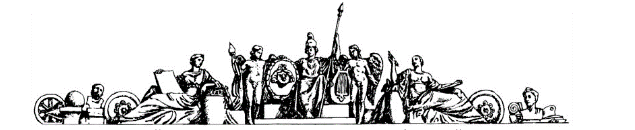
\includegraphics{6bauman}\\[1cm] % Include a department/university logo - this will require the graphicx package

%----------------------------------------------------------------------------------------

%----------------------------------------------------------------------------------------
%	HEADING SECTIONS
%----------------------------------------------------------------------------------------

\textsc{\LARGE МГТУ им. Баумана}\\[1.5cm] % Name of your university/college
\textsc{\Large Кафедра РЛ-5}\\[0.5cm] % Major heading such as course name
%\textsc{\large Minor Heading}\\[0.5cm] % Minor heading such as course title

%----------------------------------------------------------------------------------------
%	TITLE SECTION
%----------------------------------------------------------------------------------------

\HRule \\[0.4cm]
{ \huge \bfseries Лекции по дисциплине <<Конструирование оптико-электронных приборов>>}\\[0.4cm] % Title of your document
\HRule \\[1.5cm]
 
%----------------------------------------------------------------------------------------
%	AUTHOR SECTION
%----------------------------------------------------------------------------------------

\begin{minipage}{1\textwidth}
\begin{flushright} \large
%\emph{Подготовили:}\\
д.т.н., проф. каф. РЛ-5 \textsc{Городничев} В.А. \\ % Your name
ассистент каф. РЛ-5 \textsc{Филимонов} П.А.
\end{flushright}
\end{minipage}
%~
%\begin{minipage}{0.4\textwidth}
%\begin{flushright} \large
%\emph{Supervisor:} \\
%Dr. James \textsc{Smith} % Supervisor's Name
%\end{flushright}
%\end{minipage}\\[4cm]

% If you don't want a supervisor, uncomment the two lines below and remove the section above
%\Large \emph{Author:}\\
%John \textsc{Smith}\\[3cm] % Your name

\vfill % Fill the rest of the page with whitespace

%----------------------------------------------------------------------------------------
%	DATE SECTION
%----------------------------------------------------------------------------------------

{\large \the\year г.}\\[3cm] % Date, change the \today to a set date if you want to be precise




\end{titlepage}

\renewcommand{\contentsname}{\centerline{\Large{Cодержание}}}
%\tableofcontents
\chapter*{Введение}
\addcontentsline{toc}{chapter}{Введение}
Свойства электромагнитного излучения широко используются в современной науке и технике, особенно в бесконтактных, дистанционных устройствах контроля, измерения, передачи и преобразования информации, сбора и передачи энергии и др. Среди приборов, основанных на использовании электромагнитного излучения, особое место занимают ОЭП, которым свойственны высокая точность, быстродействие, возможность обработки многомерных сигналов и другие ценные для практики свойства.

Основная цель данной дисциплины, согласно учебной программе, состоит в содействии формированию и приобретению теоретических и практических навыков в области конструирования оптико-электронных приборов, а также развитию инженерного мышления. 

Задачами преподавания дисциплины, согласно учебной программе, являются: 
\begin{enumerate}
	\item изучение теоретических основ проектирования и конструирования ОЭП различного назначения;
	\item методов расчета и конструирования элементов и устройств ОЭП;
	\item способов выбора и обоснования критериев для оценки технических решений;
	\item освоения этапов проектирования ОЭП и разработки конструкторской документации на разных этапах в соответствии с требованиями стандартов ЕСКД;
	\item возможность развития научно-технического мышления будущего специалиста;
	\item формирования и развития творческого начала личности в процессе самостоятельной работы.
\end{enumerate} 

\chapter{Оптико-электронные приборы}
\section{Классификация ОЭП}
\textit{Оптико-электронными приборами} называются приборы, в которых информация об исследуемом или наблюдаемом объекте переносится оптическим излучением (содержится в оптическом сигнале), а ее первичная обработка сопровождается преобразованием этого излучения (оптического сигнала) в электрическую энергию (в электрический сигнал). В состав этих приборов входят как оптические, так и электронные звенья, причем и те и другие выполняют основные функции данного прибора, а не являются вспомогательными устройствами (например, узлами подсветки отсчетных шкал, устройствами термостабилизации).
Далее может встречаться также термин <<оптические приборы>>, что будет подразумевать --- <<оптические приборы, содержащие в своем составе механические, электронные и оптические функциональные устройства и элементы>>, т.е. фактически --- ОЭП.

ОЭП является сложной системой, включающей в себя большое число различных по своей физической природе и принципу действия звеньев -- аналоговых и цифровых преобразователей электрических сигналов, микропроцессоров, оптических, механических и электромагнитных узлов и др. Поэтому ОЭП часто называют оптико-электронными системами (ОЭС). 

Учитывая большое разнообразие ОЭП и их широкое применение в самых различных областях науки и техники  в курсе лекций рассмотрены общие для большинства ОЭП вопросы проектирования, достаточно общие и часто используемые на практике методы расчета и выбора основных параметров ОЭП, особенности конструкции и методы расчета параметров типовых узлов ОЭП.

Действие ОЭП основано на приеме и преобразовании электромагнитного излучения в различных диапазонах оптической области спектра. Одна из возможных обобщенных схем работы ОЭП представлена на рис.~\ref{pic:1OEPscheme}. Источник излучения естественного или искусственного происхождения создает материальный носитель полезной информации --- поток излучения.

Этим источником может быть сам исследуемый объект. Часто источник излучения дополняется передающей оптической системой, которая направляет поток на исследуемый объект или непосредственно в приемную оптическую систему (если наблюдается сам источник). Приемная оптическая система собирает поток, излучаемый наблюдаемым объектом или отраженный от него, формирует этот поток и направляет его на приемник излучения. Приемник превращает сигнал, переносимый потоком излучения (оптический сигнал), в электрический. Электронный тракт передает сигнал на выходной блок в виде, удобном для дальнейшей обработки или использования. Выходной блок формирует сигнал, по своим параметрам удовлетворяющий требованиям получателя информации.

Таким образом непосредственно в состав ОЭП входят: приемная оптическая система, приемник излучения, электронный и выходной блоки. 

В некоторых ОЭП после оптической системы может находиться анализатор изображения, которые в свою очередь могут быть: растровые и матричные, универсальные и сложные.

Помимо исследуемого объекта (<<полезный>> излучатель) на рис.~\ref{pic:1OEPscheme} показаны и возможные на практике <<вредные>> излучатели (фоны, помехи). Взаимное расположение звеньев может быть и несколько иным. Отдельные звенья на практике представляют собой весьма сложные устройства, например, в состав источника излучения могут входить передающая оптическая система, фильтры, модулятор. Иногда в состав ОЭП не входят некоторые из перечисленных звеньев. Это определяется, как правило, методом работы прибора.

Все ОЭП предназначены для получения информации об объектах окружающей среды, переносимой оптическими сигналами. Хорошо известны ОЭП, используемые для локации, исследования природных ресурсов, измерения оптических свойств различных объектов. Многие ОЭП работают в составе следящих систем, используемых в навигации и ориентации, в системах технического зрения, устройствах автоматического контроля и управления, системах управления летательными аппаратами, системах наведения и во многих других устройствах для измерения линейных, угловых величин и определения координат объектов. Определенной спецификой обладают оптико-электронные системы противодействия и подавления оптических схем противника.

Главный элемент --- оптическая система (ее сложно разработать, обеспечить нужное качество). С оптической схемы начинается разработка ОЭП.

\textit{Оптической схемой} называется графическое представление процесса изменения света в оптической системе.

Различия в принципах работы звеньев ОЭП, в способах обработки сигналов, проходящих через них, а также разнообразие условий эксплуатации ОЭП обусловливают сложность и многоступенчатость процесса проектирования этих приборов и требуют тщательного анализа как условий работы ОЭП, так и состояния имеющейся в распоряжении разработчика элементной базы.

Классификация ОЭП возможна по широкому кругу признаков в зависимости от принципов построения приборов и характера их применения (рис.~\ref{pic:1Classification}). К числу таких признаков могут быть отнесены параметры оптического сигнала, метод измерений, спектральный диапазон работы, режим работы, степень автоматизации, вид измерений, назначение и область применения, условия эксплуатации.


Как известно, в ОЭП носителем полезной информации служит оптический сигнал в виде потока излучения, являющийся функцией координат $(x, y, z)$ измеряемого объекта, спектрального состава излучения ($\lambda$), времени ($t$), состояния и положения плоскости поляризации излучения ($A_\text{п}$), т.е. $\Phi(x, y, z, \lambda, t, A_\text{п})$. 

В соответствии с параметрами оптического сигнала, принятыми в качестве основных при построении ОЭП, их можно разделить на:
\begin{itemize}
	\item радиометрические (фотометрические);
	\item спектральные;
	\item поляризационные;
	\item рефрактометрические;
	\item интерференционные;
	\item геометро-оптические.		
\end{itemize}

По методу работы ОЭП с учетом особенностей их построения и возможности управления параметрами излучения ОЭП делят на:
\begin{itemize}
	\item активные (наблюдаемый объект освещается (с помощью передающей оптической системы) лазером, при этом часть отраженного излучения поступает на вход ОЭП);
	\item полуактивные (один источник освещает все объекты);
	\item пассивные (используется собственное излучение исследуемого объекта; тепловое  (отраженное) от других источников излучения (солнца, луны); рассеянное излучение атмосферы и подстилающей поверхности).
\end{itemize}

В зависимости от спектрального состава используемого излучения ОЭП подразделяют на приборы, работающие в следующих областях спектра:
\begin{enumerate}
	\item ультрафиолетовая (УФ)~--- 200--380~нм ;
	\item видимая --- 400--700~нм;
	\item инфракрасная (ИК) --- 700 нм--1~мм.
\end{enumerate}

В свою очередь, УФ делится на: УФ-А (400--315 нм), УФ-Б (315--280 нм), УФ-С: (280--10 нм). Излучение с длиной волны менее 200 нм называют вакуумным ультрафиолетом, так как излучение не распространяется из-за полного поглощения в атмосфере.

ИК диапазон условно разделяют на: ИК-А или ближний ИК (700--1400 нм), ИК-Б или средний ИК (1400--3000 нм), ИК-С или дальний ИК (3 мкм--1 мм).

Важным признаком классификации является режим работы. В соответствии с этим ОЭП можно разделить на:
\begin{enumerate}
	\item индикационные;
	\item компенсационные;
	\item следящие.
\end{enumerate}

По степени автоматизации различают ОЭП:
\begin{enumerate}
	\item автоматические, работающие без участия оператора (обычно в следящем режиме);
	\item полуавтоматические, функционирование которых частично зависит от действий оператора;
	\item неавтоматические, выходная информация которых рассчитана на восприятие оператором.
\end{enumerate}

Существенные различия в принципах построения, функционирования и обслуживания имеют ОЭП, работающие в различных условиях эксплуатации. В соответствии с этим ОЭП подразделяют на:
\begin{enumerate}
	\item лабораторные;
	\item цеховые;
	\item полевые;
	\item бортовые.
\end{enumerate}

По виду измерений можно выделить:
\begin{enumerate}
	\item оптико-физические ОЭП, обеспечивающие измерение различных характеристик оптического излучения;
	\item угломерные;
	\item дальномерные;
	\item локационные ОЭП.
\end{enumerate}

Наиболее емким из приведенных признаков классификации является назначение (область применения). Практически невозможно найти область техники, где бы в настоящее время не применялись ОЭП. Поэтому в схеме классификации указаны только некоторые области техники, в которых применение ОЭП является решающим фактором их дальнейшего развития: 
\begin{enumerate}
	\item навигация (гирометры);
	\item геодезия (теодолит);
	\item астрофизика (телескопы);
	\item робототехника (система машинного зрения);
	\item телевизионная техника (подсветка и формирование изображения);
	\item медицина (микроскопы);
	\item контрольно-измерительная техника (интерферометры);
	\item военная техника (оптические прицелы).
\end{enumerate}

ОЭП внутри каждой из рассмотренных классификационных групп могут подразделяться по конструктивным, функциональным и иным признакам. Кроме того, между всеми классификационными признаками существуют прямые и косвенные связи. Например, контрольно-измерительные приборы могут быть угломерными, автоматическими, цеховыми.

\section{Основные критерии оценки качества ОЭП}

Качеством прибора (продукции) называется совокупность свойств прибора, обуславливающих его пригодность удовлетворять определенные потребности в соответствии с его назначением. Для объективной оценки качества прибора его свойства характеризуют количественно~--- показателями качества.

Критерии качества~--- это комплекс показателей, используемых для оценки свойств прибора, а также решений, принимаемых на различных этапах проектирования. Вследствие специфики ОЭП и разнообразия условий их производства оценка качества связана с рассмотрением широкого круга показателей, представленных на рис.~\ref{pic:1QualityOEP}.


Всесторонняя оценка современных изделий может быть выполнена лишь при комплексном учете всех указанных показателей. Вместе с тем при проектировании разработчики чаще всего оценивают качество будущего прибора по показателям функционирования, надежности и технологичности.

\textit{Показатели функционирования} являются основными, они характеризуют техническую сущность прибора, и именно поэтому они стоят на первом месте в техническом задании.

Ввиду большого разнообразия ОЭП показатели функционирования могут быть самыми различными. Достаточно обобщенными являются информационные характеристики, к которым относят:
\begin{enumerate}
	\item входной язык, посредством которого осуществляется связь прибора с наблюдаемым или контролируемым объектом;
	\item энергия, необходимая для формирования единицы информации;
	\item функция преобразования, описывающая зависимость информативного параметра выходного сигнала от информативного параметра входного сигнала при номинальных значениях неинформативных параметров;
	\item выходной язык, посредством которого осуществляется связь прибора с потребителем информации;
	\item скорость выдачи информации прибором и восприятия ее потребителем (быстродействие).
\end{enumerate}

Наряду с перечисленными к показателям функционирования могут быть отнесены также вид потребляемой энергии и мощность потребления, габаритные размеры и масса прибора.

\begin{flushleft}
\textbf{Требования к надежности}
\end{flushleft}

Сложность ОЭП, включающих оптические, механические и электронные узлы, требования к работоспособности этих приборов в резко изменяющихся условиях эксплуатации ставят перед конструктором задачу~--- создать прибор, обладающий высокой надежностью в течение всего срока службы.

\textit{Надежность} определяется как свойство объекта сохранять во времени в установленных пределах значения всех параметров, характеризующих способность выполнить требуемые функции в заданных режимах и условиях применения, технического обслуживания, ремонта, хранения и транспортирования. 

Надежность прибора зависит от количества и качества входящих в него элементов, условий работы (температуры, влажности, механических воздействий), схемного и конструктивного выполнения прибора, технологии изготовления и качества материала элементов.

\begin{flushleft}
\textbf{Показатели технологичности}
\end{flushleft}

\textit{Технологичность деталей, узлов и конструкций, удобство сборки} может быть охарактеризована следующими показателями: 
\begin{itemize}
\item минимальными затратами труда на изготовление;
\item минимальным ассортиментом средств изготовления;
\item минимумом сложных и трудоемких производственных процессов;
\item простотой подготовки производства;
\item минимальным числом операций и временем их проведения;
\item правильным выбором допусков на изготовление;
\item простотой монтажа деталей в узлы без дополнительной обработки;
\item законченностью узлов, входящих в прибор;
\item простотой сборки прибора в целом.
\end{itemize}

\textit{Рациональный выбор материалов}: материалы, необходимые для изготовления деталей, следует выбирать с учетом не только функциональных и эксплуатационных особенностей прибора, но и технологии его изготовления. Для единичного производства целесообразно использовать материалы, хорошо поддающиеся обработке резанием. При крупносерийном и массовом производстве более экономичны способы изготовления без снятия стружки, что и определяет в значительной степени выбор материалов.

\textit{Минимальная номенклатура элементов, материалов, полуфабрикатов} упрощает снабжение производства. 
Кроме того, необходимо иметь в виду, что некоторые детали и элементы часто не соответствуют специфике и профилю предприятия. В этих случаях целесообразнее идти по пути кооперации с другими предприятиями, чем осваивать производство соответствующих изделий.

\textit{Обеспечение взаимозаменяемости деталей, узлов и блоков} предполагает идентичность конструктивных и присоединительных размеров, соединителей, а также входных и выходных параметров. Взаимозаменяемость позволяет обеспечить замену одного узла или блока другим без дополнительной подгонки и регулирования. Это обстоятельство имеет важное значение при сборке приборов, особенно при крупносерийном и массовом производстве, а также при обслуживании и ремонте приборов. Прежде всего необходимо стремиться к взаимозаменяемости электронных узлов и блоков. Взаимозаменяемость обеспечивается рациональными допусками на размеры и параметры узлов и блоков.

\textit{Максимальная нормализация и унификация конструкций} основана на применении нормализованных, унифицированных или стандартизованных деталей и узлов. Нормализованные детали включены в нормаль данного предприятия или группы родственных предприятий. Унифицированные детали применяются на предприятиях всей отрасли промышленности. Стандартизованные детали используются на предприятиях различных отраслей промышленности.

Унифицированные и стандартизованные детали, узлы и блоки изготовляются централизованно, что позволяет автоматизировать процесс их производства, обеспечить высокую надежность и минимальную стоимость. Показатели унификации и стандартизации характеризуют степень использования и применения в данном приборе стандартизованных, унифицированных и заимствованных узлов и деталей. Чем больше таких элементов будет в проектируемом приборе, тем меньше затраты на их конструирование, технологическую подготовку производства, выше, как правило, надежность функционирования, проще организовать обслуживание и ремонт.

\textit{Обеспечение возможности изготовления деталей при единичном и мелкосерийном производстве на универсальном оборудовании} имеет смысл при изготовлении уникальных и экспериментальных приборов, для выпуска которых в единичных образцах или малыми сериями нецелесообразно делать специальную технологическую оснастку. Повысить качество таких приборов и уменьшить технологические и трудовые затраты на их изготовление можно путем использования типовых узлов и деталей, о которых говорилось выше.

\textit{Простота и удобство выполнения сборки, монтажа и юстировки} имеет особое значение для качественной настройки прибора, как в заводских условиях, так и в процессе дальнейшего использования. При этом снижаются трудовые затраты и требования к уровню подготовки производственного и обслуживающего персонала, а также требования к сложности юстировочного и стендового оборудования.

\textit{Эстетические показатели} характеризуют внешний вид прибора, его соответствие современному стилю, гармоничность сочетания отдельных элементов прибора друг с другом, соответствие формы прибора его назначению, качество и совершенство отделки внешних элементов, поверхностей и упаковки, выразительность и качество надписей, знаков, технической документации (проспекта, каталога, инструкции, паспорта).

\textit{Патентно-правовые показатели} характеризуют степень новизны заложенных в ОЭП технических решений а также вопросы патентно-правовой  защиты и определяются патентоспособностью и патентной чистотой. Патентоспособным является решение, которое может быть признано изобретением в одной или нескольких странах. Патентной чистотой обладают решения, не попадающие под действие (не нарушающие прав) других патентов.

\textit{Показатели техники безопасности} характеризуют степень защищенности людей и животных от опасного воздействия ОЭП (защита от электрического удара, электромагнитных полей, теплового воздействия, радиации, оптических излучений, шума, токсичных и газовых выделений, вибраций), а также самих приборов от климатических, механических, биологических и других воздействий на них. Такими показателями, например, являются категория и класс исполнения и эксплуатации.

\textit{Экономические показатели} выражаются прежде всего в стоимости прибора. К основным факторам, определяющим стоимость прибора, относятся область применения, условия эксплуатации, технологичность конструкции, требования по надежности, серийность выпуска, стоимость материалов и комплектующих изделий, простота и удобство обслуживания, юстировок и ремонта. Экономические показатели характеризуют уровень затрат на производство и эксплуатацию ОЭП. Среди них выделяют полную себестоимость и оптовую цену прибора. 

\textit{Эргономические показатели} характеризуют степень приспособленности прибора к взаимодействию с человеком с позиции удобства работы, гигиены, безопасности труда. 

Эргономические показатели разделены на гигиенические (уровень шума, амплитуда и частота вибраций, уровень радиации, температура, степень загазованности, токсичности), антропометрические (размеры и расположение экранов, индикаторов, рукояток, наглазников, налобников, форма сиденьев), психофизиологические (диапазоны усилий на рукоятках, скорость выполнения движений, уровень освещенности, цвет и яркость световых сигналов, тембр и сила звуковых сигналов), психологические (объем и интенсивность потока информации, количество и частота выполняемых операций, количество и расположение контрольных, сигнальных, управляемых элементов).

Экологические показатели характеризуют степень вредного влияния на окружающую среду и ее загрязнение при изготовлении, эксплуатации и утилизации приборов.

\section{Основные требования, предъявляемые к ОЭП}
\textbf{Требования по внешним условиям и условиям эксплуатации}: к внешним условиям, оказывающим влияние на работу ОЭП, могут быть отнесены климатические факторы, механические воздействия, возникающие при транспортировании и эксплуатации, различные виды силовых полей, действие ионизирующего излучения.

В процессе эксплуатации различают два режима:
\begin{itemize}
	\item сохранение работоспособности ОЭП при воздействии дестабилизирующих факторов с экстремальными значениями (устойчивость);
	\item обеспечение работоспособности ОЭП в нормальных условиях после воздействия на неработающий прибор дестабилизирующих факторов с экстремальными значениями (прочность, стойкость).
\end{itemize}

Наиболее разнообразно влияние климатических факторов: температуры, влажности, давления окружающей среды, воздействия твердых и газообразных примесей, солнечного излучения, ветровой нагрузки, биофакторов.

\textit{Температура окружающей среды} оказывает существенное влияние на работу приборов, так как при ее изменении практически все элементы и детали ОЭП меняют свои свойства. Диапазон температур, в котором приходится работать ОЭП, весьма широк. Даже в земных условиях возможны перепады температуры воздуха от $-80^{\circ}$C (в Антарктиде) до $+55^{\circ}$C (в тропических районах). При прямом воздействии Солнца температура нагретой поверхности может быть значительно выше. В отдельных случаях требуется обеспечить нормальную работу прибора в еще более жестких температурных условиях. Например, температура на поверхности Венеры достигает $300^{\circ}$С, а в условиях космического пространства при затенении от солнечного излучения близка к абсолютному нулю.

Большинство ОЭП эксплуатируется в нормальных температурных условиях. Для многих видов приборов, используемых на открытом воздухе, требуется обеспечить нормальную работу в интервале температур $-50\ldots+50^{\circ}$С. В отдельных случаях требуется обеспечение работы приборов в экстремальных условиях, указанных выше.

При недостаточном учете влияния перепадов температуры возможны ухудшение качества оптического изображения из-за термооптических аберраций и смещения плоскости изображения за счет температурных деформаций, появление расклеек в компонентах, разрушение оптических деталей вследствие разности показателей расширения оптических материалов и материалов оправ.

Тепловые воздействия на электронные элементы проявляются, в частности, в изменении параметров приемников излучения, номинальных значений параметров и характеристик электрорадиоэлементов, нарушении контактов и пробоях в изоляционных материалах.

В кинематических цепях при изменении температуры возможны ухудшение прочности материалов, повышение трения за счет изменения зазоров и вытекания или загустения смазочного материала. При неравномерном нагреве или охлаждении могут появляться деформации, приводящие к заклиниванию кинематических механизмов.

Весьма серьезные последствия оказывает на приборы попадание \textit{влаги}. Наличие влаги может привести к запотеванию оптических деталей, особенно в сочетании с резким изменением температуры. Пары воды, вступая в химическую реакцию с материалами, приводят к коррозии металлов, изменению физико-химических свойств специальных покрытий оптических деталей и изоляционных материалов. Под воздействием влаги ухудшаются контактные соединения за счет окисления контактов.

При проектировании предусматривают меры по защите приборов от воздействия влаги. Часто с этой целью приборы герметизируют, а внутренний объем осушают продувкой сухого очищенного воздуха. Могут применяться также специальные влагопоглотители.

\textit{Давление} окружающей среды оказывает заметное влияние на функционирование ОЭП. При понижении давления воздуха падает значение напряжения пробоя, что особенно важно помнить при использовании высоковольтных элементов. Кроме этого, существенно возрастает скорость испарения смазочного материала, что может привести к повышению трения и заклиниванию элементов кинематики прибора. В связи с уменьшением давления отвод теплоты за счет конвекционного переноса падает, в результате чего резко возрастает вероятность перегрева элементов прибора. Поэтому необходимо либо применять специальные материалы и элементы, рассчитанные на работу в условиях пониженного давления, либо осуществлять герметизацию прибора с созданием нормального рабочего давления внутри.

На работу ОЭП оказывают влияние не только рассмотренные выше климатические факторы, но и содержащиеся в воздухе \textit{песок и пыль}. Их механическое воздействие в сочетании с воздействием влаги и нагрева иногда приводит к значительному ухудшению характеристик приборов. 

В сочетании с ветровым воздействием наличие в воздухе частиц песка и пыли приводит к абразивному разрушению полированных и окрашенных поверхностей. При этом вследствие матирующего эффекта возможен выход из строя оптических систем.

Для приборов, эксплуатируемых на открытом воздухе, необходимо учитывать \textit{воздействие солнечного излучения}, приводящее к перегревам, нарушениям лакокрасочных покрытий, усилению коррозии при одновременном воздействии кислорода и влаги воздуха, быстрому старению резины, пластмасс и электрической изоляции.

При длительной эксплуатации и хранении приборов, а также при эксплуатации в тропических условиях следует учитывать \textit{влияние биофакторов}, к которым относятся плесневые грибы, насекомые и грызуны. Развитие плесени ухудшает механические и электрические параметры приборов, а также пропускание оптических деталей. Борьба с влиянием этого фактора сводится к герметизации и осушке внутренних объемов приборов, применению стекол группы А, защите оптических деталей специальными покрытиями, использованию фунгицидов. Кроме того, могут быть использованы такие методы, как придание корпусам и наружным деталям простой формы без углублений, пазов, выступов, которые способствуют скоплению грязи и пыли и затрудняют чистку приборов.

Важное значение при конструировании ОЭП имеет учет \textit{влияния механических воздействий}, к которым относятся вибрация, ударные воздействия, транспортировочные перегрузки. При этом следует иметь в виду, что наряду с внешними источниками воздействий на элементы прибора могут оказывать влияние вибрация и удары, обусловленные внутренними источниками, например несбалансированностью вращающихся частей, неточностью изготовления, зазорами, разрушениями соприкасающихся кинематических элементов.

В результате воздействий указанных факторов возможны разрушения отдельных элементов, деталей и паек, нарушение контактов реле, переключателей, потенциометров и коллекторов, повреждение изоляции с возникновением замыканий, самоотвинчивание резьбовых соединений, появление трещин, сколов в оптических и других хрупких деталях.

Механическая прочность конструкции обеспечивается применением соответствующих материалов, способов соединения деталей и может быть повышена за счет использования различных элементов жесткости: косынок, приливов, ребер.

Для предотвращения самоотвинчивания крепежных изделий либо применяют различные фиксаторы, либо устанавливают крепежные детали с использованием клеев, компаундов и герметиков. 

В случаях, когда указанные меры оказываются недостаточными, для защиты от механических воздействий используются демпферы и амортизаторы.

При работе ОЭП подвергаются \textit{воздействию различных полей}: электрического, магнитного, электромагнитного СВЧ, в результате чего могут возникать паразитные наводки, приводящие к ухудшению работы прибора. Источники полей могут находиться как вне, так и внутри прибора. Подавление наводок в большинстве случаев сводится к устранению или ослаблению паразитных связей между источником и приемником наводок путем экранирования и развязывания цепей.

Для защиты от электрических полей или подавления паразитной емкостной связи во всех диапазонах частот используют тонкие листы и пленки, а также проволочные сетки и решетки из материала с хорошей электрической проводимостью.

Для экранирования магнитных низкочастотных полей используют материалы с высокой магнитной проницаемостью (пермаллой, альсифер, технически чистое железо).

Для экранирования высокочастотных полей используют экраны из хорошо проводящих материалов (медь, латунь, алюминий). При действии полей СВЧ на основной материал экрана наносят слой серебра для повышения его электрической проводимости. Для защиты от наводок все электрические связи между блоками, по которым передаются измерительные сигналы, необходимо осуществлять экранированными проводами. Принципы расчета и конструирования защитных экранов изложены в соответствующей литературе.

Иногда ОЭП используются в условиях \textit{воздействия ионизирующего излучения} (на атомных электростанциях для дистанционного наблюдения, при космических исследованиях). Такие приборы должны отвечать требованиям радиационной стойкости. При воздействии ионизирующего излучения имеют место радиационные и поляризационные эффекты, приводящие к ухудшению оптических свойств материалов, нарушению работы полупроводниковых и электровакуумных приборов, изменению проводимости воздушных промежутков и диэлектрических материалов. При конструировании ОЭП, работающих в указанных условиях, прежде всего необходимо применять радиационно-стойкие материалы и элементы.

К ОЭП могут предъявляться также специфические требования, связанные с условиями эксплуатации. К их числу можно отнести, например, такие, которые вытекают из особенностей приборов, эксплуатируемых в состоянии невесомости, глубоко под водой, в шахтах и т.п. Кроме того, в некоторых ОЭП отдельные блоки могут работать в нормальных условиях, а остальные~-- в крайне неблагоприятных. Все эти особенности должны оговариваться при разработке ТЗ.

Таким образом, в современных условиях конструктору приходится иметь дело с широким кругом требований, которые находятся в тесном взаимодействии и часто противоречат друг другу, что приводит к многовариантности проектных решений.
%\chapter{Проектирование ОЭП} 

\textit{Проектирование}~--- разработка проектной, конструкторской и другой технической документации, предназначенной для создания новых видов и образцов продукции промышленности.

\textit{Цель проектирования}~--- разработка нового изделия.

В процессе проектирования происходит поиск вариантов создания оптико-электронных приборов, его возможных конструкций, разработка и уточнение схем, теоретическое и экспериментальное исследование характеристик предполагаемых инженерных решений.

\textit{Конструирование} является составной частью проектирования и заключается в разработке конкретного варианта изделия на основе проведенных предварительных исследований. При этом создается конструкция проектируемого изделия: устройство, состав, взаимное расположение частей и элементов, способ их соединения и взаимодействия с учетом используемых материалов, технологии изготовления.

В процессе проектирования выпускают чертежи сборочных единиц и деталей, схемы, рассчитывают допуски на погрешности и технологию изготовления и сборки деталей, устанавливают технические условия на прибор, составляют техническое описание, разрабатывают другую конструкторскую документацию, необходимую для изготовления и эксплуатации изделия.

\section{Уровни проектирования}
Разработка сложных систем, какими являются ОЭП, проводится в определенной последовательности.

Отправной точкой создания любой системы являются выбор и формулировка цели проектирования. Необходимость создания нового изделия определяется как развитием конкретного направления техники, так и запросами потребителей (научных и производственных учреждений, человека-оператора). 

Обоснование исходных данных требует учета назначения системы, основных видов ее взаимодействия с другими системами или подсистемами, если она является подсистемой, входящей в состав другой более крупной системы, влияния внешних факторов.

В результате указанного рассмотрения должна быть получена полная совокупность исходных данных для проектирования прибора. 

Результатом проделанной работы является техническое задание~(ТЗ) на прибор, после утверждения которого можно переходить к собственно проектированию.

\newpage
Различают следующие основные уровни проектирования:
\begin{itemize}
	\item информационно-логический;
	\item системотехнический;
	\item схемотехнический;
	\item конструкторский;
	\item технологический.
\end{itemize}

Первые три уровня иногда объединяют в единый функциональный, или схемный уровень проектирования.
\begin{flushleft}
	\textbf{Информационно-логический уровень}
\end{flushleft}

В процессе проектирования на информационно-логическом уровне определяется конкретная структура данного прибора, определяются связи функциональных устройств между собой и устанавливаются требования технических заданий на проектирование отдельных функциональных устройств, исходя из требований ТЗ на прибор в целом. ТЗ на проектирование того или иного устройства содержит требования к сигналам, информации и командам, вырабатываемым этим устройством.

Таким образом, проектирование на этом уровне состоит из определения сначала структуры проектируемого объекта, а затем в определении оптимальных значений параметров этой структуры, т.е. составляющих ее элементов.

\begin{flushleft}
	\textbf{Системотехнический уровень}
\end{flushleft}

На системотехническом уровне функционального проектирования производится проектирование отдельных функциональных устройств, т.е. процесс разбивается на отдельные ветви. Каждое из функциональных устройств рассматривается здесь как структура, состоящая из взаимосвязанных функциональных блоков. Процесс проектирования заключается в определении оптимального состава и параметров блоков, например, оптической системы, приемника излучения, электронного тракта, системы отображения.

Все эти отдельные блоки рассматриваются на этом уровни как преобразователи сигналов, безотносительно к их внутреннему устройству. Здесь определяются требования к преобразованию сигналов тем или иным блоком, т.е. к его передаточным и прочим характеристикам.
\begin{flushleft}
	\textbf{Схемотехнический уровень}
\end{flushleft}

На схемотехническом уровне производится проектирование отдельных блоков, входящих в состав функциональных устройств, в соответствии с техническими заданиями, определенными на предыдущем уровне.

Каждому блоку соответствует своя ветвь, причем, начиная с этого уровня, различные ветви имеют различную «специализацию» в соответствии с физической природой блоков, игнорируемой на предыдущем уровне.

Схемотехнический уровень является важнейшим при функциональном проектировании.\\ В настоящее время он занимает наибольший объем работы и именно на этом уровне определяются основные параметры различных схем прибора, в конечном итоге обеспечивающие правильную работу прибора в соответствии с техническим заданием. Например, на этом уровне выделяется оптическая ветвь и производится расчет оптической системы прибора.

Целью проектирования оптической системы на этом уровне является определение как ее структуры, т.е. количества входящих в нее элементов и их типов, так и численных значений параметров этих элементов.

На электронной ветви схемотехнического уровня производится проектирование электронных схем блоков, преобразующих сигналы. Здесь, как и на оптической ветви, определяется структура схемы, т.е. состав и соединения ее функциональных элементов (резисторов, конденсаторов, транзисторов, интегральных схем), а затем и значения их параметров.

На механической ветви производятся аналогичные действия по проектированию кинематической схемы какого-либо устройства прибора.

Таким образом, в процессе схемотехнического проектирования разработчик определяет элементную базу будущего прибора.

Как показывает практика, очень часто проектирование новых элементов на этом уровне не требуется, и работа сводится к подбору элементов из имеющихся стандартных или покупных.

Рассмотренные уровни функционального проектирования являются типичными для ОЭП средней сложности. В более простых случаях некоторые уровни могут исключаться, например, информационно-логический или системотехнический.

\begin{flushleft}
	\textbf{Конструкторский уровень}
\end{flushleft}

Конструкторское проектирование, или просто конструирование, идет обычно параллельно функциональному проектированию или с некоторым отставанием и является важнейшей ветвью процесса проектирования, поскольку именно здесь оптико-электронный прибор приобретает не только схемную, но и материальную (правда пока только в документации) реализацию. Разработчик, работающий на этом уровне, называется обычно просто конструктором. 

В большинстве проектных организаций эти два уровня проектирования выполняются разными людьми и даже разными подразделениями. Так, например, проектирование оптической системы (оптической схемы) прибора выполняет обычно оптик-расчетчик или оптик-вычислитель, работающий в специализированном оптическом вычислительном бюро. Результатом этого проектирования является оптический выпуск, содержащий всю необходимую информацию об оптической схеме, включая ее параметры и их допустимые отклонения. 

На основании этой информации другой разработчик --- конструктор оптик-механик --- выполняет конструирование соответствующего оптического узла, например, объектива, диафрагм, механизма фокусировки объектива. Он выпускает чертежи всех деталей этого объектива, включая оптические сборочные чертежи отдельных узлов и объектива в целом.

Естественно, что этот процесс может быть итерационным. Так, в случае, если конструктору никак не удается надежно закрепить какую-либо оптическую деталь из-за неудачных с конструктивной точки зрения ее параметров, например, слишком крутых радиусов кривизны, приходится возвращаться на ветвь функционального проектирования и пересчитывать оптическую схему с изменением ее параметров.

Аналогичная картина наблюдается для электронных и кинематических схем. После того, как они разработаны на уровне функционального проектирования, конструктор материализует эти схемы в виде определенного монтажа на печатной плате, в виде деталей и узлов механизма.

Конструирование, также как и функциональное проектирование, разделяется на уровни.

Верхний уровень -- это компоновочный, на котором определяется общая компоновка всего прибора, взаимное расположение его отдельных узлов.

Один или несколько следующих уровней, в зависимости от сложности прибора --- это уровни узлов (сборочных единиц), где разрабатываются конструкции отдельных частей прибора. Сразу за компоновочным уровнем процесс конструирования может разделяться на ветви, соответствующие различным узлам, например: механическим, оптико-механическим, электронным или электромеханическим узлам. И, наконец, последний уровень --- это уровень деталей, на котором разрабатываются и выпускаются рабочие чертежи отдельных деталей.

\newpage
\begin{flushleft}
	\textbf{Технологический уровень}
\end{flushleft}

На уровне технологического проектирования производится разработка технологических процессов изготовления прибора. Как и на других стадиях разработки, здесь выделяются различные уровни:
\begin{itemize}
	\item верхний уровень -- испытание прибора (методики испытаний);
	\item уровень юстировки прибора (достижение верного взаиморасположения элементов);
	\item уровень сборки всего прибора;
	\item техпроцессы сборки, юстировки, контроля сборочных единиц;
	\item техпроцессы изготовления деталей. 
\end{itemize}

Верхним уровнем является уровень испытаний прибора, на котором разрабатываются методики испытаний прибора на соответствие различным пунктам ТЗ.

Следующим идет уровень юстировки, где разрабатываются методики юстировки прибора.

Затем уровень сборки всего прибора, который разветвляется по отдельным узлам (сборочным единицам). На этих уровнях разрабатываются техпроцессы сборки, юстировки и контроля различных сборочных единиц прибора. Наконец, на низших уровнях разрабатываются технологические процессы изготовления отдельных деталей.

Результатами работы на ветви технологического проектирования являются технологические карты, методики юстировки и контроля.

\section{Проектирование с использованием системного подхода}
Сущность системного подхода состоит в том, что объект проектирования рассматривается как система, т.е. как единство взаимосвязанных элементов, которые образуют единое целое и действуют в интересах реализации единой цели. 

Системный подход включает в себя выявление структуры системы, типизацию связей, определение свойств (атрибутов) системы, анализ влияния внешней среды, он требует рассматривать каждый элемент системы во взаимосвязи и взаимозависимости с другими элементами, вскрывать закономерности, присущие данной конкретной системе, выявлять оптимальный режим ее функционирования. 

Системный подход проявляется прежде всего в попытке создать целостную картину исследуемого или управляемого объекта. Исследование или описание отдельных элементов при этом производится с учетом роли и места элемента во всей системе.

Процесс функционирования сложной системы происходит на многих уровнях. Система расчленяется на подсистемы, которые представляют собой компоненты, необходимые для существования и действия системы.

Методическим средством реализации системного подхода к проектированию служит системный анализ, под которым понимается совокупность приемов и методов исследования объектов (процессов) посредством представления их в виде систем и их последующего анализа.

Системный анализ предполагает системный подход и к изучению связей между элементами, между подсистемами и системой.
\newpage
В основе системного подхода лежат следующие основные принципы и положения:
\begin{enumerate}
	\item Принцип цели: при разработке конструкции исходят из необходимости учета требований и показателей, которые должны быть реализованы. Должна быть ясна цель проектирования.
	\item Принцип целостности: объект рассматривается как единая система, состоящая из устройств, сборочных единиц элементов, функциональных устройств.
	\item Иерархичность строения: всякая система допускает разделение на подсистемы, что приводит к ступенчатости конструкции. Выявление и представление иерархии структуры объекта проводится с целью установления связей между частями объекта.
	\item Необходимо обобщение опыта и оценка перспектив развития систем данного или близких классов.
	\item Всестороннее рассмотрение взаимодействия системы с внешней средой и учет основных видов взаимодействия элементов и узлов внутри системы.
	\item Выбор критерия и показателей качества. Установление перспектив развития объектов.
	\item Правильное сочетание различных методов проектирования, в первую очередь, математических, эвристических и экспериментальных. Итерационный метод проектирования.
\end{enumerate}

\section{Блочно-иерархический подход к проектированию}
Если в системном подходе прибор рассматривается как сложная система, состоящая из связанных и взаимодействующих частей, то при блочно иерархическом подходе прибор рассматривается как иерархическая структура, состоящая из большого количества уровней и ветвей, наподобие некоторого опрокинутого дерева (рис.~\ref{pic:2block}).
\begin{figure}[H]
	\caption{Блочно-иерархическая структура}
	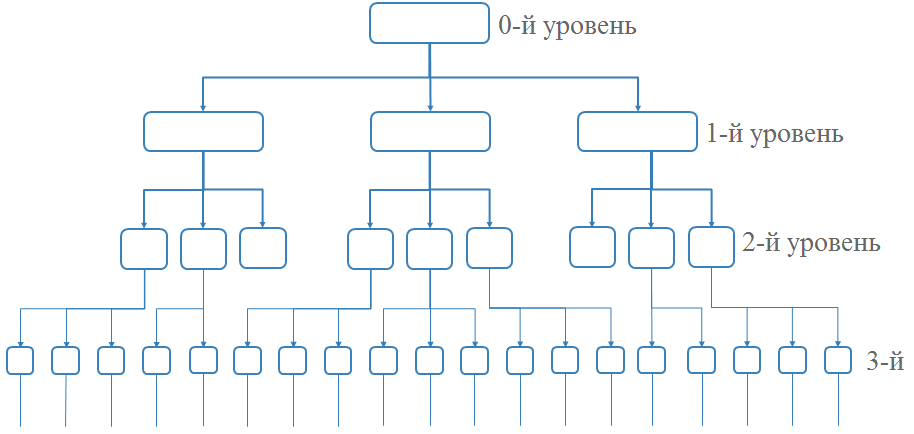
\includegraphics[width=1\textwidth]{2block.png}
	\label{pic:2block}
\end{figure}

В соответствии с блочно-иерархическим подходом в объекте проектирования может быть выделен ряд иерархических уровней (рис.~\ref{pic:2block}). На верхнем уровне подлежащий проектированию сложный объект состоит из ряда менее сложных элементов (например, для ОЭП -- приемная система, электронный блок обработки сигналов с выхода приемника излучения). Указанные элементы на более низком иерархическом уровне, в свою очередь, являются системами элементов менее сложной структуры (например, в приемную оптическую систему могут входить объектив, компенсатор, анализатор изображения, сканирующий блок). 

Далее подобное разделение на элементы может продолжаться до некоторого уровня, на котором дальнейшее разделение становится уже невозможным. Элементы, полученные на этом уровне, по отношению к объекту проектирования являются базовыми. Применительно к ОЭП такими базовыми элементами будут детали (оптические, механические) и различные комплектующие изделия (электро- и радиоэлементы, подшипники, электродвигатели).

Иерархия составных частей ОЭП при блочно-иерархическом подходе:
\begin{enumerate}
	\item Приборное устройство (или его конструируемая часть).
	\item Функциональная единица.
	\item Сборочная единица --- изделие, составные части которого подлежат соединению между собой сборочными операциями.
	\item Детали --- изделие, изготовленное из однородного (по наименованию и марке) материала без применения сборочных операций. (Или неделимые однородные тела, состоящие из элементов формы (геометрических поверхностей тел) и материала).
\end{enumerate}

Общий процесс проектирования при таком подходе представляется в виде движения по рассматриваемому дереву, при котором выполняются элементарные проектные операции на каждом уровне и на каждой ветви, т.е. структура проектирования также является блочно-иерархической, причем на каждом уровне и ветви процесс проектирования имеет дело с небольшим количеством элементов, рассматриваемых как целые, благодаря чему этот процесс достаточно несложен и вполне реализуем при нормальных ресурсах. Весь процесс проектирования, сплетающийся в виде блочно-иерархической структуры таких элементарных процессов, также теперь становится вполне реализуемым.

Такая структура позволяет осуществлять общий процесс проектирования, используя различные направления движения по блочно-иерархическому дереву. В зависимости от направления движения различают нисходящее, восходящее и смешанное проектирование.

Нисходящее проектирование, как следует из его названия, начинается с верхнего уровня, где прибор рассматривается как целое, затем проектируется его структура первого уровня, затем второго. Результатом проектирования на данном уровне является техническое задание для проектирования на следующем, более низком уровне.

Нисходящее проектирование всегда гарантирует выполнение требований технического задания на каждом уровне и поэтому должно бы считаться наиболее рациональным, но на каком-то уровне процесс проектирования может остановиться из-за того, что при существующих физических, технических, технологических или экономических ограничениях решение обратной задачи и соблюдение технического задания данного уровня становится невозможным. 

В этом случае приходится возвращаться на предыдущий уровень или даже выше, искать там другое решение своей обратной задачи, а затем опять пробовать вернуться на тот уровень, на котором процесс остановился, но с уже другим техническим заданием. Таким образом, блочно-иерархическая структура, позволяя в принципе реализовать процесс проектирования, делает неизбежным его итерационный характер, заключающийся в возврате к повторению проектирования на предыдущих уровнях с измененными условиями.

Восходящее проектирование выполняется в обратном порядке; при этом происходит как бы сборка отдельных узлов, а затем сборка всего прибора. Восходящее проектирование, как нетрудно увидеть, обычно гарантирует реализуемость проекта на любом уровне, но отнюдь не гарантирует соблюдения всех требований технического задания, поэтому процесс может остановится на каком-либо уровне из-за несоблюдения требований технического задания высшего уровня. При этом необходим возврат на предыдущие низшие уровни с попыткой <<собрать>> структуру данного уровня из других элементов. Таким образом и восходящее проектирование также неизбежно имеет итерационный характер.

При смешанном проектировании по части ветвей мы имеем нисходящий процесс, а по части~-- восходящий, которые в определенных точках встречаются. Итерационный характер такого проектирования также очевиден.

Из рассмотренных процессов предпочтительным является все-таки нисходящее проектирование. На практике, особенно для сложных приборов, процесс проектирования носит обычно смешанный характер с преобладанием нисходящих потоков, а восходящее проектирование применяется к тем частям приборов, которые собираются из стандартных, хорошо отработанных деталей, элементов и узлов.

Из рассмотренного становится ясен также эвристический характер проектирования, т.е. невозможность его полной алгоритмизации, автоматизации, поскольку ввиду сложности процесса и невозможности заранее определить полностью его ход необходимо принимать решения на основании опыта, интуиции, с привлечением творческих способностей разработчика, т.е. на базе так называемого алгоритма принятия решения. 

Все этапы проектирования выполняются на основе ТЗ. В случае, когда проектирование объекта проводится по сформулированным на более высоком иерархическом уровне ТЗ, оно носит название внутреннего. Внешнее проектирование предполагает разработку ТЗ на систему высшего иерархического уровня. При внешнем проектировании необходим правильный учет современного состояния техники, возможностей технологии, перспектив их развития, экономических факторов.
%\chapter[Регламентация конструкторских работ при проектировании ОЭП.\\ Конструкторская документация]{Регламентация конструкторских работ при проектировании ОЭП. Конструкторская документация}

Организация процесса проектирования определяется степенью новизны и сложностью решаемой задачи. В зависимости от степени новизны различают:
\begin{itemize}
	\item частичную модернизацию существующего прибора (системы), приводящую к некоторому улучшению одного или нескольких показателей качества за счет изменения параметров, улучшения элементной базы, частичного изменения структуры;
	\item существенную модернизацию, приводящую к значительному улучшению основных показателей качества прибора (системы) за счет существенного изменения параметров и структурной схемы, приводящих к большим конструктивным изменениям;
	\item создание нового прибора (системы), предназначенного для решения известных или принципиально новых задач и основанного на новых принципах действия, использование которых позволяет резко улучшить основные показатели качества.
\end{itemize}

При создании новых ОЭП процессу собственно проектирования~-- опытно-конструкторским работам (ОКР)~-- обычно предшествуют научно-исследовательские работы (НИР).

Целью НИР является решение проблемных вопросов, позволяющее обосновать возможность и целесообразность дальнейшего проектирования, получить необходимую исходную информацию и тем самым предотвратить значительные затраты на проведение проектных работ в случае, когда поставленная задача не может быть решена предлагаемыми средствами.

В рамках НИР изучается состояние разработок по поставленной или родственным задачам. С этой целью анализируются все доступные источники информации, а также опыт промышленности. На основе выдвинутых теоретических положений разрабатываются макеты узлов и прибора в целом. После их изготовления и экспериментальных исследований дается заключение о возможности создания промышленного образца прибора и формулируются рекомендации по проведению ОКР.

Последовательность разработки и изготовления промышленных изделий в настоящее время регламентируется группой государственных стандартов, входящих в Единую систему конструкторской документации (ЕСКД).

ЕСКД устанавливает единый порядок разработки, выполнения, оформления, согласования, внесения изменений, учета и хранения конструкторской документации.

В соответствии с действующим стандартом (ГОСТ~2.103–68) проектирование ОЭП можно представить в виде последовательности этапов, в процессе которых разрабатывают ТЗ, техническое предложение, эскизный, технический и рабочий проекты.

Перечисленные этапы позволяют обеспечить изготовление опытного образца, который затем испытывается. По результатам испытаний в конструкцию вносятся необходимые изменения и уточнения, и после окончательных испытаний дается заключение о возможности изготовления установочной серии приборов. В зависимости от потребностей в данном приборе в дальнейшем осуществляется переход к мелкосерийному, серийному или массовому производству.

Следует отметить, что в зависимости от назначения и области применения прибора (системы), необходимых сроков разработки, а также в связи с внедрением современных методов системного и автоматизированного проектирования последовательность и содержание этапов могут изменяться. Например, если на этапе технического предложения получено полное представление о схемном и конструктивном решении прибора, этап эскизного проектирования может не выполняться, и разработчик сразу переходит к техническому проектированию. Для ускорения процесса проектирования иногда могут быть совмещены технический и рабочий проекты. Однако при создании большинства современных приборов указанная последовательность проектирования выдерживается.

\section{Техническое задание}
Проектирование любого промышленного изделия, в том числе и ОЭП, ведется на основании технического задания (ТЗ).

\textit{ТЗ} -- это документ, который устанавливает назначение и область применения, технические, качественные и технико-экономические требования, а также определяет необходимые стадии разработки конструкторской документации и ее состав.

ТЗ составляется организацией-заказчиком при возможном участии организации-разработчика с привлечением других заинтересованных организаций. После утверждения и согласования ТЗ принимается к выполнению.

ТЗ на проектирование ОЭП обычно состоит из нескольких разделов.

Вводная часть ТЗ содержит основание для проведения ОКР. В следующем разделе указываются назначение и область применения изделия. Далее излагаются технические требования, предъявляемые к изделию.

К техническим требованиям относятся:
\begin{itemize}
	\item диапазон и точность измерений; 
	\item дальность действия;
	\item чувствительность или разрешающая способность; выходные параметры прибора, обеспечивающие его стыковку с другими системами (если данный ОЭП входит в состав какого-либо комплекса), либо форма представления информации об измеряемой величине (напряжение, код, вход в ЭВМ), если прибор решает самостоятельную задачу. При этом могут предъявляться требования к крутизне и диапазону линейности выходных характеристик прибора;
	\item спектральный диапазон работы, параметры и характеристики излучения исследуемого или измеряемого объекта;
	\item конструктивные требования к схемам и узлам прибора (кинематическим, электрическим, оптическим);
	\item габаритные размеры и масса прибора или отдельных его частей;
	\item требования по видам потребляемой энергии и мощности потребления;
	\item требования к тепловыделению прибора, а при необходимости охлаждения -- параметры системы охлаждения;
	\item требования по соответствию параметров прибора или его конструктивного исполнения определенным ГОСТам, ОСТам и другим нормативным документам.
\end{itemize}

 
В соответствующем разделе дается полная характеристика условий работы изделия, среди которых можно назвать:
\begin{itemize}
	\item характер помех, определяемый либо конкретным указанием их энергетических, спектральных и пространственных характеристик, либо указаниями общего порядка (например, облачное небо, звездный фон, вид ландшафта);
	\item параметры или характеристики, определяющие прохождение излучения для ОЭП, работающих в полевых или других неблагоприятных условиях (например, данные о среде распространения и ее параметрах, метеорологической дальности видимости, наличии задымленности);
	\item характер размещения прибора и в связи с этим различные динамические факторы условий эксплуатации (вибрация, перегрузки, ударные воздействия);
	\item динамические свойства исследуемого объекта -- частота колебаний, перемещения, распределение параметров по гармоническим составляющим и др.;
	\item метеорологические факторы -- температурный диапазон, влажность, давление, воздействие осадков, пыли, морского тумана, солнечной радиации;
	\item требования к защите прибора от воздействия полей и излучений;
	\item условия хранения и транспортирования;
	\item диапазон возможных отклонений параметров системы энергопитания.
\end{itemize}
 
В специальном разделе ТЗ излагаются требования по надежности и работоспособности, в том числе:
\begin{itemize}
	\item гарантийный срок службы прибора при обусловленных ТЗ условиях эксплуатации;
	\item периодичность проверок, аттестаций и профилактического ремонта;
	\item режимы работы, в частности время непрерывной работы, периодичность включения;
	\item время готовности прибора к работе от момента включения электропитания;
	\item требования к надежности работы в течение определенного времени с требуемой вероятностью безотказной работы;
	\item требования к жесткости, надежности крепления элементов и узлов, системе амортизации;
	\item требования к безопасности работы с прибором.
\end{itemize}

В ТЗ включаются также разделы, в которых излагаются требования по охране труда, технической эстетике, технологичности, отражаются технико-экономические показатели, специальные требования, учитывающие специфику построения, применения и изготовления прибора.

В одном из заключительных разделов ТЗ отражаются этапы создания прибора и состав технической документации, разрабатываемой на каждом этапе и ОКР в целом, другие аспекты проектирования, имеющие принципиальное значение. После оформления и утверждения ТЗ приступают непосредственно к проектным работам.

Следует отметить, что в процессе выполнения ОКР техническое задание может уточняться по взаимному согласованию заинтересованных сторон в случаях, если будет доказана необоснованность каких-либо требований, показана принципиальная невозможность обеспечения некоторых свойств.

\section{Техническое предложение}

В соответствии с действующим стандартом (ГОСТ~2.118–73) Техническое предложение разрабатывают в целях выявления дополнительных или уточненных технических и эксплуатационных требований к прибору, которые не были отражены в ТЗ и для обоснования которых целесообразно выполнить предварительную конструкторскую проработку и анализ различных вариантов решения.

Наиболее типичными видами работ, проводимых на этапе технического предложения, являются:
\begin{itemize}
	\item научно-технический поиск в целях подбора и изучения всех доступных  материалов по проектируемому изделию;
	\item анализ полученной информации и выявление положений, позволяющих наметить варианты решения поставленной в ТЗ задачи;
	\item установление возможных вариантов схемы и конструкции прибора;
	\item сравнительная, оценка выявленных вариантов по различным показателям, определенным ТЗ;
	\item проверка вариантов на патентную чистоту и конкурентоспособность, оформление заявок на изобретение;
	\item проверка соответствия возможных вариантов требованиям стандартизации, унификации, техники безопасности, эргономики;
	\item предварительная оценка технологичности конструкции прибора.
\end{itemize}

В процессе выполнения указанных работ на данном этапе могут быть проведены различные расчеты, а также экспериментальные исследования с использованием математических моделей и макетов. Для изготовления макетов должна быть разработана конструкторская документация.

Результатом работ на данном этапе должно быть ТЗ, сформулированное с учетом положений, выявленных в процессе теоретических и экспериментальных исследований, а также конструкторская документация (КД), дающая обобщенное представление о выявленных технических решениях.

На рассматриваемом этапе наряду с учетом конструктивных и эксплуатационных особенностей существующих изделий аналогичного назначения необходимо иметь в виду тенденции и перспективы развития отечественной и зарубежной техники в данной области.

Следует уже при проведении данного этапа проектирования стремиться к выбору оптимального варианта прибора, так как это позволит избежать ненужных затрат на последующих этапах и ускорит проектирование. В случае невозможности такого выбора необходимо установить дополнительные требования к последующим этапам.

Конструкторская документация, выпускаемая на этапе технического предложения, включает обобщенные схемы ОЭП, упрощенные чертежи общего вида, габаритный чертеж, ведомость технического предложения, пояснительную записку, патентный формуляр.

Пояснительная записка в соответствии с действующим стандартом (ГОСТ~2.106-68) в общем случае должна включать следующие разделы:
\begin{itemize}
	\item введение (с указанием документов, на основании которых выполняется проектирование);
	\item назначение и область применения  прибора;
	\item технические характеристики прибора;
	\item описание и обоснование выбранной конструкции;
	\item расчеты, подтверждающие работоспособность и надежность выбранного конструктивного решения;
	\item описание организации работ с применением разрабатываемого прибора;
	\item ожидаемые технико-экономические показатели;
	\item уровень оценки по показателям стандартизации, унификации, патентной чистоты.
\end{itemize}

Указанная структура пояснительной записки применима к любому этапу проектирования. При этом в зависимости от особенностей изделия и характера решаемых на том или ином этапе проектирования задач возможно объединение, исключение или введение новых разделов.

Пояснительная записка должна быть оформлена в соответствии с действующим стандартом~(ГОСТ~2.105-79). Чертежи и схемы выполняются с максимальными упрощениями, предусмотренными ЕСКД.

После рассмотрения и утверждения технического предложения его материалы служат основой для проведения последующих этапов проектирования.

\section{Эскизное проектирование}
Эскизный проект ОЭП разрабатывается в целях получения его принципиальных схемных и конструктивных решений. Конструкторская документация, полученная в результате эскизного проектирования, должна давать общее представление об устройстве и принципе работы прибора и особенностях его использования.

Требования к эскизному проекту регламентируются по ГОСТ~2.119-73.

При выполнении эскизного проекта проводят:
\begin{itemize}
	\item проработку возможных вариантов схемного и конструктивного решений прибора;
	\item расчетное обоснование их ожидаемых технических характеристик;
	\item оценку возможности реализации полученных вариантов на основе освоенной промышленностью номенклатуры материалов и комплектующих изделий;
	\item оценку технологичности конструкции и возможностей изготовления прибора в условиях конкретной производственной базы;
	\item проверку принятых технических решений на патентную чистоту и оформление заявок на изобретения в случае положительных результатов патентных исследований;
	\item проверку решений на соответствие требованиям техники безопасности, стандартизации и унификации;
	\item проработку художественно-конструкторских вопросов, оценку прибора по показателям эргономики.
\end{itemize}

С учетом полученных результатов перечисленных работ выполняется сравнительная оценка вариантов по установленным ТЗ показателям и обобщенным критериям оценки качества ОЭП и выбирается оптимальный вариант прибора.

На этапе эскизного проектирования на основе принятых принципиальных решений большое внимание уделяется выявлению на основе принятых принципиальных решений новых изделий и материалов, которые планируется разработать и изготовить другими предприятиями (например, источников и приемников излучения, электромеханических элементов, шарико-подшипников, конструкционных и других материалов). На этом этапе должны быть составлены технические требования к таким изделиям и материалам и определен круг их возможных разработчиков.

С целью более обоснованного выбора оптимального варианта прибора может быть проведено макетирование его отдельных узлов или прибора в целом с последующим исследованием макетов.

Важное значение при эскизном проектировании имеет оценка метрологического обеспечения будущего серийного или массового производства прибора. Это прежде всего относится к прецизионным приборам, поскольку для оценки их точностных возможностей может потребоваться уникальное оборудование (стенды). В некоторых случаях для создания такого оборудования необходимы значительные усилия, вплоть до проведения самостоятельных НИР и ОКР, на выполнение которых должно быть выдано соответствующее ТЗ.

Иногда уже на этапе эскизного проектирования предварительно решают вопросы упаковки и транспортирования, например при проектировании крупногабаритных изделий или изделий, для которых требуется специальная упаковка или средства транспортирования.

На этапе эскизного проектирования при необходимости выполняют и другие работы. В то же время обычно не повторяют работы, проведенные на этапе технического предложения, если они не могут дать дополнительных данных. В этом случае результаты ранее проведенных работ отражаются в пояснительной записке.

\textit{Конструкторская документация эскизного проекта} ОЭП включает основные схемы прибора, чертеж его общего вида и основных сборочных единиц, габаритный чертеж, ведомость эскизного проекта, пояснительную записку.

\textit{Схемы прибора} разрабатывают на основе выбранного принципа его работы и проведенных расчетов. Как правило, выполняются функциональные или принципиальные схемы следующих видов: оптические, электрические, кинематические. Схемы должны давать полное представление о принципе работы прибора, взаимосвязях всех его узлов и элементов.

\textit{Чертеж общего вида} выполняется с упрощениями, предусмотренными ЕСКД, и должен давать представление о компоновке прибора, взаимодействии его основных составных частей. При эскизном проектировании на чертеже общего вида часто используют контурное изображение заимствованных сборочных единиц, покупных и других комплектующих изделий (объективов, электродвигателей, подшипников).

\textit{Габаритный чертеж} представляет собой контурное (упрощенное) изображение прибора с габаритными, установочными и присоединительными размерами и является необходимым конструкторским документом, если прибор входит в состав каких- либо сложных систем, комплексов или должен быть установлен (смонтирован) на специальных основаниях. Габаритный чертеж разрабатывается по согласованию со смежными организациями и окончательно уточняется на этапе технического проекта.

\textit{Пояснительная записка} эскизного проекта выполняется с учетом следующих требований к содержанию разделов.

При изложении технической характеристики наряду с указанием свойств прибора приводятся сведения об отклонениях или соответствии требованиям ТЗ и сравнительные данные отечественных и зарубежных аналогов.

Раздел <<Описание и обоснование выбранной конструкции>> наряду с изложением принятых схемных и конструктивных решений может содержать сведения о макетах прибора, методике и результатах их испытаний, сведения о технологичности, дополнительные результаты патентных исследований, сведения о вновь разрабатываемых материалах и комплектующих изделиях.

Пояснительная записка эскизного проекта должна содержать все необходимые расчеты ОЭП, подтверждающие возможность его реализации. При большом объеме расчетов они могут быть оформлены в виде отдельного документа. При этом в пояснительной записке приводятся только результаты расчетов.
К числу наиболее важных относятся следующие виды расчетов ОЭП: энергетический (светотехнический); оптической системы (габаритный, аберрационный); электронного тракта; точности. В зависимости от принципа работы ОЭП проводят и другие расчеты, часто имеющие принципиальное значение: кинематический, динамический, надежности, прочности и жесткости, температурных режимов.

Приложение к пояснительной записке может включать сведения по стандартизации и унификации, материалы художественно-конструкторской проработки, в частности результаты эргономического анализа, требования по технике безопасности и другие материалы, представляющие интерес для всесторонней характеристики проектируемого прибора.

Эскизный проект рассматривается заинтересованными организациями и защищается в установленном порядке. Выявленные в результате рассмотрения и защиты замечания либо устраняются, либо по ним намечаются мероприятия для последующих этапов проектирования, после чего протокол о защите утверждается.

\section{Техническое проектирование}

Цель технического проектирования состоит в выявлении окончательных технических решений, дающих полное представление о конструкции прибора. Требования к техническому проекту определяются действующим стандартом (ГОСТ~2.120-73).

Основными видами работ являются:
\begin{itemize}
	\item детальная разработка конструкции всего прибора и его составных частей;
	\item разработка принципиальных схем, на основе которых могут быть выполнены монтажные схемы, схемы соединений, осуществлены сборка и настройка оптических и электронных блоков;
	\item окончательное оформление заявок и ТЗ на изготовление новых изделий и материалов;
	\item выявление номенклатуры покупных изделий и согласование их применения;
	\item окончательное согласование габаритных, установочных и присоединительных размеров, мест подключения разъемов с заказчиком и основными потребителями;
	\item анализ конструкции прибора, его узлов и отдельных наиболее сложных и ответственных деталей на технологичность и определение на основе этого анализа возможности использования имеющегося на предприятии оборудования, необходимости приобретения или создания нового технологического оборудования и спецоснастки;
	\item окончательное решение вопросов метрологического обеспечения по выбору средств измерений и методов контроля метрологических характеристик приборов;
	\item проверка принятых технических решений на соответствие требованиям стандартизации, унификации, техники безопасности;
	\item проверка приборов на патентную чистоту, оформление заявок на изобретения;
	\item окончательное решение вопросов транспортирования, хранения и монтажа на месте эксплуатации;
	\item оценка эксплуатационных характеристик приборов, в частности взаимозаменяемости, удобства обслуживания, ремонтопригодности, устойчивости к воздействию факторов внешней среды, возможности быстрого устранения отказов, контроля качества работы, обеспеченности средствами контроля технического состояния и др.
\end{itemize}

Как правило, разработка технического проекта сопровождается большим объемом макетирования. Макеты создаются в целях проверки конструктивных и схемных решений прибора, а также для подтверждения окончательно принятых решений. 

При этом наряду с функционирующими макетами целесообразно делать макеты-муляжи (например, из дерева), на которых можно проверить удобство обслуживания и расположения элементов, т. е. отработать эргономические и художественно-конструкторские показатели.

Выполняемые при техническом проектировании расчеты служат для окончательного установления свойств прибора, выработки требований к узлам и отдельным ответственным деталям. На этом этапе проектирования уточняются такие показатели, как инструментальная составляющая суммарной погрешности, которая может быть выявлена только на основе окончательно принятых конструктивных решений. 

Особое внимание уделяется подбору необходимого оборудования для лабораторных испытаний будущих приборов.

В результате технического проектирования обычно выпускается следующая \textit{конструкторская документация}: чертежи общего вида прибора и его сборочных единиц, габаритный чертеж, чертежи всех схем, ведомость технического проекта, пояснительная записка, приложение к пояснительной записке, ведомость покупных изделий, ведомость согласования применения покупных изделий, патентный формуляр, карта технического уровня.

Пояснительная записка технического проекта включает те же разделы, что и записка к эскизному проекту. Однако в ней особое внимание уделяется обоснованию и описанию конструктивных особенностей прибора, принципов его функционирования, В нее включаются расчеты, выполненные по ходу технического проекта, Существенно расширяется раздел, посвященный описанию организации работ с прибором на месте эксплуатации. В этом разделе даются сведения о приемах и способах работы с прибором, транспортировании, монтаже и хранении, количестве и квалификации обслуживающего персонала.

В приложении к пояснительной записке могут быть приведены расчеты, материалы ху\-до\-жест\-вен\-но-конструкторской проработки.

Технический проект подлежит защите и утверждению заказчиком.

\section{Рабочее проектирование}
Рабочий проект выполняется с целью создания и отработки полного комплекта конструкторской документации ОЭП, достаточной для изготовления опытного образца прибора. Рабочее проектирование может выполняться как самостоятельный этап, но иногда для ускорения процесса проектирования его начинают на этапе технического проекта (технорабочий проект). Этап рабочего проектирования характеризуется тесным взаимодействием конструкторских и технологических подразделений предприятия.

Основными видами работ на этом этапе являются:
\begin{itemize}
	\item детальная разработка конструкции прибора и его узлов с указанием технологических требований к сборке и юстировке;
	\item доведение всех схем до рабочего состояния (выполняются монтажные схемы, на оптических схемах приводятся требования по юстировке);
	\item составление спецификаций и сводных ведомостей покупных и стандартных изделий и деталей, марок и сортаментов применяемых материалов;
	\item разработка ведомостей и чертежей согласования применения готовых изделий;
	\item согласование методик юстировки, настройки, монтажа, испытаний;
	\item составление технического описания, технических условий, инструкций по эксплуатации, формуляра, технического паспорта;
	\item составление ведомости запасного инструмента и принадлежностей (ЗИП);
	\item разработка технологических процессов изготовления наиболее сложных и ответственных деталей.
\end{itemize}

\textit{Рабочие чертежи} должны обеспечивать возможность оптимального применения стандартных, покупных и освоенных ранее изделий, рационально ограниченную номенклатуру материалов, покрытий, размеров, резьб, допусков, необходимую степень взаимозаменяемости, экономичные способы изготовления, максимальное удобство при эксплуатации.

В процессе рабочего проектирования выполняются контрольно-сборочные чертежи узлов и прибора в целом для выявления ошибок в рабочих чертежах деталей до их изготовления и сборки. Контрольно-сборочный чертеж вычерчивают по рабочим чертежам деталей путем считывания всех необходимых размеров, проверки правильности простановки допусков на сопрягаемые детали и тщательного переноса размеров в соответствии с необходимым масштабом на поле чертежа.

Все выявленные ошибки и неточности рабочих чертежей устраняются, после чего чертежи проходят нормоконтроль по действующему стандарту (ГОСТ~2.111-68), технологический контроль и утверждаются.

Рабочие чертежи деталей и сборочные чертежи являются основной документацией, руководствуясь которой можно осуществить изготовление \textit{опытного образца} прибора. Дополнением к ним являются технические условия, содержащие все отсутствующие в чертежах, но необходимые для изготовления и отладки технические требования, а также требования на приемку и испытания.

Технические условия составляют в соответствии с ГОСТ~2.114-70 на основе ТЗ, чертежей и документации технического проекта.
Составление методики юстировки и настройки должно быть увязано с выпуском рабочих чертежей контрольно-юстировочной аппаратуры.

После подготовки и утверждения всей необходимой документации опытное производство предприятия изготавливает опытный образец или партию приборов. Конструкторские подразделения предприятия осуществляют наблюдение за ходом изготовления и оказывают необходимую помощь производству. Возникающие в процессе изготовления замечания к документации исправляются.

Изготовленные опытным производством образцы приборов передаются на всесторонние испытания. При проведении предварительных испытаний проверяют правильность функционирования, соответствие приборов техническим условиям и техническому паспорту. Эти испытания могут проводиться как в условиях заводской испытательной лаборатории (на соответствующих стендах), так и в условиях предполагаемой эксплуатации. Если изготовленные приборы прошли предварительные испытания, их передают на государственные испытания для полной проверки опытного образца прибора на соответствие ТЗ и техническим условиям. Так же, как и предварительные, государственные испытания могут проводиться в лабораторных и полевых условиях.

Государственные испытания осуществляются под руководством государственной комиссии, состоящей из специалистов отраслевых НИИ, представителей заказчика и предприятия-раз\-ра\-бот\-чи\-ка. Испытания регламентируются специальной программой. Государственным испытаниям подвергаются приборы, прошедшие предварительные испытания и снабженные всей необходимой технической документацией, что подтверждается соответствующим актом.

В процессе государственных испытаний фиксируются все замечания. Если они легко устранимы, то испытания продолжаются; если носят принципиальный характер, то опытные образцы и документация возвращаются на доработку, после которой вновь представляются на испытания.

По окончании испытаний составляется акт, где дается заключение о соответствии прибора ТЗ и о возможности его запуска в серийное или массовое производство, а также приводятся замеченные недостатки, которые должны быть устранены в процессе подготовки прибора к следующему этапу производства.

Перед серийным производством обеспечивается технологическая подготовка производства, заключающаяся в проектировании технологического процесса изготовления деталей и сборки, конструировании и изготовлении технологической оснастки, разработке методики контроля технических характеристик прибора и проектировании соответствующей контрольно-юс\-ти\-ро\-воч\-ной аппаратуры.

По окончании этапа технологической подготовки производства может быть изготовлена установочная партия приборов, на которой окончательно отрабатываются конструкторская документация и технологический процесс, а также проверяются наличие требуемых технологической оснастки и контрольно-юстировочной аппаратуры и их возможности. При соответствии установочной партии приборов и технической документации предъявляемым требованиям приборы запускаются в серийное производство.

\section{Конструкторская документация}
На всех этапах жизненного цикла (разработка -- производство -- эксплуатация) ОЭП сопровождает техническая документация (ТД). Состав этой документации и ее содержание регламентируется Государственными стандартами. В настоящее время в стране действует большое количество стандартов, которые сгруппированы по направлениям жизненного цикла изделий в следующие комплексы:
\begin{itemize}
	\item единая система конструкторской документации (ЕСКД);
	\item единая система технологической документации (ЕСТД);
	\item единая система программной документации (ЕСПД);
	\item единая система технологической подготовки производства (ЕСТПП);
	\item единая система защиты изделий и материалов от коррозии, старения и биоповреждений (ЕСЗКС).
\end{itemize}

Государственные стандарты, входящие в ЕСКД, устанавливают взаимосвязанные единые правила и положения по порядку разработки, оформления и обращения конструкторской документации на изделия, разрабатываемые и выпускаемые предприятиями всех отраслей промышленности.

\textit{Конструкторские документы (КД)} -- графические и текстовые документы, в отдельности или в совокупности определяющие состав и устройство изделия и содержащие необходимые данные для его разработки и изготовления, контроля, приемки, эксплуатации, ремонта, утилизации.

Стандартам ЕСКД присваивают обозначения по классификационному принципу. Номер стандарта составляется из цифры, присвоенной классу стандартов ЕСКД, одной цифры после точки, обозначающей классификационную группу стандартов в соответствии с таблицей 1, числа, определяющего порядковый номер стандарта в данной группе, и двузначной цифры (после тире), указывающей год регистрации стандарта. Например, обозначение стандарта ЕСКД <<ЕСКД. Схемы. Виды и типы. Общие требования к выполнению>> имеет вид:
\begin{description}
	\item[ГОСТ 2.701-84]:
	\item[ГОСТ] -- категория нормативно-технического документа (государственный стандарт);
	\item[2] -- класс (стандарты ЕСКД);
	\item[7] -- классификационная группа стандартов; 
	\item[01] -- порядковый номер стандарта в группе; 
	\item[84] -- год регистрации стандарта.
\end{description}
 
Разработка и изготовление любого ОЭП связаны с выпуском конструкторской документации, которая полностью и однозначно определяют все необходимые и достаточные данные для изготовления, настройки и юстировки, приемки, эксплуатации и ремонта как всего прибора в целом, так и его составных частей.
 
\begin{table}[h]
	\caption{Перечень классификационных групп стандартов ЕСКД}
	\label{tab:vrema_zhizni_neodnorodnostey}
	\begin{tabular}{|c|l|} \hline 
		\parbox[t]{1.5cm}{\centering Шифр\\ группы} & \parbox[t]{14cm}{\centering Содержание стандартов в группе} \\ \hline
		0 & Общие положения \\ \hline
		1 & Основные положения \\ \hline
		2 & Классификация и обозначение изделий в КД \\ \hline
		3 & Общие правила выполнения чертежей \\ \hline
		4 & \parbox[t]{14cm}{Правила выполнения чертежей изделий машиностроения\\ и приборостроения} \\ \hline
		5 & \parbox[t]{14cm}{Правила обращения КД (учет, хранение, дублирование,\\ внесение изменений)} \\ \hline
		6 & Правила выполнения эксплуатационной и ремонтной документации \\ \hline
		7 & Правила выполнения схем \\ \hline
		8 & \parbox[t]{14cm}{Правила выполнения документов строительных,\\ судостроительных и горных дел} \\ \hline
		9 & Прочие стандарты \\ \hline
	\end{tabular}
\end{table}

Согласно действующему стандарту (ГОСТ~2.102-68) к конструкторской документации относятся следующие графические и текстовые документы:
\begin{itemize}
	\item чертеж детали, содержащий изображение детали и другие данные, необходимые для ее изготовления и контроля;
	\item сборочный чертеж (СБ), содержащий изображение сборочной единицы и другие данные, необходимые для ее сборки и контроля;
	\item чертеж общего вида (ВО), определяющий конструкцию прибора, взаимодействие его основных составных частей, поясняющий принцип работы изделия, включая форму деталей и характерные размеры, которые облегчают уяснение формы элементов деталей, содержащий предельные отклонения сопрягаемых поверхностей и сопровождаемый техническими требованиями к прибору;
	\item теоретический чертеж (ТЧ), определяющий геометрическую форму прибора и координаты расположения составных частей;
	\item габаритный чертеж (ГЧ), представляющий собой контурное (упрощенное) изображение прибора с габаритными, установочными и присоединительными размерами;
	\item монтажный чертеж (МЧ) -- упрощенное изображение прибора с данными, необходимыми для его установки на месте эксплуатации;
	\item схемы по действующему стандарту (ГОСТ 2.701-84), на которых показаны в виде условных изображений или обозначений составные части изделия и связи между ними;
	\item спецификация -- документ, определяющий состав сборочной единицы, комплекса или комплекта. Спецификация в общем случае состоит из разделов: документация, комплексы, сборочные единицы, детали, стандартные изделия, прочие изделия, материалы, комплекты. Требования к выполнению спецификаций регламентирует действующий стандарт (ГОСТ 2.108-68);
	\item ведомости спецификаций (ВС), ссылочных документов(ВД), покупных изделий (ВП), согласования применения изделий (ВИ), держателей подлинников (ДП), технического предложения (ПТ), эскизного проекта (ЭП), технического проекта (ТП);
	\item пояснительная записка (ПЗ) содержит описание прибора и принципа его действия, а также обоснование принятых при разработке прибора технических и технико-экономических решений;
	\item технические условия (ТУ) содержат требования к прибору и его составным частям и деталям и обычно включают следующие разделы: вводную часть с указанием назначения, области применения прибора и условий его эксплуатации; состав комплекта прибора; технические требования к материалам, отдельным деталям, сборочным единицам и прибору в целом; требования к покрытиям и окраске; методы контроля технических характеристик, порядок приемки, поверок и испытаний; требования к транспортированию и хранению, смазыванию, упаковке; порядок маркировки; указания о гарантийных обязательствах изготовителя;
	\item программа и методика испытаний (ПМ);
	\item патентный формуляр (ПФ);
	\item карта технического уровня и качества изделия (КУ), характеризующая уровень качества прибора, соответствие его технических и экономических показателей достижениям науки и техники и потребностям народного хозяйства;
	\item таблицы (ТБ);
	\item расчеты (РР);
	\item инструкции (И), представляющие собой документы, используемые при изготовлении прибора (сборке, регулировании, контроле, приемке).
\end{itemize}

Помимо конструкторских документов в соответствии с ГОСТ 2.601-68 разрабатывается комплект эксплуатационных документов, в том числе:
\begin{itemize}
	\item техническое описание (ТО), дающее общее представление о приборе, его технических характеристиках, принципе его работы и устройстве, комплектации и другие сведения;
	\item инструкция по эксплуатации (ИЭ), которая может быть частью технического описания, но может быть и самостоятельным документом. В инструкции приводятся методика работы с прибором и его поверки, правила монтажа, подготовки прибора к работе, обращения с прибором, разборки, чистки, смазывания, транспортирования, а также указания по технике безопасности;
	\item технический паспорт (ПС) и формуляр (ФО) -- документы, сопровождающие прибор в процессе эксплуатации. Технический паспорт включает основные номинальные технические характеристики прибора, результаты исследования технических характеристик, состав комплекта, свидетельство о приемке, положения о гарантиях и сведения о рекламациях, номер прибора и номера комплектующих изделий. В формуляре наряду с основными сведениями, приведенными в паспорте прибора, даются сведения о режиме работы, учете времени эксплуатации, отметки о текущем состоянии прибора, его техобслуживании и ремонте;
	\item ведомость ЗИП (ЗИ) устанавливает номенклатуру, назначение и количество запасных частей, инструментов, принадлежностей и материалов, необходимых при эксплуатации и ремонте прибора;
	\item ведомость эксплуатационных документов (ЭД).
\end{itemize}

Состав ремонтных документов определяется ГОСТ~2.602-68. Эти документы предусматривают технически возможное и экономически целесообразное восстановление технических параметров прибора при эксплуатации на различных стадиях.

Важное место в конструкторской документации ОЭП принадлежит схемам. В соответствии с ГОСТ~2.701-84 виды схем обозначаются буквами, а их типы -- цифрами. В оптико-электронном приборостроении используются в основном схемы следующих видов:
\begin{description}
	\item[Э] -- электрические;
	\item[К] -- кинематические;
	\item[Л] -- оптические;
	\item[С] -- комбинированные.
\end{description}

Схемы в зависимости от их типа имеют следующие обозначения:
\begin{description}
	\item[1] -- структурные;
	\item[2] -- функциональные;
	\item[3] -- принципиальные;
	\item[4] -- соединений;
	\item[5] -- подключения;
	\item[6] -- общие;
	\item[7] -- расположения.
\end{description}

Например, схема электрическая функциональная имеет шифр Э2.

Специфическими конструкторскими документами ОЭП являются комбинированная функциональная и оптическая принципиальная схемы.

Функциональная комбинированная схема иллюстрирует процессы преобразования сигналов, происходящие в функциональных цепях прибора и в приборе в целом. Эта схема является основным документом, раскрывающим принцип работы прибора. При выполнении функциональных схем ОЭП руководствуются следующими положениями.

Функциональная схема выполняется без соблюдения масштаба, действительное пространственное расположение составных частей прибора либо не учитывается вообще, либо учитывается приближенно.

При выполнении функциональной комбинированной схемы могут быть использованы условные обозначения, применяемые при выполнении схем других видов (оптических, кинематических, электрических). Схема должна быть выполнена компактно, но без ущерба для ясности и удобства чтения.

Элементы и узлы схемы, являющиеся отдельными функциональными частями, допускается изображать в виде прямоугольников с указанием вида элемента и его характеристик.

При выполнении схемы необходимо пользоваться условными графическими изображениями, установленными ГОСТами. При отсутствии соответствующего стандартизованного условного обозначения элемент на схеме изображают либо в виде, приближенно соответствующем его конструктивному исполнению, либо в виде прямоугольника, внутри которого написано название элемента.

Условные графические обозначения, стандартизованные или построенные на основе стандартизированных обозначений, на схемах не поясняются. Элементы, составляющие функциональные группы или устройства, на схемах допускается выделять штрих-пунктирными линиями, указывая внутри контура наименование или тип группы. Для наглядности допускается изображать элементы схем различных видов, а также отдельные элементы и устройства, не входящие в данный прибор, но необходимые для пояснения принципа его работы.

Технические характеристики элементов или частей схемы следует указывать рядом с графическим обозначением или на свободном поле схемы. На схеме могут быть поясняющие надписи, диаграммы, таблицы, определяющие последовательность процессов во времени.

Механические связи между элементами схемы указываются штриховой линией, электрические и оптические -- сплошной. 

Оптические схемы выполняются в соответствии с ГОСТ~2.412-81 в определенном масштабе.

При разработке ОЭП выполняются и другие схемы, перечисленные выше, если они необходимы.

Структурная схема определяет основные функциональные части изделия, их назначение и взаимосвязи. 

Принципиальная схема определяет полный состав элементов и связей между ними и, как правило, дает детальное представление о принципах работы изделия. 

Схема соединений показывает соединения составных частей изделия и определяет провода, жгуты и кабели, которыми осуществляются эти соединения, а также места их присоединения и ввода (зажимы, соединители, фланцы).
Схема подключения показывает внешнее подключение изделия. 

Общая схема определяет составные части комплекса и соединения их между собой на месте эксплуатации. 

Схема расположения задает относительное положение составных частей изделия, а при необходимости проводов, жгутов, кабелей, светопроводов.

Все перечисленные схемы могут быть использованы при разработке других конструкторских документов, а также при эксплуатации приборов. Правила выполнения схем регламентируются соответствующими стандартами ЕСКД, относящимися к 7-й группе.

При разработке рабочих чертежей деталей, сборочных, общих видов, габаритных и монтажных чертежей, при оформление текстовых документов необходимо руководствоваться действующими стандартами (ГОСТ~2.109-73, ГОСТ~2.108-68, ГОСТ~2.106-68).

Каждый конструкторский документ должен иметь определенное обозначение в соответствии с обезличенной классификационной системой обозначений изделий и документов. Обозначение изделия и его основного конструкторского документа (спецификации и чертежа детали) имеет следующую структуру: индекс организации-разработчика; классификационная характеристика; порядковый регистрационный номер. К обозначениям всех остальных документов добавляются шифры (например, СБ, Э2, ЛЗ, ТУ).

В соответствии с действующим стандартом (ГОСТ~2.501-88) все подлинники, дубликаты и копии конструкторской документации подлежат учету и хранению в отделе технической документации (ОТД). Подлинник для сдачи в ОТД должен иметь необходимые подписи, подтверждающие его соответствие нормам, и предусмотренные согласования со всеми заинтересованными службами. Вносить изменения в конструкторскую документацию или аннулировать ее имеет право только предприятие - держатель подлинников. Основой для этого служит <<Извещение об изменении>>. Изменяемые размеры, слова, знаки, надписи, как правило, зачеркивают так, чтобы можно было легко прочитать зачеркнутое, и рядом с зачеркнутым проставляют новые данные.

\begin{flushleft}
	\textbf{Кодирование и идентификация технической документации}
\end{flushleft}

Для обеспечения документооборота внутри предприятия, беспрепятственного обмена документацией между предприятиями без ее переоформления, автоматизации разработки технической документации с унификацией машинно-ориентированных форм документов, совершенствования способов учета, хранения и изменения документации вводится код документа -- уникальный для каждого документа цифро-буквенный код, однозначно соответствующий только этому документу. В документ могут вноситься изменения, однако его код должен оставаться неизменным. Факт внесения изменений вносится в ведомость изменений, являющуюся неотъемлемым приложением к документу.
Порядок формирования кода документа определяется в соответствующих классификаторах ЕСКД. 

Кроме кода конструкторско-технологические документы характеризуются набором базовых показателей, представляемых для каждого документа в штампе, обычно располагающемся в правом нижнем углу документа. Штамп -- это своего рода формализованная визитная карточка документа, вид которой и принципы записи информации в которую стандартизованы.

\begin{flushleft}
	\textbf{Требования к оформлению чертежей оптических деталей}
\end{flushleft}

При изображении оптической детали используют общие правила машиностроительного и приборостроительного черчения, однако вследствие специфики назначения и изготовления оптической детали необходимо указать некоторые дополнительные сведения, а также особые нормативные и технологические требования.

Правила выполнения чертежей и схем оптических изделий установлены ГОСТ~2.412-81, требования и рекомендации по оформлению рабочих чертежей типовых оптических деталей изложены в справочниках оптика-конструктора и оптика-технолога.

Рассмотрим наиболее важные из них.
\begin{enumerate}
	\item Оптические детали (также схемы и узлы) следует изображать на чертеже по ходу луча, идущего слева направо.
	\item Радиусы кривизны сферических поверхностей деталей обозначают буквой R, их выбирают по действующему стандарту (ГОСТ 1807-75) (что обусловлено контролем пробными стеклами и унификацией параметров инструмента). Асферические поверхности линз и зеркал определяют координатами точек поверхности или уравнением кривой, использованной для ее построения. Цилиндрические поверхности задают значением ее радиуса $R$, перед которым пишут <<Цилиндр>>.
	\item В правой верхней части чертежа оптической детали помещают таблицу, состоящую из трех частей: в первой части отражены требования к материалу, из которого изготовлена оптическая деталь, во второй - требования к изготовлению самой оптической детали и в третьей -- ее расчетные данные (заметим, что для оптических сборочных единиц таблица состоит только из требований к изготовлению и оптических характеристик)
	
	В первой части таблицы для деталей из бесцветного оптического стекла помещают следующие требования к материалу: категорию и класс по показателю преломления и средней дисперсии; категорию по оптической однородности; категорию по двойному лучепреломлению; категорию по показателю ослабления; категорию и класс бессвильности; группу, категорию и класс пузырности; категорию по радиационно-оптической устойчивости (стекла серии 100).
	
	Для деталей из цветного оптического стекла в таблице следует указывать категории по спектральной характеристике (показатель поглощения или ослабления), двойному лучепреломлению, категории и классы бессвильности и пузырности.
	
	Для деталей из других оптических материалов (кварцевое стекло, естественные и искусственные кристаллы, оптическая керамика) первую часть таблицы заполняют в соответствии с действующим стандартом (ГОСТ 23136-93) и действующими техническими условиями на эти материалы.
	
	Нормируемые показатели качества материала: двулучепреломление, бессвильность и пузырность (для стекол), поликристалличность, полиморфизм, (способность некоторых кристаллических веществ при одном и том же химическом составе существовать в состояниях с различной атомной кристаллической структурой) посторонние включения и другие локальные неоднородности (для кристаллов).
	
	Заметим, что некоторые из нормируемых показателей качества оказывают влияние не только на оптические характеристики системы, но и на точность конструктивных параметров.
	
	Например, свили -- области, отличающиеся от основной массы стекла химическим составом, а следовательно, оптическими и механическими свойствами, -- вызывают как деформацию волнового фронта отраженного или прошедшего излучения, так и местные погрешности формы  N поверхности в тех участках, где они выходят наружу.
	
	Остаточные напряжения, характеризуемые двойным лучепреломлением, не только искажают волновой фронт, но и влияют на общее $N$ и местное  $\Delta N$ отклонение поверхности.
	
	Вскрывшиеся при обработке рабочей поверхности пузыри не только оказывают некоторое прямое влияние на волновой фронт, но являются дефектами ее чистоты, а также приводят к местным погрешностям формы поверхности, образующимся при их располировывании.
	
	Вторая часть таблицы содержит требования к изготовлению детали, в которой, в зависимости от типа оптической детали, указывают:
	\begin{itemize}
		\item общую $N$ и местную $\Delta N$ погрешности формы рабочей поверхности; 
		\item класс чистоты полированной поверхности $P$;
		\item допустимую клиновидность пластин $\theta$;
		\item пирамидальность призм $\pi$;
		\item допустимую разность равных по номиналу углов призм;
		\item разрешающую способность (при необходимости);
		\item остаточную фокусность пластин и призм $f_{min}$ (при необходимости);
		\item класс точности пробного стекла $R$ или предельное отклонение от расчетного значения радиуса в процентах (для плоских поверхностей при необходимости).
	\end{itemize}
	
	Величина $N$ -- допуск на общее отклонение формы, рабочей поверхности оптической детали от эталона (формы поверхности пробного стекла), выраженный числом интерференционных колец или полос, наблюдаемых при наложении пробного стекла на поверяемую поверхность.
	
	В производственном обиходе интерференционную картину обычно называют цветом. Этот параметр определяет точность, с которой будет выполнен радиус кривизны сферической поверхности или отступление от плоскостности у плоской. Предельное отклонение стрелки кривизны  $h = (\lambda/2)N$. На практике данную погрешность называют общей ошибкой.
	
	Величина $\Delta N$ -- допуск на местное (нерегулярное) отклонение формы рабочей поверхности от эталонной (или иначе -- местные ошибки), выраженное числом интерференционных колец или полос.
	
	Заметим, что в ряде случаев (большие поверхности, асферические поверхности) контроль формы поверхности детали осуществляется не пробными стеклами, а с помощью сферометров, интерферометров и других методов и средств, что обусловливает также и иную систему задания допусков на погрешности формы рабочей поверхности (в процентах, линейной мере, угловой мере, долях длины волны света, дифракционным кружком рассеяния, значением асферичности).
	
	Допуск на местные ошибки устанавливают более жесткий (строгий) по сравнению с допуском на общую ошибку (примерно в 5-10 раз), так как местные погрешности формы более сильно влияют на качество изображения и не могут быть компенсированы (например, изменением воздушных промежутков между компонентами оптической системы).
	
	Обычно поля допусков $N$ и $\Delta N$ устанавливают симметричными относительно номинала и знак отступлений не указывают. В особых случаях их указывают со знаками плюс или минус. При знаке плюс наблюдается воздушный зазор на краю (касание в центре -- <<общий бугор>>), а при знаке минус -- зазор в центре (касание на краю -- <<общая яма>>). Для плоской поверхности это означает, что при знаке плюс она слегка выпуклая, а при знаке минус - слегка вогнутая.
	
	При назначении неодинаковых допусков для разных поверхностей одной детали или разных зон одной и той же поверхности обозначения этих допусков следует указывать с буквенными индексами, каждое в отдельной строке. Эти же индексы следует с $N$ и $\Delta N$ рассчитываются исходя из требуемого качества изображения.
	
	Конструктор может назначить также допуски по аналогии, ориентируясь на их рекомендованные значения (на основании статистических данных, взятых из практики). Естественно что нужно учитывать не только тип детали, но и материал, из которого она изготовлена, возможные технологические методы изготовления, спектральный диапазон работы, ее расположение в оптической системе (установлена она в широком или узком пучке лучей), вид оптической системы, ее конструктивные параметры и характеристики, габаритные размеры детали.
	
	Например, защитное стекло (светофильтр) может стоять как перед объективом (тогда допуски на $N$ и $\Delta N$ должны быть более жесткими), так и за окуляром (где указанные допуски будут шире). Детали, изготовленные из оптических полимеров обычно имеют относительно невысокую точность формы рабочих поверхностей ($N=8\div10$,  $N=1\div2$). Более точная форма поверхности достигается на материалах с высокой твердостью, по сравнению с материалами, имеющими низкую твердость. Допуск на погрешности форм рабочих поверхностей линзы (выполненной из стекла) объектива, работающего в видимом спектральном диапазоне, должен быть более жесткий, чем эти допуски на подобную линзу (выполненной, например, из германия) объектива, работающего в дальней ИК-области спектра. Достигаемая технологическая точность форм рабочих поверхностей зеркал, защитных стекол, линз при их изготовлении зависит от соотношения толщин по оси и наибольших размеров (диаметров) этих деталей.
	
	Допуск на дефекты, чистоты, полированных рабочих поверхностей оптических деталей выражают в классах чистоты $Р$ по ГОСТ~11141-84, которым оговорены размеры и число дефектов -- царапин, точек, их скоплений (к ним относят также вскрытые пузыри, следы недополировок, клея, выколки).
	
	Требования оговорены двенадцатью классами от I до IХа для поверхностей, удаленных от плоскости изображения, и еще более строгим классом Р0 (нулевой) с подразделениями 0-10, 0-20 и 0-40 для поверхностей, расположенных в плоскостях изображения предметов.
	
	Очень трудно не допустить появления царапин и точек на полированных оптических поверхностях. Главными причинами их образования являются загрязнение среды, окружающей рабочее место оптика, загрязнение порошкообразных шлифующих и полирующих материалов, пузырность оптических материалов.
	
	Допустимые клиновидностъ пластин $\theta$, пирамидальностъ $\pi$ и разность одинаковых углов призм $\delta$ рассчитываются исходя из допустимых значений вызываемых ими дефектов: отклонения пучка лучей от расчетного направления и аберраций оптической системы (поперечного хроматизма, комы, дисторсии). 
	
	При отсутствии требований к какому-либо из рассмотренных параметров в соответствующей графе ставят прочерк. В особых случаях в соответствующей графе дается знак сноски, а нормирование параметра приводится текстом в технических требованиях.
	
	Клиновидность -- отклонение от параллельности наружных поверхностей. Клиновидность определяют как разность значений толщины пластины в двух точках, но расположенных не в центре пластины, а по ее краям на противоположных концах пластины, отнесенную к диаметру пластины.
	
	Пирамидальность призмы измеряют автоколлимационным способом. Контролируемую призму помещают на столик, приведенный в горизонтальное положение, и получают автоколлимационное изображение от каждой грани. Разность смещений изображения по вертикали деленная на 2 составит угол пирамидальности.
	
	Аберрации оптических систем -- ошибки, или погрешности изображения в оптической системе, вызываемые отклонением луча от того направления, по которому он должен был бы идти в идеальной оптической системе.
	
	В третьей части таблицы указываются оптические характеристики детали. Так, для линз приводят фокусное расстояние и фокальные отрезки, а также световые диаметры на ее рабочих поверхностях, для призм -- геометрическую длину хода луча и световой диаметр.
	
	Световой диаметр -- диаметр поверхности, пропускающей световой поток.
	
	Расстояние от передней (первой по ходу луча) оптической поверхности до переднего фокуса именуется передним, а расстояние от последней оптической поверхности до заднего фокуса именуется задним вершинным фокусным расстоянием. Согласно действующим стандартам, вершинные фокусные расстояния именуются -- передний фокальный отрезок и задний фокальный отрезок.
	\item Допуски на шероховатость поверхностей различны для рабочих и нерабочих (базовых, технологических, свободных) поверхностей оптических деталей.
	
	\textit{Шероховатость поверхности} -- совокупность неровностей, образующих микрорельеф поверхности детали. Класс шероховатости поверхности определяется высотой неровностей и средним арифметическим отклонением профиля.
	
	Высота неровностей ($R_z$) определяется как разница (максимальных) высоты пиков и впадин в десяти точках: 
	\begin{equation*}
	R_z = \dfrac{[(H_\text{п1}-H_\text{в1})+(H_\text{п2}-H_\text{в2})+(H_\text{п3}-H_\text{в3})+(H_\text{п4}-H_\text{в4})+(H_\text{п5}-H_\text{в5})]}{5},
	\end{equation*}
	$H_\text{п}$ -- максимальная высота пика, мкм, \\
	$H_\text{в}$ -- минимальная высота впадины, мкм.
	
	Среднее арифметическое отклонение профиля ($R_a$) -- средняя высота неровностей:
	\begin{equation*}
	R_a = \dfrac{y_1+y_2+y_3++y_n}{n},
	\end{equation*}
	$y$ -- координата точки профиля, при координате средней линией равной 0 мкм,\\
	$n$ -- количество точек, стремится к бесконечности (чем больше, тем лучше).
	
	Принято 14 классов шероховатости: 1 -- самый грубый и 14 -- самый гладкий. Например, поверхность 14 класса должна иметь $R_a=0,006-0,01$~мкм, $R_z=0,032-0,05$~мкм.
	
	В соответствии с изменениями №3 к ГОСТ~2.309-73(Обозначения шероховатости поверхностей) приняты следующие обозначения шероховатости на чертежах:
	\begin{figure}[H]
		\caption{Обозначение шереховатости}
		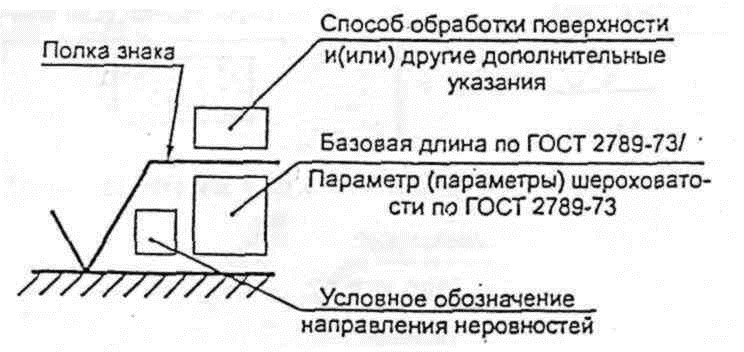
\includegraphics[width=0.6\textwidth]{3sher.png}
		\label{pic:3sher}
	\end{figure}
	
	Рабочие (оптические) преломляющие и отражающие поверхности большинства деталей (за исключением, например, матовых стекол, экранов) полируются до высоты неровностей профиля по параметру $R_z$, равному 0,05~мкм.
	
	Нерабочие поверхности могут иметь различные значения параметров шероховатости, зависящие от их назначения, свойств материалов деталей, методов их получения и обработки (литье, прессование, штамповка, резание, шлифование, полировка, травление), характеристик и зернистости обрабатывающего инструмента (абразива). Наиболее часто шероховатость таких поверхностей, достигаемая удалением слоя материала, нормируется параметром $R_a$, равным 2,5 мкм.
	
	В случаях, когда материал детали (например, бериллий, карбид кремния, титановые и алюминиевые сплавы, из которых часто изготовляют зеркала космических телескопов) не позволяет получить оптической поверхности, на нее наносят конструкционное покрытие (стеклянное, медное, никелевое), которое затем обрабатывают (полировкой, алмазным точением) для получения требуемых шероховатости и точности формы поверхности.
	
	Заметим, что оптические поверхности деталей, работающие с мощным лазерным излучением, обрабатываются с применением методов глубокого шлифования и полировки для повышения их лучевой прочности.
	
	\item Допуски на толщину (размер) оптических деталей по (вдоль) оси пучка лучей (линз, пластин, клиньев) устанавливаются обычно симметричными ($\pm$), дающими большую свободу действий оптику, по сравнению с односторонним полем допуска, так как кроме толщины детали он должен выдержать также допуск (более строгий) на точность формы рабочих поверхностей ($N$,  $\Delta N$).
	\item На силовую деталь (линзу, зеркало) устанавливают допустимое значение ее децентрировки. Под \textit{децентрировкой} понимают смещение центра(ов) кривизны ее рабочей поверхности с базовой оси детали или неперпендикулярность ее плоской рабочей поверхности к этой оси. Силовые детали (линзы, сферические и асферические зеркала, граданы) осуществляют силовое преобразование оптического излучения.  В ряде случаев (например, для цилиндрических рабочих поверхностей, деталей с некруглыми боковыми поверхностями) под децентрировкой понимают смещение или непараллельность центра кривизны либо оси цилиндра рабочей поверхности относительно базовых поверхностей.
	
	Согласно действующему стандарту (ГОСТ~2.412-81), децентрировка задается следующим образом: позиционным допуском, допуском формы заданной поверхности, перпендикулярностью (биением) плоской поверхности.
	
	Расчет допустимых значений децентрировки осуществляется исходя из допустимых значений вызываемых ею дефектов (смещения изображения, аберраций: комы, дисторсии, поперечного хроматизма) и соответствующих коэффициентов влияний децентрировок поверхностей на эти дефекты.
	\item На кромках оптических деталей, как правило, наносят фаски. Фаски подразделяют на:
	\begin{itemize}
		\item защитные (технологические), служащие для удаления микротрещин и выколок, появившихся в процессе обработки детали, предохраняющие ее от возможных сколов, трещин и разрушений при закреплении и эксплуатации из-за больших напряжений в этих дефектах под действием различных сил, а также для исключения травм персонала при изготовлении и сборке деталей из-за острых кромок и заусенцев;
		\item конструктивные, служащие для удаления излишков стекла или для базирования детали (центрировка, обеспечение воздушных промежутков между деталями) по плоской, П-образной, конической, сферической формам буртика;
		\item для крепления завальцовкой (закаткой), приклеиванием, планками.
	\end{itemize}
	
	Защитные фаски и фаски для крепления завальцовкой нормализованы для круглых оптических деталей. Размер (ширина) фаски зависит от диаметра детали, от того на склеиваемую или несклеиваемую сторону она наносится, а угол наклона фаски зависит от отношения ее диаметра $D$ к радиусу $R$.
	
	Размер защитных фасок на углах и ребрах некруглых оптических деталей (например, призм) устанавливают в зависимости от длины наиболее короткого ребра. Фаски наносят перпендикулярно биссектрисам трехгранных или двухгранных углов.
	
	\item На преломляющие и отражающие рабочие поверхности оптических деталей обычно наносят оптические покрытия -- тонкие пленки различных веществ: металлов, окислов металлов, диэлектриков, полимерных соединений, кремнийорганических соединений.
	
	Оптические покрытия позволяют изменять оптические характеристики деталей, придавать им новые физические и химические свойства. В зависимости от назначения покрытия подразделяются на следующие группы:
	\begin{itemize}
		\item просветляющие, зеркальные светоделительные, поглощающие (они изменяют интенсивность проходящего и отраженного излучения);
		\item фильтрующие, поляризующие, спектроделителъные (изменяющие спектральный состав, состояние поляризации и фазовые характеристики излучения);
		\item электропроводящие и защитные (они предназначены для обогрева деталей временной и постоянной защиты деталей, изготовленных из химически- и влагонестойких оптических материалов, для гидрофобной и фунгицидной защиты деталей, работающих в условиях морского и тропического климата, а также абразивной защиты недостаточно прочных материалов). Условные обозначения видов покрытий на чертежах оптических деталей указываются в соответствии с ГОСТ~2.412-81. 
	\end{itemize}
	
	Покрытия могут быть одно-, двух-, трех- и многослойные. На чертеже оптической детали, на контуре поверхности ставят условное графическое обозначение покрытия, а на поле чертежа, в технических условиях, после условного графического знака типа покрытия указывают сведения о покрытии.

\end{enumerate}

\section{Оформление оптических схем}

Оформление оптических схем согласно ГОСТ~2.412-81 должно выполняться в соответствии со следующими требованиями:
\begin{enumerate}
	\item На оптических схемах детали и узлы, как правило, следует располагать по ходу светового луча, идущего от плоскости предметов слева направо. 
	\item Для сложных приборов оптическую схему основной части прибора и оптические схемы узлов прибора, имеющих самостоятельное назначение, допускается  оформлять отдельными чертежами. На основной схеме такие узлы допускается обводить штрихпунктирной линией.
	\item Все движущиеся детали (вращающиеся или перемещающиеся вдоль или перпендикулярно к оптической оси системы) следует изображать в основном рабочем положении. При необходимости другие положения подвижной детали(например, крайние) могут быть показаны штрихпунктирной линией.
	\item На оптической схеме следует указывать:
	\begin{itemize}
		\item апертурные диафрагмы и положения зрачков;
		\item положения фокальных плоскостей, плоскостей изображения или предмета, положение полевой диафрагмы;
		\item источники света (схематически);
		\item приемники лучистой энергии (схематически или условными графическими обозначениями);
		\item основные оптические характеристики системы в зависимости от типа, при необходимости -- с допусками (увеличение, угловое поле, удаление выходного зрачка, относительное отверстие, предел разрешения, коэффициент светопропускания);
		\item mразличные дополнительные сведения, например расстояние от последней поверхности фотообъектива до плоскости изображения, линейное перемещение окуляра на 1 дптр, при необходимости -- типы и размеры фотокатодов и ПЗС-матриц;
		\item диаметры диафрагмы и размеры зрачков, размеры тела накала или иных светящихся элементов источников света;
		\item воздушные промежутки и другие размеры по оптической оси;
		\item размеры, определяющие пределы перемещения или предельные углы поворота подвижных оптических деталей;
		\item размеры, определяющие положение оптической системы относительно механической части прибора, например размер, определяющий положение объектива микроскопа относительно нижнего среза тубуса;
		\item габаритные или сборочные размеры, например длину базы, высоту выноса (при необходимости).
	\end{itemize}
	\item В таблицах на оптической схеме указывают:
	\begin{itemize}
		\item фокусные расстояния и фокальные отрезки отдельных узлов оптической системы, которые помещают в поле чертежа в виде таблицы;
		\item  размеры световых диаметров оптических деталей и соответствующих им стрелок прогиба ($ sag = R^2 - \sqrt{(R^2 - \dfrac{D^2_\text{св}}{4})} $, где $ R $ -- радиус кривизны поверхности, $ D $ -- световой диаметр), а также толщину по оси (для призм -- длину развертки), которые помещают в поле чертежа в виде таблицы; 
		\item спецификацию -- перечень деталей, входящих в состав оптической схемы с указанием позиции(формат спецификации стандартный), формата и номера чертежа, количества и названия деталей; 
		располагается эта таблица над основной надписью оптической схемы.
		\end{itemize}
\end{enumerate}

Пример оформления оптической схемы представлен на рис.~\ref{pic:3OS}. Пример оформления схемы комбинированной принципиальной показан на рис.~\ref{pic:3Comb}.

\begin{figure}[H]
	\caption{Оптическая схема оптико-электронного преобразователя}
	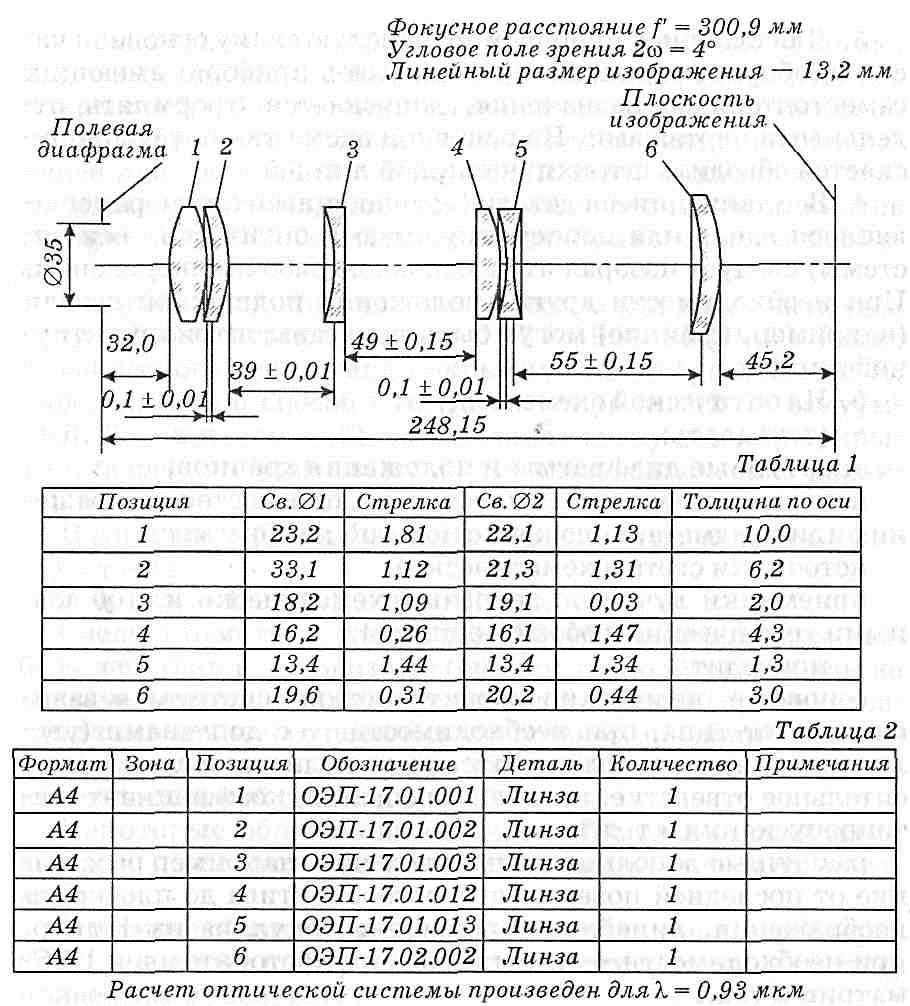
\includegraphics[width=1\textwidth]{3OS.png}
	\label{pic:3OS}
\end{figure}

\begin{landscape}
	\begin{figure}[h!]
		\caption{Схема комбинированная принципиальная}
		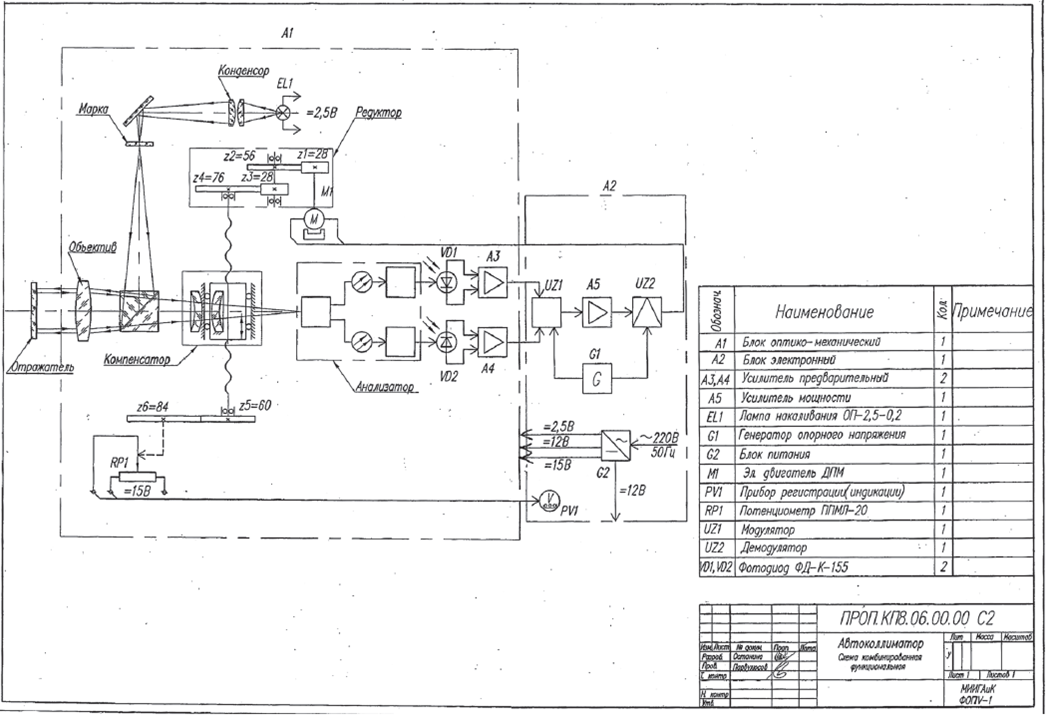
\includegraphics[width=0.9\textwidth]{3Comb.png}
		\label{pic:3Comb}
	\end{figure}
\end{landscape}

%\chapter[Основные принципы, правила и методы конструирования деталей и\\ функциональных устройств ОЭП]{Основные принципы, правила и методы конструирования деталей и функциональных устройств ОЭП}

\section{Принципы конструирования деталей}

\begin{flushleft}
	\textbf{Общие аспекты конструирования деталей}
\end{flushleft}

Рассмотрим кратко некоторые общие, а также специфические вопросы конструирования деталей. 

\textit{Детали} являются простейшими объектами конструирования и представляют собой неделимые однородные тела, состоящие из элементов формы (геометрических поверхностей тел) и материала.

В каждой детали различают следующие структурные элементы (поверхности): рабочие (активные), базовые, соединительные (свободные) и технологические.

\textit{Рабочие элементы} (РЭ -- их называют также активными или исполнительными поверхностями) непосредственно выполняют заданные функции детали. Например, РЭ являются: сферические поверхности линзы (рис.~\ref{pic:4det}~а); эвольвентная поверхность зубчатого венца колеса (рис.~\ref{pic:4det}~б); плоская и цилиндрическая поверхности гнезда оправы линзы (рис.~\ref{pic:4det}~в). Эти поверхности, как правило, тщательно обрабатываются, и к ним предъявляются высокие требования: точность расположения, погрешность формы, чистота поверхности, размеры.

\textit{Базовые элементы} (БЭ) обеспечивают координацию детали (т. е. координацию ее РЭ) относительно других деталей и представляют собой поверхности, по которым деталь сопрягается (соединяется) с базовой деталью (рис.~\ref{pic:4det}). Данные поверхности изготавливаются также весьма тщательно.

\textit{Соединительные элементы} (СЭ -- их называют часто свободными) служат для обеспечения материальной связи между рабочими и базовыми элементами (рис.~\ref{pic:4det}). К СЭ не предъявляются высокие требования по тщательности и точности изготовления (за исключением требований к чистоте поверхностей, когда это обусловлено эстетическими показателями качества детали).

\begin{figure}[H]
	\caption{Структурные элементы деталей}
	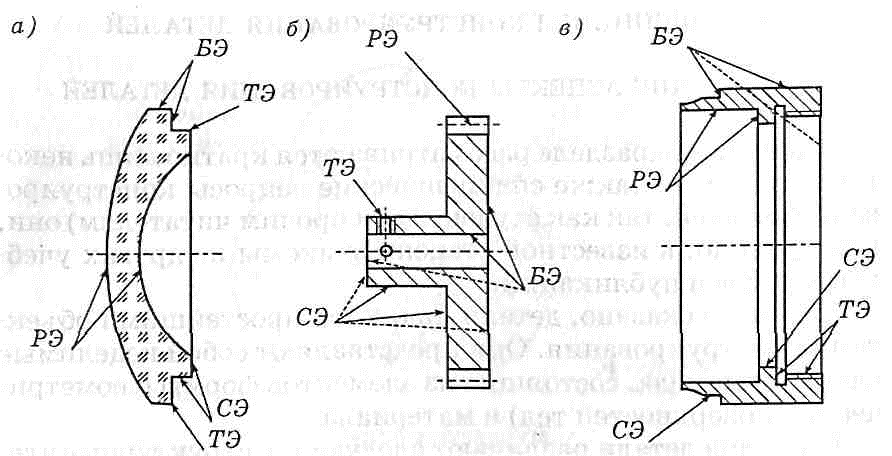
\includegraphics[width=1\textwidth]{4det.png}
	\label{pic:4det}
\end{figure}

\textit{Технологические элементы} (ТЭ) служат для обеспечения технологического процесса изготовления и последующей сборки детали (например, фаски, галтели, выточки, центровые отверстия в валиках). Для линзы (рис.~\ref{pic:4det}~а) ТЭ являются фаски, которые устраняют выколки, появляющиеся на кромках при ее шлифовке; для зубчатого колеса (рис.~\ref{pic:4det}~б) ТЭ является резьбовое отверстие под стопорный винт для фиксации зубчатого колеса на валике при рассверливании отверстия под штифт; в оправе линзы (рис.~\ref{pic:4det}~в) ТЭ является резьба (и канавка для выхода резьбы) для закрепления оправы (с линзой) в центрировочном патроне для результативной обработки ее базовых поверхностей в размер.

Следует отметить, что одни и те же поверхности (части поверхностей) могут выполнять роль РЭ, БЭ и СЭ. Наиболее благоприятным считается вариант, когда в конструкции удается объединить РЭ и БЭ, минимизировать СЭ.

Конструирование детали заключается в выборе материала, формы ее поверхностей и определения ее размеров. Кроме этого, конструктор должен указать допустимые отклонения характеристик материала, погрешности изготовления размеров и форм, тип покрытий, вид обработки, технические и технологические условия и требования (например, азотирование, просветление, старение).

Выбор материала производится исходя из функционального назначения детали, условий ее эксплуатации, рациональной технологии изготовления, стоимости и дефицитности материала, требований эргономики и эстетики.

Конструктор руководствуется при этом номенклатурой и физико-механическими свойствами конструкционных материалов (табл.~\ref{tab:prop}).

\begin{table}[h]
	\caption{Физико-механические и технологические свойства материалов}
	\label{tab:prop}
	\begin{tabular}{|c|c|} \hline 
		Свойства & Характеристики \\ \hline
		\multirow{5}{*}{Механические} & Плотность\\ 
		& Упругость \\ 
		& Твердость \\
		& Износотойкость \\
		& Прочность\\ \hline
		\multirow{5}{*}{Тепловые} & Коэффициент линейного расширения\\
		& Теплопроводность \\
		& Теплоемкость \\
		& Термооптические постоянные \\
		& Термостойкость \\ \hline
        \multirow{4}{*}{Химические, коррозионные} & Налетоопасность \\
        & Радиационная устойчивость \\
        & Коррозионная стойкость \\
        & Водопоглощаемость (влагостойкость)\\ \hline
        \multirow{3}{*}{Электромагнитные} & Удельное электрическое сопротивление \\
        & Магнитная проницаемость \\
        & Пробивная электрическая прочность\\ \hline
        \multirow{4}{*}{Фрикционные} & Коэффициент трения скольжения \\
        & Коэффициент трения качения \\
        & Коэффициент сцепления \\ \hline
        \multirow{4}{*}{Технологические}  & Пластичность \\
        & Свариваемость \\
        & Прессуемость \\
        & Трудоемкость обработки \\ \hline
	\end{tabular}
\end{table}

Например, если конструируется линза, то ее материал должен быть прозрачным для рабочего диапазона длин волн света. Если линза будет эксплуатироваться в условиях тропического или морского климата, необходимо выбрать материал, стойкий к воздействию влаги, грибков, соли и других вредных факторов. Исходя из условия минимизации массы, возможности получения линзы литьем, она могла бы быть изготовлена из органического стекла (если это не влияет на другие показатели качества детали).

Естественно, что характеристики используемого материала должны обеспечить необходимую точность размеров, форм и шероховатость (чистоту) поверхностей детали при ее изготовлении, а также сохранение их стабильными в процессе длительной эксплуатации при воздействии различных факторов.

Технологичными считаются материалы, которые легко обрабатываются резанием, шлифуются, штампуются, прессуются, свариваются, спекаются, имеют хорошие литейные свойства. Общей современной тенденцией являются использование таких материалов, из которых можно изготавливать детали производительными методами (например, литьем под давлением, штамповкой, прессованием), а также широкое применение пластмасс.

При выборе материала деталей, взаимодействующих с человеком как непосредственно, так и косвенно, учитываются эргономические показатели: гигиенические, антропометрические и психофизиологические (уровень шума, амплитуда и частота вибраций, температура, возможность получения оптимальной формы, усилия, контраст, класс исполнения, степень утилизации). Например, такой перспективный для изготовления космических зеркал материал, как бериллий, обладающий для этого рядом очень хороших характеристик, является весьма токсичным при обработке, что ограничивает его использование.

Свойство материала обуславливает также достижение соответствия формы внешних деталей их назначению, качество и совершенство отделки, возможность нанесения декоративных покрытий и другие эстетические показатели.

В общем случае решение задачи по выбору материала детали является многовариантным, так как требования к точности, надежности, массе, прочности, жесткости, экономичности, эстетичности и др. вступают в противоречие друг с другом, которое приходится преодолевать, оптимизируя выбор материала с помощью ранжирования значимости показателей качества детали и свойств материала. Весьма часто выбор материала производится с помощью расчета необходимых значений некоторых его характеристик по требуемым показателям качества (например, марок и оптических констант стекла по допустимым аберрациям системы, модуля упругости материала валика по его допустимым деформациям, коэффициента линейного расширения материала по допустимым изменениям размеров детали при изменении температуры).

Конструктор должен постоянно следить за появлением новых материалов, а также пытаться использовать нетрадиционные (для ответственных деталей) материалы, которые благодаря своим свойствам могут повысить показатели качества проектируемого изделия.

Выбор формы ограничивающих деталь поверхностей осуществляют исходя из их структуры (функционального назначения), технологичности, эстетических и эргономических требований, конструктивной целесообразности. Форма рабочих элементов типовых деталей часто бывает вполне определенной. Примерами могут служить сферические поверхности линз, плоские поверхности преломляющих и отражающих граней призм, эвольвентные поверхности зубьев зубчатого колеса, спиральный профиль кулачка.

Рабочие элементы оригинальных деталей выполняют в виде специальных поверхностей, например параболическими, эллиптическими, торическими. Форма базовых, свободных и технологических элементов обычно представляет собой типовые поверхности -- плоскость, цилиндр, конус, сферу -- для оптических. Более технологичными являются типовые поверхности, получаемые при обработке деталей на универсальном оборудовании типовым инструментом.

Параметры формы могут быть получены эвристически, расчетным путем, исходя из условий стандартизации и унификации, технологических возможностей производства (например, радиусы кривизны сферических поверхностей линз определяют из аберрационного расчета и ГОСТов на них, угол конуса конической или дугообразной поверхности центрового отверстия детали назначают исходя из типа детали, ее массы, требований к точности обработки и ГОСТ~14034-74).

Определение размеров детали производится с учетом большого числа факторов, среди которых следует выделить функциональную точность, параметрическую надежность, жесткость, компактность, эстетичность и эргономичность, технологичность, требования стандартизации и унификации, массу и используемые материалы. Конструктор, руководствуясь вышеперечисленными факторами, выбирает или рассчитывает необходимые размеры структурных элементов детали.

В наиболее ответственных случаях детали подвергаются тщательному расчету (а иногда и экспериментальным исследованиям) по математическим моделям, связывающим ее размеры (и параметры формы) с требуемыми показателями качества, компоновкой, условиями эксплуатации, производства и другими ограничениями. Как правило, это детали, определяющие точность функционирования, качество создаваемого изображения, испытывающие значительные статические, динамические, тепловые нагрузки (например, детали астрономических, военных, космических приборов).

Для оптических деталей подобными расчетами (например, габаритно-аберрационным) определяют размеры и расположение рабочих элементов. Весьма важный аспект конструирования детали -- это обеспечение технологичности ее конструкции (ГОСТ~14.204-73), значимой характеристикой которой является трудоемкость изготовления и в дальнейшем сборки детали.

Трудоемкость изготовления детали зависит от рациональности выбранного материала и оптимальности ее форм и размеров для условий современного производства. 

При конструировании деталей конструктор должен определить способ термообработки, тип покрытий и смазочный материал, которые оказывают существенное влияние на показатели их назначения и особенно надежности.

Благодаря термообработке (закалке, отжигу, старению) улучшаются, например, характеристики прочности и твердости, износостойкости, снижаются остаточные напряжения (вызывающие их деформацию во времени), появляется возможность получения более точных поверхностей в деталях.

Покрытия деталей позволяют защитить их от коррозии (налетоопасности, пятнаемости), улучшить их внешний вид, уменьшить износостойкость, изменить некоторые характеристики (например, теплопроводность, электрическое сопротивление, коэффициент отражения).

Особенно широко применяются покрытия оптических деталей: просветляющие, зеркальные, поляризующие, токопроводящие, покрытия-фильтры, защитные.
Смазочные материалы, (замазки) предназначены для уменьшения трения и износа подвижных деталей, защиты от коррозии, герметизации и влаго- и пылезащиты.

Вопросы термообработки, покрытий, смазки деталей точных приборов изложены в соответствующих справочниках, ГОСТах и специальной литературе.

\begin{flushleft}
\textbf{Принцип совместной обработки рабочих и базовых элементов детали}
\end{flushleft}

Этот принцип заключается в предпочтительности конструкции детали, позволяющей осуществлять совместную технологическую обработку (за одну установку) ее рабочих и базовых элементов, так как в этом случае точность их взаимного расположения будет выше.

На рис.~\ref{pic:4oprava} изображены варианты упрощенной конструкции оправы линз объектива, в одном из которых оба рабочих элемента (РЭ$ _1 $, РЭ$ _2 $) не могут быть обработаны совместно с базовым элементом (рис.~\ref{pic:4oprava}~а), а в другом такая возможность существует (рис.~\ref{pic:4oprava}~б). В первом случае погрешность расположения РЭ$ _2 $ относительно РЭ$ _1 $ и БЭ будет больше, а следовательно, хуже центрировка линз и точность выдерживания воздушного промежутка, чем во втором варианте. Обусловлено это тем, что при перестановке (технологическом перебазировании) оправы в патроне станка возникают погрешности взаимного расположения ее РЭ и БЭ, обусловленные изменением технологической и измерительных баз.

\begin{figure}[H]
	\caption{Конструкции оправы}
	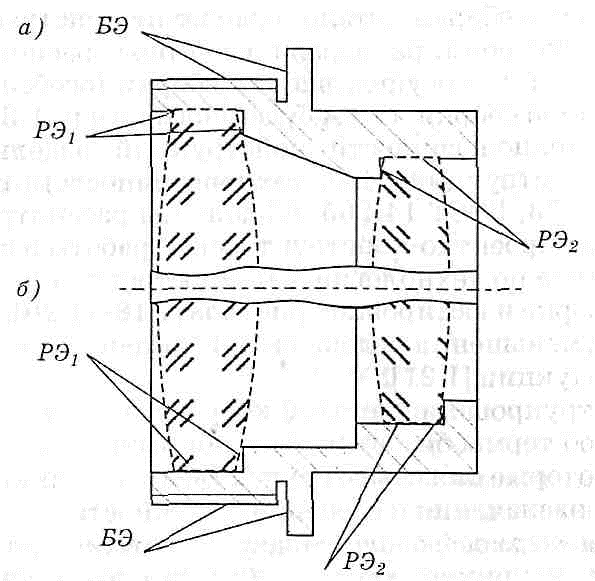
\includegraphics[width=0.4\textwidth]{4oprava.png}
	\label{pic:4oprava}
\end{figure}

\begin{flushleft}
\textbf{Принцип точностной технологичности деталей}
\end{flushleft}

Этот принцип заключается в учете экономических факторов при назначении допусков на характеристики материала детали и на погрешности ее изготовления.

Конструктор должен помнить, что от допусков на деталь в существенной степени зависит ее стоимость. Назначение высоких (жестких) допусков на погрешности изготовления деталей приводит к существенному их удорожанию, поэтому такие допуски должны быть обоснованы другими факторами, связанными, например, с затратами на сборку, точностью функционирования всего прибора. Также,  чем выше качество используемого материала, тем она дороже. Например, стоимость оптического стекла первой категории класса А по показателю преломления и средней дисперсии в несколько раз больше, чем стекло той же марки пятой категории класса Г, а его стоимость с учетом всех показателей качества может отличаться на порядок.

\section{Принципы конструирования соединений}

\textit{Соединением деталей} в конструкторском смысле (как элемента конструкции) называют конструкцию элементарной сборочной единицы, которая состоит из двух или нескольких деталей, находящихся в непосредственном контакте (сопряжении) друг с другом. 

\textit{Соединением деталей} в технологическом смысле (как сборочную операцию) называют сопряжение деталей путем их сочленения, свинчивания, развальцовки, сварки

Соединяемые детали образуют контактные пары, которые классифицируют как: подвижные и неподвижные; замыкающиеся формой, силой и креплением; сопрягающиеся (контактирующие) по поверхности, по линии и по точке.

В соединении различают базовую и рабочую (присоединяемую) детали, а также базовые (БЭС) и рабочие (РЭС) элементы (поверхности) соединения.

На рис.~\ref{pic:4elements} показано соединение линзы (рабочая присоединяемая деталь~1) с оправой~2 (базовая деталь) с помощью резьбового кольца~3, которое является в соединении вспомогательной деталью, осуществляющей силовое замыкание линзы на торцевую посадочную поверхность оправы.

\begin{figure}[H]
	\caption{Элементы, соединения, деталей}
	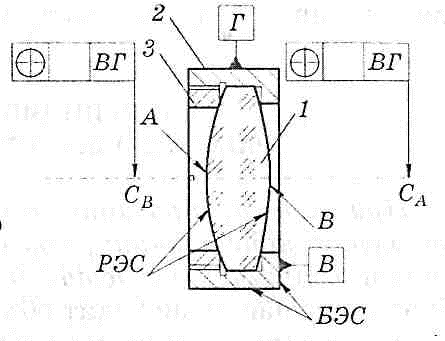
\includegraphics[width=0.6\textwidth]{4elements.png}
	\label{pic:4elements}
\end{figure}

Показатели качества соединений подразделяются: на эксплуатационные (точность, надежность, износостойкость, несущая способность); конструктивные (габаритные размеры, масса, компактность); технологические (технологичность сборки, юстировки и контроля).

Конструируя соединения, в первую очередь стараются достичь их точности (характеризуемой погрешностью расположения РЭС относительно БЭС, рис.~\ref{pic:4elements}), надежности и технологичности.

Рассмотрим принципы конструирования соединений, позволяющие обеспечить эти показатели, основанные на общих правилах и законах наложения материальных связей деталей друг на друга в соединении.

\begin{flushleft}
\textbf{Принцип совмещения рабочих элементов в соединении}
\end{flushleft}

При конструировании соединений предпочтительной является конструкция, позволяющая осуществлять контакт сопрягаемых деталей по их рабочим элементам. В этом случае происходит объединение рабочего и базового элементов присоединяемой детали, уменьшается размерная цепь и повышается точность расположения РЭС относительно БЭС.

На рис.~\ref{pic:4mirror} изображена конструкция соединения зеркала 1 с кронштейном 2. Конструкция, изображенная на рис.~\ref{pic:4mirror}~б, позволяет точнее ориентировать отражающую поверхность зеркала (РЭС) относительно основания кронштейна (БЭС) и не требует жесткого допуска на клиновидность зеркала по сравнению с конструкцией, изображенной на рис.~\ref{pic:4mirror}~а.

\begin{figure}[H]
	\caption{Соединение зеркала с оправой}
	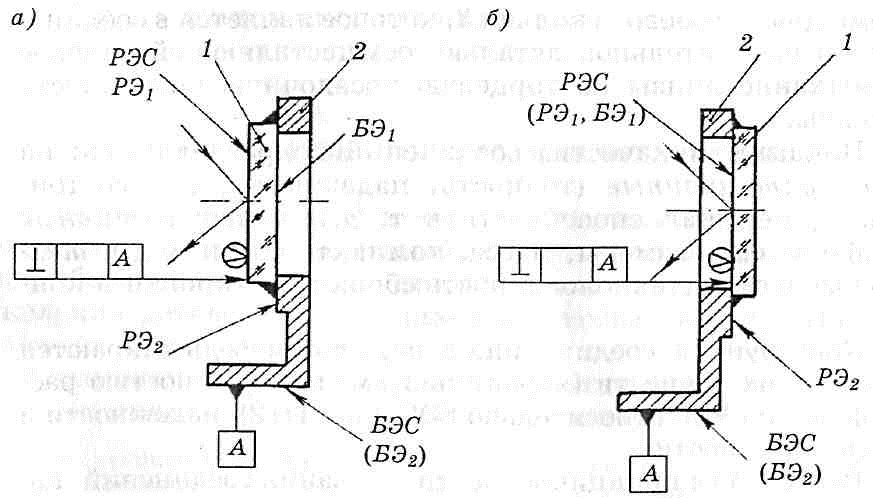
\includegraphics[width=0.7\textwidth]{4mirror.png}
	\label{pic:4mirror}
\end{figure}

\begin{flushleft}
\textbf{Принцип отсутствия избыточного базирования в соединении деталей -- статическая определенность соединений}
\end{flushleft}

Придание материальным телам определенного и строго фиксированного положения в пространстве называют базированием. При базировании происходит отнятие лишних степеней свободы присоединяемой детали относительно базовой в их соединении.

Базирование называют избыточным, когда лишние степени свободы присоединяемой детали отняты более одного раза, т.е. когда для отнятия лишней степени свободы наложена более чем одна связь. Соотношение между оставшимися степенями свободы $n$ и числом наложенных связей $ m $ должно быть $ n+m = 6 $.

В некоторых случаях нарушение принципа можно видеть невооруженным глазом~-- по дублированию сопряжений деталей (базовых элементов), отнимающих одни и те же степени свободы у присоединяемой детали относительно базовой (рис.~\ref{pic:4double}~а).

Устранить неопределенность базирования можно изменив конструкцию сопряжения деталей (рис.~\ref{pic:4double}~б). 

\begin{figure}[H]
	\caption{Дублирование в сопряжении деталей}
	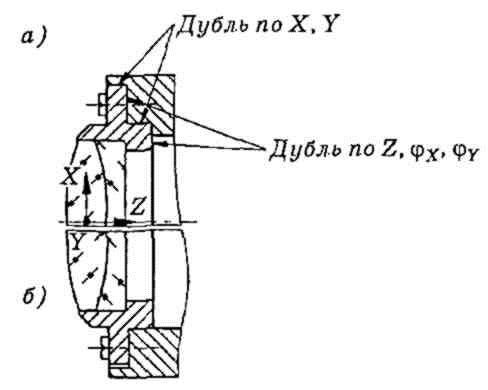
\includegraphics[width=0.6\textwidth]{4double.png}
	\label{pic:4double}
\end{figure}

\begin{flushleft}
\textbf{Принцип геометрической определенности контакта пар в соединении}
\end{flushleft}

Этот принцип заключается в определенности положения и формы, контакта сопрягаемых поверхностей деталей. Реальные поверхности деталей имеют макро- и микропогрешности формы поверхностей. В результате детали контактируют друг с другом не по линиям и поверхностям, а по пятнам (площадкам) неопределенной формы, размеры и положения которых в сопряжении также неопределенны.

Эта неопределенность снижает точность расположения присоединяемой детали и несущую способность базовой детали. Наибольшее влияние на точность оказывает неопределенность расположения пятен контакта.

На рис.~\ref{pic:4connect}~а изображено соединение зеркала~1 с оправой~2 с помощью трех угольников. Из-за погрешностей формы сопрягаемых поверхностей зеркала и оправы их контакт будет происходить не по плоскости, а по трем площадкам 3, расположение и форма которых могут быть произвольными в пределах сопрягаемых поверхностей. В результате возникает объемная деформация зеркала под действием сил $ F $ со стороны угольников и реакции $ R $ со стороны оправы, приводящая к порче качества изображения.

Соединение, изображенное на рис.~\ref{pic:4connect}~б, обладает определенностью расположения площадок контакта благодаря специальным выборкам (либо прокладкам) на оправе. Здесь возникает только контактная деформация зеркала в пределах контактирующих зон, не приводящая к ухудшению качества изображения.

\begin{figure}[H]
	\caption{Сопряжение зеркала с оправой}
	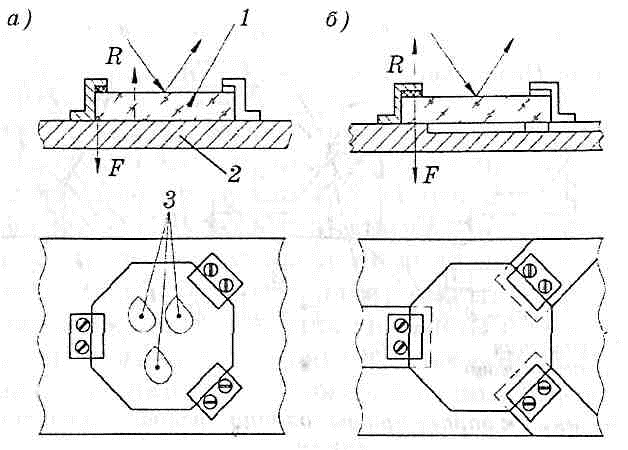
\includegraphics[width=0.85\textwidth]{4connect.png}
	\label{pic:4connect}
\end{figure}

\begin{flushleft}
\textbf{Принцип силового замыкания}
\end{flushleft}

Силовое замыкание соединений следует осуществлять так, чтобы линия действия замыкающей силы проходила через зону (площадку) контакта сопрягаемых поверхностей. Тогда сила и возникающая реакция не образуют изгибающего момента, действующего на присоединяемую и базовые детали. Примерами выполнения этого принципа могут служить рассмотренное крепление зеркала (рис.~\ref{pic:4connect}~б).

\begin{flushleft}
\textbf{Принцип ограничения смещений в соединении деталей}
\end{flushleft}

Согласно этому принципу поверхности, ограничивающие смещение присоединяемой детали относительно базовой, следует располагать перпендикулярно к направлению ограничиваемого смещения.

В этом случае более точно обеспечивается расположение рабочих элементов соединения относительно базовых, более благоприятным будет силовой режим в соединении (связанный с деформациями деталей, их износом), технологичнее будут детали.

\begin{flushleft}
\textbf{Принцип ограничения поворотов}
\end{flushleft}

Согласно этому принципу связи, накладываемые базовой деталью на присоединяемую, должны располагаться на возможно большем базисе. Тогда погрешность углового положения присоединяемой детали при прочих равных условиях будет наименьшей.

На рис.~\ref{pic:4axe} изображены схемы конструкций соединения вала~1 с подшипниками~2 для поворота зеркала вокруг оси $ Y $. Вариант, показанный на рис.~\ref{pic:4axe}~а, уступает варианту, изображенному на рис.~\ref{pic:4axe}~б, так как база $ B_1 $ между подшипниками, ограничивающая возможные повороты вала относительно осей $ Z, X $ (например, из-за биений   внутренних колец подшипников  ), меньше базы $ B_2 $ при одном и том же габаритном размере $ L $ конструкции.

\begin{figure}[H]
	\caption{Осевая система зеркала}
	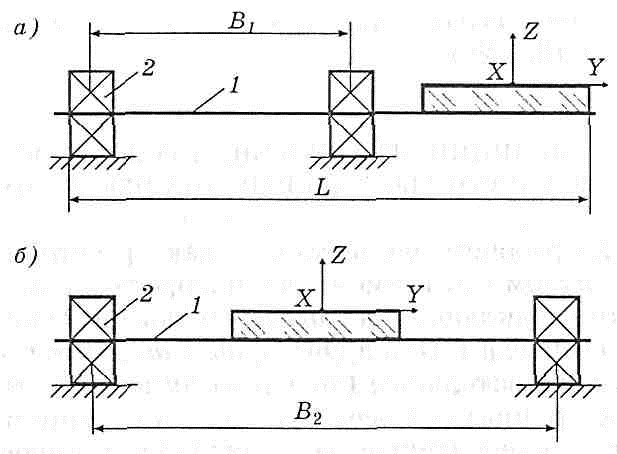
\includegraphics[width=0.6\textwidth]{4axe.png}
	\label{pic:4axe}
\end{figure}

\begin{flushleft}
\textbf{Принцип ограничения продольного и поперечного вылетов рабочих элементов}
\end{flushleft}

<<Вылетом>> рабочего элемента называют расстояние между ним и центром его возможного поворота в соединении. Суть принципа заключается в ограничении продольного или поперечного (иногда того и другого) вылетов, что позволяет уменьшить нежелательные (опасные) линейные смещения РЭС вдоль координатных осей при возникновении поворота рабочей детали относительно базовых элементов соединения из-за погрешностей формы сопрягаемых поверхностей, деформаций, зазоров.

Базирование оправы линзы (рис.~\ref{pic:4connlens}) в кронштейне, устанавливаемом на рейтере, приводит к тому, что узловая точка линзы (РЭС) имеет поперечный $ H $ и может иметь продольный $ L $ вылеты относительно возможного центра поворота оправы $ C $. В результате при повороте оправы на угол $ \Delta\gamma $  РЭС имеет смещение (расфокусировку) вдоль оси $ Z $ ( $ \Delta Z_{\Delta\gamma} \approx H\Delta\gamma$ ) и децентрировку вдоль оси $ X $ ( $ \Delta X_{\Delta\gamma} = L\Delta\gamma $ ). Штриховой линией на этом рисунке изображена конструкция кронштейна, позволяющая ограничить вылет $ L $.

\begin{figure}[h!]
	\caption{Сопряжение оправ линзовых систем с корпусной деталью}
	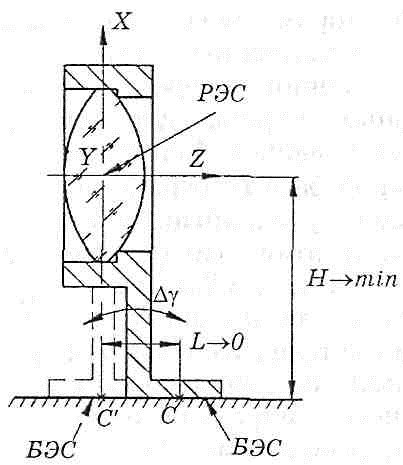
\includegraphics[width=0.4\textwidth]{4connlens.png}
	\label{pic:4connlens}
\end{figure}

\begin{flushleft}
\textbf{Учет тепловых свойств соединяемых деталей}
\end{flushleft}

Этот принцип заключается в обеспечении отсутствия возможных деформаций и смещений сопрягаемых деталей в соединении при отклонении температуры, от номинального значения.

Чаще всего указанные дефекты возникают из-за разности коэффициентов линейного расширения материалов базовой и присоединяемой деталей. Для соблюдения принципа следует обеспечить возможность относительного изменения размеров деталей (при отклонении температуры) без нарушения их взаимного базирования благодаря выбору соответствующих зазоров в посадке, упругому силовому замыканию, целенаправленному подбору материалов и размеров деталей, применяя термокомпенсаторы.

Рассмотрим типовое соединение линзы с оправой с помощью резьбового кольца (рис.~\ref{pic:4opt}~а).
\begin{figure}[H]
	\caption{Крепление оптических деталей в оправах}
	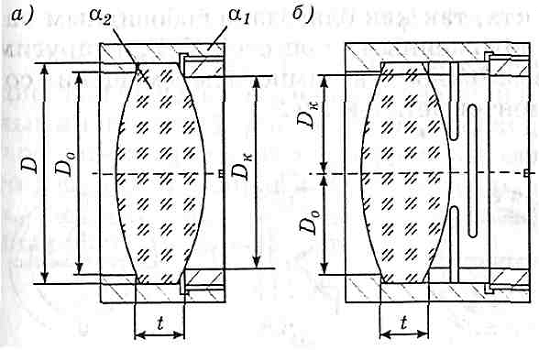
\includegraphics[width=0.6\textwidth]{4opt.png}
	\label{pic:4opt}
\end{figure}

Когда коэффициенты линейного расширения материалов оправы $ \alpha_1 $ и линзы $ \alpha_2 $ различны, отклонение температуры от номинального значения приводит к изменению диаметров $ D $ линзы и оправы, диаметров $ D_0, D_K $, размера $ t $. Это может вызвать либо деформацию линзы (и оправы), либо смещение линзы в зазоре. Например, когда посадка линзы в оправу по диаметру $ D $ обеспечивает необходимый температурный зазор, деформация или зазор возникают из-за несоответствия изменений $ D_0 $ и $ t $ линзы и оправы. Пружинное кольцо, помещенное между линзой и резьбовым кольцом (рис.~\ref{pic:4opt}~б), позволяет избежать указанных недостатков (при достаточном температурном зазоре в посадке), так как компенсирует осевое изменение размеров линзы и оправы, а также изменение диаметров $ D_0, D_K $.

\begin{flushleft}
\textbf{Точностная технологичность соединений}
\end{flushleft}

В процессе сборки детали соединяются путем сочленения, свинчивания, завальцовки или склейки.

Технологичность соединения определяется трудоемкостью сборки, трудоемкостью контроля качества сборки, уровнем необходимой квалификации персонала.
Наиболее технологичными являются соединения, которые могут быть собраны с использованием автоматического оборудования и промышленных роботов. Поэтому конструктор должен руководствоваться не только рассмотренными общими принципами конструирования соединений (выполнение которых, как правило, повышает их технологичность), но и частными правилами, касающимися автоматизации сборочных операций. Эти правила заключаются:
\begin{enumerate}
	\item в обеспечении полной взаимозаменяемости деталей;
	\item стремлении к симметрии относительно наибольшего числа осей;
	\item минимизации числа соединительных элементов;
	\item исключении одновременного начала контактирования сопрягаемых деталей по нескольким поверхностям;
	\item осуществлении центрирования с помощью вращательно-симметричных деталей;
	\item предотвращении кинематически сложного движения рабочей детали в положение для сборки с базовой.
\end{enumerate}

Одно из основных требований к качеству соединений~-- точность расположения их рабочих элементов относительно базовых (рис.~\ref{pic:4elements}). Оно достигается благодаря точному изготовлению соответствующих элементов сопрягаемых деталей, а также с помощью их доводок и регулировок (юстировок) в соединении. Получаемую при этом точность соединений можно отнести к группам пониженной, средней и высокой точности, которые по соответствующей трудоемкости их достижения называют часто экономическим, производственным, и техническим, уровнями точности сборки деталей.

\textit{Экономическому уровню} соответствует точность, достигаемая при сборке деталей без последующих пригонок и регулировок. Точность расположения рабочих элементов соединения относительно базовых при этом определяется погрешностями изготовления и сборки соответствующих элементов сопрягаемых деталей.

\textit{Производственному уровню} соответствует точность, достигаемая при сборке с применением пригонки, регулировки и универсального оборудования и инструмента, и контролем на качественном уровне либо простейшими контрольными и измерительными средствами (индикаторами, калибрами, уровнями, шаблонами).

Точность соединения тогда будет выше, так как часть погрешностей деталей компенсируется. Естественно, трудоемкость этой сборки будет выше.

\textit{Техническому уровню} соответствует точность, достигаемая при сборке с пригонками, регулировками и доводками и контроле с помощью прецизионных средств (автоколлиматоров, микроскопов, интерферометров), а также обеспечением соответствующих условий производства (стабилизации температуры, защиты от вибраций, чистоты рабочих мест).

\section{Принципы конструирования узлов и функциональных устройств ОЭП}

Узлы и функциональные устройства (ФУ) представляют собой более сложные, чем соединения, сборочные единицы, состоящие из большего числа деталей и элементов, которые могут выполнить совместно с другими составными частями ОЭП (или самостоятельно) определенную функцию. Это, например, объективы, окуляры, механизмы, сканирующие устройства, устройства крепления источников и приемников излучения, затворы, диафрагмы, столики, датчики. В узлах и ФУ целесообразно различать рабочие (исполнительные), базовые (несущие) и эталонные (образцовые) детали и рабочие (РЭУ), базовые (БЭУ) и эталонные (ЭЭУ) элементы устройств.

Основные показатели качества узлов и ФУ -- точность (расположения РЭУ относительно БЭУ и ЭЭУ) передачи и преобразования информации, качество создаваемого изображения, надежность и технологичность.

Рассматриваемые далее принципы заключаются в общих правилах конструирования механических и оптических ФУ прибора, позволяющих оптимизировать их структуру, внутренние связи и взаимодействие элементов в целях повышения упомянутых показателей качества создаваемых ФУ.

\begin{flushleft}
\textbf{Принцип АББЕ}
\end{flushleft}

По этому принципу, называемому также принципом исключения компараторной погрешности, эталонный элемент устройства должен быть расположен соосно с рабочим, элементом (или измеряемым объектом). В этом случае уменьшается погрешность взаимного линейного расположения эталонного и рабочего элементов при возникновении поворотов деталей из-за технологических или эксплуатационных погрешностей (зазоров, погрешностей формы контактирующих поверхностей, деформаций, биений).

На рис.~\ref{pic:4comparator} показан классический пример, давший второе название принципу с поперечным (рис.~\ref{pic:4comparator}~а) и продольным (рис.~\ref{pic:4comparator}~б) компараторами.
\begin{figure}[h!]
	\caption{Компараторы}
	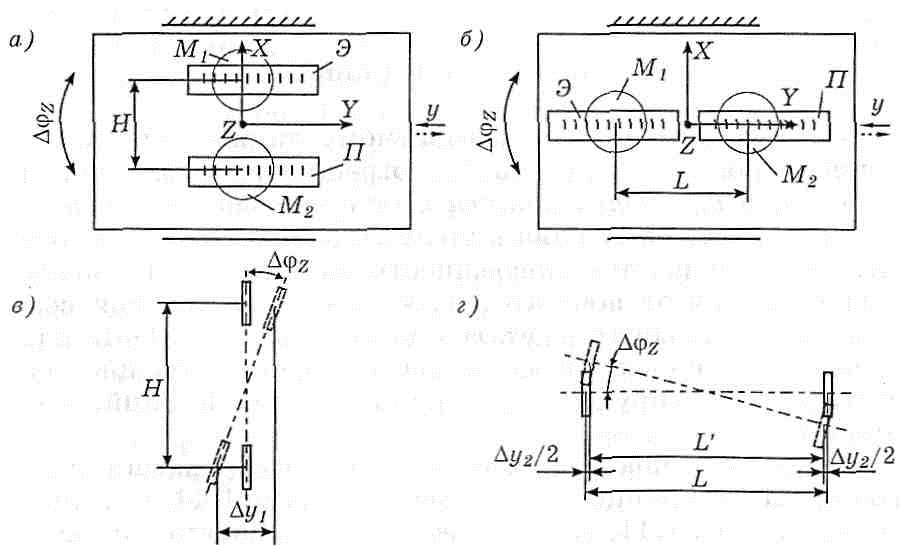
\includegraphics[width=1\textwidth]{4comparator.png}
	\label{pic:4comparator}
\end{figure}

На каретке, перемещаемой вдоль оси $ Y $, установлены эталонная Э и поверяемая П шкалы, взаимное положение штрихов которых измеряется с помощью отсчетных микроскопов $ M_1, M_2 $.

В поперечном компараторе, из-за поворотов каретки $ (\Delta \varphi_z) $ вокруг оси $ Z $, обусловленных погрешностями направляющих, возникает значительная погрешность измерения $ \Delta y_1 $ первого порядка малости, пропорциональная расстоянию $ Н $ между шкалами (рис.~\ref{pic:4comparator}~в):
\[ 
\Delta y_1 = H\,\sin\Delta\varphi_z\,\approx\, H\,\Delta\varphi_z
\]

Чтобы исключить погрешность первого порядка, Аббе предложил расположить эталонную и поверяемую шкалы соосно, преобразовав компаратор в продольный (компаратор Аббе). В этом случае погрешность измерения из-за поворотов каретки будет лишь второго порядка малости (рис.~\ref{pic:4comparator}~г):
\[ 
\Delta y_2 = L - L' = 2L\sin^2(\Delta\varphi/2) \approx L \Delta\varphi^2 /2.
\]

\begin{flushleft}
\textbf{Принцип кратчайшей цепи преобразования}
\end{flushleft}

Так же, как и кратчайшая размерная цепь (позволяющая получить более высокую точность размера замыкающего звена), кратчайшая цепь преобразования, содержащая минимальное число преобразователей, позволяет получить более высокую точность функционирования устройства благодаря меньшему числу источников погрешностей.

Сравним, например, теодолит и стереотрубу, функциональные схемы которых изображены на рис.~\ref{pic:4teodolit}.

\begin{figure}[h!]
	\caption{Функциональные схемы теодолита (а) и стереотрубы (б)}
	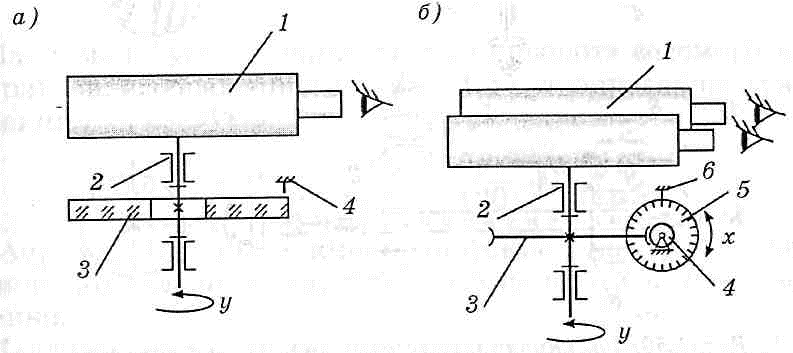
\includegraphics[width=1\textwidth]{4teodolit.png}
	\label{pic:4teodolit}
\end{figure}

Горизонтальные углы на местности измеряются теодолитом (рис.~\ref{pic:4teodolit}~а) при наведении зрительной трубы 1 на объект наблюдения (рейку) ее разворотом вокруг вертикальной оси 2 с помощью лимба 3 и индекса (отсчетной системы) 4. 

Измерения горизонтальных углов стереотрубой (рис.~\ref{pic:4teodolit}~б) осуществляются наведением зрительных труб 1 на объект их разворотом вокруг вертикальной оси 2 с помощью отсчетной червячной передачи 3, 4 и лимба 5 с индексом~6.

Теодолит, содержащий всего одну кинематическую пару (осевую систему), существенно превосходит по точности (погрешность измерения углов точными и грубыми теодолитами:  $ \Delta y=2\div30'' $) стереотрубу, кинематическая цепь которой содержит две осевые системы и отсчетную червячную передачу. 

Точность стереотруб не превосходит одной-двух минут и обуславливается главным образом кинематической погрешностью червячной передачи.

\begin{flushleft}
\textbf{Принцип наибольших масштабов преобразования}
\end{flushleft}

Согласно этому принципу функциональные элементы, осуществляющие наибольший масштаб преобразования, следует ставить в конце (для устройств, работающих на редукцию) либо в начале (для устройств, работающих на мультипликацию) цепи элементарных преобразователей, а также необходимо соотносить масштаб преобразования с погрешностями элементов. В этом случае суммарная погрешность устройства будет ниже.

\begin{figure}[H]
	\caption{Кинетические схемы, приводов}
	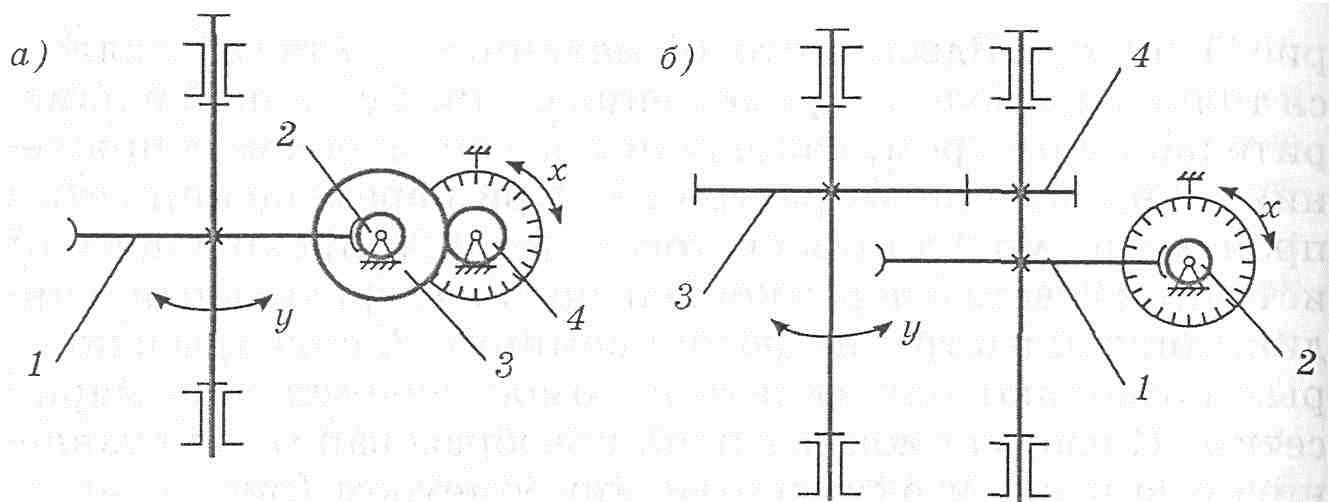
\includegraphics[width=1\textwidth]{4kinetic.png}
	\label{pic:4kinetic}
\end{figure}

На рис.~\ref{pic:4kinetic} показаны две схемы отсчетных приборов углоизмерительной бабки (стола). Оба привода состоят из одинаковых червячных 1, 2 и зубчатых 3, 4 пар, но переставленных местами. Червячные пары имеют передаточные отношения $ i_1 = 1 : 120 $, зубчатые $ i_2 = 1 : 3 $. Выходная координата у связана с входной х соотношением:
\[
y = i_1 \, i_2 \, x = \dfrac{1}{360}\,x. 
 \]

Максимальную погрешность угла поворота ведомого звена привода (рис.~\ref{pic:4kinetic}~а), определим из выражения:
\[ 
\Delta y_{max}^\text{а} = \Delta y_1 + \dfrac{\Delta y_2}{120}  + \dfrac{\Delta y_3}{120} + \dfrac{\Delta y_4}{360},
\]
где $ \Delta y_1 $, $ \Delta y_2 $, $ \Delta y_3 $, $ \Delta y_4 $ -- кинематические погрешности червячного колеса, червяка, зубчатого колеса 3 и 4 соответственно.

Максимальная погрешность другого привода (рис.~\ref{pic:4kinetic}~б) из-за этих причин
\[ 
\Delta y_{max}^\text{б} = \Delta y_3 + \dfrac{\Delta y_4}{3}  + \dfrac{\Delta y_1}{3} + \dfrac{\Delta y_2}{360}.
\]

Если для упрощения анализа примем, что  $ \Delta y_1 \approx \Delta y_2 \approx \Delta y_3 \approx \Delta y_4 $, получим
\[ 
\dfrac{\Delta y_{max}^\text{а}}{\Delta y_{max}^\text{б}} = \dfrac{1}{1,6}.
\]

Таким образом, привод, в котором элементарный преобразователь, имеющий наибольший масштаб преобразования, установлен в конце цепи преобразования, обладает точностью работы примерно в 1,6 раза выше, чем привод, где рассматриваемый принцип не выполняется.

\begin{flushleft}
\textbf{Принцип отсутствия избыточных связей и местных подвижностей в механизмах приборов}
\end{flushleft}

Избыточные связи в механизмах приборов приводят к объемным, деформациям звеньев, увеличению трения в кинематических парах, затрудняют сборку и регулировку механизмов. В результате ухудшается точность, надежность и технологичность сборки последних. Местные подвижности менее опасны, и обусловлены дополнительной рабочей подвижностью некоторых звеньев.

\begin{flushleft}
\textbf{Принцип необходимости юстировки оптических устройств}
\end{flushleft}

При конструировании оптических функциональных устройств следует проверять необходимость их юстировки и предусматривать в конструкции возможность ее выполнения.

\section{Общие принципы, правила и методы конструирования}

\begin{flushleft}
\textbf{Принцип унификации конструкций изделий}
\end{flushleft}

Унификацией называют приведение к оптимальному единообразию форм и объектов человеческой деятельности.
Что касается техники, то понятие унификации определяется согласно ГОСТ 23945.0-80 следующим образом: <<Унификация изделий -- приведение изделий к единообразию на основе установления рационального числа их разновидностей>>.

Суть принципа унификации конструкций изделий заключается в ограничении многообразия возможных частных (индивидуальных) решений на всех этапах проектно конструкторской деятельности рамками общих свойств и признаков, приводящих изделие к единой системе типовых конструкций.

\begin{flushleft}
\textbf{Компоновка конструкций}
\end{flushleft}

Компоновкой называют поиск и разработку рационального размещения элементов конструкции в заданном пространстве.

Именно в процессе компоновки создается конструкция будущего прибора, не только находится целесообразное взаимное расположение его модулей, устройств и узлов, но и определяются с учетом материалов оптимальные размеры и формы поверхностей деталей, отвечающие технико-экономическим требованиям задания и условиям производства. 
Так как от объема прибора зависит в известной степени его масса, занимаемая им площадь помещений, транспортные расходы, то общей тенденцией является стремление к уменьшению габаритных размеров конструкции при компоновке (т.е. к компактности конструкции).

При компоновке прибора, создаваемого при индивидуальном проектировании, также целесообразно разбивать прибор на функциональные составные части: несущие (базовые), преобразовательные (рабочие), коммуникационные (соединительные), вспомогательные.

Осуществляя компоновку, следует идти от общего к частному.

\textbf{Первый шаг.} В начале определяют, будет ли прибор моноблочным, когда все его составные части располагаются в одном корпусе, либо он будет состоять из нескольких самостоятельных частей (корпусов), связанных определенным образом друг с другом.

Решение этого вопроса зависит от назначения прибора, его характеристик, условий эксплуатации, уровня унификации, достижений и развития техники и других факторов.

\textbf{Второй шаг.} Заключается в эскизной компоновке общей конструкции моноблока (или автономного устройства) и его основных элементов без детализации принятого решения.

Эскизную компоновку следует начинать с решения вопроса, какой будет несущая (базовая) часть конструкции и каким способом будут сопрягаться с ней функциональные устройства (блоки) и элементы изделия. Например, несущей частью конструкции могут служить рама, стол, стойка, шкаф, шасси, штатив, кронштейн, труба, а функциональные блоки (модули), узлы и элементы могут устанавливаться путем выдвигания, нанизывания, накрытием.

Так как оптические приборы содержат функциональные устройства с различными физическими принципами действия (оптические, механические, электронные), которые должны располагаться в едином корпусе и быть защищены от внешних воздействий (посторонних засветок, механического контакта, загрязнений, влаги), то часто несущим элементом является коробчатый корпус, получаемый литьем из металлических или пластмассовых материалов.

Примерами могут служить хорошо известные всем конструкции фотоаппаратов, видеокамер.

\textbf{Третий шаг.} Определив несущую часть конструкции, продолжают эскизную компоновку узлов и основных деталей моноблока: оптических (объективы, призмы, растры), приводов (двигатели, зубчатые колеса, винтовые пары, рычаги, направляющие движения), источников и приемников излучения.

Второстепенные узлы, элементы и вспомогательные детали на этом этапе подробно могут не разрабатываться. Отдельные функциональные устройства, особенно унифицированные (электронные блоки, платы, редукторы, датчики), могут изображаться в конструкции в виде <<кубиков>>, сопрягаемых с несущими частями конструкции.

Удобнее всего компоновку вести в масштабе 1:1 (если объект конструирования не является сверхминиатюрным или, наоборот, слишком большим).

Одно из основных правил компоновки --- не останавливаться на одном (шаблонном или первом, пришедшим в голову) варианте конструкции, а попытаться разработать или отыскать несколько вариантов решения. Для дальнейшего анализа вариантов чаще всего достаточно иметь упрощенные их эскизы (наброски от руки), выполненные в одной-двух проекциях.

Всесторонний анализ найденных решений позволит выбрать наиболее рациональный и приступить к его детальной проработке и расчетам.

Залог успешной компоновки --- учет технологичности изготовления и сборки деталей; удобство юстировки, обслуживания и ремонта объекта конструирования.

При компоновке необходимо соблюдать 4 принципа:
\begin{enumerate}
	\item преемственности (ознакомиться с конструкцией с целью найти аналог);
	\item нужно действовать так точно, как необходимо и так просто, как доступно;
	\item повторное использование известных вариантов;
	\item новое качество может быть достигнуто не только с использованием принципиально новых решений, но и с помощью замены, добавления, изъятия, перестановки элементов. 
\end{enumerate}

Осуществляя компоновку, следует применять индивидуальный метод унификации конструкции, максимально используя стандартизованные, унифицированные и заимствованные из ранее спроектированных приборов функциональные устройства, узлы, детали и элементы. Это позволит ускорить конструирование, облегчить изготовление и повысить надежность. 

При этом также выполняется условие конструктивной преемственности -- использование предшествующего опыта оптической промышленности, точного приборостроения и машиностроения путем введения в разработку рациональных, проверенных на практике идей, конструктивных решений и технологий.

Осуществляя компоновку конструкций, целесообразно:
\begin{enumerate}
	\item исключать возможное вредное влияние отдельных функциональных устройств и элементов на другие (вследствие вибраций, температурного излучения, нагрузок);
	\item производить рациональное членение конструкций на составные части (функциональные устройства, узлы), обеспечивающие параллельность сборки и независимость юстировки и контроля;
	\item сочетать компактность конструкции с удобствами сборки, юстировки, технического обслуживания и ремонта ОП и его узлов в процессе изготовления и эксплуатации прибора;
	\item шире использовать принцип конструктивной инверсиии совмещения функций элементов ОП;
	\item используя в качестве компоновочных элементов зеркально-призменные системы, располагать их, по возможности, в параллельном ходе лучей с небольшими апертурами; не «разрывать» компоновочным элементом автономную функциональную систему (например, объектив, окуляр).
\end{enumerate}

В зависимости от назначения и от условий работы ОЭП применяются следующие компоновочные схемы (КС):
\begin{itemize}
	\item децентрализованную (разбросанную);
	\item полностью централизованную;
	\item централизованную с автономным пультом управления.
\end{itemize}

При децентрализованной КС каждый из блоков прибора конструируется отдельно и размещается автономно, а функционирование системы обеспечивается системой соединительных кабелей. Данную схему применяют, когда ОЭП служит для измерения параметров чего-либо без доступа оператора (например, для измерения ширины горячего проката стали: оптический блок ставят непосредственно на горячем стане вблизи контролируемого объекта, т.е. в неблагоприятных температурных условиях; электронный блок и блок питания недалеко, в более щадящих условиях, а блок индикации и регистрации -- в кабине оператора).

Децентрализованную схему компоновки часто используют в полевых приборах, что связано с транспортированием и ограничением массы; например, портативный тепловизор (устройство для наблюдения за распределением температуры исследуемой поверхности -- цветная картинка), состоящий из: оптического блока, электронного блока с пультом управления и индикации, соединительных кабелей и блока питания.

Достоинствами децентрализованной схемы являются простота компоновки отдельных функциональных блоков, возможность их произвольного размещения, достаточно высокая надежность, связанная с быстрой заменой вышедших из строя блоков простым переключением соединительных кабелей.
 
Недостатками рассматриваемой схемы являются наличие соединительных кабелей значительной длины, необходимость обеспечения индивидуальной защиты от вредных воздействий (температуры, влажности, вибраций) каждого функционального блока.

При полностью централизованной схеме компоновки все блоки размещаются в общем корпусе. Такая схема характерна для стационарно устанавливаемых приборов и широко используется в оптико-электронном приборостроении. По этой схеме выполнены многие лабораторные приборы: фотометры (для измерения фотоэлектрических световых величин), спектрометры, гониометры (прибор для измерения углов между плоскими гранями, измерение показателей преломления и дисперсии прозрачных твердых тел). По этой схеме строят приборы астроориентации, космических исследований, технологическое оборудование с использованием лазеров, контрольно-измерительные приборы.

Иногда компоновку выполняют по централизованной схеме с автономным пультом управления. Например, фотоэлектрическое устройство для дистанционного задания и измерения угла поворота объекта, в котором фотоэлектрический датчик, привод, электронный блок, блок питания скомпонованы в общем корпусе, установленном на объекте, а пульт управления и индикации вынесен в зону размещения оператора. Возможен также вариант с автономным оптическим блоком и централизованной компоновкой остальных блоков прибора.

Достоинствами централизованной схемы являются компактность прибора, минимальная длина междублочных связей, возможность обеспечения одновременной защиты всех блоков от внешних воздействий. 
К недостаткам этой схемы следует отнести возможность взаимного влияния отдельных блоков или элементов и сложность транспортирования, если габаритные размеры и масса прибора получаются большими.

Независимо от выбранной компоновочной схемы при конструировании прибора необходимо учитывать следующие общие принципы:
\begin{itemize}
	\item Конструкцию необходимо делить на узлы по функциональному признаку.
	\item Узлы и блоки прибора по возможности должны быть законченными с точки зрения производства и не требовать после сборки дополнительной обработки совместно с другими частями, позволять автономную проверку качества их функционирования.
	\item Конструкция должна обеспечивать возможность сборки как отдельных узлов, так и прибора в целом.
	\item Число деталей, входящих в сборку, должно быть по возможности наименьшим.
	\item Элементы и блоки необходимо устанавливать так, чтобы они не препятствовали прохождению лучей.
	\item Необходимо согласовывать движения перемещающихся частей прибора таким образом, чтобы исключить их столкновение и попадание в ход лучей.
	\item При монтаже в общем кожухе отдельные узлы и блоки во время работы не должны оказывать вредного взаимного воздействия (влияния теплового излучения, бликов, наводок, вибраций).
	\item В условиях эксплуатации прибора необходимо предусмотреть возможность быстрой замены отдельных элементов или блоков.
	\item Конструкция деталей, входящих в сборку, должна быть технологичной. Для деталей серийного и массового производства необходимо стремиться к сокращению механической обработки резанием. Корпусные детали и детали сложной формы следует изготовлять, используя точное литье, штамповку и другие методы обработки без снятия стружки. Для деталей единичного и мелкосерийного производства применение литья или штамповки экономически нецелесообразно. Сложные и корпусные детали рационально изготовлять из отдельных элементов, соединяя их сваркой, клепкой, сборкой на винтах.
	\item При компоновке следует учитывать требования по герметизации, термостатированию, экранированию, а также требования к конструкции, определяемые условиями эксплуатации и размещения прибора.
\end{itemize}

В настоящее время не существует какой-либо общей методики выполнения компоновки ОЭП. Конструирование и компоновку приборов выполняют в каждом конкретном случае индивидуально.

Для облегчения процесса компоновки часто выполняют оптико-кинематическую схему. Наряду с этим при конструировании узлов и компоновке прибора в целом необходимо предусматривать возможность последующей сборки, юстировки и контроля параметров. При сборке и юстировке отдельных узлов и прибора в целом конструкция их должна позволять проводить предусмотренные методикой юстировки подвижки и развороты оптических деталей или систем деталей. Поэтому при составлении методики юстировки должно быть определено, какие детали и в каких пределах могут перемещаться или разворачиваться для обеспечения требуемых технических характеристик и качества изображения. При этом следует стремиться к тому, чтобы каждая оптическая деталь при юстировке имела только одно перемещение.

\begin{flushleft}
	\textbf{Компоновка оптико-механических блоков}
\end{flushleft}

Рассмотрение различных конструкций ОЭП свидетельствует о том, что независимо от принятой компоновочной схемы можно выделить следующие основные способы компоновки прибора в целом или отдельных его блоков:
\begin{enumerate}
	\item В едином корпусе Характерна для приборов относительно небольших размеров, когда необходимо добиться их компактности и высокой жесткости. При массовом или крупносерийном способе производства корпусные детали изготовляют обычно методами точного литья, а при единичном и мелкосерийном -- на универсальном оборудовании. В соответствии с этим и должны быть сконструированы корпусные детали.
	
	\item С применением трубы в качестве несущего элемента. Конструкция фотоэлектрического автоколлиматора. Достоинством этого способа компоновки являются высокая жесткость и стабильность конструкции, поэтому его широко используют при создании контрольно-юстировочной аппаратуры, высокоточных угломерных устройств.
	
	\item С помощью рамы, выполненной из труб, угольников и других профилей. Этот способ компоновки может быть рекомендован для приборов и стендов, имеющих значительные габаритные размеры. Кроме того, его часто применяют на этапе макетирования. Достоинством такой компоновки является простота изготовления несущей конструкции и монтажа узлов, их доступность при настройке и юстировке. Недостатком компоновки с помощью рамы может быть нестабильность конструкции, особенно при изготовлении ее с помощью сварки. По этой же причине следует избегать сложных каркасов и стремиться к симметрии их конфигурации. Для повышения жесткости и стабильности в конструкцию рамы можно вводить косынки (пластины, связывающие звенья каркаса вблизи узлов соединения). Длина ребер рамы должна быть подобрана или рассчитана таким образом, чтобы при изменении температурного режима не происходило недопустимых деформаций рамы в целом или отдельных ее участков.
	
	\item На монтажной плите. Способ компоновки на монтажной плите применяют при конструировании приборов высокой стабильности, оптические элементы которых должны располагаться в одной плоскости. Все элементы устанавливаются на кронштейнах и стойках на единую плиту. Такой способ компоновки часто применяют для приборов, имеющих небольшие габаритные размеры, а также для соединения отдельных узлов в группы при использовании, например, рамной системы. Пример такой компоновки показан на рис.~\ref{pic:4LaserShow}~и \ref{pic:4LaserShow}.
	
	\begin{figure}[h!]
		\caption{ Пример компоновки на монтажной плите интерферометра Маха-Цендера }
		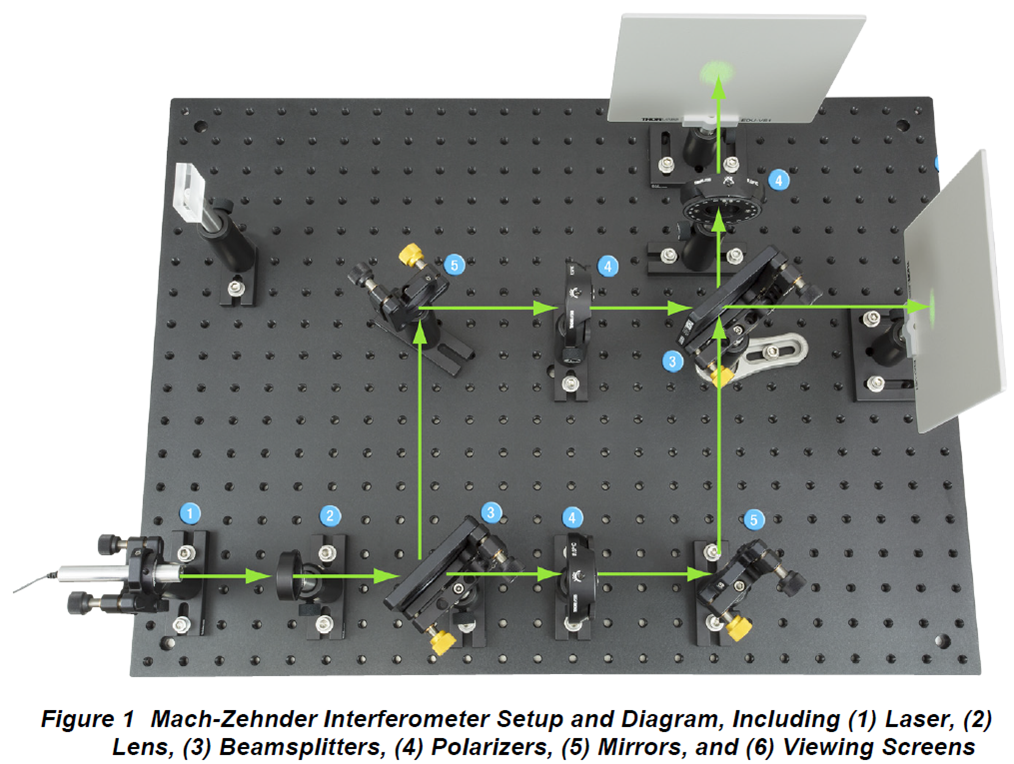
\includegraphics[width=0.9\textwidth]{4Montage.png}
		\label{pic:4Montage}
	\end{figure}
	
	\begin{figure}[h!]
		\caption{ Пример компоновки на монтажной плите проектора для лазерного шоу компании Arctos }
		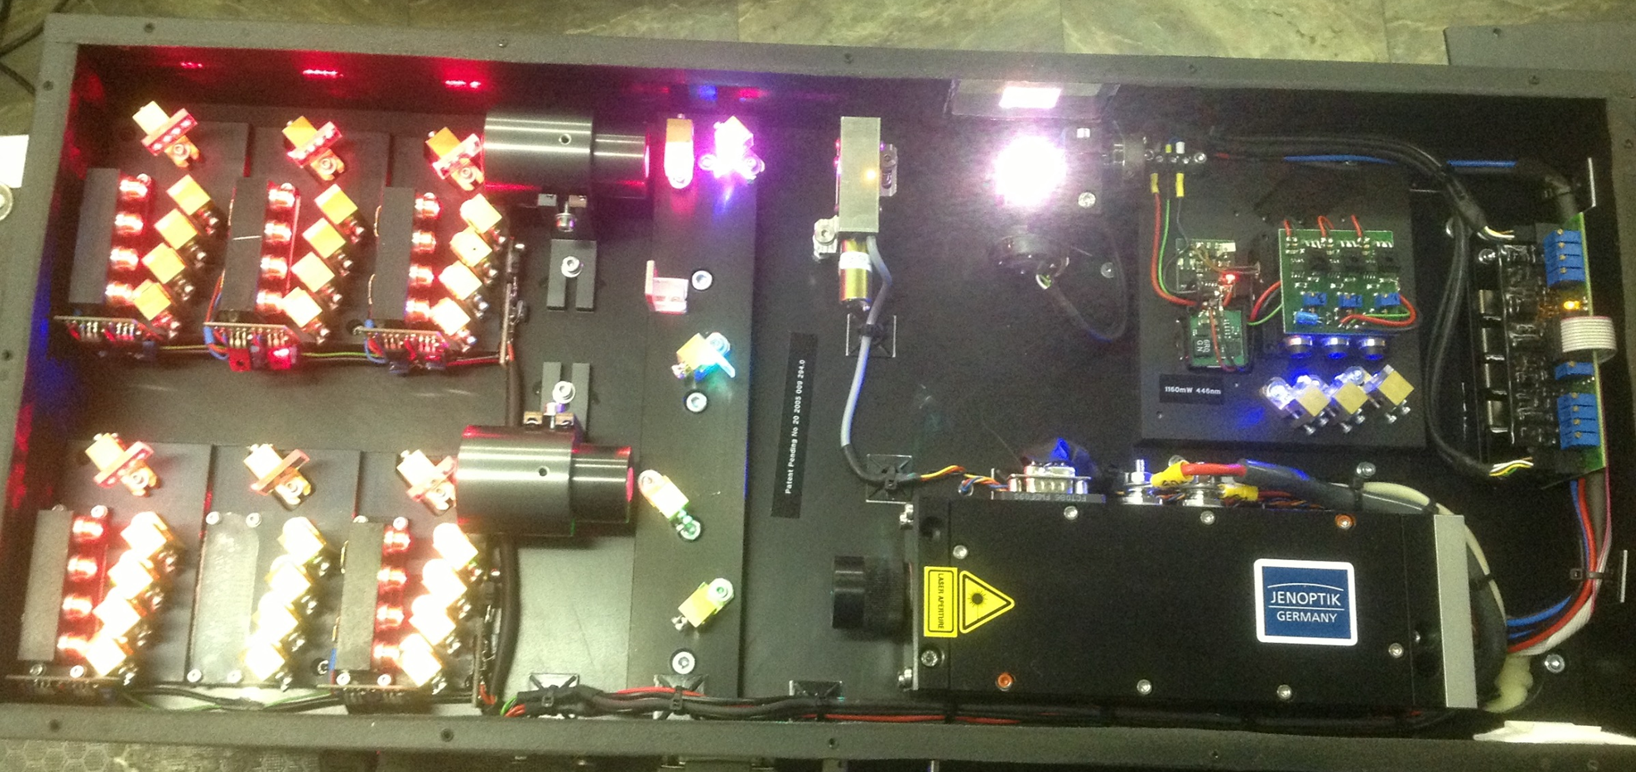
\includegraphics[width=0.9\textwidth]{4LaserShow.png}
		\label{pic:4LaserShow}
	\end{figure}
	
	\item На монтажных платах с колонками. Способ компоновки на монтажных платах с колонками является развитием предыдущего способа при расположении элементов оптической схемы в разных плоскостях. Как видно на рис.~\ref{pic:4plata}, в конструкцию прибора включены три монтажные платы~1, соединенные между собой колонками~2. На двух верхних платах в оправах, на стойках и кронштейнах размещены оптические элементы, а на нижней плате закреплен блок усилителей.
	
	\begin{figure}[h!]
		\caption{Компоновка на монтажных платах с колонками}
		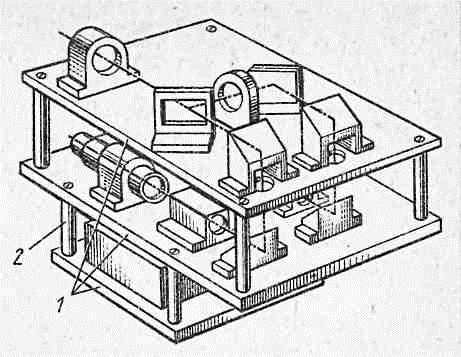
\includegraphics[width=0.9\textwidth]{4plata.png}
		\label{pic:4plata}
	\end{figure}
	
	\item С нанизыванием узлов. Компоновку с нанизыванием узлов применяют, если узлы прибора собраны на платах, имеющих одинаковую конфигурацию. Так, узлы объектива 1, светоделителя 2, модулятора 3, конденсоров 4, приемников излучения 5 и электронный блок 6 фазового угломера (рис.~\ref{pic:4uzel}~и \ref{pic:4uzel}) смонтированы на пластинах круглой формы, нанизанных на систему из трех стержней~7.
	
	\begin{figure}[h!]
		\caption{Компоновка с нанизыванием узлов}
		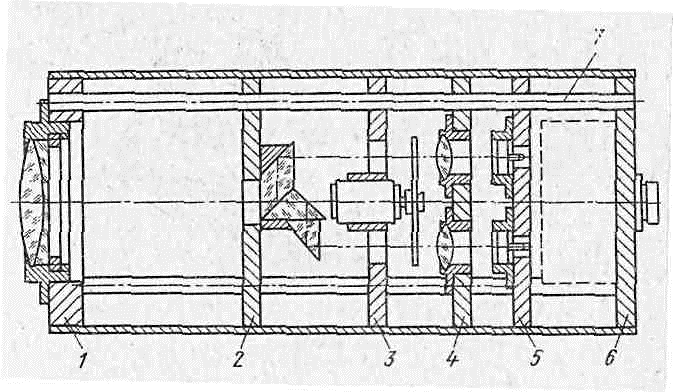
\includegraphics[width=1\textwidth]{4uzel.png}
		\label{pic:4uzel}
	\end{figure}
	
	\begin{figure}[h!]
		\caption{Компоновка с нанизыванием узлов компании Thorlabs}
		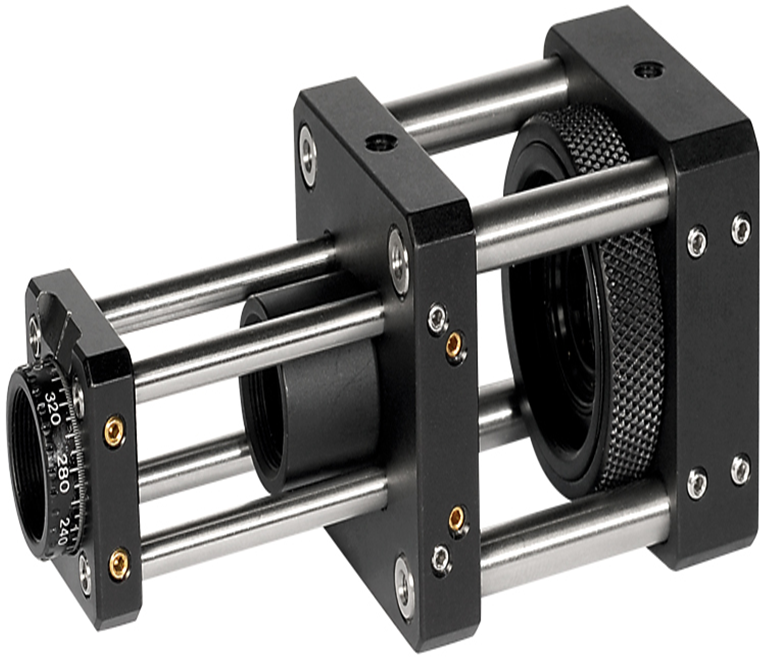
\includegraphics[width=0.7\textwidth]{4Nanizivanie.png}
		\label{pic:4Nanizivanie}
	\end{figure}
	
	Достоинством этой схемы компоновки являются единообразие несущих элементов, простота сборки и юстировки. Жесткость и стабильность такой конструкции не намного ниже аналогичных параметров конструкции при компоновке с применением трубы в качестве несущего элемента, а масса прибора значительно меньше. Поэтому компоновку с нанизыванием узлов часто применяют при конструировании крупногабаритных приборов, которые имеют осесимметричную схему и к которым предъявляют повышенные требования относительно жесткости.
	
	\item С использованием направляющей. Компоновка с использованием направляющей применяется при проектировании приборов, в которых при эксплуатации требуется изменять взаимное положение элементов (изменять расстояние между элементами, менять их местами) В основном это относится к стендовому оборудованию или приборам для научных исследований. В качестве примера такой компоновки можно привести оптическую скамью ОСК-2. Подобного рода компоновку выполняют также на направляющей треугольного профиля.Направляющая типа <<Ласточкин хвост>> показана на рис.~\ref{pic:4Lastochkin}.
	
	\begin{figure}[h!]
		\caption{Компоновка на монтажных платах с колонками}
		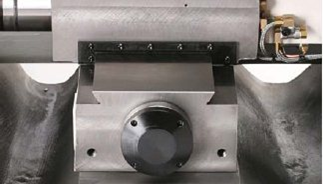
\includegraphics[width=0.5\textwidth]{4Lastochkin.png}
		\label{pic:4Lastochkin}
	\end{figure}
	
	\item В стойку с использованием модульных узлов и блоков. Компоновку на базе модульных узлов и блоков применяют в основном при конструировании электронных стоек.
	
	\item В кожух в виде пульта.
\end{enumerate}

Способы компоновки 3-8 в большинстве случаев требуют применения кожуха, защищающего прибор от посторонних засветок и воздействия окружающей среды. Во многих случаях при конструировании оптических блоков ОЭП используют одновременно несколько рассмотренных способов компоновки

\begin{flushleft}
	\textbf{Некоторые примеры компоновки}
\end{flushleft}

Так как ОЭП содержат функциональные устройства с различными физическими принципами действия (оптические, механические, электронные), которые должны располагаться в едином корпусе и быть защищены от внешних воздействий (посторонних засветок, механического контакта, загрязнений, влаги), то часто несущим элементом является коробчатый корпус, получаемый литьем из металлических или пластмассовых материалов.

Командно-регистрационные устройства ОЭП выполняются, как правило, в виде автономных блоков по принципу блочно-модульной конструкции. На рис.~\ref{pic:4block} изображен подобный автономный блок с несущим элементом -- стойкой, в которую вдвигаются функциональные блоки (модули) 1-7. На рис.~\ref{pic:4NI} показана компоновка модульной PXI-платформы компании National Instruments.

\begin{figure}[H]
	\caption{Компоновка командно-регистрационного устройства}
	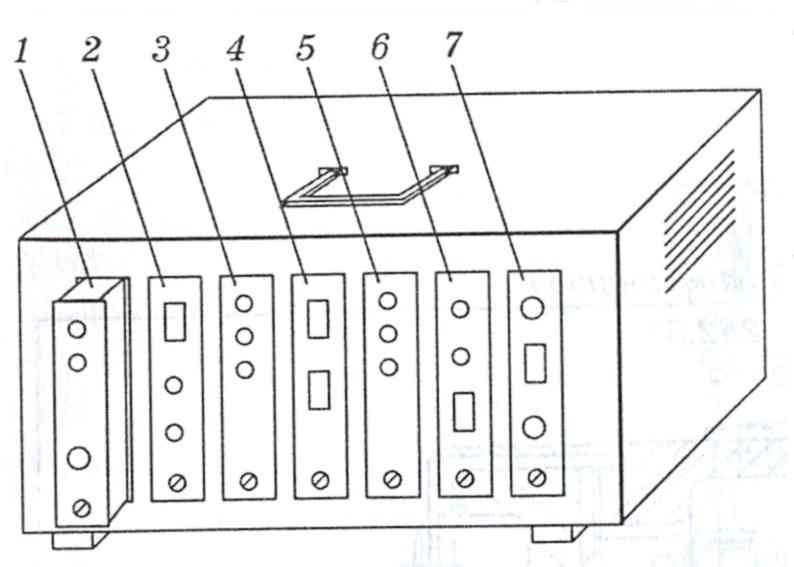
\includegraphics[width=0.6\textwidth]{4block.png}
	\label{pic:4block}
\end{figure}

\begin{figure}[H]
	\caption{ Компоновка модульной PXI-платформы компании National Instruments }
	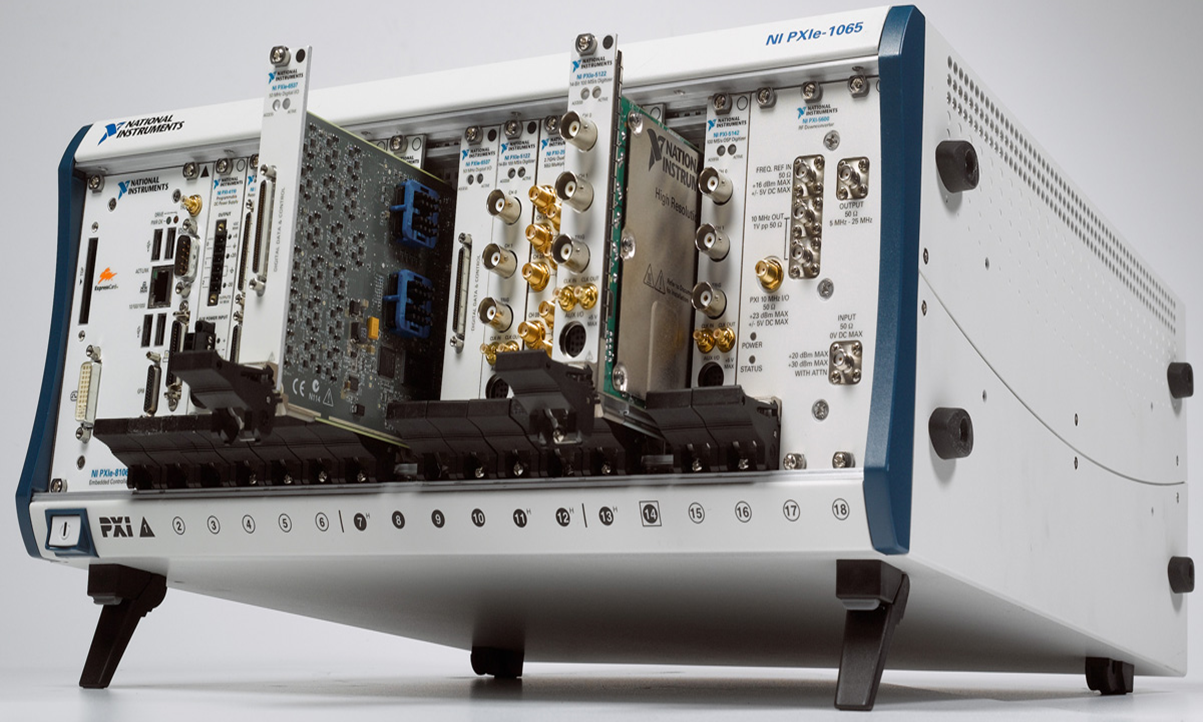
\includegraphics[width=0.8\textwidth]{4NI.png}
	\label{pic:4NI}
\end{figure}

Компонуя оптическую схему прибора, часто используют зеркально-призменные системы (ЗПС). При этом целесообразно учитывать свойства этих систем, позволяющие упростить юстировку при сборке и выполнить конструкцию более устойчивой к разъюстировкам в процессе эксплуатации.

На рис.~\ref{pic:4prism}, а показана схема компоновки объектива~1 и фотоприемника~3 с помощью прямоугольной призмы~2. Для центрировки и фокусировки изображения на фотоприемник призму юстируют. Если сместить ее по оси $ Z $ (или в другом произвольном направлении), то появляется смещение изображения по приемнику вдоль оси $ X' $ и вдоль оси $ Z' $, т.е. юстировка является зависимой. Кроме этого, при такой подвижке возможны повороты призмы вокруг оси $ Y $, которые вызовут смещение и наклон изображения.

Компоновка конструкции с помощью пентапризмы (рис.~\ref{pic:4prism}~б) более предпочтительна, так как, сдвигая ее вдоль оси $ X $, добиваются центрировки изображения (его смещения вдоль оси $ X' $), а сдвигом вдоль оси $ Z $ -- юстировка будет менее трудоемкой, так как является независимой.

\begin{figure}[h!]
	\caption{Компоновки конструкции призмами}
	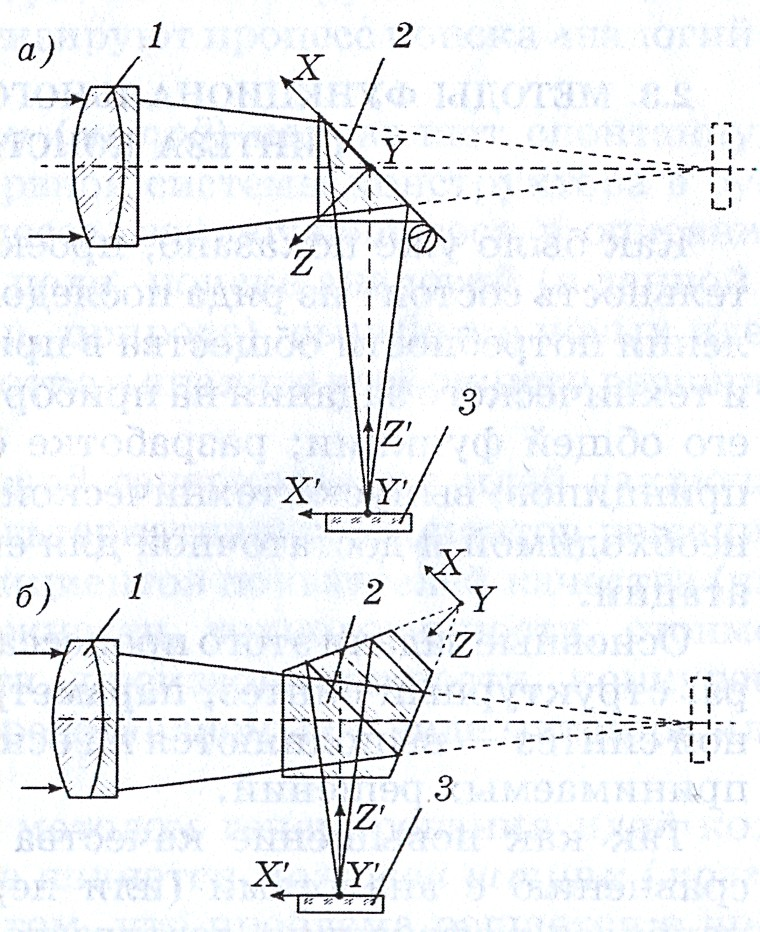
\includegraphics[width=0.7\textwidth]{4prism.png}
	\label{pic:4prism}
\end{figure}

Еще один пример компоновки с использованием принципа инверсии (Под конструктивной инверсией понимают перестановку, обращение или перераспределение роли и функций деталей, узлов, их элементов для улучшения свойств конструкции без изменения ее общей целевой функции) для упрощения конструкции корпуса телеобъектива показан на рис.~\ref{pic:4inversion}. В первоначальном варианте (рис.~\ref{pic:4inversion}~а) изменение воздушного промежутка $ d $ между подвижным положительным~2 и неподвижным отрицательным~3 компонентами телеобъектива достигалось вращением оправы положительного компонента, сопрягаемого с корпусом по резьбе. Так как диаметр оправы компонента~2 и диаметр компонента~3 существенно различаются, конструкция корпуса~1 получилась сложной и нетехнологичной.

Второй вариант конструкции телеобъектива (рис.~\ref{pic:4inversion}~б), где перемещается по резьбе оправа~4 отрицательного компонента (относительно неподвижного положительного), позволяет упростить конструкцию корпуса~5, создает возможность изготовить его из стандартной трубы, сократить расход материала.

\begin{figure}[h!]
	\caption{Конструктивная инверсия элементов объектива}
	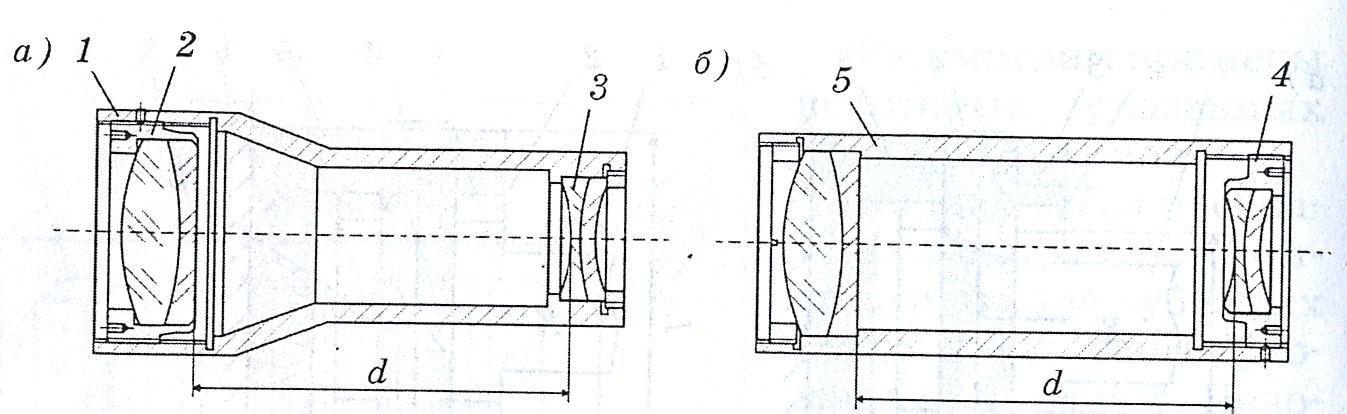
\includegraphics[width=1\textwidth]{4inversion.png}
	\label{pic:4inversion}
\end{figure}

\chapter{Линзы и способы их крепления}
\section{Линзы и линзовые блоки (склейки)}

\textit{Линзами} называются оптические детали из однородных, прозрачных для оптического диапазона длин волн материалов, ограниченные двумя преломляющими рабочими поверхностями, из которых по крайней мере одна является поверхностью тела вращения (сферическая, асферическая, цилиндрическая, коническая поверхности), применяемые в оптических приборах для преобразования формы пучков излучения и построения изображений различных объектов.

По характеру преобразования пучка различают собирающие и рассеивающие линзы; по сочетанию форм рабочих преломляющих поверхностей их подразделяют на плосковыпуклые (вогнутые) (рис.~\ref{pic:5lenses}~а,~г), двояковыпуклые (вогнутые) (рис.~\ref{pic:5lenses}~б,~д), мениски (с радиусами кривизны, одинаковыми по знаку) (рис.~\ref{pic:5lenses}~в), бифокальные (с разными радиусами кривизны на частях одной из рабочих поверхностей) (рис.~\ref{pic:5lenses}~е), линзы Френеля (с плоской и ступенчатой поверхностями) (рис.~\ref{pic:5lenses}~ж), аксиконы (с плоской и конической поверхностями) (рис.~\ref{pic:5lenses}~з).

\begin{figure}[h!]
	\caption{Линзы}
	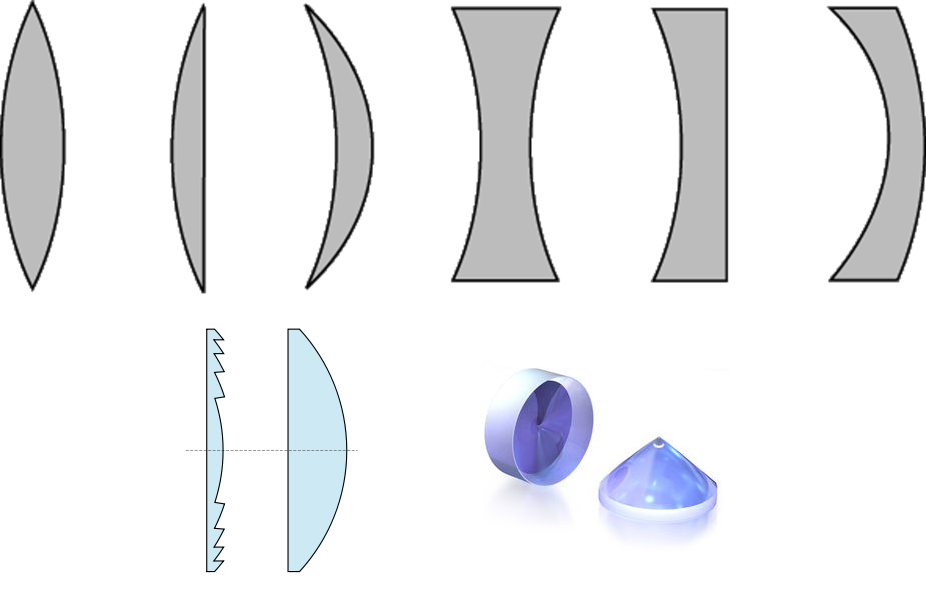
\includegraphics[width=1\textwidth]{5lenses.png}
	\label{pic:5lenses}
\end{figure}

Форма боковой поверхности линзы чаще всего выполняется круглой (цилиндрической), что является наиболее технологичным при изготовлении и закреплении в оправе (иногда форма боковой поверхности выполняется прямоугольной или сегментарной).

\textbf{Конструктивные параметры} линз подразделяют на \textit{расчетные} и \textit{конструкторские}.

К \textit{расчетным параметрам} (рис.~\ref{pic:5draw},~\ref{pic:5faska}) относят оптические характеристики и показатели качества материала линзы, ее световые диаметры на рабочих поверхностях (диаметр поверхности линзы, пропускающей световой поток), толщину линзы по оптической оси, радиусы кривизны (или параметры формы) преломляющих поверхностей, фокусное расстояние и вершинные фокальные отрезки, допустимые значения погрешностей изготовления оптических поверхностей (погрешности формы, децентрировку\footnote{Децентрировка -- несовпадение оптической оси линзы с геометрической осью}, отклонение толщины по оси), вид оптических покрытий. Эти данные определяются при габаритном, аберрационном, светотехническом расчетах оптической системы.

К \textit{конструкторским параметрам} (рис.~\ref{pic:5draw}--\ref{pic:5lensdraw}), относят полный диаметр линзы (или ее размеры, при некруглой форме), параметры фасок, толщину по краю, габаритный размер вдоль оси, чистоту рабочих и шероховатость нерабочих поверхностей, вид покрытия нерабочих (матовых) поверхностей, допуски на погрешности не справочных параметров. Эти параметры определяют в процессе конструирования при окончательном оформлении ее конструкции.

\begin{figure}[h!]
	\caption{Чертеж линзы без защитных фасок}
	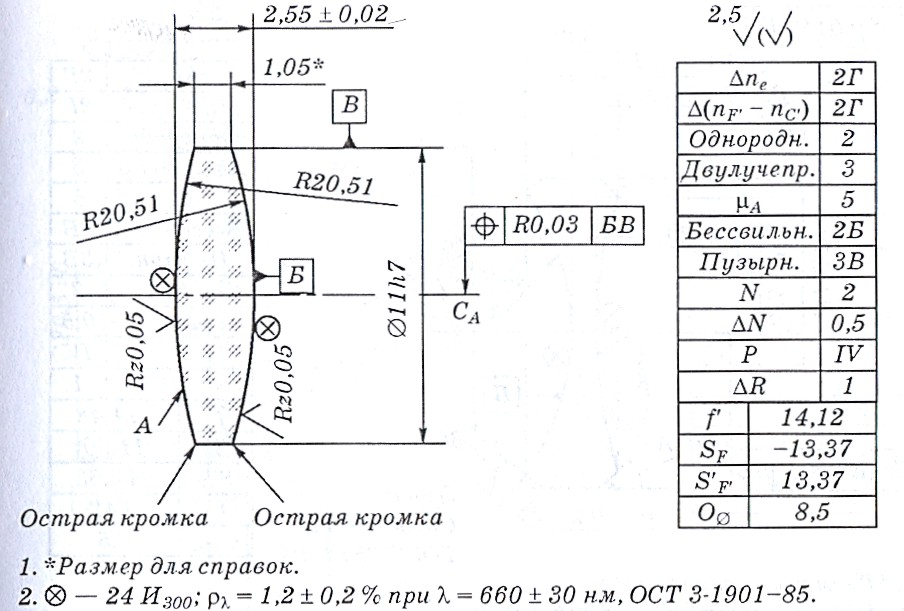
\includegraphics[width=1\textwidth]{5draw.png}
	\label{pic:5draw}
\end{figure}

\begin{figure}[h!]
	\caption{Линза с конструктивной фаской}
	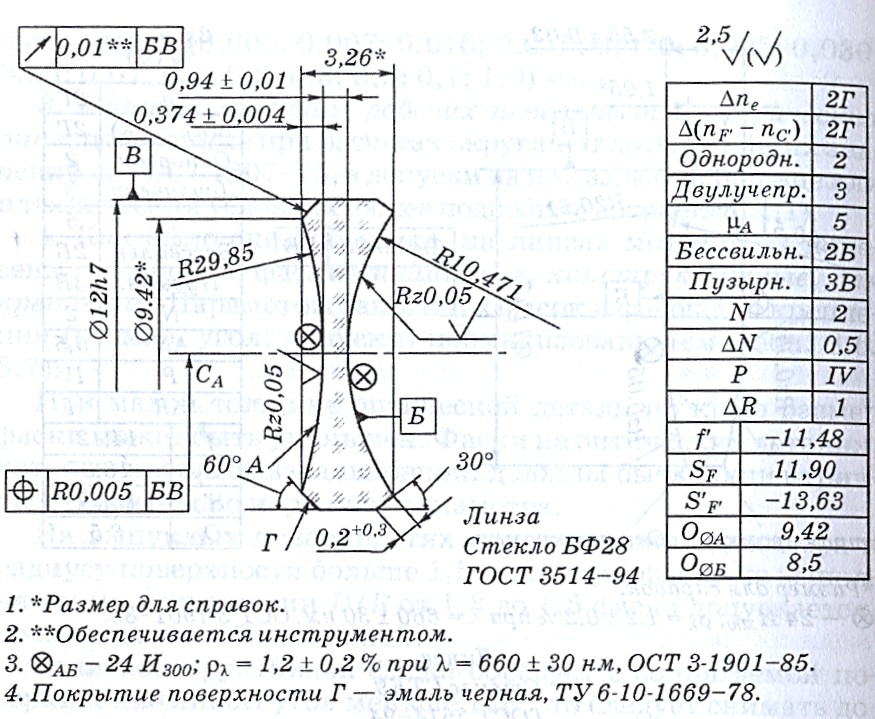
\includegraphics[width=1\textwidth]{5faska.png}
	\label{pic:5faska}
\end{figure}

Рассмотрим некоторые аспекты определения конструктивных параметров.
\begin{enumerate}
	
\item Для закрепления линзы в оправе ее полный диаметр выполняют несколько больше светового. Минимальное значение полного диаметра линзы зависит от светового диаметра и способа закрепления. Окончательный размер полного диаметра округляется до ближайшего (большего) нормального диаметра по действующим стандартам. Поля допусков на полный диаметр линзы должны образовывать в соединении с оправой линзы посадку с зазором, поэтому в зависимости от необходимого значения гарантированного зазора и точности центрирования обычно проставляют следующие допуски на диаметры линз:

$ g6, f7 $ -- высокая точность (технический уровень точности);
$ h8, f9, e9 $ -- средняя точность (производственный уровень точности);
$ d9, c11, d11 $ -- пониженная точность (экономический уровень точности).

Заметим, что в соединении линзы с оправой должен быть обеспечен необходимый <<температурный>> зазор, а также то, что точность центрировки линзы в оправе зависит не только от допуска на ее диаметр, но и от выполнения условия самоцентрирования и использования результативной обработки оправы после закрепления линзы.

\item Исходя из требований технологии при конструировании положительных линз необходимо обеспечивать минимальную толщину по их краю в соответствии с рекомендациями, приведенными в соответствующих справочных материалах, а толщина по оси отрицательных линз в зависимости от ее диаметра и необходимой точности формы рабочих поверхностей должна соответствовать рекомендациям действующих стандартов (в пределах от $ 0,05D $ до $ 0,09D  $ в зависимости от диаметра линзы).

Рассчитанные предельные допуски на толщину линз вдоль оси (исходя из их влияния на качество изображения) округляют до ближайшего меньшего значения из ряда значений, приведенного в действующих стандартах [$ \pm(0,005; 0,007; 0,010; 0,015; 0,020; 0,025; 0,030-0,05; 0,07; 0,1; 0,2; 0,3; 0,5; 0,7; 1,0) $ мм].

\item Радиусы кривизны рабочих поверхностей сферических линз, полученные при расчетах, округляют до ближайших значений по действующим стандартам, а допуски на них задают в таблице или в технических условиях.

\item На линзах могут быть нанесены следующие фаски (рис.~\ref{pic:5faska}): защитные, конструктивные, для крепления. Параметры защитных фасок и фасок для крепления (размер, угол, допуски) нормализованы (приведены в соответствующих таблицах).

При малой толщине оптической детали по краю размер фаски может быть уменьшен. Фаски на оптических деталях, которые крепятся завальцовкой, должны быть концентричны относительно наружного диаметра.

На выпуклых поверхностях при отношении диаметра к радиусу поверхности больше 1,5 защитную фаску не выполняют; при отношении $ D/R $ от 1,3 до 1,5 фаска допускается, но не является обязательной.

На некоторых линзах, собранных в линзовую систему групповым способом <<насыпным без промежуточных колец>>, защитные фаски на кромках не снимают. Обусловлено это тем, что при применении данного способа крепления линзы в системе устанавливаются друг по другу рабочими поверхностями и кромками (фасками), поэтому значительные погрешности защитных фасок вызывают погрешности воздушных промежутков между компонентами и нарушают центрировку линз в системе (рис.~\ref{pic:5draw}).

Для точной центрировки линзы и обеспечения номинального расстояния между компонентами на соответствующей кромке линзы выполняется конструктивная фаска, которая может быть нанесена не вручную, а при помощи инструмента с последующим контролем ее размера (расположения) и биения (рис.~\ref{pic:5faska}).

\item В качестве материала для линз используется в основном оптическое стекло различных марок. Однако в последнее десятилетие широкое применение получили линзы из оптических полимеров (полиметилметакрилат, полистирол, поликарбонат, сополимер, zeonex), в частности в массовом производстве линз фотографической техники широкого потребления, линз осветительных систем (например, линз Френеля), очковых линз, линз окуляров, лупы, что существенно облегчает их массу и уменьшает стоимость.

Линзы, работающие в инфракрасной и ультрафиолетовой областях спектра, изготавливаются из специальных марок стекол (К515, ИКС), кварцевого стекла (КУ-1), оптической керамики, оптических кристаллов (флюорита, сильвина, фтористого лития, германия).

\item Оптические характеристики линзы: $ f, f' $ -- фокусные расстояния (переднее и заднее); $ S_F, S'_{F'} $  -- передний и задний фокальные отрезки; и расчетные световые диаметры на рабочих поверхностях линз указывают в третьей части таблицы, причем один из фокальных отрезков при необходимости может указываться с допуском.

\item Допуск на децентрировку рабочей поверхности линзы выражают в долях миллиметра и проставляют в поле чертежа, в специальной рамке, содержащем три поля, в первом указывают значок вида допуска децентрировки (позиционный, перпендикулярности или биения плоской поверхности, формы заданной поверхности), во втором -- численное значение допуска, в третьем указывают базы, относительно которых следует контролировать децентрировку (рис.~\ref{pic:5draw}, \ref{pic:5faska}).

При контроле децентрировки круглую линзу (или линзовый блок) устанавливают одной из базовых поверхностей на кольцевую опору, поджимают другой базовой поверхностью к ножевидному упору и приводят во вращение. Измеренное при этом биение центра кривизны рабочей поверхности (или биение плоской поверхности) относительно базовой оси (создаваемой базовыми поверхностями) является мерой децентрировки. Контроль децентрировки некруглых сферических линз, цилиндрических и асферических линз производится с помощью специальных методов и приборов.

Высокий уровень точности центрировки линз соответствует значениям их децентрировки в диапазоне 0,002-0,005 мм, среднему уровню соответствует диапазон 0,005-0,01 мм и пониженному уровню -- 0,01-0,02 мм.

\item На рабочие  поверхности  линзы  могут  быть нанесены различные виды оптических покрытий (просветляющих, зеркальных, светоделительных и поглощающих), а для уменьшения бликов и защиты детали от влияния внешней среды выполняют покрытия их боковых поверхностей и фасок.
\end{enumerate}

\begin{figure}[h!]
	\caption{Чертеж линзы без защитных фасок}
	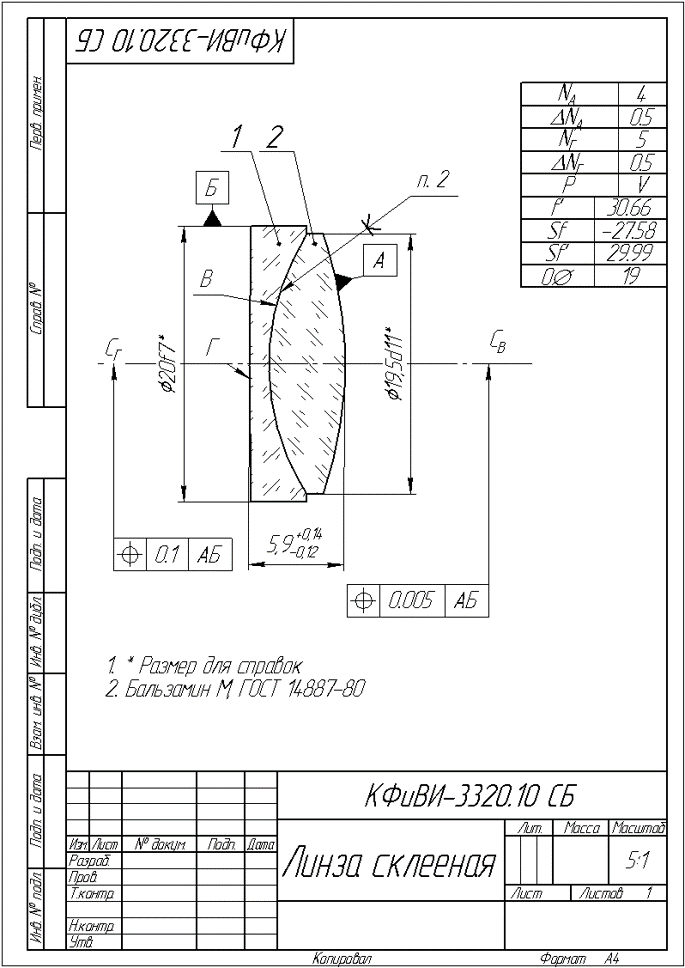
\includegraphics[width=0.7\textwidth]{5lensdraw.png}
	\label{pic:5lensdraw}
\end{figure}

Одиночные сферические линзы вследствие больших аберраций редко применяются как самостоятельные элементы оптических приборов. Чаще используются комбинации из нескольких линз, склеенные линзы (склейки, линзовые блоки), выполняющие те же функции, что и одиночные линзы, но со значительно меньшими аберрациями.

Большое распространение в ОЭП получили склеенные блоки из двух линз (реже трех линз и более) -- положительной и отрицательной, изготовленные из стекол различных марок типа крон и флинт (рис.~\ref{pic:5skleyka}). Они применяются, например, в качестве объективов и оборачивающих линз телескопических приборов. У двухлинзовых склеек могут быть хорошо исправлены сферическая аберрация, хроматизм и кома, другие же аберрации устранить достаточно полно невозможно.

\begin{figure}[h!]
	\caption{Склейки линз}
	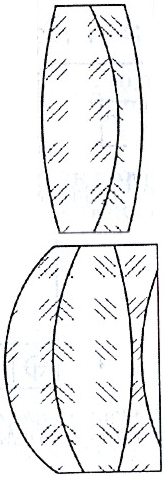
\includegraphics[width=0.5\textwidth]{5skleyka.png}
	\label{pic:5skleyka}
\end{figure}

Для склеивания линз (и других оптических деталей) применяют специальные оптические клеи: пихтовый бальзам, бальзамин, бальзамин-М, акриловый, УФ-215М, эпоксидный и другие оптические клеи, которые обладают рядом необходимых свойств и характеристик (высокая прозрачность в спектральном диапазоне, близость показателя преломления к показателям преломлений склеиваемых материалов, оптическая однородность, отсутствие возникновения существенных напряжений при полимеризации, стабильность свойств во времени, тепло- и морозостойкость).

Основные марки оптических клеев и их свойства приведены в действующих стандартах, рекомендации по использованию тех или иных марок клеев при склеивании линз и других оптических деталей в зависимости от условий их работы приведены в соответствующих справочниках.

Чертеж линзового блока оформляется в соответствии с требованиями, приведенными ранее. На чертеже блока, являющегося сборочной единицей, указываются только те параметры, которые должны быть выполнены и проконтролированы в процессе сборки (склейки): центрировка и толщина склеенного блока, отсутствие деформаций наружных рабочих поверхностей, их чистота. Поэтому верхняя часть таблицы -- требования к материалу -- на чертеже склеенного блока линз отсутствует, таблица состоит только из двух частей: требований к сборке и оптических характеристик.

В склейке одна из линз является базовой, а другая -- присоединяемой (приклеиваемой). При конструировании деталей, входящих в склейку, как правило, на полный диаметр базовой линзы назначается допуск $ e9 $, для приклеиваемой -- $ d10 $ или $ d11 $. Допускается выполнять приклеиваемую линзу с уменьшенным диаметром по номиналу по сравнению с базовой линзой на 0,2 -- 0,4~мм на диаметр.

При определении базовой и приклеиваемой линз следует учитывать следующее:
\begin{itemize}
\item в качестве базовой следует выбирать линзу с большей толщиной по краю для удобства базирования при склеивании и контроле готового узла;
\item в качестве базовой следует выбрать ту деталь, у которой в склейку идет вогнутая поверхность, поскольку клей при склеивании не должен вытекать из соединительного шва, а напротив, должен заполнять все образующиеся пустоты при сопряжении двух линз;
\item наружный радиус базовой линзы желательно иметь большего значения, чем наружный радиус приклеиваемой линзы для более точного и удобного изготовления склейки;
\item желательно, чтобы показатель преломления материала базовой линзы не значительно отличался от показателя преломления клея по сравнению с разницей показателей преломления клея и материала приклеиваемой линзы;
\item необходимо, чтобы радиус базовой поверхности был больше радиуса приклеиваемой поверхности (это касается как базовой, так и приклеиваемой линз);
\item желательно, чтобы базовая поверхность базовой линзы оставалась базовой поверхностью и для всей склейки;
\item желательно, чтобы у приклеиваемой линзы базовой являлась та поверхность, которая уходит в склейку.
\end{itemize}

Допуск на децентрировку базовой линзы ставится более жесткий, чем допуск на приклеиваемую линзу. Особенно это касается случая, когда показатель преломления материала приклеиваемой линзы фактически совпадает с показателем преломления клея.

Допуск на суммарную толщину склейки линз рассчитывается следующим образом: \\ $ \Delta d_\text{скл} = \Delta d_\text{баз} + \Delta d_\text{прик} + 0,01$ , например:
\[ d_\text{баз} = 1 \pm 0,01; \]  
\[ d_\text{пр} = 4 \pm 0,02; \] 
\[ d_\text{скл} = 1_{-0,01}^{+0,01}  + 4_{-0,01}^{+0,01} + 0,01 = 5. \]

На наружные рабочие поверхности склейки линз могут быть нанесены оптические покрытия, а боковые поверхности и фаски (матовые поверхности) покрывают защитными эмалями.

\section{Общие требования к оптическим узлам и устройствам}
Сборочные единицы, выполняющие в приборе определенные функции только совместно с другими составными частями, но объединенные в процессе проектирования и изготовления (сборки) в единую систему, называются конструктивными узлами. Они обычно состоят из относительно небольшого количества сопряженных друг с другом деталей, среди которых выделяют рабочую, базовую (оправу, корпус) и вспомогательные (крепежные, ориентирующие, технологические). 

Типичными представителями конструктивных узлов оптических приборов являются узлы крепления оптических деталей и узлы фотоприемников. Прежде чем рассмотреть типовые конструкции таких узлов, перечислим некоторые общие требования к ним и состоящим из них функциональным устройствам.

\begin{enumerate}
	
\item Конструкция узла должна обеспечить точное расположение рабочей детали (ее рабочих элементов) относительно базовой детали (базового элемента оправы).

\item Крепление должно быть надежным; не допускается изменение положения рабочей детали относительно оправы после закрепления в процессе эксплуатации.

\item В конструкции не должно возникать опасных (объемных) деформаций рабочей и базовой деталей и внутренних напряжений в них при закреплении и в процессе эксплуатации.

При силовом замыкании крепежные элементы не должны вызывать деформации изгиба или кручения. Допускается деформация сжатия (контактная). Для уменьшения деформаций из-за погрешностей размеров, формы и положения элементов деталей между крепежной деталью и оптической следует устанавливать упругие или эластичные прокладки (металлические пружинные кольца, прокладки из пробки, картона, поранита).

Обязательно должно быть обеспечено отсутствие температурных деформаций (или смещений рабочей детали относительно базовой) при перепадах температуры.
\item Конструкция узла при необходимости должна обеспечивать возможность юстировки рабочей детали. Потребность в юстировке может быть нужна в двух случаях: для точного расположения рабочей детали относительно оправы (например, центрирование линзы при ее сборке относительно базовой оси оправы); для обеспечения требуемого расположения рабочей детали относительно рабочих деталей или баз других узлов (например, фокусировка линзы на фотоприемник). Поэтому для первого случая конструкция узла должна обеспечивать юстировочные подвижки рабочей детали относительно оправы в процессе ее закрепления, для второго~-- подвижки рабочей детали в оправе или вместе с ней (т.е.~всего узла) относительно других узлов в процессе либо после сборки функционального устройства или всего прибора.

\item Конструкция узла должна быть технологичной в отношении изготовления деталей и особенно в отношении их сборки (свободный доступ инструмента, возможность автоматизации сборки, удобство контроля, доступность и простота обслуживания и замены малонадежных элементов).

\item Габаритные размеры узла желательно минимизировать, чтобы обеспечить отсутствие срезания пучка лучей, появление бликов и рассеянного света в системе.

\item Конструкции функциональных устройств должны быть унифицированы по принципам построения, целевым характеристикам, присоединительным размерам, номиналам электропитания.

\item Фактически ни одно функциональное устройство не обходится без юстировки его показателей качества, поэтому надо знать необходимые юстировочные операции типовых функциональных устройств, методику их выполнения (с перечнем необходимого контрольного оборудования), уметь рассчитывать требования к юстировке и заложить в конструкции устройств возможность ее осуществления.

\end{enumerate}

Выполнение перечисленных требований основывается на использовании принципов и правил конструирования соединений, узлов и функциональных устройств.

%\section{Конструкции узлов крепления круглых оптических\\ деталей и линзовых систем}

К основным способам крепления линз и других круглых оптических деталей относятся: крепление завальцовкой, крепление приклеиванием, крепление резьбовым кольцом. При необходимости, когда приходится учитывать особые условия и требования, связанные с габаритными размерами, назначением, условиями эксплуатации оптических деталей, могут использоваться вспомогательные способы крепления: проволочным кольцом, прижимными планками, накладным кольцом, специальными элементами или специальной конструкцией оправы. Указанные названия способов крепления определены видом замыкания рабочей (оптической) детали с базовой (оправой) в соединении или видом крепежной детали.

\begin{flushleft}
	\textbf{Крепление завальцовкой}
\end{flushleft}

При этом способе крепления линза поджимается к опорному уступу тонким буртиком, выполненным на оправе. Операция завальцовки производится на токарном или сверлильном станках при помощи роликов, специальных инструментов или ультразвуком. В результате тонкий буртик оправы (рис.~\ref{pic:5zavalcovka}) деформируется и загибается по всей окружности на специально выполненную фаску линзы.

\begin{figure}[h!]
%	\caption{Крепление линзы завальцовкой:\\ а -- размеры, буртика; б -- общий вид}
	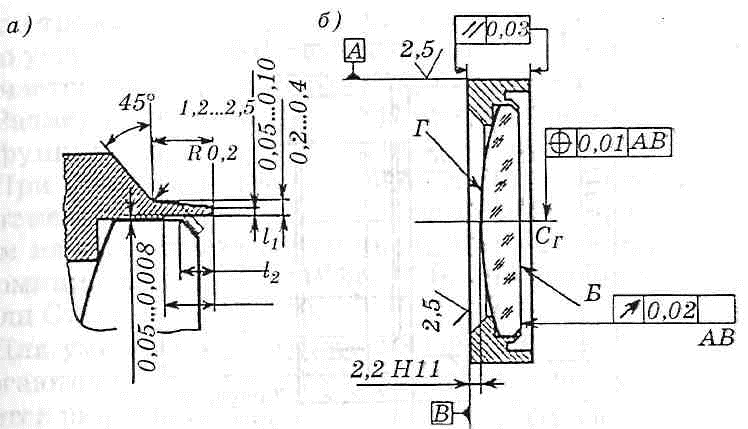
\includegraphics[width=1\textwidth]{5zavalcovka.png}
	\label{pic:5zavalcovka}
\end{figure}

Чтобы не образовалось сколов кромки линзы при загибании буртика, на внутренней поверхности оправы выполняют выборку $ l_2 $. Размеры элементов загибаемого буртика берутся из справочника конструктора оптико-механических приборов. 

Преимуществами этого метода крепления являются простота и компактность конструкции соединения. Закрепляющий тонкий буртик, обладая упругими свойствами, обеспечивает силовое замыкание линзы без напряжений, а также компенсирует температурные деформации. Возможна автоматизация сборки соединения. Кроме того, в процессе завальцовки линзы можно выполнять ее частичную центрировку.

Недостатки: конструкция неразборная; существует ограничение на массу закрепляемой линзы (склеенного блока). Ограничение объясняется тем, что тонкий (до 0,1 мм) загибаемый буртик не обеспечивает надежного крепления массивных линз. Выполнение буртика большей толщины исключает его упругие свойства и может привести к выколкам кромки линзы в процессе завальцовки и ухудшить эксплуатационные свойства соединения. Поэтому крепление завальцовкой рекомендуется применять для линз от 6 до 80 мм, а склеенных блоков -- до 50 мм.

Технология завальцовки предполагает наличие специальных оборудования, приспособлений и определенной квалификации сборщика. Точность центрирования линзы в оправе может быть несколько ниже, чем при других способах крепления из-за того, что закрепляющий буртик ложится на матовую поверхность нецентрированной фаски линзы.

При креплении завальцовкой для оправ обычно используют легко деформируемые, но упругие материалы. Наилучшим из них является латунь ЛС59-1. Также применяются алюминиевые сплавы Д1, Д6, Д16, В95 и низкоуглеродистые стали Сталь 20, Сталь 30.

Для уменьшения отражения света от стенок оправы подвергаются чернению, а на внутренних поверхностях выполняется рифление.

Завальцовка иногда используется при креплении несклеенных блоков (состоящих из двух-трех) линз и весьма часто -- при креплении сеток, светофильтров, защитных стекол и других деталей, имеющих круглую форму.

\begin{flushleft}
	\textbf{Крепление приклеиванием}
\end{flushleft}

В настоящее время способ крепления линз и других круглых оптических деталей приклеиванием к оправам является все более и более используемым. Причиной этому служит появление новых клеящих веществ с оптимальными свойствами для соединения оптических деталей с оправами (обеспечение надежности соединения, эластичность, отсутствие деформаций в слоях клея, хорошая адгезия к различным материалам, способность сохранять свойства при внешних воздействиях, стабильность во времени).

В результате данные узлы крепления имеют ряд положительных качеств:
\begin{itemize}
\item конструктивная простота узла крепления, а также снижение его массы и габаритных размеров;
\item возможность закрепления линз, крепление которых традиционными способами затруднено, например линз малого диаметра (до 6~мм), с крутыми радиусами кривизны и тонкими краями (рис.~\ref{pic:5glue}), при некруглой форме базовых поверхностей;
\item отсутствие деформаций и напряжений в оптической детали при внешних воздействиях на узел крепления (например, при изменении температуры) благодаря упругим свойствам клеящих веществ;
\item возможность корректировки положения оптической детали до момента затвердевания клеящего вещества;
\item обеспечение герметизации соединения;
\item относительная простота автоматизации процесса сборки.
\end{itemize}

\begin{figure}[h!]
	\caption{Крепление линз объектива приклеиванием}
	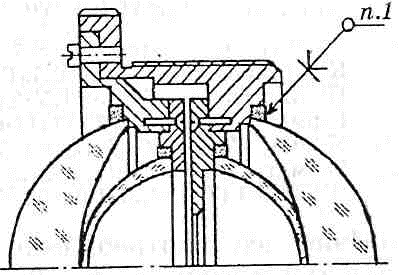
\includegraphics[width=0.6\textwidth]{5glue.png}
	\label{pic:5glue}
\end{figure}

Заметим, что этот способ наиболее часто применяется также для крепления линз приклеиванием в случаях, когда они имеют некруглую форму боковых поверхностей.

Качество соединения линзы с оправой зависит от согласованности материалов, входящих в узел крепления компонентов. Для этого необходимо знать физико-механические свойства клеящего вещества, линзы и оправы.

Материал, из которого изготовлены линзы для последующего крепления приклеиванием, может быть любым. Чистота обработки поверхности стекла в месте крепления не оказывает существенного влияния на скрепляющее свойство. Поэтому приклеиваемая поверхность линзы может быть шлифованной.

Оправы, к которым приклеиваются линзы, изготавливают из алюминиевых сплавов, латуни, стали, титана и его сплавов: ВТ1-0, ОТ4, ВТ-5, ВТ-16. Из перечисленных материалов титан благодаря тепловым свойствам, близким к стеклу, является наиболее оптимальным для изготовления оправ линз. Особенность оправ -- их антикоррозийное покрытие (химическое оксидирование для сталей и анодное оксидирование для цветных металлов).

На чертежах в соответствии с ГОСТ~2.313-82 клеевые швы изображают жирной линией (на разрезах это может быть некоторая область). К этой линии подводят выноску, на которой ставят знак К (рис.~\ref{pic:5glue}).

\begin{figure}[h!]
%	\caption{Крепление линз приклеиванием: \\а -- с базированием на рабочие элементы оправы; б -- с базированием на клеевой шов; в -- с комбинированным базированием}
	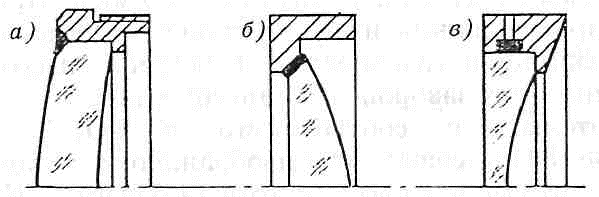
\includegraphics[width=1\textwidth]{5glue1.png}
	\label{pic:5glue1}
\end{figure}

На рис.~\ref{pic:5glue1} показаны три типовые конструкции крепления одиночных линз приклеиванием. Мениск базируется в отверстие на уступ оправы (рис.~\ref{pic:5glue1}~а). Закрепляющий клеевой шов образуется за счет заполнения клеем сопряженных фасок на линзе и оправе. Плосковыпуклая линза устанавливается фаской на клеевой шов (рис.~\ref{pic:5glue1}~б), который наносится на рабочую поверхность оправы. Плосковогнутая линза базируется на уступ оправы в осевом направлении (рис.~\ref{pic:5glue1}~в). Для образования клеевого шва в посадке линзы и оправы выполняется увеличенный до 0,5 мм зазор, так как очень тонкие слои клея теряют упругие свойства. При невозможности увеличить толщину клеевого слоя между линзой и оправой (например, для повышения точности базирования) в последней выполняется специальная канавка, которая заполняется клеем (рис.~\ref{pic:5glue1}~в).

Способ крепления оптических деталей приклеиванием имеет некоторые недостатки. Увеличение объема или усадка клеящего вещества после отвердевания могут вызвать напряжения в линзе. Поскольку зазор между линзой и оправой заполнен клеящим веществом, то при перепадах температур, из-за различных расширений этих деталей, возможно расклеивание или возникновение напряжений и деформаций. 

Большая длительность сушки клеящих веществ (от нескольких часов до суток) требует особой технологии, снижает производительность сборки. Некоторые компоненты клеящих веществ при определенных условиях (в вакууме) начинают испаряться, что может привести к загрязнению линз. Крепление, как правило, неразборное, поэтому не подлежит восстановлению. Базирование линзы в оправе на клеевой шов (рис.~\ref{pic:5glue1}~б) не обеспечивает высокую точность ее положения. Крепление линз и склеек с большой массой недостаточно надежно и требует его дублирования прижимными деталями.

Влияние ряда недостатков может быть уменьшено. Например, для повышения точности расположения линз в конструкции узла необходимо предусмотреть базирование линзы непосредственно на рабочие поверхности оправы (рис.~\ref{pic:5glue1}~а). 

В целом, несмотря на указанные недостатки, способ крепления линз приклеиванием имеет много положительных свойств, выгодно отличающих его от других, главным образом благодаря конструктивной простоте, экономичности, надежности и возможности автоматизации сборки.

\begin{flushleft}
	\textbf{Крепление резьбовым кольцом}
\end{flushleft}

Применяется как разъемное крепление отдельных линз, склеенных и составных линзовых блоков и других круглых оптических деталей. Оптическая деталь прижимается к опорному уступу оправы кольцом, имеющим наружную (или внутреннюю) резьбу, по которой оно завинчивается в оправу (рис.~\ref{pic:5ring} а). Кольцо завинчивается в оправу специальным ключом, вставляемым в специально выполненные шлицы или отверстия, а для кольца с внутренней резьбой выполняется накатка (рис.~\ref{pic:5ring}~б).

\begin{figure}[h!]
%	\caption{ Крепление линзы резьбовым кольцом:\\ а -- кольцо с наружной резьбой; б -- кольцо с внутренней резьбой}
	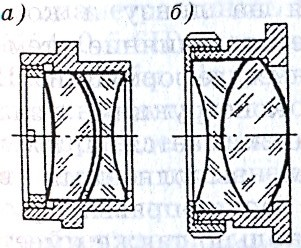
\includegraphics[width=0.5\textwidth]{5ring.png}
	\label{pic:5ring}
\end{figure}

Резьбовым кольцом рекомендуется крепить линзы с диаметром свыше 10 мм вследствие технологических трудностей выполнения внутренней резьбы в оправах меньшего диаметра, а также из-за относительно больших (по сравнению с размером линзы) габаритных размеров кольца.

Преимуществами данного способа являются обеспечение надежного разъемного крепления, простота сборки и демонтажа, отсутствие ограничений крепления линз относительно большого диаметра (до 300 мм). 

К недостаткам относятся следующие:
\begin{itemize}
\item конструкция менее технологична, чем при креплении завальцовкой или приклеиванием (так как требуется наличие дополнительной детали, крепежной резьбы в оправе, необходимо предохранять резьбовое кольцо от самоотвинчивания);
\item узел имеет увеличенные, особенно в осевом направлении, габаритные размеры; затруднена автоматизация сборки соединения;
\item невозможна юстировка линзы в оправе в процессе сборки;
\item не всегда можно обеспечить равномерный по всей окружности прижим линзы к опорному уступу оправы, что связано с перекосами кольца в резьбовом соединении, погрешностями формы и положения (отклонение от перпендикулярности) торца кольца и опорного уступа, разнотолщинностью (клиновидностью) линзы по краю;
\item при работе соединения в условиях перепада температур, из-за его жесткости могут возникнуть либо деформации линзы, либо смещения из-за уменьшения усилия прижатия или даже возникающего зазора между линзой и резьбовым кольцом.
\end{itemize}

Для устранения последних недостатков между резьбовым кольцом и линзой устанавливают пружинное кольцо (рис.~\ref{pic:5ring1}). Вследствие упругости кольца в осевом направлении достигается равномерное по всей окружности распределение давления на линзу и компенсируется влияние температурных деформаций. 

В данной конструкции узла линза поджимается к трем выступам, выполненным в опорном торце оправы. Пружинное кольцо также имеет три выступа, которые ориентированы напротив выступов оправы с помощью винта I, позволяющего   пружинному кольцу смещаться вдоль оси, но ограничивающего его разворот. В результате достигается геометрическая определенность соединения, что обеспечивает минимальные деформации при прижиме.

\begin{figure}[h!]
	\caption{ Крепление линзы с установкой пружинного кольца }
	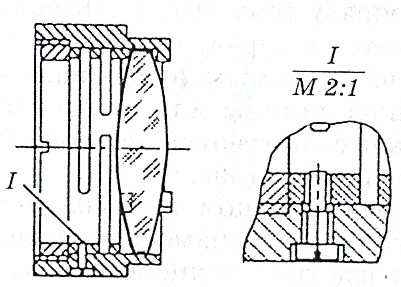
\includegraphics[width=0.65\textwidth]{5ring1.png}
	\label{pic:5ring1}
\end{figure}

\begin{flushleft}
	\textbf{Крепление проволочным кольцом}
\end{flushleft}

Этот способ применяется для закрепления линз диаметром 20-80~мм при невысоких требованиях к точности их центрирования и герметичности соединения. Он используется в основном для закрепления линз и зеркал в осветительных системах и не силовых оптических деталей (светофильтров, защитных стекол, матовых и молочных рассеивателей).

На рис.~\ref{pic:5ring2} изображены два варианта крепления линзы проволочным кольцом. В первой конструкции (рис.~\ref{pic:5ring2}~а) линза помещена между опорным уступом и выступающей частью проволочного кольца, установленного в прямоугольную кольцевую канавку оправы. Ширина канавки равна диаметру (толщине) проволоки, а глубина -- половине диаметра. Кольцо имеет вырез и изготавливается из стальной углеродистой пружинной проволоки (иногда латунной или бронзовой) диаметром 0,4--1,0мм (рис.~\ref{pic:5ring2}~в).

\begin{figure}[h!]
%	\caption{ Крепление проволочным кольцом:\\ а -- оправа с прямоугольной канавкой; б -- оправа с конической канавкой;\\ в -- проволочное кольцо }
	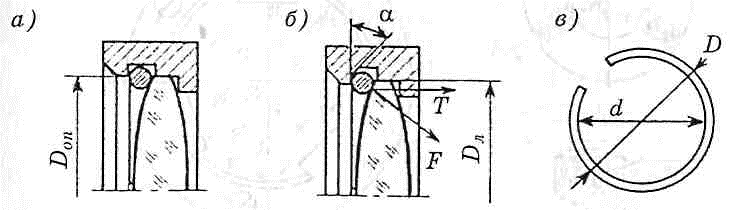
\includegraphics[width=1\textwidth]{5ring2.png}
	\label{pic:5ring2}
\end{figure}

Условие установки проволочного кольца в оправу: $ D_{min} < D_\text{оп} $, где $ D_{min} $ -- диаметр сжатого кольца; $ D_\text{оп} $ -- диаметр отверстия оправы; а условие крепления линзы в оправе: $ d_{max} < D_\text{л} $, где $ d_{max} $ -- внутренний диаметр кольца, установленного в оправу; $ D_\text{л} $ -- диаметр линзы.

Крепление проволочным кольцом конструктивно простое и технологичное. Кольцо может быть быстро установлено или снято.

Недостатком такого способа крепления является возможность смещения и перекашивания линзы в оправе, которые возникают из-за осевого зазора (обусловленного погрешностями размеров канавки, толщины линзы по краю, диаметра проволоки).

Во второй конструкции в оправе выполнена конусная канавка под проволочное кольцо (рис.~\ref{pic:5ring2}~б). В месте контакта кольца с наклонной плоскостью канавки возникает сила реакции, осевая составляющая которой прижимает линзу к опорному уступу. Для надежности соединения угол   конусной канавки должен быть меньше угла трения.

\begin{flushleft}
	\textbf{Крепление пружинящими планками}
\end{flushleft}

Крепление при помощи пружинящих планок применяется для линз, работающих в условиях перепадов температур, динамических воздействий и в случаях, когда они имеют не круглую форму боковых поверхностей. Упруго деформируясь, планки компенсируют действие факторов, ухудшающих качество соединения. Пример крепления пружинящими планками показан на рис.~\ref{pic:5planka}.

\begin{figure}[h!]
%	\caption{ Крепление пружинящими планками:\\ а -- тремя планками; б -- кольцевой планкой }
	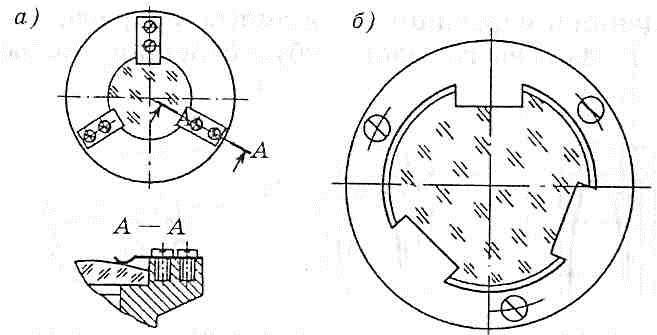
\includegraphics[width=1\textwidth]{5planka.png}
	\label{pic:5planka}
\end{figure}

Планки изготавливают из лент холоднокатаной инструментальной или пружинной стали (65Г, У8А), нейзильбера (НМцб5-20) и устанавливают через 120$^\circ$ по окружности оправы, как показано на рис.~\ref{pic:5planka}~а. Каждая планка привинчивается к оправе двумя винтами.

Для крепления линз малого диаметра три планки заменяют одним кольцом с тремя пружинящими выступами (рис.~\ref{pic:5planka}~б). Возможны и другие конструктивные реализации пружинящих планок и их соединений с оправой.

Конструкция узла характеризуется достаточной точностью и надежностью соединения линзы с оправой.

Преимуществами, которыми обладает данный способ крепления, являются следующие: возможность регулировать усилие прижима; создание упругого соединения, позволяющее компенсировать погрешность осевых размеров сопрягаемых деталей и их изменение от внешних воздействий; возможность разборки конструкции; отсутствие необходимости в специальном оборудовании и квалифицированном персонале для сборки узла. К недостаткам следует отнести: нетехнологичность конструкции, содержащей большое количество крепежных элементов; сложность автоматизации сборки; невозможность юстировки в процессе сборки.

\begin{flushleft}
	\textbf{Крепление накладным кольцом}
\end{flushleft}

Данный способ применяют для крепления крупногабаритных линз, а также других круглых оптических деталей (защитных стекол, зеркал) с диаметром, превышающим 200-300~мм. Крепление накладным кольцом относится к индивидуальным способам крепления. Его реализация зависит от конкретных геометрических параметров оправы и линзы, их допустимых отклонений, а также от температурного режима работы соединения.

Схема крепления показана на рис.~\ref{pic:5nakladnoe}. Линзу устанавливают в оправу на фаску опорного буртика, выполненную под углом 135$^\circ$ или по касательной к рабочей поверхности линзы, к которому она прижимается накладным кольцом. Рабочая поверхность прижимного кольца тоже выполняется по касательной к поверхности линзы и крепится к оправе болтами Для компенсации погрешностей изготовления соответствующих размеров оправы, линзы и накладного кольца и их изменений при отклонениях температуры между контактирующими поверхностями линзы и кольца устанавливается упругая прокладка.

\begin{figure}[h!]
	\caption{ Крепление линзы накладным кольцом }
	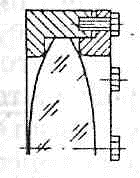
\includegraphics[width=0.3\textwidth]{5nakladnoe.png}
	\label{pic:5nakladnoe}
\end{figure}
 
Для центрирования линзы в оправе могут применяться вкладыши (например, полоски фольги толщиной 0,005 мм), которые устанавливают в зазор между посадочным отверстием оправы и линзой. Иногда линзу центрируют в оправе сдвигом (наклоном) винтами с последующей фиксацией герметиком.
Для компенсации возможных пережатий или смещений линзы при перепадах температуры в ряде случаев между диаметрами линз и отверстиями оправы устанавливают термокомпенсаторы.

Данный способ крепления обладает рядом недостатков: трудоемкость сборки узла из-за подгонки прижимного кольца; увеличенные габаритные размеры конструкции, так как накладное кольцо выступает за пределы оправы; невозможность автоматизации сборки.

К преимуществам способа следует отнести: надежность крепления; возможность частичной юстировки положения линзы относительно оправы; возможность применения термокомпенсаторов.

\begin{flushleft}
	\textbf{Специальные (нетрадиционные) способы крепления}
\end{flushleft}

К этим способам крепления линз относятся, например: крепление линзы в оправе стопорными винтами (или привинчивание линзы винтами к оправе через просверленные в ней отверстия); заливка линзы в оправе зубным или глетоглицериновым цементом; заформовка линзы в оправу из термопластичных пластмасс; обжатие линзы <<хомутовыми>> или разъемными оправами. На рис.~\ref{pic:5obj} изображена конструкция проекционного объектива, линзы которого закреплены в разъемной пластмассовой оправе.

\begin{figure}[h!]
	\caption{ Проекционный объектив }
	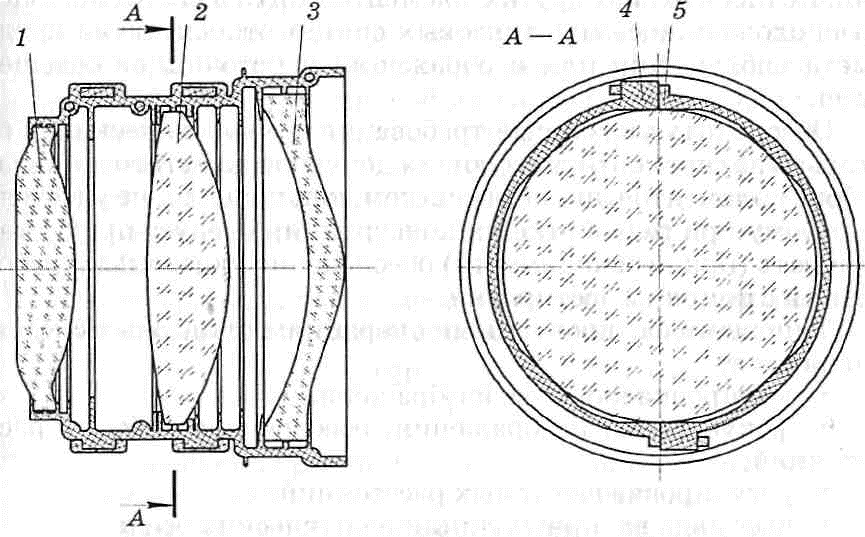
\includegraphics[width=1\textwidth]{5obj.png}
	\label{pic:5obj}
\end{figure}

\section{Конструкции линзовых систем}

К линзовым системам оптических приборов относятся объективы, окуляры, оборачивающие системы, системы смены увеличения, конденсоры и коллекторы. Как правило, эти функциональные устройства состоят из нескольких или большого количества линз и склеенных блоков (в некоторых из них содержатся также и другие оптические детали: сетки, зеркала, защитные стекла, светофильтры, рассеиватели).

В зависимости от способа установки и сопряжения этих оптических деталей с несущим элементом (корпусом) устройства конструкции линзовых систем подразделяют на насыпные, насыпные в оправах, резьбовые, комбинированные и специальные. 

В насыпных конструкциях линзы (и прочие детали) устанавливаются последовательно друг за другом (насыпаются) непосредственно в корпусную деталь. Необходимые воздушные промежутки между компонентами выдерживаются здесь с помощью промежуточных колец (рис.~\ref{pic:5condensor}) либо точным изготовлением их конструктивных параметров (диаметров и фасок, рис.~\ref{pic:5photoobj}). Точность центрировки компонентов системы обуславливается погрешностями центрировки самих линз, зазорами их посадок в корпус, наклонами из-за перекоса опорного торца корпуса, клиновидностями промежуточных колец или биением опорных фасок, а также несоосностью посадочных рабочих поверхностей корпуса (рис.~\ref{pic:5condensor}~б,~в).

\begin{figure}[h!]
	\caption{ Насыпные с промежуточными кольцами конструкции конденсоров }
	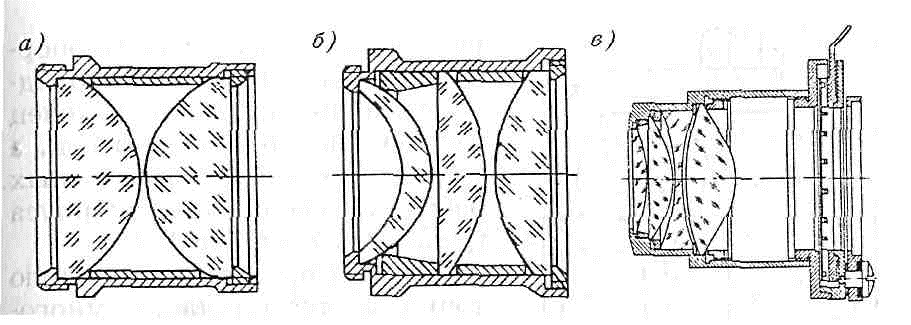
\includegraphics[width=1\textwidth]{5condensor.png}
	\label{pic:5condensor}
\end{figure}

\begin{figure}[h!]
	\caption{ Насыпная без промежуточных колец, конструкция фотообъектива }
	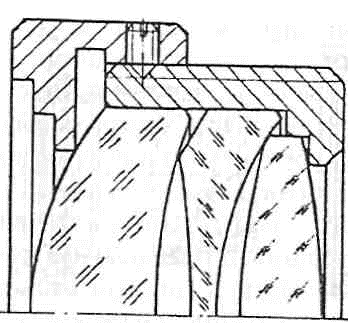
\includegraphics[width=0.4\textwidth]{5photoobj.png}
	\label{pic:5photoobj}
\end{figure}

Так как обеспечить высокую точность центрировки многокомпонентной линзовой системы из-за перечисленных погрешностей весьма сложно, а юстировка центрировки при насыпной конструкции затруднена или невозможна, то ее используют обычно в конструкциях осветительных систем (конденсоров, коллекторов), окуляров и относительно простых объективов. Данная конструкция не используется также в случаях, когда линзы системы существенно отличаются друг от друга по световому диаметру.

Насыпная конструкция (особенно без промежуточных колец) является наиболее технологичной, так как содержит минимально возможное количество деталей. Поэтому наблюдается устойчивая тенденция все более частого ее использования в конструкциях линзовых узлов приборов.

Насыпная в оправах конструкция отличается от предыдущей тем, что линзы и компоненты вначале закрепляются тем или иным способом (чаще всего завальцовкой или приклеиванием) в своих оправах, а затем устанавливаются последовательно в корпусную деталь (рис.~\ref{pic:5photoobj1},~\ref{pic:5photoobj2}).

\begin{figure}[h!]
	\caption{ Насыпная в оправах конструкция фотообъектива }
	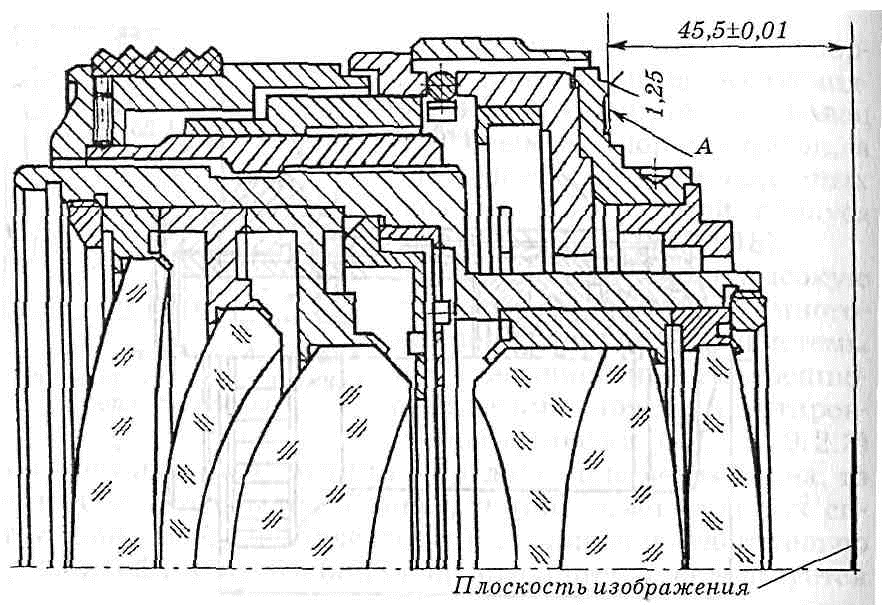
\includegraphics[width=1\textwidth]{5photoobj1.png}
	\label{pic:5photoobj1}
\end{figure}

\begin{figure}[h!]
	\caption{ Фотографический проекционный объектив }
	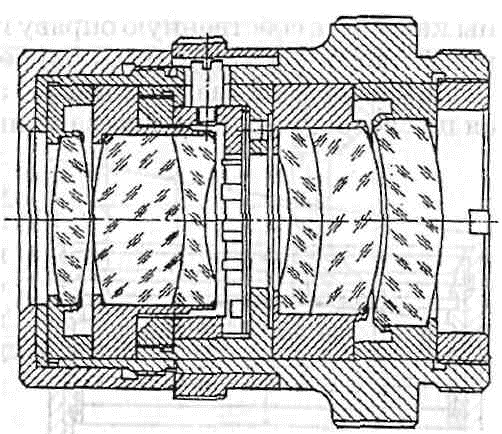
\includegraphics[width=1\textwidth]{5photoobj2.png}
	\label{pic:5photoobj2}
\end{figure}

Воздушные промежутки между компонентами обеспечиваются точным выполнением соответствующих конструктивных размеров оправ компонентов (при необходимости воздушный промежуток может юстироваться). Точность центрировки компонентов системы обуславливается погрешностями расположения центров кривизны их поверхностей и неперпендикулярностью плоских поверхностей относительно базовых осей оправ, зазорами посадок оправ в корпус, наклонами оправ из-за перекоса опорного торца корпуса и клиновидности оправ, несоосностью посадочных рабочих поверхностей корпуса (рис.~\ref{pic:5photoobj1}).

Насыпная в оправах конструкция применяется обычно при конструировании многокомпонентных фотобъективов (рис.~\ref{pic:5photoobj1}), микрообъективов, проекционных и фотограмметрических объективов (рис.~\ref{pic:5photoobj2}), зеркально-линзовых объективов.

На рис.~\ref{pic:5photoobj2} представлена конструкция многолинзового проекционного объектива, компоненты которого завальцованы каждый в собственную оправу и установлены в общий корпус. Силовое замыкание выполняется резьбовым кольцом.

В резьбовых конструкциях линзы и компоненты закрепляются каким-либо способом в своих оправах, которые соединяются по резьбе с корпусной деталью (рис.~\ref{pic:5photoobj3}).

\begin{figure}[h!]
	\caption{ Резьбовая конструкция оправы фотообъектива }
	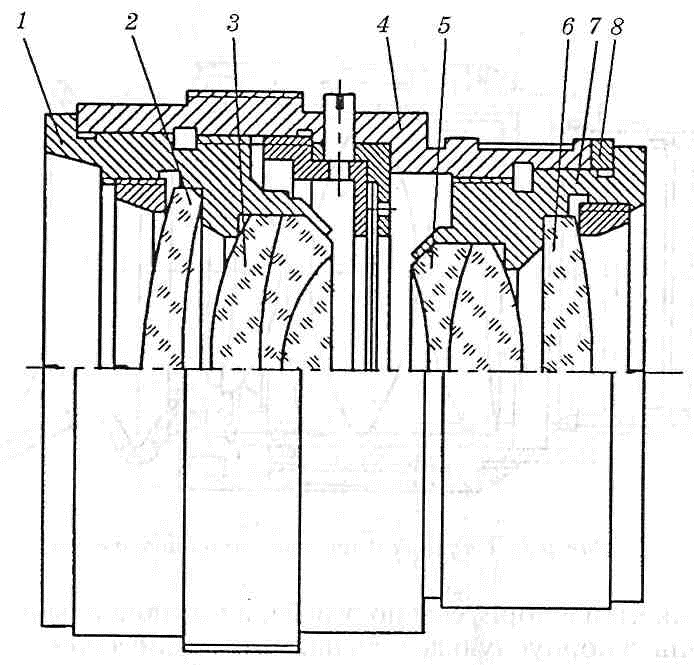
\includegraphics[width=0.8\textwidth]{5photoobj3.png}
	\label{pic:5photoobj3}
\end{figure}

Резьбовая конструкция является наименее технологичной из рассмотренных выше, так как более трудоемка при изготовлении и сборке, поэтому в настоящее время используется относительно других гораздо реже. В этой конструкции практически невозможно осуществлять юстировку центрировки компонентов системы.

В комбинированных конструкциях компоненты линзовых, систем сопрягаются с несущей (корпусной) деталью различными способами: непосредственно устанавливаются в корпус, насыпаются в оправах или их оправы соединяются с корпусом по резьбе (рис.~\ref{pic:5helios}).

На рис.~\ref{pic:5helios} изображена конструкция фотообъектива <<Гелиос-44Н>>, компоненты 1 и 2 которого закреплены в оправе, соединяемой с корпусом по резьбе, а компоненты 3 и 4 установлены в корпусную деталь насыпным способом. 

На рис.~\ref{pic:5Canon} изображена конструкция фотообъектива Canon, в которой присутствуют рассмотренные ранее различные конструкции крепления линз.

В специальных конструкциях линзы и компоненты устанавливаются и закрепляются в корпусной детали нетрадиционным способом. На рис.~\ref{pic:5obj} представлена конструкция проекционного объектива, линзы которого (две из них 1 и 3 выполнены из полистирола, а третья 2 -- из силикатного стекла) установлены в призматических канавках литой пластмассовой общей оправы, выполненной из двух цилиндрических половинок 4, 5. Крепление линз осуществляется обжимом их половинками оправы, вставленной в корпусную деталь. Благодаря упругости тонких буртиков призматических канавок производится беззазорное сопряжение линз с оправой. Точность расположения линз достигается точным литьем элементов оправы.

Более подробные сведения о конструкциях тех или иных видов и типов линзовых систем: объективов (например, фотографических, телескопических, проекционных, микроскопических, зеркально-линзовых), окуляров, осветительных систем изложены в справочниках и специальной литературе.
\begin{landscape}
	
	\begin{figure}[h!]
		\caption{ Фотообъектив <<Гелиос-44Н>> }
		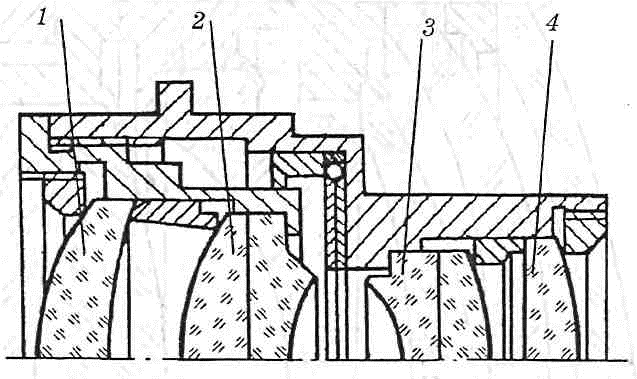
\includegraphics[width=0.45\textwidth]{5Helios.png}
		\label{pic:5helios}
	\end{figure}
	
	\begin{figure}[h!]
		\caption{ Фотообъектив Canon }
		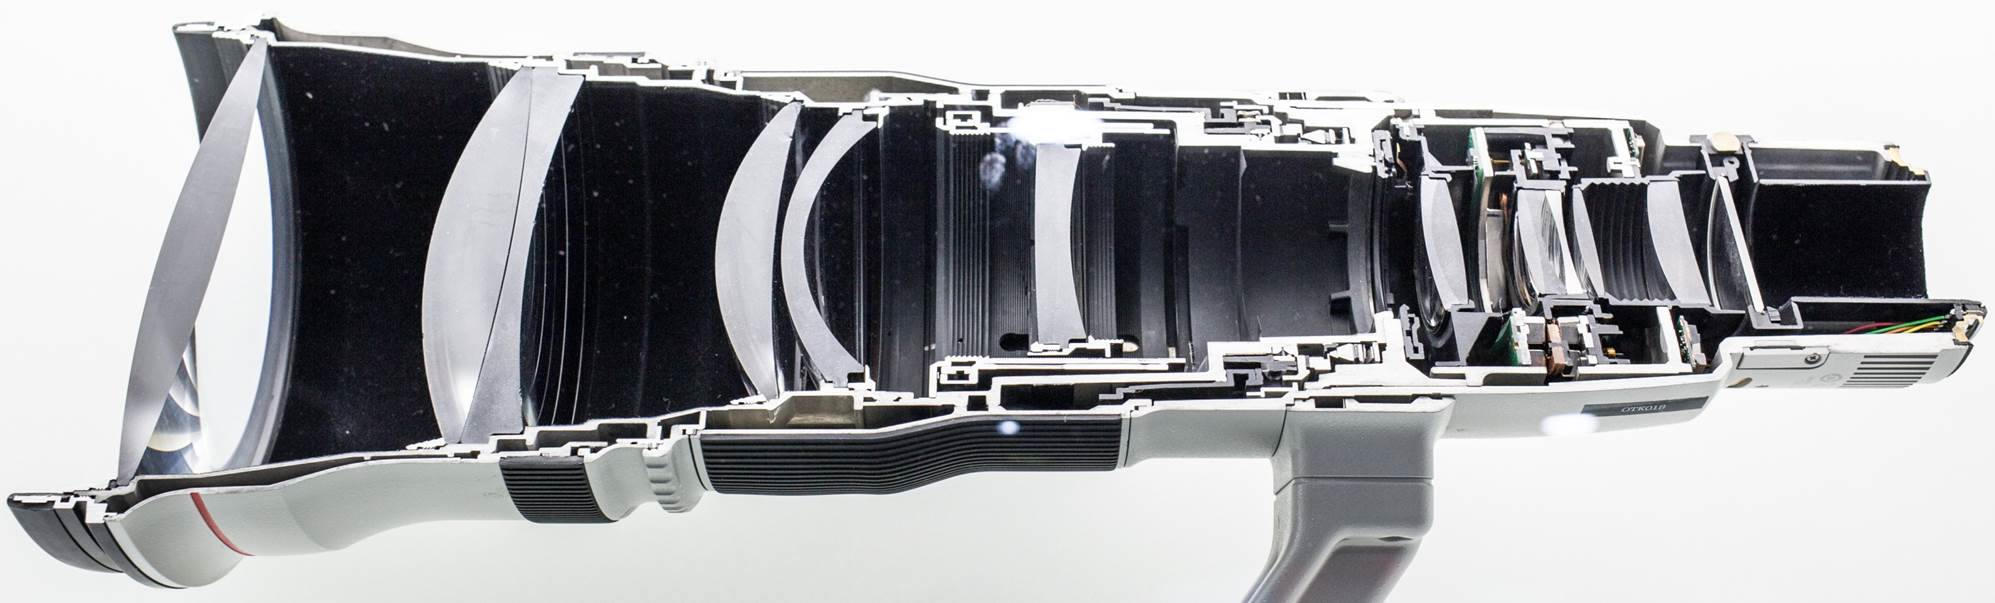
\includegraphics[width=0.9\textwidth]{5Canon.png}
		\label{pic:5Canon}
	\end{figure}
\end{landscape}


\chapter{Призмы, зеркала и способы их крепления}
\section{Призмы}

\textit{Призмами} называют оптические детали или оптические системы деталей (объединенные в единый блок) с плоскими рабочими поверхностями (гранями) на которых происходит преломление или отражение оптического излучения.

В оптических приборах призмы применяют в следующих целях:
\begin{itemize}
\item для изменения хода лучей, направления оптической оси системы и направления линии визирования;
\item оборачивания изображения;
\item уменьшения габаритных размеров системы;
\item разделения или объединения пучков лучей, полей или изображений;
\item вращения  изображения  или  компенсации  поворота изображения;
\item сканирования изображения или модулирования излучения;
\item разложения света в спектр;
\item поляризации света;
\item юстировки и аттестации приборов, создания измерительных баз.
\end{itemize}

Призмы подразделяют обычно на две группы: отражательные и спектральные. К группе спектральных относят также поляризационные, модулирующие и отклоняющие излучение призмы на основе физических эффектов в их материалах при воздействии на них электрических или магнитных полей.
Самой многочисленной группой являются отражательные призмы, на примере которых рассмотрим некоторые аспекты их конструирования.По своему действию на световой пучок отражательные призмы подобны зеркалам, однако в ряде случаев призмы более эффективны, чем зеркала.

Преимущества отражательных призм по отношению к зеркалам:
\begin{itemize}
\item углы между гранями призмы неизменны, тогда как углы между зеркалами должны регулироваться с большой точностью при сборке и могут разъюстироваться в процессе эксплуатации;
\item потери света у призм от граней с полным внутренним отражением равны нулю, тогда как при отражении от поверхностей зеркал потери довольно велики; кроме того, отражающие покрытия зеркал с течением времени могут портиться;
\item конструкция крепления призм в оправах, как правило, проще, чем у системы зеркал, и обладает меньшими габаритными размерами;
\item для некоторых призм нет эквивалентных зеркальных систем (например, для призмы Дове, полупенты, некоторых видов спектральных призм).
\end{itemize}
 
Замена отражательных призм зеркалами целесообразна в случаях:
\begin{itemize}
\item когда имеют значение масса прибора, так как зеркала значительно легче призм; 
\item при высокой стоимости оптического материала;
\item для достижения требуемого качества изображения, так как призмы являются источниками хроматических и других аберраций, особенно в случаях их работы в сходящемся пучке лучей.
\end{itemize}

Рабочие и нерабочие поверхности (грани) призмы представляют собой плоскости. Рабочие поверхности подразделяют на преломляющие, через которые световой пучок входит в призму или выходит из нее, и отражательные, от которых пучок отражается при прохождении внутри призмы.

Число рабочих граней и взаимное их расположение определяют ход пучка внутри призмы и все преобразования пучка, которые при этом происходят.
Если осевой луч проходит внутри призмы в одной плоскости, то такую призму называют плоской. Если осевой луч идет в двух плоскостях, такая призма называется пространственной.

Сечение призмы плоскостью, в которой проходит осевой луч пучка, называется главным, сечением, призмы; у плоских призм одно главное сечение, у пространственных главных сечений столько, сколько плоскостей, в которых проходит осевой луч.

Отражательные призмы подразделяют на простые (их называют также одинарными), выполненные из одной заготовки материала, и составные (призменные блоки), представляющие собой комбинации из двух или большего числа простых призм, объединенных в единый блок с помощью склейки или закрепления в оправе (рис.~\ref{pic:6prism}).

\begin{figure}[h!]
	\caption{ Отражательные призмы с одним (а, в) и двумя отражениями (б) }
	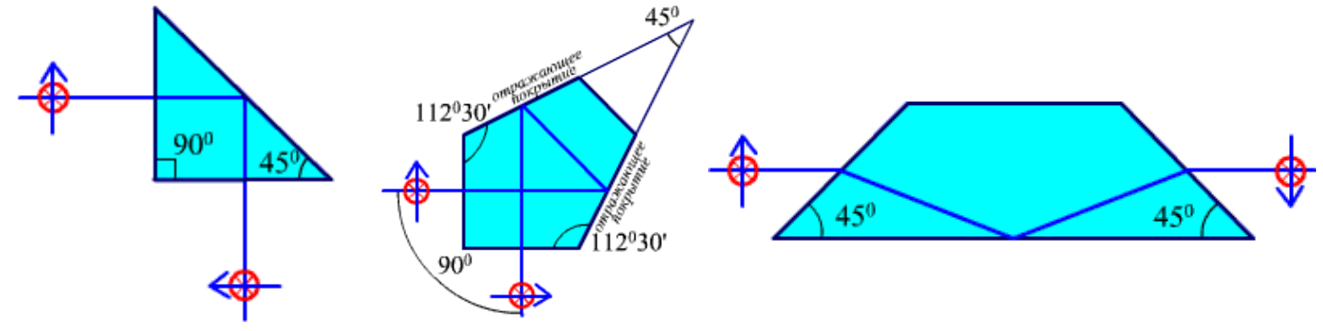
\includegraphics[width=1\textwidth]{6prism.png}
	\label{pic:6prism}
\end{figure}

Основными целевыми характеристиками отражательных призм являются: угол отклонения светового пучка, линейное смещение пучка, оборачивание изображения, степень возможности разделения или совмещения пучков лучей.

Углом отклонения называется угол между направлениями осевого луча до и после призмы, причем промежуточные отклонения луча внутри призмы во внимание не принимаются.

Линейным, смещением пучка называют расстояние между параллельными направлениями осей падающего на призму и выходящего из призмы пучка лучей. Если это расстояние равно нулю (направления осей падающего и прошедшего пучка совпадают), то такие призмы называют призмами прямого зрения (видения).

Оборачивание изображения зависит от числа отражающих граней и их расположения в пространстве.

Плоские призмы с четным числом отражающих граней дают прямое изображение. При наклоне такой призмы в главной плоскости выходящий пучок лучей не отклоняется.

Плоские призмы с нечетным числом отражающих граней дают зеркальное изображение предмета. При наклоне их в плоскости главного сечения лучи отклоняются на двойной угол.

Для оборачивания изображения в плоскости, нормальной к главному сечению, одна из отражающих граней призмы заменяется крышей, которая представляет собой две отражающие поверхности, образующие двугранный угол 90$ ^\circ $, симметрично расположенные относительно главного сечения призмы (рис.~\ref{pic:6roof}).

\begin{figure}[h!]
	\caption{ Призмы с крышей }
	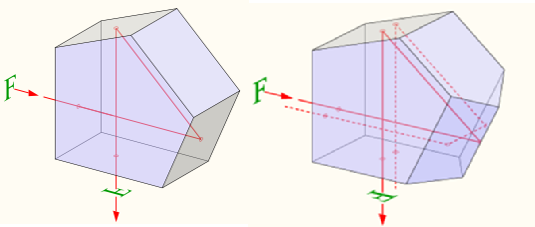
\includegraphics[width=1\textwidth]{6roof.png}
	\label{pic:6roof}
\end{figure}

Степень возможности разделения или объединения пучка лучей призмой (призменным блоком) определяется способностью разделять (объединять) пучок на две, три или более составляющих (как правило, это составные призмы типа призмы-куб, Кестерса, цветоделительной).

Типовые простые призмы, имеют условное обозначение в виде двух букв и числа, разделенных знаком тире.

Первая буква указывает число отражающих граней призмы (А -- одно отражение, Б -- два, В -- три), вторая --- характер ее конструкции (Р --  равнобедренная, П -- пентапризма\footnote{Пентапризма~-- общее название оптического устройства, служащее для поворота оси светового потока на 90$^\circ$ и удлинения его пути за счёт двух и более отражений от зеркальных поверхностей, обеспечивает минимальные внешние габаритные размеры всей сложной оптической системы}, У~-- полупента, С~-- ромбическая, Л~-- призма Лемана). Число обозначает угол отклонения осевого луча в градусах. При этом крыша считается за одну грань. Обозначается крыша индексом <<К>> у первой буквы. Для пространственных призм указываются углы отклонения в соответствующих плоскостях по ходу луча.

Типовые составные призмы, имеют другие условные обозначения. Буквой обозначают тип призмы (например, А -- Аббе-призма, К -- куб-призма, Б -- башмачная, П -- Пехана-призма), цифрой -- угол отклонения.

Составные призмы применяются в тех случаях, когда простые призмы не могут обеспечить необходимые целевые характеристики или не могут быть установлены в сходящемся пучке лучей (так как разворачиваются в наклонную плоскопараллельную пластинку и вносят большие аберрации) либо когда требуется уменьшить габаритные размеры системы.

На рис.~\ref{pic:6sostav} и ~\ref{pic:6spatial} представлены составные и светоделительные призмы.
\begin{figure}[h!]
	\caption{ Составные призмы: а, б -- башмачные, в -- Пехана, г -- Аббе }
	\includegraphics[width=1\textwidth]{6sostav.png}
	\label{pic:6sostav}
\end{figure}

\begin{figure}[h!]
	\caption{ Пространственные призменные системы }
	\includegraphics[width=0.7\textwidth]{6spatial.png}
	\label{pic:6spatial}
\end{figure}

На рис.~\ref{pic:6spatial} приведены составные пространственные призмы, использующиеся как оборачивающие призменные системы --- призменные системы Малафеева-Порро первого (рис.~\ref{pic:6spatial}~а) и второго рода (рис.~\ref{pic:6spatial}~б).

\textbf{Конструктивные параметры} призм, так же как и для линз, подразделяют на \textit{расчетные} и \textit{конструкторские}.

К \textit{расчетным параметрам} относят: оптические характеристики и показатели качества материала призмы, ее световые диаметры $ O_\varnothing $ на рабочих поверхностях, длину хода луча в призме $ l $, допустимые значения погрешностей изготовления рабочих оптических поверхностей (погрешности формы $ N , \Delta N$), погрешности углов призмы, влияющие на качество изображения, пирамидальность $ \pi $, вид оптических покрытий, а также (при необходимости) значения допустимой фокусности $ f_{min} $ и предел разрешения $ \varepsilon $. Эти данные определяются при габаритном, аберрационном и светотехническом расчетах оптической системы.

К \textit{конструкторским параметрам} относят габаритные размеры призмы (которые зависят от типа призмы, ее световых диаметров, запаса для крепления, юстировки), параметры фасок на ребрах и углах, допуски на углы, не влияющие на качество изображения, класс чистоты рабочих полированных поверхностей, шероховатость рабочих и нерабочих поверхностей, покрытия матовых поверхностей. Эти параметры получают в процессе разработки ее окончательной конструкции.

\section[Узлы крепления одиночных призм и призменных систем]{Узлы крепления одиночных призм и\\ призменных систем}

Призмы и призменные системы, применяемые в оптических приборах, характеризуются многообразием форм и размеров. В связи с этим существует большое количество разнообразных конструкций узлов крепления одиночных призм и составных блоков призм, достаточно полно рассмотреть которые в объеме курса лекций не представляется возможным. Рассмотрим некоторые из них.

Типовые способы крепления одиночных призм обычно классифицируют по виду основной детали, осуществляющей прижим (замыкание) призмы к рабочей поверхности оправы. Поэтому различают крепление призм накладкой, прижимными планками (лапками), угольниками, установочными винтами, пружинами, специальными деталями. Для крепления призм также используют клеи и замазки.

При разработке узла крепления любой призмы необходимо соблюдать следующие рекомендации:
\begin{enumerate}[leftmargin=*]
\item Для обеспечения точности положения призмы и исключения деформаций изгиба рабочая плоскость (плоскости) оправы должна быть чисто обработана ($ R_a $=1,25 $ \div $ 3,2 мкм) и иметь высокую степень плоскостности. При относительно больших размерах призмы на рабочей поверхности делают выборку (для выполнения принципа геометрической определенности соединения), и тогда призма базируется на два выступа по краям, либо применяют базирование на три опорные площадки.
\item Чтобы не нарушать требуемые условия преломления и отражения на рабочих гранях призмы, рекомендуется базировать призму на нерабочую грань. При базировке призмы на рабочую грань (грани) сопряжение ее с оправой должно происходить за пределами светового диаметра. При необходимости использовать для крепления или ориентации призмы грани, работающие с полным внутренним отражением, необходимо минимизировать площадь контакта между гранью и деталью крепления, например, реализовать контакт между указанными элементами по линии или точечный контакт.
\item Не допускается контакт крепежных элементов с ребрами призмы во избежание выколок стекла.
\item Между призмой и крепежным элементом (за исключением пружины) следует ставить эластичную прокладку из пробки, картона, паронита, текстолита, противоосыпочной резины или силиконового герметика, которая компенсирует погрешности размеров деталей, равномерно распределяет усилие прижима на большую площадь, предотвращает появление температурных деформаций и смещений.
\item Сопряжение призмы с рабочей поверхностью оправы отнимает три степени свободы. Базирование призмы двумя рабочими плоскостями на две плоскости оправы отнимает пять степеней свободы. Оставшиеся степени свободы призмы отнимаются соответствующим количеством ориентирующих планок.
\item Для юстировки призм следует предусматривать в конструкции их узлов возможность выполнения необходимых юстировочных подвижек.
\item Крепление склеенных призменных блоков осуществляется за одну из них, а именно -- базовую, в качестве которой выбирается наиболее массивная призма. Приклеиваемые к ней другие призмы должны иметь меньшую массу и по возможности не касаться элементов оправы.
\end{enumerate}

\begin{flushleft}
	\textbf{Крепление накладкой}
\end{flushleft}

Применяется для любых призм, имеющих параллельное расположение нерабочих граней (прямоугольная призма, пентапризма, призма Шмидта). Например, прямоугольная призма установлена нерабочей гранью на плоскость оправы (рис.~\ref{pic:6nakladka}). К оправе 1 призма прижимается накладкой~3 через эластичную прокладку 2. Накладка крепится винтами к двум стойкам, жестко соединенным с оправой. Ориентация призмы вдоль плоскости оправы выполняется при помощи трех ограничительных (ориентирующих) планок~4.

\begin{figure}[h!]
	\caption{ Крепление прямоугольной призмы накладкой }
	\includegraphics[width=0.8\textwidth]{6nakladka.png}
	\label{pic:6nakladka}
\end{figure}

Крепление накладкой характеризуется универсальностью, относительной простотой оправы и простотой сборки, надежностью, реализуется принцип полного внутреннего отражения на отражающих гранях, возможна юстировка призмы в оправе.

\begin{flushleft}
	\textbf{Крепление угольниками}
\end{flushleft}

Этот способ основан на использовании в узле крепления нескольких угольников различной формы (Г-образных, Z-образных). Дополнительно к угольникам применяют ориентирующие планки. Типовые конструкции крепления данным способом показаны на рис.~\ref{pic:6ugol}.

\begin{figure}[h!]
	\caption{ Крепление призм угольниками }
	\includegraphics[width=0.8\textwidth]{6ugol.png}
	\label{pic:6ugol}
\end{figure}

Пентапризма (рис.~\ref{pic:6ugol}~а) прижимается к плоскости оправы двумя угольниками 1. Усилие прижима призмы создается в результате деформации эластичных прокладок, помещенных между призмой и угольниками. Ориентирование призмы на плоскости оправы произведено при помощи угловой планки 2, которая контактирует с преломляющими гранями призмы. После установки призмы в рабочее положение планка фиксируется штифтами.

На рис.~\ref{pic:6ugol}~б показан пример крепления угольниками прямоугольной призмы. Особенностью данной конструкции является то, что в нерабочих гранях закрепляемой призмы выполнены прямоугольные канавки. Здесь для прижима призмы к основанию оправы используются элементы канавок, через которые низкими угольниками 1 призма прижимается к основанию. Ограничение бокового перемещения призмы обеспечивается ориентирующими планками 2. Планки винтами крепятся к основанию оправы.

Этот способ крепления призм получил довольно широкое практическое применение благодаря простоте и надежности. Недостатками являются усложнение технологии изготовления снабженных канавками призм и возможность их скола при креплении.

Крепление прижимными планками. Данный способ крепления применяется для крепления сложных призм (призм с крышей, склеенных блоков), когда необходимо применить нетрадиционное базирование призмы, например -- прямоугольная призма устанавливается на гипотенузную грань.

Характерным для этого способа крепления является более сложная конструкция оправы или прижимных планок. Как правило, оправа охватывает призму с трех сторон. При этом одна (или две) поверхности базирующие, а на других - закрепляются прижимные планки. Прижимные планки бывают различными по конструкции: в виде лапок, угольников, пластин, согнутых пластин и т. п. На рис. 7 а показано крепление прямоугольной призмы с крышей. Призма установлена на катетную грань между стенками оправы с гарантированным зазором, который при необходимости выбирается эластичной прокладкой. Две пары прижимных планок ограничивают перемещение призмы в продольном и вертикальном направлениях.

На рис.~\ref{pic:6planka}~б показано крепление прямоугольной призмы, установленной гипотенузной гранью на базирующую поверхность оправы. Четыре прижимные планки привинчены к вертикальным стенкам оправы. Контакт планок с призмой выполнен по краевым зонам ее входной и выходной поверхностей. Планки выполняют упругими, либо между ними и призмой устанавливают эластичные прокладки.

\begin{figure}[h!]
	\caption{ Крепление призм прижимными планками }
	\includegraphics[width=1\textwidth]{6planka.png}
	\label{pic:6planka}
\end{figure}

Недостатком этого способа крепления является неуниверсальность и сложность деталей узла. В частности, требуется изготавливать сложные формы оправ и оригинальные прижимающие планки для каждого типа призм. Базирование на рабочие поверхности может нарушить требуемые условия отражения и вызвать воздействие недопустимых усилий. Юстировка призмы практически невозможна.

Крепление установочными винтами. Этот способ крепления рекомендуется применять для закрепления относительно больших призм с размером грани, превышающим 30 мм, когда требуется распределить усилие прижима равномерно по всей грани.

В варианте крепления пентапризмы, показанном на рис.~\ref{pic:6screw}, замыкание призмы на основание осуществляется тремя установочными винтами. Между призмой и винтами помещены эластичная и металлическая прокладки. Размеры пластин соответствуют размерам грани призмы. Металлическая пластина позволяет равномерно распределить усилие прижима по всей грани, а также предотвращает возникновение повреждений призмы при сборке. 

В свою очередь, эластичная прокладка компенсирует погрешности формы металлической пластины и изменение размеров деталей при изменении температуры. Смещения и повороты призмы вдоль основания оправы ограничиваются двумя ориентирующими планками, закрепленными на основании оправы.

\begin{figure}[h!]
	\caption{ Крепление пентапризмы установочными винтами }
	\includegraphics[width=0.9\textwidth]{6screw.png}
	\label{pic:6screw}
\end{figure}

Данная конструкция характеризуется простотой используемых деталей и надежностью фиксирования призмы. Установочными винтами можно регулировать усилие прижима. Призма защищена от внешних воздействий корпусом оправы с трех сторон.

В конструкции необходимо предусмотреть защиту от самоотвинчивания установочных винтов.

\begin{flushleft}
	\textbf{Крепление пружинами}
\end{flushleft}

Пружина как элемент крепления широко используется для закрепления призм, имеющих относительно много рабочих граней (например, прямоугольная призма с крышей). Это позволяет упростить конструкцию узла крепления. Вместе с этим пружины целесообразно использовать для прижима призмы при ее установке непосредственно в корпусную деталь прибора. В узлах крепления призм применяют пружины различных форм: тарельчатые, плоские, изогнутые, которые обычно изготавливают из пружинной стали 30X13, 65Г, У8А.

На рис.~\ref{pic:6spring} изображено крепление пружиной прямоугольной призмы с крышей. К специальной фаске на ребре призмы (90$ ^\circ $) приклеивается цилиндрический шарнир. Шарнир установлен в паз, который выполнен в корпусной детали. Вместе они образуют направляющую вращения, относительно которой можно выполнять регулировочные наклоны призмы.

Силовое замыкание призмы осуществляется изогнутой пластинчатой пружиной с закругленными краями, которые опираются на грани крыши. Регулировка усилия пружины выполняется двумя установочными винтами. При этом сила давления на призму, работающую при ударных нагрузках должна быть в 15-20 раз больше массы призмы, при работе в лабораторных приборах~-- от двух до пяти раз. Для ограничения перемещения призмы в плоскости, перпендикулярной к главному сечению (вид А-А), между призмой и крышкой корпуса установлена пластина с эластичной прокладкой.

\begin{figure}[h!]
	\caption{ Крепление прямоугольной призмы с крышей пружиной }
	\includegraphics[width=0.7\textwidth]{6spring.png}
	\label{pic:6spring}
\end{figure}

Данная конструкция крепления позволяет выполнять угловые юстировочные подвижки призмы. Для этого при помощи двух установочных винтов изменяют усилие прижима пружины к призме. Наличие пружины обеспечивает устойчивость крепления к воздействию вибраций, толчков, а также компенсирует воздействие на узел крепления изменений температуры.

К недостаткам следует отнести необходимость физического контакта пружины с рабочими отражающими гранями призмы, который может привести не только к повреждению призмы при сборке и юстировке, но и к исчезновению эффекта полного внутреннего отражения. Поэтому площадь контакта должна быть минимальной, по возможности вне зоны светового пучка.

На рис.~\ref{pic:6planspring} показан фрагмент крепления призмы плоской пружиной. Здесь призма установлена нерабочей гранью на плоское основание оправы. Боковое перемещение призмы ограничено установочными планками. Выставленное положение призмы фиксируется пластинчатой пружиной, которая осуществляет давление на перемещающийся во втулке стержень. Для равномерного распределения усилия прижима между стержнем и гранью призмы помещены металлическая и эластичная прокладки.

\begin{figure}[h!]
	\caption{ Крепление призмы, плоской пружиной }
	\includegraphics[width=0.6\textwidth]{6planspring.png}
	\label{pic:6planspring}
\end{figure} 

\begin{flushleft}
	\textbf{Крепление приклеиванием}
\end{flushleft}

Одной из конструктивных особенностей призм является сложность формы, отличающая их от круглых оптических деталей. Поэтому крепление призм приклеиванием, особенно имеющих небольшую массу, экономически существенно выгоднее других способов крепления.

Рассмотрим пример крепления прямоугольной призмы, у которой для использования эффекта полного внутреннего отражения, отражающая гипотенузная грань должна быть полностью свободна. Это требование наиболее просто можно обеспечить приклеиванием призмы к оправе по ее нерабочей грани (рис.~\ref{pic:6glue}). Здесь призма приклеена к боковой поверхности оправы в виде угольника, который может юстироваться с помощью винтов. Приклеивание осуществляется либо по всей поверхности сопряжения, либо по его периметру, либо по его части, например по цилиндрическому пятну 1 выборки в оправе, куда заливается герметик или другое клеящее вещество.

\begin{figure}[h!]
	\caption{ Призма, приклеенная к оправе одной гранью }
	\includegraphics[width=0.8\textwidth]{6glue.png}
	\label{pic:6glue}
\end{figure} 

Недостатком такого крепления является ограничение массы приклеиваемой призмы. Клеящий слой не позволяет обеспечить надежное скрепление массивной призмы и оправы, особенно при консольном положении призмы.

Конструкция оправы (рис.~\ref{pic:6gluescrew}) позволяет осуществить надежное крепление массивной прямоугольной призмы приклеиванием. В данной конструкции высокие требования к положению призмы 1 обеспечиваются подготовкой базирующих поверхностей оправы 4. Призма установлена на краевые зоны преломляющих граней и прижимается к базовым плоскостям оправы упорным винтом 4 через пластину 2. Зазоры между оправой и призмой заполняются клеящим веществом 5. После затвердевания клея винт 4 можно удалить, а образовавшуюся пустоту заполнить клеем. Для исключения потери эффекта полного внутреннего отражения пластина 2 должна иметь выборку, соответствующую световому размеру пучка лучей на гипотенузной грани, в противном случае на гипотенузную грань призмы следует нанести зеркальное отражающее покрытие с соответствующей защитой.

\begin{figure}[h!]
	\caption{ Крепление призмы приклеиванием со вспомогательным винтом }
	\includegraphics[width=0.35\textwidth]{6gluescrew.png}
	\label{pic:6gluescrew}
\end{figure}

Клеящие материалы, которые рекомендуется применять для крепления призм к оправам -- это различные герметики, компаунды, эпоксидные смолы.
Оправы для крепления призм приклеиванием, как правило, изготавливают из алюминиевых сплавов с последующим чернением (анодным оксидированием).
Специальные способы крепления. К таким способа относят крепление с использованием специальных крепящих деталей, либо комбинации крепящих деталей различных видов, а также крепление зажимом призм с деформированием элементов оправы, крепление формовкой призм в пластмассовые оправы, постановкой их на оптический контакт.

\begin{flushleft}
	\textbf{Конструкции узлов крепления призменных систем}
\end{flushleft}

Призмы, представляющие собой систему из двух или большего числа простых типовых призм, соединенных в единый блок с помощью склейки или закрепления в оправе, называются составными, или сложными. В склеенном блоке одна из призм, как правило, самая большая (массивная), является несущей, к ней приклеиваются остальные призмы. В узле крепления такая призма выполняет функцию базовой детали, определяющей положение других призм из склеенного блока. Крепление простых склеенных призменных блоков может быть осуществлено одним из рассмотренных выше способов крепления одиночных призм.

На рис.~\ref{pic:6shoes} приведена конструкция узла крепления башмачной призмы в оправе при помощи пружины, представляющей собой разрезанную упругую цилиндрическую трубку, которая вставляется с натягом между корпусом и прокладной пластиной, передающей силовое замыкание на призму. Базирование осуществляется по двум граням несущей призмы. Для компенсации погрешностей изготовления сопрягаемых поверхностей оправы (выполненной точным литьем) и призмы между одной из ее рабочих поверхностей и поверхностью -- оправы установлена упругая прокладка. Клин башмачной призмы установлен с необходимым воздушным промежутком (с помощью станиолевых прокладок или нанесением в вакууме дистанционных алюминиевых полосок) и приклеен к несущей призме с помощью боковых стеклянных пластин.

\begin{figure}[h!]
	\caption{ Узел крепления склеенной башмачной призмы }
	\includegraphics[width=1\textwidth]{6shoes.png}
	\label{pic:6shoes}
\end{figure}

\section{Зеркала}
\textit{Зеркалом} называют оптическую деталь, у которой рабочая поверхность (или одна из рабочих поверхностей) отражает оптическое излучение. Отражение происходит от зеркального покрытия, нанесенного на рабочую поверхность, либо от самой полированной рабочей поверхности детали, выполненной из материала, обладающего хорошей отражательной способностью (например, медные или алюминиевые сплавы, коррозионно-стойкая сталь).

Зеркальное покрытие может быть нанесено на внешнюю рабочую поверхность (наружное покрытие) или заднюю рабочую поверхность (внутреннее покрытие).
Зеркала подразделяют на плоские (с плоской рабочей поверхностью) и силовые (со сферической или асферической рабочей поверхностью).

Плоские зеркала по своему действию на световой пучок подобны отражательным призмам, а силовые~-- линзам, так как они преобразуют волновой фронт и создают изображение.

Достоинствами зеркал по сравнению с призмами и линзами являются: меньшая масса, простота конструкций, меньшее значение вносимых аберраций (в том числе отсутствие хроматизма у зеркал с наружным отражением), исключение требований к ряду показателей качества материала зеркал с наружным отражением, а также возможность создания зеркал больших размеров (до нескольких и более метров в диаметре). 

\textbf{Конструктивные параметры} зеркал подразделяют на \textit{расчетные} и \textit{конструкторские}.

К \textit{расчетным конструктивным параметрам} зеркала, получаемым в результате габаритного, аберрационного и светотехнического расчетов оптической системы, относят: световые размеры рабочей поверхности(ей) и параметры ее формы (плоскость, радиус сферы, уравнение и координаты точек для асферики), значение коэффициента отражения от рабочей (зеркальной) поверхности [при работе в УФ-области спектра (1~-- 380 нм), видимой (380~- 780 нм), инфракрасной (780~нм~-- 1 мм)]; допустимые значения погрешностей изготовления рабочей поверхности (общая и местная погрешности формы, децентрировка).

К \textit{конструкторским параметрам}, получаемым в процессе разработки конструкции зеркала, относят: материал зеркала, его габаритные размеры (зависящие от световых размеров, способа крепления, необходимой технологической и конструктивной жесткости, запаса для юстировки), шероховатость и класс чистоты поверхностей, параметры фасок, вид покрытий.

Рассмотрим некоторые особенности определения конструктивных параметров зеркал:
\begin{enumerate}[leftmargin=*]
\item Выбор материала зеркала зависит от его назначения (для построения изображения, осветительное), условий эксплуатации (температурный режим, нагрузки), требований к массе и габаритным размерам, возможности реализации необходимой технологии изготовления. 

Чаще всего зеркала изготавливают из традиционных материалов: оптического стекла (ЛК5, ЛК7, К8), плавленого кварца (КУ, KB, UVFS), ситаллов (СО115М, СО-ЗЗМ, церодур).

Развитие космической аппаратуры, создание мощных лазерных и адаптивных систем, криогенных телескопов (требующих охлаждения зеркал до температур жидкого гелия 4К и жидкого азота 77К) привели к изготовлению зеркал из нетрадиционных материалов (меди, алюминиевых сплавов, титана, бериллия, кремния, карбида кремния, боросиликата, графитоэпоксида.

Основными единичными показателями качества материала, используемого для зеркал, являются: его плотность $ \rho $ (чем она меньше, тем лучше); модуль упругости $ Е $ (чем он больше, тем лучше); температурный коэффициент линейного расширения $ \alpha $ (чем он меньше, тем лучше); теплопроводность $ \lambda $ (чем она больше, тем лучше); удельная теплоемкость $ С $ (чем она меньше, тем лучше).

Комплексными показателями качества материала являются: его удельная жесткость $ E/\rho $ , пропорциональная деформация под действием собственного веса, позволяющая оценить стабильность формы рабочей поверхности зеркала при изготовлении, закреплении и эксплуатации под действием нагрузок; температурная стабильность $ \lambda/\alpha $, характеризующая термодеформации зеркала при изменении температуры; коэффициент Максутова$ \psi = E\,\lambda/(\alpha\,\rho\,C) $, которым пользуются для ориентировочной интегральной оценки качества материала для зеркал.

Заметим, что конструктор обычно старается использовать для изготовления зеркал материалы с низким значением коэффициента $ \alpha $, однако низкая теплопроводность (температуропроводность $ q $) материала зеркала не позволяет выровнять температуру в его объеме при изменении теплового потока, что вызывает неравномерность напряжений и температурные деформации рабочей поверхности (эффект края). На это обстоятельство указывал Д.~Д.~Максутов, приводивший ряд преимуществ металлических зеркал перед стеклянными.

Металлы и другие теплопроводные материалы позволяют реализовывать альтернативный подход к решению проблемы температурной стабильности зеркал за счет их высокой теплопроводности.

Решающим аргументом в пользу ряда нетрадиционных материалов является принципиально более высокая удельная жесткость последних. Бериллий, карбид кремния, кремний превосходят традиционные материалы по этому показателю в 2-5 раз.

Особенно следует отметить карбид кремния, который сочетает удельную жесткость бериллия с температурной стабильностью лучших сверхмалорасширяющихся материалов, что позволяет создавать из этого материала зеркала с качественно новыми служебными свойствами.

Ряд нетрадиционных материалов не позволяет получать непосредственно на них рабочую поверхность оптического качества из-за пористости ($ SiC $), инородных включений ($ А1 $), токсичности при обработке ($ Be $), отсутствия технологии достижения требуемого качества поверхности ($ Ti $). В этих случаях на рабочую поверхность таких материалов наносят специальные конструкционные покрытия (стеклянные, медные, никелевые, хромовые), которые затем доводятся и полируются до оптического качества. 

\item В таблице на чертеже оптической детали, в разделе <<Требования к материалу>>, для зеркал с наружным отражением указываются категории \textit{бессвильности}, \textit{пузырности} (включения) и \textit{двойного лучепреломления}.

Вскрытые при обработке пузыри и вышедшие на поверхность зеркала свили образуют местные дефекты формы поверхности, которые искажают волновой фронт пучка, отраженного от зеркала. Пузыри (и приравненные к ним включения) влияют также на класс чистоты полированной поверхности. Двойное лучепреломление характеризует остаточные напряжения в материале зеркала, при их отсутствии затруднительно обеспечить требуемые значения $ N, \Delta N $ и возникает увеличение деформаций из-за воздействия собственного веса зеркала при его закреплении. Для зеркал с внутренним отражением указывают также и другие нормируемые для используемого материала оптические показатели качества.

\item Вид зеркального (светоделительного) покрытия выбирается в зависимости от назначения, размеров и условий работы зеркал.
Основными характеристиками всех видов покрытий являются оптические свойства (коэффициент отражения $ \rho $ и коэффициент пропускания $ \tau $), химическая стойкость, механическая и термическая прочность.

Зеркальные покрытия подразделяются на металлические, диэлектрические и металлодиэлектрические.

Простейшими металлическими отражающими покрытиями, широко используемыми для изготовления зеркал, являются металлические пленки серебра, алюминия, хрома, никеля, родия, палладия.

Серебрение дает наибольший коэффициент отражения (до 0,96), но оно наименее химически стойкое из всех покрытий -- от действия атмосферы очень быстро тускнеет и теряет отражающие свойства. В современных оптических приборах серебрение применяется только для зеркал с внутренним отражением, где защита слоя покрытия легко осуществляется нанесением на серебро тонкого слоя меди (электролитическим способом) и еще слоя защитного лака. Серебрение выполняется двумя методами -- химическим (например, из раствора азотнокислого серебра) и испарением в вакууме.

Алюминирование имеет коэффициент отражения до 0,86 и выполняется методом испарения в вакууме. Химическая стойкость алюминирования значительно выше серебрения, и при работе в лабораторных условиях оно не требует защиты; при работе во влажной атмосфере необходима защита, которая осуществляется нанесением на алюминий прозрачного слоя другого вещества (сернистого цинка, одноокиси кремния и др.). Недостатком алюминирования является низкая механическая прочность покрытия, что делает его непригодным в тех случаях, когда по условиям работы зеркало подвергается механическим воздействиям.

Благодаря хорошо освоенной технологии и высокому коэффициенту отражения алюминирование является в настоящее время основным видом покрытия для зеркал с наружным отражением, не подвергающихся механическим воздействиям.

Хромирование -- наиболее стойкое и прочное из металлических покрытий, в большинстве случаев оно не требует защиты; коэффициент отражения возможен до 0,55; применяется при работе зеркал в сложном тепловом режиме (фары, рефлекторы дуговых осветителей и т.п.), а также для зеркал полевых приборов, подвергающихся атмосферным и механическим воздействиям.

Из других зеркальных металлических покрытий часто применяют покрытия родием и палладием. Они обладают высокой химической стойкостью и механической прочностью. Коэффициенты отражения: у родиевого (с подслоем никеля или хрома) до 0,78, а у покрытия палладием до 0,68. Эти покрытия обладают высокой стойкостью при работе в агрессивных средах (морской воде, растворах кислот, щелочей и т.п.), а также при воздействии относительно высоких температур (рефлекторы прожекторов, светопроекторов), характеризуются более высокой стоимостью и сложностью технологии нанесения.

Стойкие зеркальные покрытия с коэффициентом отражения, близким к единице, получают нанесением на подложку многослойных пленочных покрытий из диэлектрических материалов. Детали с такими покрытиями получили название интерференционных зеркал.

Для изготовления интерференционных зеркал используют покрытия из нечетно чередующихся слоев диэлектриков с большими и малыми показателями преломления и оптической толщиной 0,5$ \lambda $, т.е. создают покрытия, имеющие <<антипросветляющие>> свойства. В отличие от просветляющих покрытий наружный слой интерференционного покрытия должен иметь показатель преломления больший, чем показатель подложки. С увеличением числа слоев коэффициент отражения увеличивается. Так, 15-17-слойные покрытия из пленок $ SiO_2 $ и $ TiO_2 $, $ MgF $ или $ ZnS $ имеют коэффициент отражения не менее 99\% в широкой области спектра.

Покрытия зеркал холодного света отражают свет видимой части спектра и практически полностью прозрачны для ИК-лучей, что весьма важно при применении таких зеркал в осветительных системах кинопроекционной аппаратуры.

Прочные зеркальные покрытия с коэффициентом отражения $ \rho_\lambda $ = 92 $ \div $ 99 \% получают нанесением на металлические пленки одного или нескольких слоев диэлектриков (например, тугоплавких веществ $ SiO_2 $, $ TiO_2 $ или $ ZrO_2 $). Такие покрытия называют металлодиэлектрическими, они имеют высокий коэффициент отражения в широкой полосе спектра с меньшим числом слоев пленки, чем у диэлектрических многослойных покрытий.

Светоделителъные покрытия (полупрозрачные зеркала) делят световой поток на отраженный и проходящий и характеризуются отношением коэффициента отражения $ \rho_\lambda $ к коэффициенту пропускания $ \tau_\lambda $,. Это отношение может быть получено в широком диапазоне нанесением на подложку металлических пленок разной толщины или пленок из диэлектриков. Например, светоделительные покрытия с помощью алюминирования или серебрения можно получить практически с любым соотношением между коэффициентом отражения и коэффициентом пропускания $ \rho/\tau $. 

\item Толщина зеркала зависит от его световых размеров (габаритных размеров), способа крепления и главным образом от требуемой точности рабочей поверхности.

Чем точнее должна быть форма рабочей поверхности зеркала, тем оно должно быть толще. Толстые зеркала меньще деформируются при изготовлении, закреплении и эксплуатации. Например, прогиб $ f $ круглого зеркала в виде сплошного диска, установленного горизонтально и опирающегося по периметру на три точки пропорционален четвертой степени его диаметра $ D $ и обратно пропорционален второй степени его толщины $ d $:
\[ f_{max} = 1,365*10^6\gamma (1-\mu)D^4/4\,E\,d^2 = k\,D^4/d^2, \]

где $ \gamma $ -- удельный вес материала зеркала, $ \mu $ -- коэффициент Пуассона, $ E $ -- модуль упругости, $ k  $ -- коэффициент, учитывающий механические свойства материала.

Рекомендуется применять следующие соотношения между толщиной $ d $ и наибольшим размером $ l $ (для круглого -- диаметром) зеркала, выполненного из традиционного материала:

\begin{enumerate}
\item особо точное зеркало ($ N $=0,05$ \div $0,5;  $ \Delta N $=0,02$ \div $0,1, зеркала интерферометров, концевые отражатели дальномеров, резонаторы лазеров, зеркала телескопов): $ d \ge (1/5 \div 1/7)l $;
\item точное зеркало ($ N=1\div2 $;  $ \Delta N=0,1\div0,2 $, рабочие зеркала наблюдательных, визирных, измерительных приборов): $ d \ge (1/8 \div 1/10)l $.
\item неответственное зеркало ($ N=3 \div 10 $,  $ N=0,3 \div 1 $, зеркала осветительных систем, и систем, не требующих высокого качества изображения): $ d \ge (1/11 \div 1/25)l $.
\end{enumerate}

Уменьшить толщину зеркала можно, применив при его конструировании следующие приемы:

\begin{itemize}
\item создание облегченной конструкции (сотовая структура, выполнение выборок в теле зеркала (рис.~\ref{pic:6lightmirror}~а), толщина переменного сечения (рис.~\ref{pic:6lightmirror}~б), коробчатая форма (рис.~\ref{pic:6lightmirror}~в), где к зеркалу 2 с рабочей поверхностью 1 напекается пластина 3;

\begin{figure}[h!]
	\caption{ Облегченные зеркала }
	\includegraphics[width=1\textwidth]{6lightmirror.png}
	\label{pic:6lightmirror}
\end{figure}

\item разгрузка зеркала при изготовлении и креплении;
\item разработка металлостеклянной конструкции зеркала (при этом в металлической подложке выполняют выборки, уменьшающие массу конструкции зеркала).

Металлостеклянное зеркало создают путем напекания тонкой стеклянной заготовки (пластинки) толщиной в несколько миллиметров и более (при значительных размерах зеркала) на основу зеркала, выполненную из металла, сплавов, кристаллических и других материалов. Чаще всего основу таких зеркал изготавливают из металлических сплавов (титановых, коррозионно-стойкой стали, сплава ковар, алюминиевых сплавов, бериллия), для которых имеются марки стекол с близкими значениями коэффициента линейного расширения (желательно, чтобы $ \alpha $ стекла было бы меньше  $ \alpha $ материала, а их разница была бы не более $1*10^{-7} $).

После спекания стекло обрабатывается до толщины 0,2-0,3~мм и полируется до достижения рабочей поверхности требуемой точности.

Металлостеклянное зеркало обладает рядом высоких конструкционных качеств:

\begin{itemize}
\item благодаря металлической основе его можно выполнить меньшим по толщине при достаточной жесткости, а также прочности под воздействием динамических нагрузок;
\item основа зеркала может выполнять роль оправы, что снижает общую массу узла и упрощает его сборку и юстировку;
\item базовые поверхности зеркала (шейки валов под подшипники, посадочные диаметры и торцы) после полирования рабочей поверхности (как правило, до нанесения зеркального покрытия) могут быть обработаны окончательно в размер от рабочей поверхности, что может исключить необходимость его юстировки.
\end{itemize}

Заметим, что для исключения возможных деформаций стеклометаллического зеркала из-за внутренних напряжений необходимо осуществлять отжиг основы зеркала после ее механической обработки и термоциклическую обработку узла после напекания и грубого шлифования стекла.

\end{itemize}

\item Как правило, отражающий слой зеркала, используемого для построения изображения, наносят на его наружной стороне, чтобы избежать влияния отклонений характеристик материала и погрешностей изготовления преломляющей рабочей поверхности зеркала (например, погрешности формы, клиновидности) на качество изображения.

Зеркало с задней отражающей поверхностью не рекомендуется устанавливать в сходящихся пучках лучей, так как возможно возникновение двоения изображения, а при наклонном положении еще и хроматизма, астигматизма, асимметрии и других аберраций.

\item Конструктивные формы и размеры зеркал зависят от их назначения, положения в оптической системе, световых размеров (диаметра), способа их закрепления.

Наибольшее разнообразие форм имеют плоские зеркала, они бывают круглые и квадратные (если расположены нормально или под небольшим углом к пучку лучей), прямоугольные, эллиптические, многоугольные (если расположены под углом к пучку лучей).

Сферические и асферические зеркала (параболические, гиперболические, эллиптические), осевые и вне осевые обычно имеют круглую форму. Часто такие зеркала имеют внутреннее отверстие для прохождения пучка лучей, базирования зеркала или закрепления в нем других элементов (например, бленды).

Зеркала могут быть изготовлены также в виде бипризм, пирамид, конусов и полигонов (рис.~\ref{pic:6planmirror}), которые используются для разделения пучка лучей, сканирования изображения, модуляции светового потока, как эталоны углов.

Особую конструкцию имеют составные и гибкие (адаптивные) зеркала, формой рабочих поверхностей которых управляют для компенсации влияния рефракций и турбулентности атмосферы, погрешностей оптической системы и ее юстировки (рис.~\ref{pic:6adaptmirror}).

\begin{figure}[h!]
%	\caption{ Плоские зеркала: а -- одиночное зеркало, б -- зеркальный ромб, \\в -- двухсторонняя пирамида, г -- угловое зеркало, д -- четырехсторонняя пирамида, е -- светоделительное зеркало, ж -- зеркальный полигон }
	\includegraphics[width=1\textwidth]{6planmirror.png}
	\label{pic:6planmirror}
\end{figure}

\begin{figure}[h!]
%	\caption{ Адаптивное зеркало:\\ 1 -- отдельное элементарное зеркало, 2 -- цилиндр из пьезокерамики, 3 -- основание,\\ 4 -- юстировочный винт; 5 -- электрод }
	\includegraphics[width=1\textwidth]{6adaptmirror.png}
	\label{pic:6adaptmirror}
\end{figure}

\item Допуски на точность изготовления рабочих и базовых поверхностей зеркала (погрешности формы и чистоты рабочих поверхностей, погрешность посадочного диаметра (или размера) базовой поверхности, децентрировка, клиновидность рабочих поверхностей плоских зеркал с внутренним отражением) определяются  функциональным  назначением зеркала, характеристиками и требованиями к качеству оптической системы.

Например, зеркала современных телескопов и лазерных систем должны обеспечивать качество изображения и расходимость излучения на уровне предела, ограничиваемого дифракцией. Это означает, что среднеквадратичное отклонение формы оптической поверхности зеркал от заданной не должно превышать сотых долей рабочей длины волны ($ \lambda/50 \div \lambda/70 $), в линейной мере оно составляет менее 0,01 мкм. С учетом размеров зеркал (0,5~м и более) это позволяет характеризовать их как наиболее точные изделия современного приборостроения.

Допуск на погрешность формы обычно задают в виде, зависящем от метода контроля. Например, при контроле сферической поверхности с помощью интерферометра он задается в долях длины волны $ \lambda $, при контроле сферометром -- в процентах отклонения от номинального радиуса $ \Delta R $ \%, при контроле пробным стеклом -- количеством колец $ N, \Delta N $.

Заметим, что допуски на общую погрешность формы зеркал, установленных наклонно к световому пучку, более жесткие, чем для установленных перпендикулярно, а для местных погрешностей и чистоты рабочей поверхности -- наоборот, более широкие.

Для плоских зеркал с внутренним отражением их клиновидность вызывает хроматизм, а в случае светоделительных -- еще и двоение изображения. Допуск на клиновидность таких зеркал наиболее жесткий (до $ 4-6'' $).

Для сферических зеркал на чертежах проставляется допуск на их центрировку.

\item На кромках зеркал наносят фаски, их нерабочие (матовые) поверхности могут быть окрашены эмалью, а рабочие поверхности покрыты оптическими защитными или электропроводящими покрытиями.
\end{enumerate}


\section{Узлы крепления зеркал и зеркальных систем}

\begin{flushleft}
	\textbf{Требования к узлам крепления зеркал}
\end{flushleft}

Особенностью оптических зеркал, которую необходимо учитывать при разработке конструкции крепления, является их повышенная чувствительность к деформациям -- изгибу зеркала и местным искажениям формы отражающей поверхности. 

Поэтому, применяя различные способы крепления (при помощи планок, скоб, угольников, резьбовых колец, пружин и других прижимных элементов, а также клеев и замазок), необходимо соблюдать следующие условия:
\begin{enumerate}
\item Конструкция крепления зеркала должна обеспечивать статически и геометрически определенное соединение --- базирование на три точки (площадки).
\item При разработке конструкции необходимо соблюдать принцип силового замыкания соединений: сила, прижимающая зеркало, должна проходить через опорные площадки оправы. В узлах крепления больших (массивных) зеркал, кроме того, необходимо применять принцип равномерного распределения его массы путем введения в конструкцию дополнительных опор (механическая разгрузка), а также гидравлических или пневматических разгрузок.
\item Между прижимающей деталью и зеркалом рекомендуется ставить упругие прокладки, чтобы не вызывать локальных (в местах контакта) напряжений.
\item Следует обеспечивать необходимую жесткость конструкции, используя зеркала и оправы «сотовой» структуры, а также зеркала, не нуждающиеся в оправах.
\item Следует предусматривать необходимую юстировку зеркала относительно оправы, либо оправы зеркала относительно корпусных деталей и баз устройства (системы).
\end{enumerate}

К мерам, позволяющим снизить воздействия на узел крепления зеркала колебаний температуры, относятся следующие:
\begin{itemize}
\item обеспечение необходимого температурного зазора в посадке зеркала в оправу;
\item подбор материалов зеркала и оправы с близкими значениями коэффициентов линейного расширения (например, стекло «крон» и металл титан; зеркало из кварца или ситалла, а оправа из сплава инвар);
\item применение промежуточных (между зеркалом и оправой) компенсационных элементов, термокомпенсаторов;
\item консольное крепление зеркала;
\item изготовление зеркал из металла или в виде металлостеклянного зеркала, не нуждающихся в оправах и обладающих хорошей температурной стабильностью.
\end{itemize}

Круглые зеркала могут быть закреплены в оправах теми же способами, что и рассмотренные выше способы крепления круглых линз. 

Рассмотрим типовые конструкции узлов крепления некруглых и круглых зеркал.

\newpage
\begin{flushleft}
	\textbf{Крепление при помощи прижимных планок}
\end{flushleft}

Крепление при помощи прижимных планок (лапок, угольников, пластин) применяется для точных зеркал различных форм и размеров. Зеркало устанавливается на три выступающие площадки плоской оправы (рис.~\ref{pic:6plankamirror}~а). Площадки могут быть заменены прокладками из алюминиевой фольги, если размер зеркала не превышает 50~мм. Прижим зеркала осуществляется Z-образными планками, которые винтами крепятся к оправе в местах расположения выступающих площадок. Для компенсации погрешностей сопряжения <<зеркало~-- планка>> между ними помещается эластичная прокладка (картон, пробка, паронит).

Если силы трения не обеспечивают неподвижность зеркала, планки выполняют дополнительную функцию -- ограничивают перемещение зеркала вдоль оправы путем создания контакта планок по краю зеркала. Для этого на планках выполняют выступ~В.

\begin{figure}[h!]
%	\caption{ Крепление зеркала:\\ а -- Z-образными планками, б -- Г-образными планками }
	\includegraphics[width=1\textwidth]{6plankamirror.png}
	\label{pic:6plankamirror}
\end{figure}

Придание прижимным планкам Г-образной формы (рис.~\ref{pic:6plankamirror}~б) позволяет регулировать усилие прижима зеркала за счет смещения планок в пределах зазора в отверстиях под крепежные винты.

Недостатками конструкции являются: ограниченность в компенсации воздействия колебаний температуры, увеличение габаритных размеров и снижение технологичности узла крепления из-за применения нескольких крепежных элементов.

К положительным свойствам можно отнести простоту сборки узла, возможность крепить зеркала любой конфигурации. Конструкция удовлетворяет основным требованиям к узлам крепления зеркал.

\begin{flushleft}
	\textbf{Крепление при помощи пружин}
\end{flushleft}

Данный способ крепления основан на создании замыкающего усилия для прижима зеркала к оправе при помощи пружины (проволочной, мембранной, пластинчатой). На рис.\ref{pic:6springmirror} приведена конструкция крепления круглого зеркала проволочной пружиной. Здесь зеркало устанавливается на кольцевой уступ оправы по посадке с гарантированным зазором. Прижим зеркала осуществляется диском с выборкой в центре, на который воздействует винтовая пружина сжатия (в конструкции могут быть применены и другие типы пружин). Усилие прижима регулируется винтом, положение которого фиксируется гайкой. Для равномерного распределения усилия по окружности соединение диска со штоком может быть шарнирное.

\begin{figure}[h!]
	\caption{ Крепление зеркала пружиной }
	\includegraphics[width=0.3\textwidth]{6springmirror.png}
	\label{pic:6springmirror}
\end{figure}

При креплении рассмотренным способом зеркал средних и больших диаметров, чтобы исключить возможные изгибающие моменты, зеркало должно базироваться на три площадки. Поэтому между зеркалом и уступом оправы через 120$ ^\circ $ помещают металлические прокладки либо выполняют в уступе выборки, создающие на нем три опорные площадки. В прижимающей зеркало пластине должны быть выполнены выборки, чтобы образованные выступы были сориентированы напротив установленных прокладок.

Достоинством крепления пружиной является обеспечение стабильности формы и положения зеркала при механических воздействиях и воздействии колебания температуры, так как возникающие возмущения компенсируются за счет деформации пружины.

К рассмотренным механическим способам крепления, для круглых зеркал можно добавить крепление при помощи резьбового кольца или проволочным кольцом, аналогично креплению линз.

\begin{flushleft}
	\textbf{Крепление приклеиванием}
\end{flushleft}

Конструкции крепления зеркал приклеиванием отличаются в зависимости от размеров, формы и назначения зеркал в оптической системе.

Для зеркал неответственных систем (осветительных c $ N=5,\, \Delta N=0,5 $) возможно крепление по плоскости с опорой на равномерный сплошной слой клеящего вещества, например, герметика марки УТ-34. На рис.~\ref{pic:6sphermirror} показано крепление сферического зеркала 3 диаметром 48~мм из стекла К8 в оправе~2 из алюминиевого сплава. Зеркало помещено на слой герметика 1 толщиной 0,5~мм, нанесенного на плоскость оправы. Эта конструкция, из-за разделения оправы и зеркала клеящим слоем, не обеспечивает высокой точности положения зеркала относительно базовых поверхностей оправы. 

\begin{figure}[h!]
	\caption{ Крепление сферического зеркала на слой клеящего вещества }
	\includegraphics[width=0.4\textwidth]{6sphermirror.png}
	\label{pic:6sphermirror}
\end{figure}

\begin{figure}[h!]
	\caption{ Крепление зеркала с установкой на опорные пояски }
	\includegraphics[width=0.35\textwidth]{6poyasok.png}
	\label{pic:6poyasok}
\end{figure}

В конструкции узла, показанного на рис.~\ref{pic:6poyasok}, устранен недостаток неопределенного базирования зеркала. Для этого зеркало~1 установлено на специально выполненные в оправе~3 опорные пояски~4 шириной 0,5~мм. Клеящее вещество~2 залито в промежутки между поясками. В оправе выполнены отверстия для выдавливания излишков клеящего вещества. Эта конструкция позволяет разделить функции: элементы оправы обеспечивают базирование (ориентацию) зеркала, клеящее вещество обеспечивает соединение (закрепление) зеркала с оправой.

Для крепления сферических зеркал (рис.~\ref{pic:6cylindric}), имеющих в центре отверстие, можно использовать его внутреннюю цилиндрическую поверхность.

\begin{figure}[h!]
	\caption{ Крепление зеркала за цилиндрическое отверстие }
	\includegraphics[width=0.2\textwidth]{6cylindric.png}
	\label{pic:6cylindric}
\end{figure}

Оправа~2 представляет собой полую ось с фланцем. Она изготовлена из алюминиевого сплава~Д16Т, имеет черное покрытие~-- анодное оксидирование. Особенностью оправы является наличие центрирующих поясков, на которые устанавливается зеркало~3. Поскольку именно эти элементы определяют относительное положение зеркала, в рабочем чертеже оправы следует установить допуск отклонения от перпендикулярности между осевыми и радиально расположенными поясками. Клеящее вещество~1 заливают в промежутки между поясками по цилиндрической и плоской части оправы. Глубина промежутков, как правило, не превышает~0,5~мм.

\begin{flushleft}
	\textbf{Специальные способы крепления}
\end{flushleft}

К ним относятся крепления крупногабаритных зеркал, металлостеклянных, консольные виды крепления, крепления свариванием, спеканием или постановкой на глубокий оптический контакт деталей (зеркал и оснований). Крепление крупногабаритных зеркал (более 200~мм) отличается от обычных, рассмотренных выше, способов крепления. Базирование таких зеркал только на три опоры хотя и является статически определенным, но приводит к недопустимым прогибам отражающей поверхности из-за статической деформации зеркала. Причем значение деформации прямо пропорционально четвертой степени диаметра зеркала. Поэтому в конструкциях крепления таких зеркал количество опор в направлении силы тяжести увеличивается. При этом важно сохранить принцип трехточечного базирования и учитывать изменяющееся положение зеркала в процессе работы. Существуют различные системы осевой и радиальной разгрузки при креплении зеркал в оправах (Гребба, Ласселя, пневматическая, гидравлическая).

Выполнение указанных требований рассмотрим на примере крепления главного зеркала объектива телескопа (рис.~\ref{pic:6razgruzka}). Зеркало установлено на восемнадцать разгрузочных опор~1. Соединение разгрузочных опор с зеркалом выполнено герметиком. Каждые три опоры объединены треугольной платформой~2. В центре тяжести платформы установлен шаровой шарнир. По две платформы через эти шарниры соединены с плечом рычага. Рычаги закреплены на общей оправе также через шаровые шарниры~3. Такая конструкция обеспечивает равномерное распределение массы зеркала относительно всей поверхности. Соединение опор с зеркалом эластичным материалом позволяет существенно упростить конструкцию разгружающей опоры и компенсировать погрешности сопрягаемых элементов, что не вызывает деформацию зеркала. Вместе с этим конструкция требует тщательной сборки и настройки, прежде всего, выравнивания усилий, создаваемых разгрузочными устройствами.

\begin{figure}[h!]
	\caption{ Разгрузка массы зеркала на 18 опор: 1 -- опоры, 2 -- разгрузочная площадка, 3 -- сферический шарнир }
	\includegraphics[width=0.85\textwidth]{6razgruzka.png}
	\label{pic:6razgruzka}
\end{figure}

На рис.~\ref{pic:6razgruzka1}~ показаны примеры конструкций для разгрузки массы зеркала. Изображения зеркал с сотовой структурой показаны на рис.~\ref{pic:6channelMirror}.

\begin{landscape}
	
	\begin{figure}[h!]
		\caption{ Пример конструкций для разгрузки массы зеркала }
		\includegraphics[width=0.75\textwidth]{6razgruzka1.png}
		\label{pic:6razgruzka1}
	\end{figure}
	
	\begin{figure}[h!]
		\caption{ Примеры зеркал с сотовой структурой }
		\includegraphics[width=0.75\textwidth]{6channelMirror.png}
		\label{pic:6channelMirror}
	\end{figure}
	
\end{landscape}

\begin{flushleft}
	\textbf{Крепление зеркальных систем}
\end{flushleft}

К узлам крепления зеркальных систем предъявляются те же требования, что и к узлам крепления одиночных зеркал. Кроме того, узел крепления зеркальной системы должен обеспечивать требуемое взаимное расположение рабочих (отражающих) поверхностей отдельных зеркал. В наиболее ответственных случаях предусматриваются механизмы регулировки угла между зеркалами.

На рис.~\ref{pic:6doublemirror} приведена конструкция узла крепления двухзеркальной системы с углом отклонения лучей 180$ ^\circ $. Зеркала~5 установлены на опорные поверхности корпуса~3, выполненные каждая в виде трех выступающих площадок, и прижимаются к ним при помощи винтов~8 через упругие пластины~6. Каждый из упоров~9 пластины располагается напротив опорной площадки. В основании корпуса выполнены отверстия для входа и выхода светового пучка. Винты~8 завинчены в крышки~7 с гайками~1 и фиксируются контргайками~2. Крышки привинчены к корпусу винтами~4.

\begin{figure}[h!]
	\caption{ Двухзеркальная система с углом отклонения лучей 180$ ^\circ $ }
	\includegraphics[width=0.7\textwidth]{6doublemirror.png}
	\label{pic:6doublemirror}
\end{figure}



\chapter{Крепления оптических деталей}




\chapter{Электрорадиоэлементы и электронные узлы}

Электронный элемент -- это конструктивно самостоятельное образование, выполняющее одну элементарную функцию (резисторы, конденсаторы, катушки
индуктивности).

Электронная схема реализуется на основе многих дискретных элементов (запоминающий элемент, усилительный каскад, логический элемент).

Функциональный модуль образуется при соединении нескольких элементарных схем в одну конструктивно законченную сборочную единицу.

Узел -- конструктивное объединение нескольких модулей.

Полевые и биполярные транзисторы, полупроводниковые диоды и резисторы, конденсаторы и прочие электронные приборы и радиодетали часто называют элементами радиоэлектронной аппаратуры~(РЭА), или электрорадиоэлементами, так как они составляют основу функциональных структур, реализующих обусловленные назначением аппаратуры алгоритмы формирования, преобразования хранения, обработки и воспроизведения сигналов. 

Использование специальной технологии изготовления тонких слоев различной проводимости на изоляционной подложке или целенаправленное изменение проводимости в определенных зонах полупроводникового материала позволило реализовать и объединить различные электрические функции в едином технологическом процессе. При установке такого элемента в корпус с необходимыми выводами получают микросхему (МС). Одна МС заменяет несколько элементарных схем, выполненных на основе дискретных элементов. 

В настоящее время используют две разновидности технологических процессов изготовления МС:
\begin{itemize}
\item тонкопленочные процессы;
\item полупроводниковые процессы.
\end{itemize}

Интегральная (микро) схема (ИС, ИМС), чип, микрочип~-- микроэлектронное устройство~-- электронная схема произвольной сложности, изготовленная на полупроводниковой подложке и помещённая в неразборный корпус, или без такового, в случае вхождения в состав микросборки. Микросхемы бывают полупроводниковыми, пленочными и гибридными.

Полупроводниковые микросхемы изготавливаются путем формирования в монокристаллическом теле полупроводника структуры интегральной схемы (ИС) при помощи технологических операций. Создаются различные области, обладающие дырочной ($ р $-область) и электронной ($ n $-область) проводимостями.

Образованные области в полупроводнике соответствуют по своим функциям определенным элементам: активным (транзистор, диод) и пассивным (резистор, конденсатор и др.). Объемные токоведущие дорожки создаются нанесением на поверхность полупроводника инверсного слоя высокой проводимости. Такая полупроводниковая ИС может представлять собой законченную конструкцию микроэлектронного изделия, т. е. конструкцию электрической цепи, непосредственно реализующей параметры и характеристики этой цепи. Таким образом в полупроводниковой микросхеме все элементы и межэлементные соединения выполнены в объеме и на поверхности полупроводника. Такие микросхемы выпускаются обычно предприятиями электронной промышленности и используются разработчиками ОЭП в качестве покупных элементов.

Пленочные ИС имеют подложку (плату) из диэлектрика (стекло, керамика). Пассивные элементы, т. е. резисторы, конденсаторы, катушки и соединения между элементами, выполняются в виде различных пленок, нанесенных на подложку. Понятия плёночная технология включает в себя процессы термовакуумного испарения и катодного распыления, также трафаретная печать. Активные элементы (диоды, транзисторы) не делаются пленочными, так как не удалось добиться их хорошего качества. Таким образом, пленочные ИС содержат только пассивные элементы.

Принято различать ИС \textit{тонкопленочные}, у которых толщина пленок не более 2 мкм, и \textit{толстопленочные}, у которых толщина пленок значительно больше. Разница между этими ИС заключается не столько в толщине пленок, сколько в различной технологии их нанесения. Подложки представляют собой диэлектрические пластинки толщиной 0,5-1,0 мм. тщательно отшлифованные и отполированные. При изготовлении пленочных резисторов на подложку наносят резистивные пленки. Если сопротивление резистора не должно быть очень большим, то пленка делается из сплава высокого сопротивления, например из нихрома. А для резисторов высокого сопротивления применяется смесь металла с керамикой. На концах резистивной пленки делаются выводы в виде металлических пленок, которые вместе с тем являются линиями, соединяющими резистор с другими элементами. Сопротивление пленочного резистора зависит от толщины и ширины пленки, ее длины и материала. Для увеличения сопротивления делают пленочные резисторы зигзагообразной формы. 

Удельное сопротивление пленочных резисторов выражают в особых единицах --- омах на квадрат, так как сопротивление данной пленки в форме квадрата не зависит от размеров этого квадрата. Действительно, если сделать сторону квадрата, например, в два раза больше, то длина пути тока увеличится вдвое, но и площадь поперечного сечения пленки для тока также возрастет вдвое: следовательно, сопротивление останется без изменения. 

Тонкопленочные резисторы по точности и стабильности лучше толстопленочных, но производство их сложнее и дороже. У тонкопленочных резисторов удельное сопротивление может быть от 10 до 300~Ом на квадрат. В течение длительного времени эксплуатации сопротивление этих резисторов мало изменяется.

Толстопленочные резисторы имеют удельное сопротивление от 2~Ом до 1~МОм на квадрат. Их стабильность во времени хуже, чем у тонкопленочных резисторов.

Пленочные конденсаторы чаще всего делаются только с двумя обкладками. Одна из них наносится на подложку и продолжается в виде соединительной линии, затем на нее наносится диэлектрическая пленка, а сверху располагается вторая обкладка, также переходящая в соединительную линию. В зависимости от толщины диэлектрика конденсаторы бывают тонко- и толстопленочными.

Пленочные катушки индуктивности делаются в виде плоских спиралей, чаще всего прямоугольной формы. Ширина проводящих полосок и просветов между ними обычно составляет несколько десятков микрометров. 

Так как тонкопленочная технология позволяет изготовлять только пассивные элементы, а полупроводниковая -- активные элементы, то целесообразно использовать их комбинацию. Это приводит к созданию гибридных интегральных МС. Гибридные ИС~--- интегральные схемы, в которых применяются плёночные пассивные элементы и навесные элементы (резисторы, конденсаторы, диоды, оптроны, транзисторы), называемые компонентами.

Электрические связи между элементами и компонентами осуществляются с помощью плёночного или проволочного монтажа. Реализация функциональных элементов в виде ГИС экономически целесообразна при выпуске малыми сериями специализированных вычислительных устройств и другой аппаратуры. Высоких требований к точности элементов в ТЗ нет. Условия эксплуатации изделия нормальные. Навесными элементами в микроэлектронике называют миниатюрные, обычно бескорпусные диоды и транзисторы, представляющие собой самостоятельные элементы. 

Иногда в гибридных ИС навесными могут быть и некоторые пассивные элементы, например, миниатюрные конденсаторы с такой большой емкостью, что их невозможно осуществить в виде пленок. Это могут быть и миниатюрные трансформаторы. В некоторых случаях в гибридных ИС навесными являются целые полупроводниковые ИС. Проводнички от транзистора или от других навесных элементов присоединяются к соответствующим точкам схемы чаше всего методом термокомпрессии (провод при высокой температуре прижимается под большим давлением).

Достоинства гибридных микросхем:
\begin{itemize}
\item возможность предварительного выбора дискретных элементов;
\item низкая стоимость подложек и возможность применения значительно больших номиналов тонкоплёночных конденсаторов и мощных резисторов.
\end{itemize}

Недостатком являются дополнительные контактные площадки для монтажа дискретных элементов или полупроводниковых ИМ, которые можно выполнить по тонкоплёночной технологии.

\section{Компоновка электронного тракта}

Компоновка электронного тракта ОЭП --- часть процесса конструирования, связанного с размещением в пространстве или на плоскости различных радиодеталей, микросхем и блоков. Эту задачу чаще всего решают, используя готовые элементы с заданными формами, размерами и массой, которые следует расположить с учетом электрических, механических, тепловых и других видов связей. Компоновочные характеристики электронного узла должны находиться в соответствии с параметрами среды, в которой работает прибор, т.е. необходимо учитывать дополнительные объемы для устройства герметизации и уплотнений, установки виброзащитных амортизаторов и систем охлаждения.

Для обеспечения рациональной компоновки электронного тракта необходимо прежде всего выяснить его иерархическую структуру (рис.~\ref{pic:7struct}).
\begin{figure}[h!]
	\caption{ Иерархическая структура электронного тракта }
	\includegraphics[width=1\textwidth]{7struct.png}
	\label{pic:7struct}
\end{figure}

В зависимости от сложности ОЭП его электронный тракт может включать ряд устройств, выполненных в виде шкафов, стоек, сложных по конструкции блоков, пультов управления, соединенных между собой и с оптическими блоками с помощью кабелей. В свою очередь, устройства конструктивно представляют собой корпусы, в которых расположены блоки, содержащие электронные узлы и различные вспомогательные устройства, например для вентиляции, охлаждения, герметизации. 

Корпусы электронных устройств обычно имеют несущий каркас из профильных элементов, соединенных сваркой, клепкой или резьбовыми крепежными элементами, и кожух из металлического листа или пластмасс. Кожухи устройств могут быть съемными и несъемными. В последнем случае кожухи могут иметь съемные стенки, отверстия, люки, дверцы для доступа к внутренним частям в целях регулировки и обслуживания. К корпусным элементам крепятся розетки и вилки электрических соединителей. Соединители для подключения блоков и внешних устройств коммутируются между собой с помощью проводного монтажа. При этом внутренний проводной монтаж выполняют в виде жгутов или плоских кабелей. Жгуты состоят из изолированных проводов, объединенных пространственно перевязкой. Для их фиксации используются скобы и зажимы. 

Плоские кабели представляют собой параллельные проводники, соединенные изоляционным материалом. Их достоинством является строго фиксированное взаимное положение проводников, что облегчает монтаж и проверку блоков и важно для устройств, работающих на высоких частотах. Блоки внутри стоек могут крепиться как на неподвижных, так и на вращающихся или выдвижных рамах и шасси.

Блоки конструктивно могут быть выполнены в виде панелей, на которых закрепляются отдельные электронные узлы, электрически связанные проводным или печатным монтажом, и которые снабжены соответствующими соединительными элементами. В качестве соединительных элементов между узлами и электромонтажом панели используют разъемные, зажимные, пружинные узлы.

Наиболее распространенной конструкцией электронных узлов является сменная ячейка с соединителем, состоящая из платы, на одной или обеих сторонах которой установлены электрорадиоэлементы и интегральные микросхемы, соединенные между собой в соответствии со схемой объемным (проводным) или печатным электромонтажом.

В настоящее время объемный (проводной) монтаж применяют редко, в основном в тех случаях, когда на панелях или платах устанавливаются крупногабаритные элементы (трансформаторы, индикаторы). Кроме того, иногда такой вид монтажа используется в мелкосерийном производстве.
Пример конструктивного оформления электронного узла способом объемного монтажа приведен на рис.~\ref{pic:7volume}. Сборка этого узла осуществляется следующим образом. В отверстия текстолитовой платы~2 вставляют и развальцовывают контакты~1. Затем к контактам припаивают радиоэлементы, например, диоды резисторы. С другой стороны, к контактам в соответствии со схемой припаивают перемычки 3.

\begin{figure}[h!]
	\caption{ Функциональный электронный узел с объемным монтажом }
	\includegraphics[width=1\textwidth]{7volume.png}
	\label{pic:7volume}
\end{figure}

Основным видом электромонтажа в настоящее время является печатный. Печатный монтаж обладает следующими преимуществами в сравнении с объемным: 
\begin{itemize}
\item объединение электрорадиоэлементов и электромонтажа в единую конструктивную единицу;
\item повышение плотности компоновки и монтажа;
\item уменьшение массы и размеров;
\item технологичность, сокращение времени изготовления и экономия материалов;
\item уменьшение ошибок при монтаже;
\item повышение надежности и прочности соединений;
\item возможность автоматизации процессов разработки, изготовления и сборки.
\end{itemize}

Вместе с тем следует указать и некоторые недостатки печатных плат:
\begin{itemize}
\item нежелательные емкостные и индуктивные связи;
\item трудность внесения изменений;
\item увеличение времени разработки.
\end{itemize}

Обычно при разработке печатных плат исходят из того, что печатный монтаж размещается с одной стороны платы, а навесные элементы -- с другой.
При конструировании печатных плат необходимо учитывать технологические особенности существующих методов изготовления, наиболее распространенными из которых являются химический, электрохимический и комбинированный

Печатная плата с навесными элементами называется печатным узлом. Для его изготовления разрабатывается сборочный чертеж, дающий полное представление о компоновке навесных электро- и радиоэлементов и других деталей на печатной плате.

При компоновке электронных узлов и блоков необходимо обеспечивать допустимый минимум паразитных электрических взаимодействий. Кроме того, для узлов с повышенным тепловыделением следует проводить расчет тепловых режимов. При этом учитывают мощность и расположение источников выделения теплоты в узле, физические свойства материалов деталей, конструкций и расположение самого узла, параметры окружающей среды и др. В зависимости от результатов расчетов в конструкции узла могут быть предусмотрены радиаторы для отвода и равномерного распределения тепловой энергии. В некоторых случаях может потребоваться обдув элементов или вентиляция внутреннего объема, в котором размещается электронный узел.

\section{Электрические контакты }

В любой конструкции, которая должна содержать отдельно изготовляемые электрические устройства, необходимо обеспечить между ними электрическую связь. Эта связь в основном обеспечивается с помощью электрических контактов, представляющих собой конструктивно оформленное соединение токопроводящих частей. Электрическим контактом называется соприкосновение тел, обеспечивающее непрерывность электрической цепи, а также устройство, содержащее соприкасающиеся детали. Качество мест соприкосновения токопроводящих частей должно быть таким, чтобы контакты не оказывали влияния на параметры передаваемого сигнала, т.е. главным назначением электрических контактов является беспрепятственное прохождение электрического тока через поверхность контакта.

Роль электрических контактов в современной технике существенно возросла в связи с тенденцией к миниатюризации устройств управления и контроля, появлением огромного количества портативных устройств. При этом номинальные площади электрического контакта сократились, приблизившись к микрометровому и нанометровому диапазонам размеров, а количество контактов в единице объема увеличилось на порядки. Требования к надежности контактов резко возросли, а необходимость снижения переходного сопротивления и, следовательно, тепловыделения в контактах стала очень актуальной.
При проектировании электрических контактов необходимо учитывать также, что соединение и разъединение цепей (коммутация) происходит в течение некоторого времени, а между контактами после их механического разрыва существует электрическая связь вследствие газоразрядных процессов. Надежная работа контактов определяется также конструкцией контактного устройства, спроектированной с учетом конкретных параметров коммутируемых цепей и условий эксплуатации.

Классификация электрических контактов может быть выполнена по функциональным признакам, эксплуатационным параметрам (величина тока и напряжения) и конструктивным признакам (кинематика движения контактных элементов и геометрия).

По функциональному признаку контакты могут быть разделены на:
\begin{itemize}
\item неразъемные;
\item разъемные;
\item разрывные;
\item скользящие.
\end{itemize}

Классификация электрических контактов по эксплуатационным параметрам в самой общей постановке может быть выполнена, базируясь на трех обширных отраслях техники - электроэнергетика (производство и распределение электроэнергии в сетях энергоснабжения), промышленная и бытовая электротехника (использование электроэнергии для работы промышленных установок, освещения и бытовых электроприборов), радиоэлектроника (телекоммуникации и микроэлектроника). Поэтому ключевыми параметрами классификации служат величины тока в контактах (сильно и слаботочные цепи) и контактное напряжение (высоко и низковольтные цепи).

Классификация по конструктивным признакам приведена на рис.~\ref{pic:7contact}.
\begin{figure}[h!]
	\caption{ Классификация электрических контактов }
	\includegraphics[width=1\textwidth]{7contact.png}
	\label{pic:7contact}
\end{figure}

В целом, по конструкции все виды контактов могут быть разделены на два класса~-- неподвижных (контактные соединения) и подвижных. Неподвижные контакты можно разделить на неразборные (неразъемные), разборные и разъемные.

В зависимости от формы поверхности соприкосновения все контакты разделяют на точечные, линейные и плоскостные (табл. 1). 
Таблица 1

Точечные контакты применяют при малых токах (доли и единицы ампера) и требуют небольших контактных усилий. 

Линейные контакты применяют при токах от нескольких до десятков ампер. Контактные усилия должны быть значительно больше, чем у точечных контактов. Объем контактов также больше. Поэтому для экономии материалов линейные контакты часто выполняют пластинчатыми. 

Плоскостные контакты используют при больших токах и требуют значительных контактных усилий. Для обеспечения соприкосновения контактов по всей контактной поверхности требуется или точная установка контактов, или упругое соединение подвижного контакта с контактонесущей системой, или упругое соединение неподвижного контакта с основанием.

В работе контактов можно выделить четыре состояния: замкнутое, размыкание, разомкнутое и замыкание. Замкнутое состояние контактов характеризуется искажением параметров цепи из-за нестабильности сопротивления, емкости и индуктивности в месте контактирования. Поэтому основное требование к контактам~--- ограничение этих искажений. При определении активного сопротивления в контактной области необходимо учитывать, что контакт между двумя телами происходит не по всей поверхности соприкосновения, а лишь на отдельных участках. Сумма площадей этих участков получила название эффективной (действительной) поверхности.

Из-за волнистости и шероховатости поверхностей и присутствия непроводящих пленок эффективная (реальная) площадь контакта в сотни раз меньше, чем номинальная, и, кроме того, под действием нагрузки различные участки площади контакта деформируются по-разному, выступы шероховатости или волны~-- упруго, а микровыступы~-- пластически. Общая схема контакта представлена на рис. 4.

\begin{figure}[h!]
%	\caption{ Схема прохождения тока через контакт твердых тел:\\	1 -- номинальная (кажущаяся) площадь контакта; 2 -- контурная площадь, несущая нагрузку (упругая деформация) и охватывающая пятна фактического контакта;\\ 3 -- фактическая (реальная) площадь контакта (пластическая деформация); 4 -- площадь с квазиметаллической проводимостью (пленки); 5 -- пятна металлического контакта }
	\includegraphics[width=1\textwidth]{7scheme.png}
	\label{pic:7scheme}
\end{figure}

\section{Контактные материалы}
Идеальный контактный материал должен обладать следующими физическими характеристиками: 
\begin{itemize}
\item низким удельным сопротивлением $ \rho $ для уменьшения потерь энергии при прохождении тока через контакт; 
\item низким и постоянным температурным коэффициентом сопротивления для исключения значительного изменения $ R_\text{пер} $ (переходное сопротивление, вызванное наличием микронеровностей на поверхностях соприкасающихся контактов (сопротивление стягивания)) при возрастании тока $ I $ и температуры;
\item высокой удельной теплопроводностью, чтобы быстрее отвести из зоны контактов теплоту, возникающую как в результате прохождения электрического тока, так и в результате искрения и дугообразования при размыкании и замыкании; 
\item высокой износостойкостью, чтобы противостоять механическому истиранию; 
\item высокой температурой плавления, чтобы уменьшить возможность сваривания и снизить эрозию контактов; 
\item высокой удельной теплоемкостью для увеличения теплоемкости контактов и ограничения вследствие этого температуры в зоне контакта;
\item неокисляемостью и антикоррозионностью при использовании контактов в любых средах; 
\item малой твердостью, чтобы уменьшить дребезг контактов при замыкании; хорошими технологическими свойствами; 
\item низкой стоимостью; 
\item большими значениями минимальных напряжения $ U_0 $ и тока $ I_0 $  дугообразования. 
\end{itemize}

Столь противоречивые требования не позволяют рекомендовать определенный материал для работы в любых условиях. Выбор материала определяется параметрами коммутируемых цепей - постоянный или переменный ток, значения номинального и разрываемого тока, характер нагрузки в цепи; условиями эксплуатации~-- частота включений, возможность профилактического ухода и т.п.; условиями работы контактов, определяемыми параметрами контактонесущей системы~--- контактное усилие, наличие или отсутствие скольжения контактов, скорости замыкания и размыкания и т.п.

%\section{Характеристики наиболее распространенных\\ контактных материалов}

Металлы, вследствие, прежде всего высокой тепло-~и электропроводности в наилучшей степени сочетают свойства, необходимые для эффективной передачи тока через контакт с наименьшими потерями. В общем случае твердые металлические проводники могут быть разделены на две группы:
\begin{itemize}
\item технически чистые металлы, прежде всего, широко применяемые в электрических контактах медь и алюминий, иногда включающие небольшие добавки других металлов для улучшения механических свойств;
\item сплавы со специфическими свойствами, например, повышенной износостойкостью и низким трением, среди которых наиболее часто используются бронзы, латуни и некоторые алюминиевые сплавы.
\end{itemize}

В процессе эксплуатации металлические проводники подвергаются различным механическим и тепловым напряжениям, воздействиям окружающей среды.

Поэтому их практическое использование требует детального знания различных свойств материала проводника~-- электрических, тепловых, химических, и механических. Медь, алюминий и их сплавы преимущественно используются для сильноточных электрических контактов, а благородные металлы и их сплавы~-- для слаботочных, при этом благородные металлы используются преимущественно в виде покрытий. 

\section{ Неподвижные контакты }

Неразборные контакты предназначены для постоянного соединения электрических цепей. Они обладают большой прочностью и обеспечивают стабильный электрический контакт с низким переходным сопротивлением. К неразъемным контактам предъявляют следующие требования:
\begin{itemize}
\item удобное и быстрое соединение;
\item минимальное сопротивление;
\item механическая прочность;
\item минимальные размеры соединения, чтобы не увеличивать межконтактную емкость и не создавать замыканий между соседними контактами.
\end{itemize}

В процессе эксплуатации не предусматривается разъединение цепей в месте неразборного контакта. Поэтому для получения неразборных контактов часто используют такие технологические процессы, как пайка, сварка, обжатие (опрессовка). 

Пайка обладает рядом недостатков:
\begin{itemize}
\item припои имеют повышенное удельное сопротивление по сравнению с материалами соединяемых проводов;
\item используемые флюсы выделяют органические пары, которые приводят к образованию пленок на соединяемых проводах, что увеличивает сопротивление в месте соединения.
\end{itemize}

При соединении пайкой целесообразно осуществить механическую разгрузку соединяемых электрических частей. Для этого в соединяемых частях делают отверстия, в которые сначала вставляют провода и закручивают и лишь потом их опаивают (рис.~\ref{pic:7razgruzka}). 

\begin{figure}[h!]
	\caption{ Опаивание провода }
	\includegraphics[width=1\textwidth]{7razgruzka.png}
	\label{pic:7razgruzka}
\end{figure}

Сварочное соединение обладает высокой механической прочностью, способностью выдерживать циклические температурные воздействия, обеспечивает высокую плотность монтажа и рекомендуется для применения при разработке микроминиатюрной аппаратуры.

Характерной особенностью неразборных сварных и паяных контактов является отсутствие заметного износа и длительный срок службы.

При опрессовке два провода со снятой с концевых частей изоляцией вводят в соединительную металлическую трубчатую гильзу, которая механически обжимается, в результате чего между проводами через гильзу будет иметь место электрический контакт. Надежность соединения во многом зависит от соотношения размеров гильзы и диаметра провода, усилия обжатия и герметизации места соединения. Размеры и материал гильзы для каждого случая соединения тщательно подбираются экспериментально.

Разборные контакты соединяются болтами, винтами или скруткой (накруткой), а также промежуточными деталями. Наиболее распространенными контактами такого типа являются шины~--- плоские пластины, стянутые болтами. Винтовое соединение является основным видом соединения проводов к электрическим машинам и приборам и позволяет коммутировать провода независимо друг от друга. Медные проводники малых сечений изгибают в кольцо под винт, а чтобы не расходились жилы многожильных проводов, пропаиваются или опрессовываются кольцевыми наконечниками. Материалы проводников и винта различны. Предотвращение возможного ослабления контактного давления при циклических температурных воздействиях и вибрациях возможно введением под винт пружинной шайбы или шайбы-звездочки.

Для подсоединения одножильных проводов используют метод накрутки (рис.~\ref{pic:7nakrutka}~а). Вывод~1 должен иметь не менее двух острых ребер. На нем рекомендуется делать поперечные насечки глубиной около 0,1~мм. Число витков~2 должно лежать в пределах~4$ \ldots $7. Провод накручивают с натягом. При работе соединения в условиях вибрации к обычной намотке добавляют 1$ \ldots $2 витка провода с изоляцией~(рис.~\ref{pic:7nakrutka}~б). 

\begin{figure}[h!]
	\caption{ Метод накрутки }
	\includegraphics[width=0.6\textwidth]{7nakrutka.png}
	\label{pic:7nakrutka}
\end{figure}

Соединение накруткой получают без разогрева материалов путем накручивания под натягом вокруг жесткого вывода нескольких витков одножильного провода. В сечении вывод представляет квадратную или прямоугольную форму с острыми углами. Материал вывода должен быть достаточно прочным, чтобы противостоять скручивающим усилиям, обладать хорошим сопротивлением на сминание накручиваемым проводом и низким омическим сопротивлением. Подобными свойствами обладают фосфористая и бериллиевая бронзы. В качестве материала проводника используется относительно мягкий и пластичный материал, сохраняющий форму накрутки. Соединение обеспечивает высокую надежность при жестких механических и климатических воздействиях.

Основными причинами отказа соединения является ухудшение переходного сопротивления из-за коррозии соединения и появления усталостных явлений в накрученном проводе.

Разъемные контакты могут периодически размыкаться, как правило, при отсутствии тока в цепи. Наиболее распространены разъемные контакты типа штырь-гнездо. Они служат для соединения электрических цепей, которое производят до работы устройства, или для замены электроэлементов. Их применяют также для соединения конструктивно автономных приборных устройств. В этих случаях разъемные контакты выполняют в виде штепсельных разъемов, позволяющих одновременно соединять несколько цепей. 

В неразборных контактах нет физической границы раздела между проводниками, а в разборных эта поверхность есть. Она контролируется сжимающей нагрузкой и способностью материала к пластической деформации. Кроме того, очень важны отсутствие загрязнений на поверхности и ее коррозионная стойкость, поэтому контакты часто покрывают мягкими коррозионно-стойкими материалами (олово, серебро, кадмий и т. д.), а также подвергают очистке различными методами.

\section{Подвижные контакты }

В подвижных контактах, по крайней мере, один из неподвижных компонентов прижимается к подвижному компоненту и отводится от него при замыкании, переключении и размыкании электрической цепи, находящейся под токовой нагрузкой. В зависимости от назначения выделяют коммутирующие (разрывные) и токосъемные (скользящие и катящиеся) контакты. 

Скользящие контакты~--- это совокупность двух перемещающихся относительно друг друга тел, через которые от одного к другому проходит ток. Они обеспечивают непрерывную коммутацию тока между подвижной и неподвижной частями электрических машин, аппаратов и приборов. К скользящим контактам относятся, например, коллектор, кольца и щетки в электрических машинах, обмотки и ползунки в реостатах и потенциометрах. 

Скользящий контакт должен обеспечивать непрерывное замыкание электрической цепи, в противном случае возникают электрошумы, например при регулировке переменных сопротивлений и т.п. Однако достичь непрерывного замыкания цепи скользящим контактом трудно. Объясняется это тем, что при движении по неподвижному контакту подвижный контакт все время соударяется с микронеровностями неподвижной поверхности или с витками резистивной обмотки~(рис.~\ref{pic:7electronoise}). 

\begin{figure}[h!]
	\caption{ Электрошумы при соударении подвижного контакта по неподвижному }
	\includegraphics[width=0.5\textwidth]{7electronoise.png}
	\label{pic:7electronoise}
\end{figure}

При совпадении частоты соударений с частотой собственных колебаний подвижного контакта последний начинает вибрировать. Вероятность разрыва цепи зависит от скорости относительного движения подвижного контакта, шероховатости поверхности, шага намотки проволоки неподвижного контакта, силы прижатия подвижного контакта к неподвижному и геометрических характеристик подвижного контакта, определяющих собственную частоту $ f_0 $ колебаний. Если скользящий контакт применяют для относительно больших токов и напряжений, его работа может сопровождаться эрозионными процессами, возникающими при кратковременных разрывах цепи. Эрозия (разъедание) недопустима в скользящих контактах прецизионной аппаратуры. 

Во всех этих случаях для повышения надежности подвижных контактов используют несколько скользящих контактов, включенных параллельно (рис.~\ref{pic:7par}), так как увеличение числа контактных пятен повышает стабильность контактного сопротивления.

\begin{figure}[h!]
	\caption{ Повышение надежности подвижных контактов }
	\includegraphics[width=1\textwidth]{7par.png}
	\label{pic:7par}
\end{figure}

Работа таких контактов более надежна, так как они построены на принципе повышения надежности параллельным дублированием. Кроме того, таким образом можно улучшить ряд качественных показателей контактного узла. Например, в случае применения нескольких подвижных контактов (мухолапок) разной длины $ l_i $ в потенциометрах (рис.~\ref{pic:7par}~б) можно добиться работоспособности контактного узла в большом диапазоне частот. При вхождении одной из мухолапок в резонанс другие функционируют нормально.

Характерной особенностью скользящих и катящихся электрических контактов (СК) является также их изнашивание в процессе работы, как и в обычных парах трения, с той особенностью, что рабочие нагрузки контактов обычно невелики. Электрическое изнашивание проявляется в переносе материала одного элемента на другой, искрении и дугообразовании, приводящих к резкому ухудшению качества поверхности, что в свою очередь увеличивает скорость механического изнашивания.

Взаимосвязь между фрикционными и электрическими процессами является важной чертой подвижных контактов, так как пятна, через которые передается ток, полностью или частично совпадают с пятнами, воспринимающими механическую нагрузку. Поэтому состояние поверхности раздела и поведение граничных пленок оказывает влияние одновременно как на процессы трения, так и токопрохождения.

Роль граничных пленок. Факторы действия граничного слоя можно разделить на группы, выделив в них позитивные и негативные (рис.~\ref{pic:7factor}).

\begin{figure}[h!]
	\caption{ Факторы действия граничного слоя в скользящем электрическом контакте }
	\includegraphics[width=1\textwidth]{7factor.png}
	\label{pic:7factor}
\end{figure}

Основные пути повышения надежности подвижных контактов. Можно выделить три основных направления повышения эффективности контактов (рис.~\ref{pic:7way}):
\begin{itemize}
\item разработка новых контактных материалов, покрытий и смазок;
\item применение специальных методов воздействия на структуру и состояние поверхности раздела;
\item усовершенствование конструкции контакта.
\end{itemize}

\begin{figure}[h!]
	\caption{ Основные пути повышения надежности подвижных контактов }
	\includegraphics[width=1\textwidth]{7way.png}
	\label{pic:7way}
\end{figure}

Одной из причин возможных разрывов цепи является истирание контактов в процессе работы. Продукты трения (содранная окисная пленка, окисленные частицы материалов контактов), попадая между контактами, могут привести к временному разрыву цепи. Следует учитывать, что для некоторых контактных материалов трение усиливает окисление. Для снижения окисления контакты часто смазывают различными смазками. Смазка уменьшает износ и благоприятствует удалению продуктов износа. Общей чертой методов, связанных с использованием смазок и новых материалов, является стремление к созданию на поверхностях контакта материалов тонких переходных слоев, не влияющих на процесс передачи тока через контакт, но резко снижающих вероятность схватывания, сваривания и интенсивного механического изнашивания. Наиболее известно и разработано применение композиционных материалов, содержащих в составе твердые смазки, обладающие электропроводностью. Кроме того, внимание специалистов, проектирующих различные типы контактов, привлекают жидкие и консистентные (пластичные) контактные смазки.

Коммутирующие (разрывные) контакты работают в прерывистом режиме (многочисленные слаботочные контакты реле и контакты электрических аппаратов в силовых цепях). Они используются при необходимости замыкания или размыкания цепей, находящихся под током. Разрывные контакты используются в исполнительных контактно-коммутационных (ИККУ) устройствах. Работа большого числа электрических приборов (реле, контакторов, выключателей) основана на использовании разрывных контактов. Подробнее ниже.

\section{Исполнительные контактно-коммутационные устройства}

Исполнительные контактно-коммутационные устройства (ИККУ) по типу управления подразделяются на устройства с электромагнитным (электромагнитные реле, герконы) и механическим (микровыключатели, кнопки и др.) управлением. В измерительных и автоматических системах применяют также ИККУ с управлением по теплоэнергетическим параметрам (давление, температура).

\begin{flushleft}
\textbf{Электромагнитное реле (ЭР)}
\end{flushleft}

\textit{Реле} --- электромагнитный переключатель, предназначенный для коммутации электрических цепей (скачкообразного изменения выходных величин) при заданных изменениях электрических или не электрических входных величин. Различают электрические, пневматические, температурные, механические виды реле, но наибольшее распространение получили электрические (электромагнитные) реле.

\textit{Электромагнитное реле} --- это ИККУ с разрывными контактами, скачкообразно срабатывающее при достижении управляющим током или напряжением определенного значения. ЭР состоит из трех основных частей: электромагнитной системы, преобразующей энергию электрического тока в энергию магнитного поля; промежуточного органа (якоря), преобразующего энергию магнитного поля в механическую энергию подвижных частей; контактной системы. Существуют две основные конструктивные схемы реле: с угловым движением якоря (рис.~\ref{pic:7anchor}~а) и поступательно перемещающимся втягивающимся якорем (рис.~\ref{pic:7anchor}~б). 

При прохождении тока через катушку 2 возникает магнитный поток, проходящий через сердечник~1, ярмо~7, якорь~4 и воздушный зазор. Под действием магнитного поля возникает сила, перемещающая якорь. Происходит замыкание контактов~5, закрепленных на контактонесущих пружинах~6. При обесточивании катушки якорь занимает первоначальное положение либо под действием собственного веса (рис.~\ref{pic:7anchor}~б), либо под действием пружины~3 (рис.~\ref{pic:7anchor}~а). Конструкции реле весьма разнообразны. 

Реле характеризуют: током срабатывания $ I_\text{ср} $, при котором происходит замыкание контактов; током отпускания $ I_\text{от} $, при котором происходит размыкание контактов; временем срабатывания $ t_\text{ср} $ от момента подачи напряжения до замыкания контактов и временем отпускания  $ t_\text{от} $ от момента отключения реле до размыкания контактов.

\begin{figure}[h!]
	\caption{ Основные конструктивные схемы реле: а -- с угловым движением якоря, б -- поступательно перемещающимся втягивающимся якорем }
	\includegraphics[width=0.25\textwidth]{7anchor.png}
	\label{pic:7anchor}
\end{figure}

По назначению реле подразделяют на:
\begin{itemize}
\item пусковые -- для ввода в действие различных устройств;
\item максимальные и минимальные - для отключения или включения цепей при токе или напряжении, больших или меньших определеного значения;
\item для создания требуемой выдержки времени при включении цепи.
\end{itemize}

По мощности управления реле $ P_y $ подразделяют на:
\begin{itemize}
\item маломощные ($ \leq 1 \text{Вт} $);
\item средней мощности ($ 1 \ldots 10 \text{Вт} $);
\item мощные ($ \geq 10 \text{Вт} $).
\end{itemize}

По времени срабатывания реле $ t_\text{ср} $ подразделяют на:
\begin{itemize}
\item безынерционные ( $ \leq 0,001 $ с);
\item быстродействующие  ($ 0,005\ldots0,05 $ с);
\item нормальные ($ 0,05\ldots0,15 $ с);
\item замедленные ($ 0,1 \ldots 1,0 $ с).
\end{itemize}

Схемы коммутации реле разнообразны (рис.~\ref{pic:7comm}). Они могут содержать контакты, которые при подаче тока в обмотку катушки замыкаются (условное обозначение <<з>>), размыкаются (условное обозначение -- <<р>>) или переключаются (условное обозначение -- <<п>>). Если на схеме указывается <<1з-2п>>, то это означает, что реле имеет один замыкающий и два переключающих контакта.

\begin{figure}[h!]
	\caption{ Схемы коммутации реле }
	\includegraphics[width=0.2\textwidth]{7comm.png}
	\label{pic:7comm}
\end{figure}

\begin{flushleft}
\textbf{Герконы }
\end{flushleft}

В вычислительной технике и автоматических системах большое распространение получили герметизированные контакты~-- герконы (рис.~\ref{pic:7gerkon} и \ref{pic:7gercon}). Геркон с электромагнитной катушкой составляет герконовое реле.

\textit{Геркон}\footnote{Сокращение от <<герметичный [магнитоуправляемый] контакт>>}~--- электромеханическое устройство, представляющее собой пару ферромагнитных контактов, запаянных в герметичную стеклянную колбу. При поднесении к геркону постоянного магнита или включении электромагнита контакты замыкаются. Герконы используются как бесконтактные выключатели, датчики близости.

\begin{figure}[h!]
	\caption{ Схемы коммутации геркона }
	\includegraphics[width=0.5\textwidth]{7gerkon.png}
	\label{pic:7gerkon}
\end{figure}

\begin{figure}[h!]
	\caption{ Геркон }
	\includegraphics[width=0.7\textwidth]{7gercon.png}
	\label{pic:7gercon}
\end{figure}

Геркон представляет собой герметичную оболочку~1, в которую заключены пластины~2~и~3, выполненные из материала с высокой магнитной  проницаемостью (например, из сплава железа с никелем). На пластинах укреплены контакты 4 и 5. Оболочка находится внутри управляющей катушки~6. При подаче в катушку напряжения магнитный поток замыкается через пластины~2~и~3. В межконтактном промежутке возникает электромагнитная сила. 

При определенном значении этой силы пластины 2 и 3 изгибаются так, что происходит замыкание контактов~4 и 5. При снятии управляющего электрического сигнала контакты размыкаются. Стеклянная оболочка 1 вакуумирована или заполнена инертным газом~-- смесью азота с гелием или водородом. 

Вакуумирование позволяет:
\begin{itemize}
\item применять для контактов износо- и эрозионноустойчивые материалы --- вольфрам, молибден, окисляющиеся в обычных условиях;
\item применять малые контактные силы, так как окисные и газовые пленки на контактах отсутствуют; 
\item использовать малые межконтактные зазоры, так как электрическая прочность вакуума больше, чем у воздуха (при расстоянии 1 мм $ U_\text{вак} $ = 80 кВ, а $ U_\text{возд} $ = 20 кВ).
\end{itemize}

Преимущества вакуумирования контактов позволяют также получить коммутационные устройства с малыми управляющими мощностями (50$ \ldots $150 мВт) и с большой износостойкостью (с числом срабатываний $ 10^7 $\ldots$ 10^9 $). Отсутствие массивных подвижных частей определяет малую инерционность герконов (время срабатывания 0,5\ldots2 мс). 
Малые размеры некоторых конструкций герконов позволяют получить сравнительно малые межконтактные емкости и индуктивности, что важно при коммутации ВЧ-цепей.

Для создания минимума переходного сопротивления контактов, поверхности касания покрывают золотом, радием, палладием или серебром. При отключении тока в обмотке управления (электромагнита) электромагнитная сила исчезает, и под действием сил упругости контакты размыкаются.
Существуют также герконы, размыкающие цепь при возникновении магнитного поля, и герконы с переключающей группой контактов.

Герконы различаются также по конструктивным особенностям. Они бывают сухими (с сухими контактами) и ртутными, в которых капля ртути смачивает контактирующие поверхности, уменьшая их электрическое сопротивление и предотвращая вибрацию пластин в процессе работы.

Можно выделить герконовое реле на ферритах, которое обладает свойством памяти. В таких реле для переключения в катушку необходимо подать импульс тока обратной полярности с целью размагничивания ферритового сердечника. Они называются герметизированными запоминающими контактами или гезаконами.

Гезакон~-- герметизированный запоминающий контакт. Является разновидностью геркона. Отличительной особенностью гезакона является сохранения положения (вкл/выкл) после снятия управляющего магнитного поля.

Сохранение положение после снятия воздействия магнитного поля происходит за счёт того, что у гезакона подвижная часть пружины-контакта изготовлена из магнитного материала с прямоугольной петлёй гистерезиса, обладающего достаточной намагниченностью для удержания контакта в замкнутом состоянии.

Преимущества: 
\begin{itemize}
\item герметизирование позволяет использовать их в любых климатических условиях; 
\item простота конструкции;
\item малая масса и габариты;
\item высокое быстродействие;
\item надежная работа в широком диапазоне температур (-60$^\circ$\ldots+120$^\circ$С).
\end{itemize}

Недостатки:
\begin{itemize}
\item восприимчивость к внешним магнитным полям;
\item хрупкость;
\item малая мощность коммутируемых цепей (возможность саморазмыкания при высоких токах).
\end{itemize}

\begin{flushleft}
\textbf{Микровыключатели}
\end{flushleft}

Микровыключатель (MB) --- это ИККУ разрывного типа с механическим управлением, характеризующееся релейной зависимостью между управляющей силой и ходом приводного элемента и отличающееся практической независимостью времени коммутации (времени срабатывания) от скорости перемещения приводного элемента.

MB имеют малые удельный вес и объем. MB широко используют во многих областях техники. Применение MB в системах автоматики и телемеханики позволяет рассматривать их как элементы автоматических и телемеханических  устройств. Высокие метрологические качества позволяют использовать MB в качестве измерительных преобразователей типа «перемещение~-- электрический сигнал» для работы совместно с чувствительными элементами, воспринимающими различные теплоэнергетические параметры: давление, температуру. Высокая надежность, малые масса и габариты определяют применение MB в электронике, авиации и судостроении.

Любой MB состоит из упругой перекидной системы~2, на которой укреплен один (или более) подвижный контакт~1, неподвижных контактов~4, приводного элемента~3 и корпусных деталей (рис.~\ref{pic:7switcher}). К приводному элементу извне прикладывается механическая сила. Иногда между приводным элементом 3 и управляющей частью прибора помещается вспомогательный элемент~5 для согласования движения управляющей части прибора с движением приводного элемента MB. 

Основными техническими характеристиками MB являются:
\begin{itemize}
\item номинальные значения тока и напряжения;
\item характер нагрузки (омическая, индуктивная);
\item значение коммутируемой мощности;
\item электрическая и механическая износоустойчивость в миллионах циклов, гарантируемых при заданных условиях эксплуатации, степень защищенности от окружающей среды.
\end{itemize}

\begin{figure}[h!]
	\caption{ Схема коммутации микровыключателя }
	\includegraphics[width=0.5\textwidth]{7switcher.png}
	\label{pic:7switcher}
\end{figure}

\begin{flushleft}
\textbf{Переключатели}
\end{flushleft}

Выбор переключателя определяется принятым типом управляющего движения рукоятки (угловое, нажимное или поворотное), задачами, решаемыми при управлении, схемой коммутации и параметрами коммутируемых цепей. Переключатели с угловым перемещением рукоятки типа тумблер выполняют по двум конструктивным схемам: с врубными контактами (рис.~\ref{pic:7switcher1}~а), коромыслового типа (рис.~\ref{pic:7switcher1}~б). 

\begin{figure}[h!]
	\caption{ Переключатели: а -- с врубными контактами, б -- коромыслового типа }
	\includegraphics[width=0.6\textwidth]{7switcher1.png}
	\label{pic:7switcher1}
\end{figure}

В обоих случаях конструкция имеет два устойчивых положения. При перемещении рукоятки~1 пружина~2 сжимается, аккумулируя энергию. При достижении положения, показанного штрих-пунктирной линией, конструкция находится в положении неустойчивого равновесия. При малейшем дальнейшем перемещении происходит резкий переброс ее в устойчивое положение. Подвижный контакт~3 или закрепленный на коромысле~4 контакт~5 скачком соединяются с неподвижным контактом~6.

По схеме коммутации переключатели типа тумблер с врубными контактами (Т-1, Т-2, Т-3) подразделяют на однополюсные (рис.~\ref{pic:7switcher2}~а), однополюсные сдвоенные (рис.~\ref{pic:7switcher2}~б), двухполюсные на два положения (рис.~\ref{pic:7switcher2}~в,~г). Эти переключатели имеют два фиксированных положения рукоятки. Переключатели коромыслового типа могут иметь до трех фиксированных положений рукоятки. Схемы коммутации этих переключателей весьма разнообразны.

\begin{figure}[h!]
	\caption{ Переключатели: а -- однополюсные, б -- сдвоенные, в, г --  двухполюсные на два положения}
	\includegraphics[width=0.7\textwidth]{7switcher2.png}
	\label{pic:7switcher2}
\end{figure}

Рассмотренные коммутирующие устройства являются одними из наиболее надежных элементов приборных устройств. Важное значение имеет повышение их надежности: за счет правильного подбора (режима работы и условий эксплуатации), рациональное размещение (вибрация, температура), строгое соблюдение инструкции по монтажу, дублирование.

\chapter{Потенциометры}

\textit{Потенциометр} --- регулируемый делитель напряжения, представляющий собой, как правило, резистор с подвижным отводным контактом (движком). Он предназначен для получения электрического сигнала, функционально зависящего от углового или поступательного перемещения токосъемного элемента (движка с контактами). При соответствующем включении он может быть использован и как резистор с переменным сопротивлением. Это определение относится к электромеханическим переменным резисторам.

Вследствие относительной простоты конструкции и широты реализуемых функций потенциометры получили значительное распространение в приборостроении: 
\begin{itemize}
	\item в измерительных системах их используют как первичные преобразователи механического перемещения в электрическое напряжение;
	\item в автоматических системах потенциометры часто применяют как элементы обратной связи;
	\item в вычислительной технике --- для реализации функциональных аналоговых зависимостей.
\end{itemize}

В зависимости от материала резистивного элемента и конструкции потенциометра различают проволочные, пленочные, пластиковые, фотоэлектрические и жидкостные потенциометры. Существуют также цифровые потенциометры, которые являются альтернативой электромеханическим переменным резисторам.

\section{Проволочные потенциометры}

Простейший по конструкции проволочный потенциометр (рис.~\ref{pic:8potentiometer}~а) представляет собой каркас~1 постоянного или переменного поперечного сечения, выполненный из токонепроводящего материала или из алюминиевого сплава с электроизоляцией. На каркас намотана проволока~5 (резистивный элемент), от которой в точках А и В сделаны два отвода~6. По зачищенной от изоляции поверхности проволоки (контактной дорожке) перемещается подвижный контакт~4, связанный с движком~2 (токосъемник). От подвижного контакта~4 сделан отвод~3. Полная рабочая длина потенциометра~l0 меньше длины намотки~$ l $. Это делают для того, чтобы не происходило размыкания цепи и повреждения контакта~4 при выходе движка за расчетные пределы его перемещения.

\begin{figure}[h!]
%	\caption{ Проволочный потенциометр: а -- конструкция, б -- электрическая схема,\\ в -- характеристика }
	\includegraphics[width=1\textwidth]{8potentiometer.png}
	\label{pic:8potentiometer}
\end{figure}

\begin{figure}[h!]
	\caption{ Потенциометр }
	\includegraphics[width=1\textwidth]{8potentiometer1.png}
	\label{pic:8potentiometer1}
\end{figure}

Электрическая схема потенциометра показана на рис.~\ref{pic:8potentiometer}~б. Входное напряжение $ U_0 $ (напряжение питания) подводится к точкам А и В, а выходное $ U_\text{вых} $ снимается с участка между точками А (или В) и С (скользящий контакт). Сопротивление $ R_x $ потенциометра связано с перемещением движка $ l_x $ зависимостью $ R_x = \dfrac{R_0l_x}{l_0} $, где $ R_0 $~-- полное сопротивление потенциометра. Тогда при ненагруженном потенциометре
\[ U_\text{вых} = \dfrac{U_0 R_x}{R_0} = \dfrac{U_0 l_x}{l_0} \]

Зависимость $ U_\text{вых} = f(l_x) $ называется характеристикой потенциометра. Если приращение сопротивления на единицу перемещения движка постоянно, то потенциометр имеет линейную характеристику (кривая а на рис.~\ref{pic:8potentiometer}~в). (Если $ \dfrac{\Delta l_x}{\Delta U_\text{вых}} = const $, то потенциометр линейный). Если же сопротивление потенциометра нелинейно зависит от $ l_x $, т.е. $ R_x = R_0 f(l_x/l_0) $, то и $ U_\text{вых} = U_0 f(l_x/l_0) $. Такие потенциометры называются функциональными (кривые б, в и г на рис.~\ref{pic:8potentiometer}~в).

По типу перемещения движка потенциометры разделяют на потенциометры с поступательным (рис.~\ref{pic:8potentiometer}~а) и вращательным (рис.~\ref{pic:8type}~а) перемещением движка. В многооборотных потенциометрах (рис.~\ref{pic:8type}~б) подвижный контакт~1, имеющий форму ролика, совершает винтовое перемещение по каркасу~2, выполненному в виде спирали из медного стержня диаметром 1$ \ldots $2~мм. На каркас намотан тонкий резистивный провод. Существуют и другие схемы многооборотных потенциометров. Многооборотные потенциометры позволяют получить при небольших габаритах большую рабочую длину резистивного элемента.

\begin{figure}[h!]
	\caption{ Каркасы проволочных потенциометров }
	\includegraphics[width=1\textwidth]{8karkas.png}
	\label{pic:8karkas}
\end{figure}

Каркасы проволочных потенциометров подразделяют на кольцевые (рис.~\ref{pic:8karkas}~а), пластинчатые (рис.~\ref{pic:8karkas}~б), стержневые (рис.~\ref{pic:8karkas}~в), дуговые (рис.~\ref{pic:8karkas}~г) и многооборотные (рис.~\ref{pic:8karkas}~д).

Потенциометры с кольцевыми каркасами используют либо для ограниченного поворота движка на 30$ \ldots $358$ ^\circ $ (перемещение движка в этом случае ограничивается упорами), либо для кругового движения с периодическим повторением одной и той же функции. Дуговые каркасы применяют для поворота движка на 40$ \ldots $90$ ^\circ $, а пластинчатые~-- на 15$ \ldots $40$ ^\circ $ (с большой длиной движка) или для поступательного перемещения движка. Каркасы изготовляют из гетинакса, текстолита, термореактивных пресс-порошков, а также из алюминиевых сплавов соответствующих марок.

\begin{figure}[h!]
	\caption{  }
	\includegraphics[width=0.8\textwidth]{8type.png}
	\label{pic:8type}
\end{figure}

Неметаллические материалы используют для изготовления каркасов потенциометров невысокой точности. Достоинством неметаллических материалов является то, что при их применении нет необходимости в создании специальных токоизоляционных пленок на поверхностях каркасов. 

У металлических каркасов такая пленка может быть получена либо нанесением слоя лака, либо с помощью электроизоляционного анодирования, в результате которого на поверхностях каркаса образуется изоляционная пленка, пропитываемая затем лаком. Металлические каркасы отличаются от неметаллических тем, что у них может быть получена высокая точность размеров даже при сложной конфигурации каркаса.

К материалу проволоки для обмотки предъявляют следующие требования: 
\begin{itemize}
	\item большое удельное электрическое сопротивление;
	\item малый температурный коэффициент электрического сопротивления;
	\item высокая коррозионная стойкость;
	\item высокая прочность и износостойкость;
	\item хорошая пластичность. 
\end{itemize}

Наиболее широкое распространение для изготовления резистивной проволоки потенциометров получили следующие сплавы:
\begin{itemize}
\item Медноникелевый сплав с добавлением марганца (константан НМц40-1,5) имеет удельное сопротивление $ \rho $ = 0,46$ \ldots 0,15 * 10^{-6}\;\text{Ом}*\text{м}$ и отличается очень малым ТКС ($ 5*10^{-6} \dfrac{1}{^\circ C} $). 
\item Манганин МНМцЗ-12 имеет свойства примерно такие же, как и константан, но отличается быстрой окисляемостью. 
\item Хромоникелевые сплавы (нихромы Х15Н60, Х20Н80) отличаются большим удельным сопротивлением ($ 0,98\ldots1,2*10^{-6}\;\text{Ом}*\text{м}$), но одновременно имеют очень большой ТКС ($ 35\ldots130*10^{-6}\dfrac{1}{^\circ C} $).
\item Сплавы на основе благородных металлов химически нейтральны и не подвержены коррозии при высоких температурах. Наиболее широко используется сплав ПдС-40. Его удельное сопротивление такое же, как у константана, но он позволяет получать небольшое контактное сопротивление при небольших контактных усилиях. Сплавы на основе благородных металлов используют в высокоточных потенциометрах измерительных и автоматических систем.
\end{itemize}

Для обмоток потенциометров применяют проволоку диаметром 0,03$ \ldots $0,3~мм, но чаще диаметром 0,06$ \ldots $0,12 мм (через 0,01~мм). Из манганина, обладающего хорошей пластичностью, изготовляют также проволоку диаметром 0,02 мм.

Если обмотку выполняют из неизолированной проволоки, намотка должна осуществляться с зазором между витками для устранения возможности замыкания соседних витков. При применении проволоки с изоляцией намотка может осуществляться без зазора. 

Важным элементом конструкции потенциометра является движок с контактом. Движок должен обладать малой инерционностью и большой жесткостью. 

Пленочный потенциометр состоит из тонкой резистивной металлической или угольной пленки с выводами выходного напряжения на концах и скользящего контакта. Резистивный элемент металлопленочного потенциометра представляет собой тонкий слой высокоомного металла, нанесенного на стеклянную пластинку. Толщина слоя 2-3~мкм.

Он характеризуется бесконечной разрешающей способностью, высокой точностью и надежностью. Чтобы получить требуемую величину, необходима очень малая (до прозрачности) толщина металлической пленки, что лимитирует срок ее службы и надежность. Углеродные пленки могут быть намного толще, так как углерод обладает высоким удельным сопротивлением. Кроме того, они характеризуются низким уровнем шумов, автоматической смазкой и устойчивостью против коррозии.

Разработаны потенциометры с металлокерамическим резистивным элементом и с пленками на основе проводящих пластиков.

Сопротивление металлопленочного потенциометра в отличие от проволочного не носит ступенчатого характера, вследствие чего исчезает витковая погрешность, уменьшение которой в проволочных потенциометрах имеет определенные пределы, особенно при малых номинальных значениях общего сопротивления. 

Фактически неограниченная разрешающая способность пленочных потенциометров обеспечивает бесконечное число положений контакта на резистивном элементе. Кроме того, момент вращения металлопленочных потенциометров меньше, чем у проволочных. Общее сопротивление таких потенциометров лежит в пределах от 100~Ом до 1~Мом, погрешность характеристики не превышает 0,5 \%. Металлоплёночные потенциометры применяются в приборах с потенциометрическими дистанционными передачами и следящими системами.

В пластиковых потенциометрах резистивный элемент выполняют из твердых токопроводящих пластмасс. Такие потенциометры отличает большая износостойкость.

В фотопотенциометре (рис.~\ref{pic:8photopotentiometer}~а) роль скользящего контакта выполняет световое пятно~2, перемещающееся по фотопроводнику~1, который соединяет между собой резистивный элемент~4, выполненный в виде тонкой полоски из металла с высоким сопротивлением и токосъемник~3, имеющий малую величину сопротивления. В месте, где световое пятно~2 падает на фотопроводник~1, создается токопроводящий мост между резистивным элементом~4 и токосъемником~3. Существуют различные способы применения фото потенциометров. 

На рис.~\ref{pic:8photopotentiometer}~б представлена схема использования фотопотенциометра~3 с подвижным источником света~1. Маска~2 в этом случае неподвижна. Существуют также конструкции, в которых подвижной является маска, а не источник света.

\begin{figure}[h!]
	\caption{ Фотопотенциометр }
	\includegraphics[width=0.6\textwidth]{8photopotentiometer.png}
	\label{pic:8photopotentiometer}
\end{figure}

\section{Жидкостные потенциометры}

Потенциометры, в которых в качестве резистивного элемента используется жидкость, были названы жидкостными. Жидкостный потенциометр конструктивно представляет собой сосуд, заполненный токопроводящим электролитом. В сосуд введены два электрода~-- подвижный и неподвижный. При изменении расстояния между ними изменяется длина столба токопроводящего электролита, а, следовательно, и значение его электрического сопротивления.
Например, жидкостный потенциометр с линейным изменением сопротивления может иметь несколько электродов с вертикальным перемещением. Общее (входное) напряжение подводится на заземленный экран и не заземленный металлический электрод. Линейную и нелинейную функции можно воспроизвести, придав определенную форму электродам и экрану.

В потенциометре с вращающимся электродом общее напряжение подводится на две неподвижные лопасти, третья~-- подвижная лопасть служит выходным электродом. Вторым выходным электродом является вращающаяся лопасть. Таким образом, отпадает надобность в скользящих металлических контактах. Придав лопасти определенную форму, можно получить различные законы изменения сопротивления потенциометра как функции угла поворота его оси. Сопротивление жидкостных потенциометров зависит от электролита и составляет от нескольких сот Ом до нескольких мегаом.

\section{Основные параметры и характеристики}

Потенциометр является электромеханическим устройством, и поэтому его характеристики могут быть разделены на:
\begin{itemize}
\item электрические (полное сопротивление, мощность, предельное рабочее напряжение и т.д.);
\item механические (угловое или линейное перемещения движка, момент трогания и т.д.).
\end{itemize}

Полное сопротивление $ R_0 $ потенциометра зависит от геометрических размеров и параметров (удельное электрическое сопротивление $ \rho $, размеры поперечного сечения и т.д.) резистивного элемента~-- обмотки или покрытия. Значение $ R_0 $ снизу ограничивается допустимым нагревом потенциометра (при заданном напряжении $ U_0 $), а сверху~-- технологической возможностью изготовления проводника с малыми размерами поперечного сечения, а также сроком службы, так как тонкий проводник быстрее протирается подвижным контактом. Сопротивление потенциометра зависит от его температуры, которая определяется температурой окружающей среды и нагревом резистивного элемента, протекающим по нему током. Влияние температуры на $ R_0 $ объясняется зависимостью от температуры удельного сопротивления $ \rho $ материала резистивного элемента. Изменение геометрических размеров резистивного элемента и корпуса с изменением температуры сказывается значительно меньше.

Температурное изменение сопротивления потенциометра оценивается температурным коэффициентом сопротивления (ТКС) который представляет собой относительное изменение сопротивления потенциометра при изменении его температуры на 1 $ ^\circ $С. Среднее значение ТКС может быть определено отношением
\[\text{ТКС}_\text{среднее} = \dfrac{\Delta R}{R_0 \Delta t},\]
где $ \Delta R $ -- алгебраическая разность сопротивлений на границах интервала температур $ \Delta t $, $ R_0 $~-- сопротивление потенциометра при нормальной температуре.

У проволочных потенциометров $ \text{ТКС}_\text{мин} - 0,1\ldots2*10^{-4} \dfrac{1}{^\circ C} $, у пленочных и пластиковых он больше.

Важной характеристикой потенциометра является разрешающая способность. В проволочных потенциометрах равномерное перемещение подвижного контакта приводит к дискретному изменению $ U_\text{вых} $ (рис.~\ref{pic:8resolution}), так как контакт перемещается не по длине провода, а переходит с одного витка на другой. 

\begin{figure}[h!]
	\caption{ Действительная и теоретическая характеристики потенциометра }
	\includegraphics[width=0.6\textwidth]{8resolution.png}
	\label{pic:8resolution}
\end{figure}

Значение скачков напряжения $ \Delta U $, характеризующее разрешающую способность, обратно пропорционально числу витков $ \omega $ обмотки: $ \Delta U = \dfrac{U_0}{\omega} $ (обратная $ \Delta U $ величина~-- количественная мера разрешающей способности). Разрешающая способность связана с так называемой витковой погрешностью $ \delta_\text{в} $, определяемой как наибольшее отклонение, вызванное дискретностью изменения $ U_\text{вых} $, от теоретической характеристики. Так как это отклонение равно $ \Delta U/2 $ (рис.~\ref{pic:8resolution}), то витковая погрешность
\[ \delta_\text{в} = \dfrac{\Delta U}{2U_0} 100 = \dfrac{100}{2\omega}. \]

Уменьшить витковую погрешность можно увеличением числа витков. Разрешающая способность пластиковых потенциометров, объясняющаяся зернистостью материала, несравненно больше, чем у проволочных, а у металлопленочных потенциометров разрешающая способность бесконечна.

Под механической разрешающей способностью понимается наименьшее изменение положения движка, которое приводит к изменению $ U_\text{вых} $. Наибольшее его значение (без учета промежуточных скачков) $ \Delta l = l_0/\omega $.

На характеристику потенциометра большое влияние оказывает сопротивление нагрузки $ R_\text{н} $. Выражение $ U_\text{вых} = \dfrac{U_0 R_x}{R_0} = \dfrac{U_0 l_x}{l_0} $ справедливо только при бесконечно большом сопротивлении нагрузки (при разрыве выходной цепи, $ R_\text{н} = \infty $). 

\begin{figure}[h!]
	\caption{ Фотопотенциометр }
	\includegraphics[width=0.4\textwidth]{8nagruzka.png}
	\label{pic:8nagruzka}
\end{figure}

При $ R_\text{н} \neq \infty $ (рис.~\ref{pic:8nagruzka}) значение тока, протекающего через $ R_\text{н} $:
\begin{equation}
\label{eq:tokN}
I_\text{н} = \dfrac{U_{{AC}_0}}{R_\text{вн} + R_\text{н}},
\end{equation}
где $ U_{{AC}_0} $ -- напряжение на выходе потенциометра в режиме холостого хода ($ R_\text{н} = \infty $); \\$ R_\text{вн} $~-- внутреннее сопротивление потенциометра;
\begin{equation}
\label{eq:UN}
 U_{{AC}_0} = \dfrac{U_0 R_2}{R_1 + R_2},
\end{equation}
\begin{equation}
\label{eq:RN}
R_\text{вн} = \dfrac{R_1 R_2}{R_1 + R_2}.
\end{equation}

Выражение \eqref{eq:RN} получено без учета внутреннего сопротивления источника питания. Подставляя выражения \eqref{eq:UN} и \eqref{eq:RN} в \eqref{eq:tokN} и учитывая, что  $ U_\text{вых} = \dfrac{U_0 R_2}{R_0 + \dfrac{R_1 R_2}{R_\text{н}}} $, получаем
\[ U_\text{вых} = \dfrac{U_0 R_2}{R_0 + \dfrac{R_1 R_2}{R_\text{н}}} \]

Обозначим \textit{коэффициент нагрузки} $ k = \dfrac{R_\text{н}}{R_0} $ и \textit{передаточный коэффициент} $ \alpha = \dfrac{R_2}{R_0} $:
\[ U_\text{вых} = \dfrac{\alpha U_0}{1+\dfrac{\alpha (1-\alpha)}{k}} \]

Из этого выражения следует, что чем меньше $ R_\text{н} $, тем больше действительная характеристика отличается от идеальной 
\[U_\text{вых} = \alpha U_0,\]
которая получается при $ R_\text{н} = \infty (k = \infty) $. Абсолютное значение отклонения:
\[ \Delta U_\text{вых} = \alpha U_0 - \dfrac{\alpha U_0}{1 + \dfrac{\alpha}{k}(1-\alpha)} = \dfrac{\alpha^2 (1-\alpha) U_0}{k+\alpha(1-\alpha)}.\]

На рис.~\ref{pic:8error} показаны зависимости относительной погрешности $ \dfrac{\Delta U_\text{вых}}{U_0} $ от передаточного коэффициента $ \alpha $ при различных значениях $ k $.

\begin{figure}[h!]
	\caption{  }
	\includegraphics[width=0.4\textwidth]{8error.png}
	\label{pic:8error}
\end{figure}

Значение $ R_\text{н} $ при проектировании потенциометра обычно известно. Поэтому для увеличения $ k $ необходимо уменьшать $ R_0 $, но чрезмерное снижение $ R_0 $ приводит к увеличению нагрева потенциометра и уменьшению разрешающей способности. Иногда для устранения влияния нагрузки линейный потенциометр проектируют так, чтобы при холостом ходе он имел такую функциональную характеристику, которая при включении потенциометра на заданную нагрузку становится линейной. Для снижения влияния нагрузки используют также добавочные или шунтирующие резисторы. На рис.~\ref{pic:8resistor}~а показана схема включения потенциометра с добавочным резистором.

\begin{figure}[h!]
	\caption{  }
	\includegraphics[width=0.6\textwidth]{8resistor.png}
	\label{pic:8resistor}
\end{figure}

При такой схеме включения для работы используется как бы только часть потенциометра с полным сопротивлением, равным $ R_\text{д} + R_0 $. Максимальное значение относительной погрешности $ \Delta U_\text{вых}/U_0 $ при $ R_\text{д}=0,5R_0 $ и $ k > 10 $ в четыре раза меньше, чем у некомпенсированного потенциометра. В схеме на рис.~\ref{pic:8resistor}~б предусматривается использование шунта между источником питания и обмоткой потенциометра. Наиболее эффективно (при $ k > 10 $) подсоединение шунта к обмотке в точке $ \alpha = 0,74 $. Шунт должен иметь сопротивление $ R_\text{ш} = 0,31 R_\text{н} $. При этих условиях максимальное значение относительной погрешности в семь раз меньше, чем у некомпенсированного потенциометра.

\textit{Номинальная мощность рассеяния} --- это мощность, которая может длительное время рассеиваться потенциометром в заданных условиях эксплуатации при сохранении параметров в установленных пределах. Мощность рассеяния потенциометра определяется его конструкцией и свойствами используемых материалов. В режиме холостого хода ($ R_\text{н} = \infty $)   
\[ P_\text{ном} = I^2\,R_0 = \dfrac{U_0^2}{R_0}\]

При $ R_\text{н} \neq \infty $ мощность рассеяния (ее называют действительной) зависит от коэффициента нагрузки и схемы включения потенциометра. При известных значениях $ P_\text{ном} $ и $ R_0 $ из выражения для $ P_\text{ном} $ определяем значение рабочего напряжения питания $ U_\text{раб} \leq \sqrt{R_0\,P_\text{ном}} $. Это выражение ограничивает напряжение питания из условия предупреждения перегрева при использовании потенциометра в рабочем диапазоне температур. При повышении температуры окружающей среды $ U_\text{раб} $ должно быть уменьшено. Одновременно следует отметить, что $ U_\text{раб} $ должно быть меньше значения пробивного напряжения между резистивным элементом (а также его выводами) и корпусом.

Наиболее важными механическими характеристиками потенциометра являются \textit{допустимая скорость перемещения движка} и \textit{момент трогания}. 

\textit{Допустимая скорость движка} определяется возможностью отрыва подвижного контакта от резистивного элемента при так называемой критической скорости его перемещения.

\textit{Момент трогания} --- это минимальный момент, который необходимо приложить к оси движка для ее поворота. 

\textit{Износоустойчивость потенциометра} оценивается наибольшим числом полных перемещений движка, при котором параметры потенциометра не выходят за установленные пределы. Износоустойчивость зависит от скорости перемещения движка, режимов и условий эксплуатации, конструкции подвижной системы, но наиболее значительное влияние оказывают контактное давление и механические свойства материалов контакта и резистивного элемента. 

Износоустойчивость можно существенно увеличить уменьшением значения контактного усилия. 
Это одновременно приводит к снижению момента трогания. Но в то же время уменьшаются стойкость контакта к вибрациям и ударам, допустимая скорость перемещения движка и надежность потенциометра. 

Потенциометры являются одной из наименее надежных частей устройств, в которых их применяют. Если же учесть большую применяемость потенциометров, то становится ясным, сколь большое внимание при проектировании следует обращать на вопросы повышения их надежности. Основными причинами отказов потенциометров являются износ, ненадежность контакта, механическое разрушение резистивного элемента. Особую опасность представляют временные отказы в виде кратковременного разрыва цепи. Это может произойти вследствие отскакивания контакта или попадания грязи, пыли и окисленных продуктов износа между контактом и резистивным элементом. 


В микроэлектронике в основном применяются цифровые потенциометры (ЦП). Большая часть регулировок в процессе производства и при обслуживании микроэлектронной аппаратуры возлагается на микропроцессоры. Такой подход имеет очевидные преимущества, а реализовать его помогают цифровые потенциометры (ЦП). В микроэлектронной аппаратуре стараются не устанавливать какие-либо механические подстроечные элементы.  Причин этому несколько: большие затраты на реализацию ручного процесса регулировки, низкая точность регулировки, невысокая надежность подстроечных элементов. 

\section{Цифровые потенциометры}

\textit{Микропроцессор} --- процессор (устройство, отвечающее за выполнение арифметических, логических операций и операций управления, записанных в машинном коде), реализованный в виде одной микросхемы или комплекта из нескольких специализированных микросхем (в отличие от реализации процессора в виде электрической схемы на элементной базе общего назначения или в виде программной модели).

\textit{Цифро-аналоговый преобразователь (ЦАП)}~--- устройство для преобразования цифрового (обычно двоичного) кода в аналоговый сигнал (ток, напряжение или заряд). Цифро-аналоговые преобразователи являются интерфейсом между дискретным цифровым миром и аналоговыми сигналами.

\textit{Аналого-цифровой преобразователь (АЦП)} производит обратную операцию.

\textit{Интерфейс} --- совокупность средств, методов и правил взаимодействия между элементами системы.

\textit{Цифровые потенциометры} --- альтернатива электромеханическим переменным резисторам. Их применение позволяет придать новые свойства электронным устройствам при одновременном уменьшении массогабаритных показателей и повышении надежности. Практически каждая электронная схема содержит элементы, предназначенные для заводской подстройки характеристик или для оперативного управления ими пользователем аппаратуры. В подавляющем большинстве случаев для этих целей предназначены переменные резисторы, номенклатура которых весьма велика. Заменой электромеханическим резисторам с подвижным контактом, имеющим ограниченный ресурс, относительно большие габариты, требующим ручной установки в необходимое положение, становятся цифровые потенциометры (ЦП). Они тоже имеют свои ограничения по применению, однако при грамотном использовании способны заменить электромеханические устройства в подавляющем большинстве применений.

Цифровые потенциометры широко используются в персональных компьютерах, аппаратуре телекоммуникации, контроллерах, изделиях промышленного, бытового и автомобильного назначения. Цифровыми потенциометрами регулируется яркость и контрастность ЖКИ дисплеев, громкость и тон звучания акустической аппаратуры, организуется автоматическое регулирование усиления. Они представляют собой линейку из последовательно соединенных резисторов с управляемым положением токосъема посредством внешнего интерфейса. Закон зависимости значения сопротивления от положения «движка» может быть линейным, логарифмическим, а также программируемым пользователем.

К классу цифровых потенциометров можно отнести прецизионные резистивные делители с различным отношением сопротивлений и управляемые прецизионные делители напряжения. В корпусе микросхемы могут располагаться до шести цифровых потенциометров. 

Монолитное исполнение с цифровым регулированием позволяет уменьшить мощность потребления, улучшить массогабаритные и эксплуатационные характеристики. Цифровые потенциометры позволяют осуществлять регулировку и подстройку электронных схем подобно обычным регулируемым резисторам, реостатам и механическим потенциометрам. 

Структурная схема типичного цифрового потенциометра показана на рис.~\ref{pic:8scheme}.

\begin{figure}[h!]
	\caption{ Структурная схема цифрового потенциометра }
	\includegraphics[width=0.5\textwidth]{8scheme.png}
	\label{pic:8scheme}
\end{figure}

Цепочка резисторов с отводами, коммутируемыми ключами, представляет собой собственно потенциометр с тремя выводами $ R_\text{H}, R_L $ и $ R_W $. Положение движка $ R_W $ определяется позицией замкнутого ключа. Ключи управляются регистром (счетчиком) через дешифратор. Состояние счетчика изменяется через интерфейс входными логическими сигналами либо непосредственно, либо считыванием установленной в энергонезависимой памяти позиции. Управляющая логика обеспечивает заданный режим работы. Конкретный тип ЦП в зависимости от своих функциональных возможностей может иметь как более простую, так и более сложную схему.

В ЦП отсутствует подвижный контакт к резистивному элементу, его функции выполняет набор электронных ключей, коммутирующий отводы от цепочки резисторов на вывод $ R_W $. В качестве ключей используются МОП-транзисторы, а сопротивление канала выступает в роли контактного сопротивления (сопротивления движка). 

Следующее отличие ЦП от электромеханических резисторов в дискретном характере изменения сопротивления. Поскольку резистивный элемент представляет собой цепочку резисторов с отводами, сопротивление изменяется скачками от ступени к ступени, а разрешающая способность зависит от количества ступеней, которых в различных моделях ЦП может быть от 8 до 1024. 

Принципиальное отличие ЦП от переменных резисторов в том, что напряжение на выводах ЦП не может быть больше регламентированного. Для большинства моделей это напряжение не может превышать напряжения питания. Подавляющее большинство ЦП предназначены для работы с однополярным источником питания напряжением 3-5 В, соответственно и потенциалы на выводах должны находиться в пределах 0–3(5) В. Это ограничивает область применения ЦП, но с учетом тенденции снижения питающего напряжения аппаратуры мест, в которых переменные резисторы не могут быть заменены ЦП, остается все меньше.

\begin{flushleft}
\textbf{ЦП с энергонезависимой памятью}
\end{flushleft}

Обычные переменные резисторы после регулировки сохраняют свое положение. С ЦП все сложнее: достаточно выключить питание, как он <<забывает>> свое положение. При следующем включении питания ЦП устанавливается в определенное начальное положение, которое зависит от типа ЦП. Если в системе есть микропроцессор, то после включения питания он сразу может загрузить нужные коды, восстановив положение ЦП, найденное при регулировке. 

А если ЦП установлен в изделии, не имеющем микропроцессора или его вмешательство нежелательно? Для таких целей выпускается ряд типов ЦП со встроенной энергонезависимой памятью. Достаточно один раз настроить такой ЦП (кнопками или с помощью микропроцессора), как он запоминает положение и восстанавливает его при включении питания.

По сравнению с обычными переменными резисторами, ЦП имеют ряд преимуществ:
\begin{itemize}
\item отсутствие подвижных механических частей; 
\item высокая надежность; 
\item нечувствительность к вибрациям; 
\item нет проблем с контактом при работе на малых токах; 
\item не требуется регулировочных отверстий для отвертки; 
\item быстрый процесс настройки; 
\item высокая точность регулировки; 
\item корпуса микросхем более компактны, чем корпуса подстроечных резисторов; 
\item стоимость цифровых потенциометров меньше стоимости качественных переменных резисторов. 
\end{itemize}

Существуют некоторые отличия цифровых потенциометров от обычных механических переменных резисторов, которые накладывают ограничения на их применение и в большинстве случаев являются недостатками. Далее при перечислении параметров ЦП видны их недостатки.

\begin{flushleft}
\textbf{Параметры ЦП}
\end{flushleft}

Важнейшим параметром ЦП является количество коммутируемых отводов переменного резистора (количество шагов). Этот параметр определяет дискретность регулировки. Обычно количество шагов является степенью числа 2, но бывают ЦП и с другим количеством шагов, например 100. Наиболее распространены ЦП с количеством шагов от 32 до 256. 

Еще одним важным параметром ЦП, впрочем, как и обычного переменного резистора, является полное сопротивление. Наиболее распространены ЦП с полным сопротивлением 10, 50 и 100 кОм.

Среди других параметров ЦП необходимо отметить максимальное напряжение на выводах переменного резистора, сопротивление «щетки», максимальный допустимый ток, максимальную рассеиваемую мощность, шум, нелинейность и температурный коэффициент. Значения этих параметров у разных типов ЦП могут существенно отличаться, подробности можно найти в фирменной документации.

\begin{flushleft}
\textbf{Диапазон допустимых напряжений на выводах}
\end{flushleft}

Пожалуй, самое главное отличие от переменных резисторов заключается в том, что ЦП нельзя включать в цепь, потенциал которой выходит за пределы допустимого напряжения на выводах переменного резистора. Чаще всего это напряжение не должно выходить за пределы напряжения питания ЦП. Для многих ЦП допустимый диапазон напряжений питания равен $ 0\ldots5 $~В, поэтому и использоваться они могут лишь в цепях с такими потенциалами. Некоторые типы ЦП допускают напряжение на выводах переменного резистора большее, чем напряжение питания. В то же время в измерительной аппаратуре часто используется напряжение питания $ \pm $15 В, что затрудняет применение там большинства ЦП. Дело в том, что производство ЦП подчиняется общей тенденции перехода на низкое напряжение питания $ \pm $5~В или даже $ \pm $3~В. 

\begin{flushleft}
\textbf{Области применения ЦП}
\end{flushleft}

Области применения ЦП в настоящее время весьма разнообразны и их становится все больше в связи с появлением более совершенных ЦП. Вот некоторые из этих областей:
\begin{itemize}
\item цифровая регулировка усиления; 
\item реализация регулируемых источников опорного напряжения; 
\item регулировка громкости в аудиосистемах; 
\item регулировка смещения нуля в усилителях; 
\item регулировка выходного напряжения стабилизаторов; 
\item настройка измерительных мостов; 
\item регулировка усиления, частоты настройки и добротности фильтров; 
\item регулировка полной шкалы и смещения в усилителях датчиков; 
\item регулировка частоты и скважности генераторов; 
\item регулировка смещения pin-диодов в ВЧ-аттенюаторах; 
\item регулировка контрастности ЖК-индикаторов. 
\end{itemize}

В настоящее время широко рекламируется возможность применения ЦП в качестве регуляторов громкости и тембра в аудиоаппаратуре. Однако обычные ЦП имеют для этого слишком маленький динамический диапазон и большие искажения. Для цифровых потенциометров остается лишь узкая ниша low-end применений, таких как регулировка громкости в сотовых телефонах, переносной аппаратуре и устройствах multimedia. Для построения высококачественных регуляторов громкости выпускается ряд специализированных микросхем. 

\include{PI}
\chapter{Примеры конструкций ОЭП}
В данной главе приведены примеры различных конструктивных решений, применяемых в ОЭП.

\section{Объективы}

\subsection{Телескопы}

\subsection{Фотообъективы}

\subsection{Микрообъективы}

\subsection{Объективы в ИК области}

\section{Системы лазерного дистанционного зондирования}

\section{Интерферометры}

\section{Лабораторные стенды}


%\chapter{Точностные расчеты ОЭП. Методы повышения качества ОЭП}
\section{Точностные критерии качества ОЭП}

Одним из важнейших критериев качества ОЭП является точность, определяемая потерями информации, которые приводят к погрешностям средств измерений и контроля.

Обеспечение заданной точности измерения --- одна из главных задач, встающих перед разработчиком уже на первых этапах проектирования ОЭП. Решение ее достигается путем расчета основных метрологических параметров ОЭП и сопоставления их с требованиями технического задания (ТЗ). Результаты точностных расчетов помогают определить требования к отдельным узлам прибора, допуски на погрешности их изготовления и сборки, допуски на параметры и характеристики элементов ОЭП и многие другие. От того, насколько правильно будут решены вопросы выявления и учета погрешностей, назначения допусков, зависят показатели качества информации, передаваемой ОЭП, его технологичность и надежность.

В обобщенном случае схему функционирования ОЭП можно представить в виде, показанном на рис.~\ref{pic:10scheme}, где $ x_{0i} $, $ x_i $, $ y_i $~-- $ i $-е информативные параметры объекта, входного и выходного сигналов соответственно; $ q_i $~-- $ i $-й схемный (конструктивный) параметр прибора; $ f_i $~-- функция, связывающая $ x_i $ и $ y_i $ ; $ \text{ФУ}_1 $, $ \text{ФУ}_2,\ldots,\,\text{ФУ}_n $~-- функциональные устройства прибора; $ q'_j $~-- влияющие факторы, $ f'_i $~-- функция, связывающая $ y_i $ с $ x_{0i} $.

Процесс функционирования ОЭП, как, впрочем, и каждого прибора, сопровождается погрешностями (потерей информации), которые характеризуют точность результата функционирования, т.е. точность измерения, управления или обнаружения, осуществляемого прибором.

\begin{figure}[h!]
%	\caption{ Схема функционирования оптико-электронного прибора:\\ 1~-- объект наблюдения, 2~-- оптико-электронный прибор, \\3~-- оператор (устройство управления, регулирования) }
	\includegraphics[width=0.9\textwidth]{10scheme.png}
	\label{pic:10scheme}
\end{figure}

В общем случае погрешность результата функционирования прибора обусловлена потерей информации, возникающей до преобразования входного сигнала в приборе, непосредственно в процессе преобразования и при регистрации и обработке результатов. 

Погрешности из-за потери информации до преобразования ее в приборе, а также при регистрации и обработке, называют обычно методическими погрешностями.

Погрешности, обусловленные потерей информации в оптических, механических, электронных и других ФУ прибора, осуществляющих преобразование информативного параметра входного сигнала в информативный параметр выходного сигнала, называют инструментальными (аппаратурными, приборными).

\section{Методические погрешности}

Методические погрешности обусловлены ошибочностью или недостаточностью разработки принятой теории метода функционирования прибора в целом, допущениями в отношении объекта, сигнала или канала прохождения сигнала, неправильной ориентировкой прибора относительно объекта, дискретностью представления информации и т.п.

Методические погрешности, связанные с допущениями, особенно характерны для измерительных приборов, принцип действия которых основан на косвенных методах измерения.

Рассмотрим два примера.

\begin{flushleft}
\textbf{Пример 1}
\end{flushleft}

В функции, заложенной в основу работы импульсных светодальномеров (рис.~\ref{pic:10dalnomer}), $ D = ct/2n $ (где $ D $~-- дистанция до объекта; $ c $~-- скорость света в вакууме; $ t $~-- время прохождения излучения до объекта и обратно (измеряемый параметр), $ n $~-- показатель преломления среды), предполагается, что показатель преломления среды на трассе измерения постоянен и равен некоторому конкретному значению.

\begin{figure}[h!]
	\caption{ Схема работы светодальномера }
	\includegraphics[width=1\textwidth]{10dalnomer.png}
	\label{pic:10dalnomer}
\end{figure}

При реальных измерениях значение этого параметра известно только приблизительно, к тому же он изменяется на различных участках трассы, что приводит к методической погрешности измерения дистанции:
\[ \Delta D_{\Delta n} = \dfrac{c\,t}{2n^2}\Delta n = - \dfrac{D}{n}\Delta n \]
К методическим погрешностям измерения дистанции будут относиться также погрешности, обусловленные наклоном $ \Delta\gamma $ и неровностями (шероховатостью) $ \Delta h $ формы поверхности объекта.

\begin{flushleft}
\textbf{Пример 2}
\end{flushleft}

В том случае, когда в основу функционирования прибора, например нивелира~1 (рис.~\ref{pic:10nivelir}), положено допущение о прямолинейном распространении пучка лучей от прибора до объекта (рейки~2), к методической погрешности следует отнести погрешность $ \Delta H $ измерения высоты из-за рефракции воздушных слоев, приводящих к искривлению линии визирования (например, на 100~м $ \Delta H $ может достигать 1-2~мм).

\begin{figure}[h!]
	\caption{ Схема работы нивелира }
	\includegraphics[width=1\textwidth]{10nivelir.png}
	\label{pic:10nivelir}
\end{figure}

Отличительной особенностью методических погрешностей является то, что они обязательно связаны с результатом функционирования прибора (измерения, управления, обнаружения объекта) и определяются путем создания математической модели или имитационным моделированием метода и объекта, а не могут быть найдены только исследованием самого прибора.

\section{Инструментальные погрешности}

Инструментальные погрешности подразделяются на теоретические, технологические и эксплуатационные.

Теоретические погрешности. Обусловлены тремя видами допущений:
\begin{itemize}
\item структурными --- допущениями в законе функционирования прибора, в функции $ f_i $, связывающей информативные параметры входного $ x_i $, и выходного $ y_i $ сигналов (рис.~\ref{pic:10scheme});
\item параметрическими --- допущениями в значениях конструктивных параметров $ q_i $;
\item конструктивными --- допущениями в конструкциях высших кинематических пар.
\end{itemize}

Теоретические погрешности первого вида (структурные, схемные) возникают при замене точной функции преобразования сигнала приближенной зависимостью. Чаще всего это происходит, когда вместо нелинейной функции пользуются ее линейным приближением.

Теоретические погрешности второго вида (параметрические) обусловлены округлениями конструктивных параметров до значений, нормируемых стандартами, и округлениями иррациональных параметров.

Оптикам хорошо известно правило, согласно которому необходимо при расчетах радиусов кривизны поверхностей оптических деталей округлять полученные значения до ближайших радиусов по ГОСТ~1807-75. Естественно, что в результате этого несколько изменяются исходные (или искомые) характеристики оптических систем.

Теоретические погрешности третьего вида (конструктивные) обычно возникают при конструировании высших кинематических пар кулачковых и рычажных механизмов.

\section{Технологические погрешности}

Технологические погрешности возникают в процессе изготовления и сборки элементов ОЭП и могут быть следующими:
\begin{itemize}
\item отклонения от расчетных значений характеристик материалов деталей (например, показателя преломления и средней дисперсии стекла, модуля упругости, коэффициента линейного расширения);
\item погрешности размеров и форм деталей, возникающие при их изготовлении (например, погрешности радиусов кривизны и формы рабочих поверхностей линз, клиновидности призм, погрешности деления шкал, погрешности форм поверхностей направляющих);
\item погрешности расположения и деформации деталей, возникающие при их сборке (например, децентрировки и деформации линз, перекосы шкал, погрешности значений воздушных промежутков).
\end{itemize}

К технологическим погрешностям часто относят погрешности параметров и характеристик покупных (стандартизованных, унифицированных) элементов и блоков (подшипников, приемников, шаговых двигателей, датчиков, АЦП), так как их погрешности обусловлены комплексными дефектами изготовления.

Однако если значения этих погрешностей известны (паспортизованы) и могут быть приписаны конкретным значениям информативного параметра выходного сигнала у прибора, то их относят к теоретическим погрешностям.

Технологические погрешности --- это один из самых многочисленных и наиболее сильно влияющих на точность функционирования и качество изображения ОЭП источников погрешностей.

\section{Эксплуатационные погрешности}
Эксплуатационные погрешности возникают из-за воздействия на ОЭП внешних и внутренних влияющих факторов: нагрузок, вибраций, сил трения, температуры, давления, влажности, радиационного излучения, электромагнитных полей, нестабильности источников питания.

Влияние этих факторов приводит: к изменению характеристик материалов (например, показателя преломления стекла при изменении температуры); изменению размеров, формы и положения деталей (например, радиусов и формы кривизны поверхностей, диаметров линз, длин плеч рычагов, значений воздушных промежутков между оптическими деталями, положения осей в подшипниках); изменению характеристик и параметров покупных изделий (например, чувствительности приемников, излучательной способности источников излучения).

Особенностью инструментальных погрешностей является то, что они могут быть измерены (исследованы) и занесены в паспорт прибора (устройства).

Погрешности можно классифицировать различным образом:
\begin{itemize}
\item по размерности --- абсолютные и относительные;
\item по характеру связи с измеряемой величиной --- аддитивные, мультипликативные;
\item по закономерности появления --- систематические и случайные;
\item по причинам появления --- методические и инструментальные;
\item по условиям появления --- статические и динамические.
\end{itemize}

\textit{Абсолютная погрешность} измерений, выражаемая в единицах измеряемой величины, представляется разностью между измеренным и истинным (действительным) значениями измеряемой величины. 

\textit{Относительная погрешность}~--- отношение абсолютной погрешности к истинному (действительному) значению измеряемой величины и выражается в процентах или долях измеряемой величины.

\textit{Аддитивной погрешностью} называется погрешность, постоянная в каждой точке шкалы.

\textit{Мультипликативной погрешностью} называется погрешность, линейно возрастающая или убывающая с ростом измеряемой величины.

\textit{Случайная погрешность}~--– это составляющая погрешности измерения, изменяющаяся случайным образом при повторных измерениях одной и той же величины. 

\textit{Систематической погрешностью} называется составляющая погрешности измерения, остающаяся постоянной или закономерно меняющаяся при повторных измерениях одной и той же величины.

\textit{Статическая погрешность измерений}~--- погрешность результата измерений, свойственная условиям статического измерения, то есть при измерении постоянных величин после завершения переходных процессов в элементах приборов и преобразователей. 

\textit{Динамическая погрешность измерений} --- погрешность результата измерений, свойственная условиям динамического измерения. Динамическая погрешность появляется при измерении переменных величин и обусловлена инерционными свойствами средств измерений.

\section{Классификация погрешностей}

Рассмотрим классификацию погрешностей в зависимости от их причинно-следственной структуры и свойств. Структура погрешностей прибора (устройства) приведена на рис.~\ref{pic:10error}.

\begin{figure}[h!]
	\caption{ Причинно-следственная структура погрешностей прибора }
	\includegraphics[width=0.8\textwidth]{10error.png}
	\label{pic:10error}
\end{figure}

Первичные погрешности и факторы представляют собой: 
\begin{itemize}
\item отклонения $ \Delta q $ от номинальных значений конструктивных параметров и характеристик деталей (размеров, формы, расположения, характеристик материалов) и сборочных единиц. Погрешности конструктивных параметров и характеристик сборочных единиц являются комплексными, обусловленными первичными погрешностями изготовления и сборки входящих в них деталей и элементов. Обычно в качестве комплексных первичных погрешностей принимают погрешности (стандартизированных) покупных изделий и погрешности унифицированных сборочных единиц, нормируемых комплексным показателем точности (например, погрешностью фокусного расстояния объектива и т.п.);
\item изменения $ \Delta q' $ влияющих факторов (освещенность, температура, внешний шум);
\item отклонение $ \Delta f $ от расчетного значения функции преобразования сигнала (например, отклонение от синусоидального или квадратичного);
\item отклонения $ \Delta x $ информативного параметра сигнала, поступающего на вход прибора, от его номинального значения  из-за методических допущений (например, в дальномере искажение формы импульса при его отражении от мишени и распространении в атмосфере).
\end{itemize}

Заметим, что первичные факторы   приводят к изменению конструктивных параметров и характеристик деталей и сборочных единиц, т.е. они оказывают влияние на точность прибора через  . При этом один первичный фактор (например, изменение температуры может приводить к изменению фокусного расстояния объектива за счет температурных деформаций линз и изменению расстояния между ними) может действовать на изменение как одного, так и нескольких конструктивных параметров и характеристик одновременно.

Каждая отдельная первичная погрешность и фактор влияют на точность прибора. Это влияние (т.е. единичное действие первичной погрешности или фактора на информативный параметр выходного сигнала, а стало быть, и на характеристику точности) называется частичной (частной) погрешностью (частичным влиянием) и обозначается $ \Delta y_{\Delta q},\,\Delta y_{\Delta q'},\,\Delta y_{\Delta f},\, \Delta y_{\Delta x} $.

Частичная погрешность (в общем случае) равна произведению первичной погрешности $ \Delta q $ на некоторую функцию $ A_q $:
\[ \Delta y_{\Delta q} = A_q\,\Delta q. \]

Эта функция, связывающая частичную погрешность с первичной погрешностью или фактором, может быть в общем виде как линейной, так и нелинейной и называется передаточной функцией (коэффициентом влияния) первичной погрешности (фактора).

Частичные погрешности, суммируясь, образуют суммарную погрешность прибора (устройства) $ \Delta y_\Sigma $ .

В общем случае можно считать, что суммарная погрешность (показатель качества) равна алгебраической сумме частичных погрешностей
\begin{equation}
\label{eq:10ysum}
\Delta y_\Sigma = \sum\limits_{i}^{n} \Delta y_{\Delta q_i},
\end{equation}
где $ n $ --- число частичных погрешностей.

Определяющий номенклатуру основных метрологических характеристик ГОСТ~8.009-84 <<Нормируемые метрологические характеристики средств измерения>> регламентирует разделение инструментальной погрешности на следующие составляющие:
\begin{enumerate}
\item погрешность, вызванная неидеальностью отдельных звеньев ОЭП, например наличием шумов, люфтов, дрейфов параметров, что приводит к отличию реальной функции преобразования~-- зависимости между выходным сигналом и входным (информативным параметром), характерной для нормальных (стандартных) условий функционирования ОЭП, от идеальной функции преобразования (статической характеристики). Эта составляющая называется основной погрешностью прибора;
\item  погрешность, обусловленная реакцией прибора на изменения внешних влияющих факторов и неинформативных параметров входного сигнала относительно их номинальных значений. Эта составляющая называется дополнительной погрешностью;
\item погрешность, возникающая как реакция прибора на скорость или частоту изменения входного сигнала. Она, как и основная погрешность, зависит от свойств отдельных звеньев прибора, например от их инерционности, но выделяется как отдельная составляющая и называется динамической погрешностью.
\end{enumerate}

Первые две составляющие образуют статическую погрешность.

На практике часто удобно из общей погрешности выделить следующие составляющие:
\begin{itemize}
\item Методическую. В основном методическая погрешность носит систематический характер, однако в общем случае она содержит и случайную составляющую, оцениваемую, например, дисперсией $ \sigma^2_\text{мет} $. Часто эту оценку можно учесть с достаточно высокой достоверностью;
\item Инструментальную. Ряд факторов, определяющих инструментальную погрешность, носит систематический характер, другие --- случайный, причем некоторые из последних выделяются в отдельную составляющую. Опыт, накопленный оптико-электронным приборостроением, позволяет с достаточной достоверностью рассчитывать и учитывать как систематическую, так и случайную составляющую (например, дисперсию $ \sigma^2_\text{и} $) инструментальной погрешности;
\item Динамическую, обусловленную инерционностью ОЭП и отдельных его звеньев. Случайная составляющая динамической погрешности может быть оценена дисперсией  $ \sigma^2_\text{дин} $.
\item Флуктуационную, к которой относят часть случайных составляющих инструментальных погрешностей, например возникающих вследствие шумов приемника излучения и электронных звеньев ОЭП, а также случайные составляющие, вызванные внешними помехами и шумами. Обозначим дисперсию флуктуационной погрешности через $ \sigma^2_\text{фл} $.
\end{itemize}

Очень важно правильно учесть характер взаимодействия отдельных составляющих суммарной погрешности прибора или измерения. 
Допустим, что систематическая составляющая инструментальной погрешности может быть устранена или учтена, а случайные составляющие общей погрешности некоррелированы между собой и складываются квадратически, т.е. дисперсия суммарной погрешности (характеризующая случайные составляющие)
\[ \sigma^2_\Sigma = \sigma^2_\text{м} + \sigma^2_\text{и} + \sigma^2_\text{дин} + \sigma^2_\text{фл} \]
где $ \sigma^2_\Sigma,\, \sigma^2_\text{м},\,\sigma^2_\text{и},\,\sigma^2_\text{дин},\,\sigma^2_\text{фл} $ --- дисперсии случайных составляющих общей (суммарной) погрешности и ее составляющих: методической, инструментальной, динамической и флуктуационной. Здесь динамическая и флуктуационная (обусловленная шумами и помехами внутреннего и внешнего происхождения) составляющие выделены из общей инструментальной погрешности).

В этом случае иногда на стадии предварительного проектирования ОЭП с учетом известного характера и знания ориентировочных величин $ \sigma^2_\text{м} $ и $ \sigma^2_\text{и} $ можно выделить совокупность $ \sigma^2_\text{дин} $ и $ \sigma^2_\text{фл} $, т.е. для допустимого значения $ \sigma^2_\Sigma $ принимать как допуск
\[ \sigma^2_\text{дин} + \sigma^2_\text{фл} = \sigma^2_\Sigma - (\sigma^2_\text{м} + \sigma^2_\text{и})  \]
и на первых этапах точностного расчета ОЭП определять составляющие $ \sigma^2_\text{дин} $ и $ \sigma^2_\text{фл} $.

При разработке новых ОЭП или при оценке точностных возможностей уже созданных ОЭП в условиях эксплуатации, существенно отличающихся от прежних, т.е. при априорной неопределенности отдельных составляющих погрешностей, целесообразно провести точностной расчет прибора в несколько этапов.

\section{Точностные расчеты ОЭП}

\begin{flushleft}
\textbf{Основные этапы точностных расчетов}
\end{flushleft}

Точностные расчеты ОЭП и их отдельных узлов можно разделить на две группы: проектные (точностный синтез) и проверочные (точностный анализ).

Расчеты, относящиеся к первой группе, проводят в начале проектирования прибора. Они позволяют оптимизировать принцип функционирования ОЭП, определить рациональную структуру ОЭП, а также установить некоторые исходные данные для назначения допусков на погрешности отдельных его узлов и элементов исходя из требований технического задания (ТЗ) к точности с учетом условий производства, эксплуатации, требований соответствующих ГОСТов, стоимости.

Задачи точностного анализа заключаются в определении количественных оценок точности (суммарной погрешности) проектируемого устройства при выбранных в процессе его проектирования принципе функционирования, схемах, конструктивных параметрах, допусках на элементы с учетом известных влияющих факторов.

Первым этапом точностного расчета для вновь разрабатываемого ОЭП может являться расчет потенциальной его точности, т.е. точности оптимальной системы, характеризующей идеализированную измерительную схему без учета структуры ОЭП, свойств его звеньев (методических, инструментальных, динамических и флуктуационных погрешностей, определяемых параметрами и характеристиками звеньев ОЭП) и часто обусловленной лишь свойствами принимаемого сигнала и внешних помех. Значение погрешности, определяющей потенциальную точность, характеризует предельно достижимое качество измерений, а также задает тот предел, к которому может стремиться разработчик прибора. Если значение этой погрешности превышает значение, установленное техническим заданием, то при активном методе работы ОЭП следует просмотреть возможность изменения параметров сигнала, посылаемого передающей оптической системой к приемной, а в более общем случае постараться уменьшить влияние внешних шумов и помех.
 
После выбора предварительной структурной схемы прибора и значений основных параметров его звеньев необходимо рассчитать динамические и флуктуационные погрешности. При этом, опираясь на опыт предшествующих разработок, иногда можно определить допустимое значение их суммы по формуле \eqref{eq:10ysum}. Прежде чем приступить к этому расчету, обычно следует выполнить энергетические расчеты отдельных звеньев прибора. Например, зная мощность поступающего на приемник излучения, можно определить структуру электронного канала и рассчитать значение его коэффициента усиления.

Расчет динамических и флуктуационных погрешностей позволяет выбрать оптимальную структуру прибора, его основные параметры, подобрать корректирующие звенья. Критерием оптимизации является минимум $ \sigma^2_\text{дин} $ и $ \sigma^2_\text{фл} $.

Следующим этапом точностного расчета, проведение которого необходимо после разработки реальной конструкции прибора, является расчет инструментальной погрешности, включающей динамические и флуктуационные погрешности реальных звеньев, а также погрешности, обусловленные неточностью изготовления и сборки этих звеньев и действия нелинейностей типа люфтов, трения.

В том случае, когда изменяется конструкция прибора, необходим проверочный расчет точности, то есть возвращение к предыдущему (или двум предыдущим) этапу точностного расчета.

Достаточно общая схема отдельных этапов или всего точностного расчета имеет вид, представленный на рис.~\ref{pic:10algorythm}.

\begin{figure}[h!]
	\caption{ Схема алгоритма точностного расчета }
	\includegraphics[width=0.4\textwidth]{10algorythm.png}
	\label{pic:10algorythm}
\end{figure}

Если точностный расчет проводится на начальной стадии проектирования, когда не выбрана окончательно структура прибора и невозможно определить его характеристику преобразования и передаточную функцию, приходится достаточно произвольно назначать допуски на погрешности отдельных узлов ОЭП. Эти допуски обычно включают в себя большинство составляющих общей погрешности, поэтому для их расчета можно использовать модель погрешностей (1), приведенную в данной лекции. После проведения точностных расчетов отдельных узлов нужно оценить общую погрешность всего прибора, а при необходимости перераспределить допуски на погрешности между отдельными узлами, между отдельными составляющими в принятой модели погрешностей узлов и прибора в целом, т.е. продолжить итерационный процесс параметрического синтеза~--- определения рациональных параметров прибора, его узлов и деталей, исходя из требований к точности.

\begin{flushleft}
\textbf{Общая методика расчета инструментальных погрешностей}
\end{flushleft}

Методы расчета инструментальных погрешностей очень разнообразны и зависят от особенностей конструкции приборов, принципа их работы и технологии производства. Тем не менее, в специальной литературе содержатся общие рекомендации, определяющие отдельные этапы такого расчета.

Обычно основой расчета инструментальных погрешностей является составление уравнения погрешностей, которое выражает зависимость общей статической погрешности прибора от первичных погрешностей, свойственных отдельным его звеньям или возникающих в этих звеньях под влиянием различных внутренних или внешних факторов. Укажем основные этапы расчета:
\begin{enumerate}
\item анализ процесса измерения и составление структурной схемы прибора;
\item составление рабочей формулы для единичного измерения, т.е. определение функциональной связи между входным и выходным сигналами через параметры отдельных звеньев. Иногда вместо общего коэффициента передачи определяются коэффициенты передачи отдельных звеньев;
\item определение уравнений погрешностей для отдельных звеньев и приведение их к стандартной безразмерной форме;
\item разделение погрешностей на группы по законам их распределения (гауссовский, релеевский, закон Пуассона) и подбор коэффициентов перехода от предельных значений погрешностей к средним квадратическим для каждого закона; выявление систематических погрешностей;
\item составление уравнения погрешностей всего прибора суммированием погрешностей отдельных звеньев с их коэффициентами влияния (весовыми коэффициентами), зависящими от структурной схемы прибора. Это уравнение связывает погрешность выходного сигнала (конечного результата измерения) с частными погрешностями отдельных звеньев и через них с параметрами конструкции и допусками на изготовление отдельных узлов. В соответствии с целью расчета с помощью уравнения погрешностей либо определяется общая инструментальная погрешность прибора, либо это уравнение решается относительно одной из частных погрешностей, что позволяет установить требования к одному из звеньев прибора.
\end{enumerate}

Если известны передаточные коэффициенты отдельных звеньев, то второй и третий этапы составления уравнения погрешностей не вызывают принципиальных затруднений. При этом обычно пользуются разложением в ряд по степеням входного сигнала функций, описывающих связь сигналов на выходе и входе отдельных звеньев. Затем отдельные члены ряда нормируются делением на абсолютную величину выходного сигнала. Более сложным является следующий этап, когда требуется знать или определить законы распределения частных погрешностей.

Один из наиболее сложных моментов точностного расчета~--- выявление источников систематических погрешностей и их учет. Это особенно сложно сделать, если проводятся единичные измерения, хотя и в случае многократных измерений одних и тех же величин борьба с систематическими погрешностями является важнейшей задачей, которую решает конструктор ОЭП.

Уравнение погрешностей прибора позволяет провести анализ соотношения между частными погрешностями, окончательный выбор параметров конструкции и допусков, проверку и уточнение методики измерений для уменьшения влияния систематических погрешностей. Очень часто после разработки конструкции прибора, его изготовления и испытаний необходимо провести дополнительный расчет на максимальное влияние систематических погрешностей, источники которых иногда выявляются лишь в процессе испытаний прибора.

Примеры применения рассмотренной методики подробно описаны в литературе, посвященной расчету и конструированию точных приборов и механизмов, проектированию конкретных типов ОЭП.

\section{Компенсационный метод повышения качества}

Повысить точность (уменьшить погрешность функционирования) оптико-электронного прибора можно технологическим, проектно-конструкторским или компенсационным методами. Компенсационный метод более тесно связан с вопросами проектирования.

Компенсационный метод повышения качества точных приборов широко используется на практике и может дать существенные результаты. Он основан на применении специальных технологических, организационно-технических и конструкторских приемов и устройств (компенсаторов) в целях компенсации влияния погрешностей, ухудшающих показатели качества. Этот метод тесно связан как с технологическим (в случае применения технологических методов компенсации), так и с проектно-конструкторским (в случае конструктивных методов компенсации) методами повышения качества приборов. Специфика оптико-электронных приборов такова, что многие из них выпускаются с компенсаторами тех или иных погрешностей.

Отметим, что при конструировании оптико-электронных функциональных устройств следует предусматривать возможность выполнения их юстировки (регулировки, настройки). Данное правило вызвано спецификой оптико-электронных ФУ, заключающейся в том, что обычно подавляющее большинство из них не может непосредственно после сборки обеспечить необходимые показатели качества (связанные с изображением). Требуется проведение дополнительных мероприятий по устранению и компенсации тех или иных погрешностей путем подвижек, регулировок, деформаций, дополнительной обработки деталей, воздействия на их свойства или результат функционирования~-- т.е. требуется то, что принято называть юстировкой (регулировкой, настройкой).

Обусловлено данное обстоятельство тем, что даже незначительные отклонения характеристик материалов оптических деталей от их номинального значения (в третьем, четвертом и даже пятом знаках после запятой), погрешности изготовления их размеров, формы, расположения приводят к дефектам изображения.

Рассмотрим подробно классификацию \textit{методов компенсации погрешностей} на примере ОЭП.

\begin{flushleft}
\textbf{Технологический метод компенсации}
\end{flushleft}

Заключается в дополнительной обработке деталей прибора, а также в регулировках и юстировках в процессе сборки в целях компенсации отклонений характеристик материалов деталей и погрешностей их изготовления и сборки.

Дополнительная обработка деталей производится, как правило, в процессе их сборки в узлы и называется пригонкой, или доводкой. Доводочные операции осуществляются на металлорежущих станках (установленных на специальном участке сборочного цеха) либо, что чаще, - слесарным способом (шабрением, притиркой, развертыванием, ретушированием). Доводки бывают раздельные, когда каждая деталь подгоняется к эталону (например, с помощью притиров), либо совместные, когда подгоняются друг к другу сопрягаемые детали. Доводка деталей является трудоемким процессом и требует высокой квалификации сборщика-механика.

Регулировки и юстировки осуществляются на завершающем этапе сборки прибора или его узлов путем подвижек деталей либо воздействием на элементы, влияющие на качество ОЭП. Регулировка и юстировка заключаются в выявлении погрешностей, подлежащих компенсации (контроль), устранении (регулировка-юстировка) и фиксации результата.

Заметим, что при применении конструктивных методов компенсации, как правило, не обойтись без регулировок и юстировок таких компенсаторов (т.е. технологической компенсации), что указывает на некоторую условность классификации этих методов. В связи с этим под технологической компенсацией будем понимать только дополнительную обработку деталей.

Данный метод применяется, когда требуется получить высокую надежность компенсации, а также когда другие методы использовать невозможно. В остальных случаях экономически выгоднее применять конструктивный или организационно-технический методы компенсации.

\begin{flushleft}
	\textbf{Организационно-технический метод компенсации}
\end{flushleft}

Заключается, например, в селекции деталей, во введении поправок, пересчете оптической системы прибора на плавки стекол (пересчет для исправления аберраций на фактические значения показателя преломления и средней дисперсии конкретной партии стекла с дальнейшей комплектацией деталей по толщинам и воздушным промежуткам).

Несмотря на некоторые недостатки метода селекции (возможность незавершенного производства, дополнительные затраты на сортировку, нарушение принципа полной взаимозаменяемости), данный метод позволяет компенсировать неблагоприятные сочетания погрешностей изготовления деталей, расширить допуски на точность изготовления их размеров. 

Для компенсации влияния некоторых погрешностей применяются также чисто организационные методы. Например, для компенсации погрешности от мертвого хода рекомендуется производить отсчетные перемещения подвижных систем прибора всегда с одной стороны. Подобным же методом можно уменьшить влияние рефракций воздушных слоев, оказывающих существенное влияние на погрешность функционирования углоизмерительных и других приборов (телескопы, теодолиты, нивелиры, автоколлиматоры), в которых из-за рефракции происходят искривления визирных осей приборов, приводящие к погрешностям измерения, наведения.

К организационно-техническим методам компенсации следует отнести и такие мероприятия, как создание в помещениях, в которых изготавливают и эксплуатируют прецизионные приборы и оборудование, постоянной температуры, давления, влажности, а также устранение сквозняков, вибраций, пыли.

\begin{flushleft}
	\textbf{Конструктивные методы компенсации}
\end{flushleft}

К таким методам относится ввод в конструкцию специальных деталей и устройств для компенсации погрешностей, облегчения оборки, юстировки и выверки прибора.

Конструктивные методы компенсации осуществляются, например, с помощью ступенчатых компенсаторов, регулировочных устройств, механизмов силового замыкания. 

\textit{Ступенчатые компенсаторы} --- это детали, изменением размеров которых добиваются компенсации технологических и других погрешностей приборов. Изменение размеров компенсатора скачкообразное (неплавное), достигается его заменой либо дополнительной технологической обработкой. На рис.~\ref{pic:10kompensator}~а представлен компенсатор \textit{к} (кольцо), заменой либо подрезкой которого добиваются фокусировки объектива.

На рис.~\ref{pic:10kompensator}~б компенсационная прокладка позволяет регулировать зазор оси вращения, на рис.~\ref{pic:10kompensator}~в~-- боковой зазор в зацеплении.

При проектировании этих компенсаторов следует определить их размер и чувствительность, с которой их надо изменять (подбором или обработкой).

\begin{figure}[h!]
	\caption{ Использование простейших конструктивных компенсаторов }
	\includegraphics[width=1\textwidth]{10kompensator.png}
	\label{pic:10kompensator}
\end{figure}

Регулировочные устройства в отличие от ступенчатых компенсаторов позволяют плавно изменять размеры и положения деталей и узлов, подвижкой которых обеспечивается требуемое качество.

На рис.~\ref{pic:10regulator} изображено устройство для плавного регулирования зазора в опоре.

\begin{figure}[h!]
	\caption{ Регулировочное устройство }
	\includegraphics[width=0.2\textwidth]{10regulator.png}
	\label{pic:10regulator}
\end{figure}

Силовое замыкание позволяет компенсировать погрешности изготовления и сборки, а также некоторые эксплуатационные факторы. Пример~--- пружинный подпятник (рис.~\ref{pic:10strongerror}), автоматически выбирающий зазоры, предохраняющий оси от поломки в условиях тряски и вибрации, компенсирующий температурные колебания размеров.

\begin{figure}[h!]
	\caption{ Компенсатор погрешности на основе силового замыкания }
	\includegraphics[width=0.45\textwidth]{10strongerror.png}
	\label{pic:10strongerror}
\end{figure}

В зависимости от вида компенсируемых погрешностей и <<места>> регулировки (изменения параметров) компенсаторы можно подразделить на регулировочно-юстировочные, функциональные, настроечно-выверочные.

\textit{Регулировочно-юстировочные компенсаторы} предназначены для компенсации погрешностей отдельных деталей и размерных цепей. Их параметры изменяются при выполнении регулировок и юстировок прибора. Типичными представителями компенсаторов этого типа являются кольца для фокусировки объективов, прокладки для регулировки зазоров в кинематических парах, доводка направляющих, регулировочные устройства для центрировки объективов и зеркально-призменных систем.

\textit{Функциональные компенсаторы} предназначены для компенсации переменных погрешностей функциональных преобразователей прибора. Их параметры изменяются при эксплуатации ОЭП. Примерами такого типа компенсаторов могут служить коррекционные устройства, температурные компенсаторы, устройства стабилизации линии визирования, оптические адаптивные компенсаторы, алгоритмическая компенсация с помощью микроЭВМ.

\textit{Настроечно-выверочные компенсаторы} предназначены для компенсации погрешностей ориентации прибора, износа, расстройки. Параметры этих компенсаторов изменяются в процессе настройки и выверки прибора. К компенсаторам данного типа относятся, например, устройства для выверки оптических дальномеров по высоте и дальности, устройства выверки теодолита в полевых условиях для устранения наклона вертикальной, горизонтальной осей вращения и коллимационной ошибки, регулировочные устройства, предназначенные для компенсации износа направляющих, компенсации изменения моментов и сил на рукоятках управления, устройства калибровки преобразователей автоматизированных ОЭП.

\section{Структурные схемы компенсации погрешностей}

Представим компенсацию погрешностей ОЭП в виде следующей структурной схемы (рис.~\ref{pic:10schemeerror}), где $ x,\, y $ -- информативные параметры входного и выходного сигналов; $ q $ -- конструктивные параметры прибора; $ q' $ -- влияющие факторы (рефракция воздушных слоев, температура, вибрации, номиналы источников электропитания); $ f $ -- функция, связывающая $ x $ и $ y $; $ x_0,\, y_0,\, q_0,\, q,\, f_0 $~-- расчетные (номинальные) значения перечисленных параметров; $ \Delta z_k $ -- управляющий сигнал на компенсатор; $ \Delta x_k $ -- коррекция, вырабатываемая компенсатором, поступающая на вход прибора; $ \Delta y_k $~-- коррекция компенсатора, подаваемая на выход прибора (т.е. коррекция информативного параметра выходного сигнала); $ \Delta q_k $ -- коррекция компенсатора, изменяющая параметры прибора. 

Допущения относительно объекта измерения, инструментальные погрешности, погрешности регистрации и погрешности, возникающие из-за изменения влияющих факторов приводят к ухудшению качества прибора ($ \Delta y = y - y_0 $).

\begin{figure}[h!]
	\caption{ Структурная схема компенсации погрешностей:
%	1 -- объект (наблюдения, измерения, управления), 2 -- оптико-электронный прибор, 3 -- измерительное, образцовое (эталонное), вычислительное устройство,	4 -- система сравнения погрешности(ей) и показателей качества ОЭП с ее (их) допустимыми значениями,\\ 5 -- компенсатор}
	\includegraphics[width=1\textwidth]{10schemeerror.png}
	\label{pic:10schemeerror}
\end{figure}

В общем случае компенсатор в зависимости от погрешностей прибора, входного или выходного информативного параметра, влияющих факторов вырабатывает (при необходимости с использованием вспомогательной энергии) коррекционное воздействие, которое изменяет конструктивные параметры прибора либо его входной или выходной сигнал, так что устраняется (компенсируется) либо результат действия погрешности на тот или иной показатель качества, либо сама погрешность. Для выработки коррекционного воздействия необходим управлявший сигнал на компенсатор $ \Delta z_k $, который создается с помощью системы сравнения.

Управляющий сигнал на компенсатор представляет собой в общем виде электрическое, механическое и подобное воздействие на параметры компенсатора.
В зависимости от способов получения управляющего сигнала структурные схемы компенсации погрешностей ОЭП могут быть построены по следующим схемам: схеме вспомогательных измерений, схеме образцовых сигналов, схеме обратного преобразования. Наибольшее распространение в ОЭП получили первые две схемы коррекции, их комбинация, а также схема цифровой (алгоритмической) коррекции. (Всего 4 схемы, при юстировке -- 2 схемы).

\begin{flushleft}
	\textbf{Компенсация по схеме вспомогательных измерений}
\end{flushleft}

Заключается в том, что погрешности параметров и изменения влияющих факторов либо их частичные влияния измеряются с помощью вспомогательных измерительных устройств (рис.~\ref{pic:10compensation}). Их роль выполняют обычно контрольно-измерительные приборы и средства: измерительные микроскопы, автоколлиматоры, приборы измерения линейных величин (индикаторы, оптиметры, интерферометры и т.п.), фазометры, осциллографы, датчики температуры и давления, лекальные линейки, пробные стекла.

Измеренные значения погрешностей поступают затем в систему (устройство) сравнения, функцию которого выполняет, например, при автоматизированной коррекции процессор, а при неавтоматизированной --- оператор. 

В системе сравнения заложена зависимость частичных показателей качества ($ \Delta y_{\Delta q} $, $ \Delta y_{\Delta q'} $) от первичных погрешностей и факторов ($ \Delta y_{\Delta q, \Delta q'} = f(x,\,y,\, q_i, \, \Delta q_i,\, \Delta q_{i'}) $) а также допустимые значения первичных погрешностей и факторов ($ \Delta q_{i0},\, \Delta q'_{i0} $) и их влияний ($ \Delta y_{\Delta q_{i0}},\, \Delta y_{\Delta q'_{i0}} $) виде численных значений, таблиц или графиков.

На основании сравнения измеренных первичных погрешностей и факторов с их допустимыми значениями (либо действительного и допустимого влияния погрешностей) система сравнения вырабатывает при $ \Delta q_i > \Delta q_{i0} $, $ \Delta y_{\Delta q_i} > \Delta y_{\Delta q_{i0}} $ управляющий сигнал на компенсатор(ы) $ \Delta z_k $. Управляющий сигнал изменяет параметры компенсатора, в результате чего он воздействует на параметры прибора $ \Delta q_k $ либо на информативные параметры $ x $, $ y(\Delta x_k,\, \Delta y_k ) $ в целях устранения самой погрешности или ее влияния на качество.

\begin{figure}[h!]
	\caption{ Компенсация по схеме вспомогательных измерений }
	\includegraphics[width=0.9\textwidth]{10compensation.png}
	\label{pic:10compensation}
\end{figure}

\begin{flushleft}
	\textbf{Компенсация по схеме образцовых сигналов}
\end{flushleft}

Основана на том, что на вход прибора подается образцовый сигнал $ x_0 $ либо в состав системы коррекции входит образцовый (эталонный) преобразователь (рис.~\ref{pic:10etalon}). Образцовый сигнал позволяет получить номинальное значение $ y_0 $ информативного параметра выходного сигнала путем расчета по номинальной функции прибора, а образцовый прямой преобразователь (эталонный прибор) --- номинальным (эталонным) преобразованием сигнала.

\begin{figure}[h!]
	\caption{ Компенсация по схеме образцовых сигналов }
	\includegraphics[width=1\textwidth]{10etalon.png}
	\label{pic:10etalon}
\end{figure}

Номинальное значение $ y_0 $ поступает в систему сравнения, где вычисляется разность значения $ y_0 $ и действительного его значения $ y $, поступившего с выхода прибора: $ \Delta y = y - y_0 $.

Система сравнения на основании сравнения $ \Delta y $ с его допустимым значением $ \Delta y_0 $ вырабатывает при $ \Delta y > \Delta y_0 $ управляющий сигнал на компенсатор.

В качестве образцового сигнала используют: волновой фронт эталонного источника светового излучения; эталоны угловых и линейных величин (шкалы, концевые меры, призмы, коллиматоры); углы и расстояния между предметами, звездами, длины волн спектральных линий.

Образцовыми преобразователями могут быть эталонные приборы, объективы, оптические микрометры, датчики, источники и приемники оптического излучения.

По схеме образцовых сигналов обычно производятся компенсация погрешностей при окончательной юстировке прибора или его функциональных узлов, калибровка измерительных приборов по эталонным мерам, объектам и приборам. 

\begin{flushleft}
	\textbf{Компенсация по схеме цифровой (алгоритмической) коррекции}
\end{flushleft}

Заключается в том, что входящее в систему коррекции вычислительное устройство (ВУ) 3 -- микропроцессор, микроконтроллер, персональный компьютер -- вводит в результат функционирования ОЭП поправки для компенсации влияния погрешностей (рис.~\ref{pic:10digital}). Эти поправки вычисляются по определенному алгоритму для текущего значения информативного параметра выходного сигнала. Алгоритм закладывается в память ВУ на основе теоретического анализа влияния тех или иных погрешностей и факторов либо результатов их измерений.

\begin{figure}[h!]
	\caption{ Компенсация по схеме цифровой (алгоритмической) коррекции }
	\includegraphics[width=0.6\textwidth]{10digital.png}
	\label{pic:10digital}
\end{figure}

По такой схеме компенсируют, например, влияние теоретических погрешностей, систематических технологических и эксплуатационных погрешностей, а также случайных погрешностей путем усреднения результатов при повторных циклах функционирования по одному и тому же входному сигналу. 

Компенсация по схеме цифровой (алгоритмической) коррекции обладает следующими особенностями:
\begin{itemize}
\item возможна коррекция как систематических, так и случайных погрешностей;
\item необходимо определение корректирующей функции и алгоритма коррекции погрешностей;
\item точность коррекции в существенной степени зависит от точности корректирующей функции, оптимальности алгоритма и точности его привязки к информативному параметру выходного сигнала.
\end{itemize}

Довольно часто компенсация погрешностей ОЭП построена по смешанной схеме: при поузловой сборке применяется схема вспомогательных измерений, окончательная корректировка осуществляется по схеме образцовых сигналов, а компенсацию теоретических и эксплуатационных погрешностей выполняют по схеме цифровой (алгоритмической) коррекции.

В заключение следует отметить некоторые тенденции и факторы, влияющие на точность приборов и ее расчет.
\begin{enumerate}
\item Наблюдается тенденция упрощения конструкций прецизионных приборов благодаря:
\begin{itemize}
\item использованию новых материалов, обладающих лучшими и стабильными характеристиками;
\item появлению более высококачественных и многофункциональных элементов и устройств, например, подшипников, источников и приемников излучения, датчиков, преобразователей, двигателей и т. д.;
\item замене относительно сложных оптико-механических и электромеханических функциональных устройств прибора конструктивно более простыми электронными и микропроцессорными функциональными устройствами.
\end{itemize}
Данное обстоятельство уменьшает количество источников и значение первичных погрешностей в современных приборах.
\item Широкое применение базовой и блочно-модульной унификации конструкций при проектировании современных приборов позволяет не только повысить ряд показателей его качества, сократить сроки проектирования, обеспечить экономическую эффективность и т.п., но и существенно упростить расчет суммарной погрешности, так как значения погрешностей (иногда также их подробные характеристики для конкретных экземпляров) унифицированных элементов и устройств даны в их технических паспортах или описаниях.
\item Использование в составе современных оптических и других точных приборов микропроцессорной техники и персональных компьютеров позволяет помимо автоматизации процесса  их функционирования осуществлять цифровую (алгоритмическую) коррекцию частичных или суммарной погрешностей, что, как известно, существенно повышает их точностные характеристики.
\item Использование в процессе проектирования компьютерной техники и систем (САПР), специальных программ для точностного анализа и синтеза позволяет оптимизировать параметры и характеристики элементов и устройств прибора с позиции точности, ускорить и облегчить процесс вычислений.
В связи с вышеизложенным можно утверждать, что в настоящее время точностной анализ и синтез приборов превращается из искусства, которым хорошо владел относительно узкий круг специалистов, в обычный этап проектирования, доступный каждому конструктору.
\end{enumerate}

\include{11_Adjustment}
%\chapter{ Системы отображения информации}

По способу отображения информации индикаторные устройства приборов разделяют на \textit{шкальные} и \textit{цифровые}.

\textit{В шкальных индикаторных устройствах} значения измеряемой величины представляют в виде взаимного смещения одного или нескольких подвижных элементов в виде шкалы и указателя. Шкалу выполняют как совокупность отметок (штрихов), расположенных по прямой, дуге или окружности и соответствующих ряду последовательных значений измеряемой величины. Указатель выполняют в виде стрелки, индекса со штрихом или светового пятна, которые занимают определенное положение относительно отметки шкалы и показывают деление шкалы, соответствующее значению измеряемой величины. Шкальные индикаторные устройства находят широкое применение в современных приборах благодаря простоте конструкции, компактности, большой надежности и достаточно высокой точности отсчета.

\textit{В цифровых индикаторных устройствах} результат отсчета измеряемой величины представляется в виде числа (обычно десятичной системы). Цифровой отсчет имеет ряд важных достоинств: отсутствие субъективных погрешностей, удобство отсчета на большом расстоянии и при большем угле наблюдения, малая утомляемость оператора, возможность автоматической регистрации результатов измерений в измерительных системах и автоматизированных системах управления.

\section{Шкальные индикаторные устройства}

В зависимости от назначения и предъявляемых технических требований в индикаторных устройствах используют неподвижные или подвижные круговые (дуговые) и прямолинейные шкалы в сочетании с подвижными или неподвижными указателями. Наибольшее распространение имеют круговые неподвижные шкалы при подвижном указателе. Отметки на шкалах разделяют на три вида (ГОСТ~5365-73):
\begin{itemize}
\item главные, обозначающие целые числа;
\item средние, обозначающие $ \dfrac{1}{2} $  или $ \dfrac{1}{5} $ часть главного деления;
\item малые, обозначающие $ \dfrac{1}{5} $ или $ \dfrac{1}{10} $ часть главного деления.
\end{itemize}

\textit{Делением шкалы} называют участок шкалы, ограниченный соседними отметками (штрихами). Линейное или угловое расстояние между центрами двух соседних отметок шкалы называют длиной деления шкалы.

\textit{Масштаб шкалы} есть отношение длины деления шкалы к измеряемой величине, соответствующей этому делению.

\textit{Ценой деления шкалы} называют число единиц измеряемого параметра, приходящееся на одно деление шкалы.

\begin{figure}[h!]
	\caption{ Зависимость между смещением указателя и значением измеряемой величины }
	\includegraphics[width=0.4\textwidth]{12scale.png}
	\label{pic:12scale}
\end{figure}

По виду зависимости между смещением указателя $ \varphi $ и значением измеряемой величины $ А $ различают равномерные и неравномерные шкалы. Равномерные шкалы (рис.~\ref{pic:12scale}~а) обладают постоянной чувствительностью; их применяют в тех случаях, когда требуется получить одинаковую по всей шкале абсолютную погрешность измерений. Неравномерные шкалы (рис.~\ref{pic:12scale}~б,~в) имеют криволинейную характеристику и непостоянную чувствительность. Их применяют в тех случаях, когда требуется получить постоянную по всей длине шкалы относительную погрешность измерений. 

\begin{figure}[h!]
	\caption{ Конструктивные формы концов (а) и сечений(б) указателей }
	\includegraphics[width=0.6\textwidth]{12end.png}
	\label{pic:12end}
\end{figure}

На рис.~\ref{pic:12end}~а изображены основные конструктивные формы концов, а на рис.~\ref{pic:12end}~б~--- сечения указателей. Часто применяют указатели с ножевидными концами (6, 7, 8), толщина ножа у которых обычно равна 0,1$ \ldots $0,2~мм, что соответствует толщине штриха шкалы. В индикаторных устройствах, находящихся на сравнительно большом расстоянии от оператора (1$ \ldots $2~м и более), ставят стержневые (4), мечевидные (5) и копьевидные (1, 2, 3) указатели. Указывающий конец стрелки в любом случае не должен быть толще самой тонкой отметки на шкале, а длину стрелки выбирают так, чтобы ее конец перекрывал $ \dfrac{1}{4} \ldots  \dfrac{3}{4}$ высоты наименьшей отметки на шкале. Форма сечения указателя должна быть такой, чтобы момент сопротивления площади поперечного сечения был наибольшим при наименьшей массе и моменте инерции самого указателя относительно оси его вращения. Противоположный конец указателя должен уравновешивать его указывающую часть. Для увеличения чувствительности индикаторного устройства и устранения параллакса  применяют световые указатели (рис.~\ref{pic:12lightend}). В таких устройствах штрих 2 после одно- или многократного отражения от зеркала 3 посредством оптической системы 1 проецируется на шкалу 4.

\begin{figure}[h!]
	\caption{ Световой указатель }
	\includegraphics[width=0.65\textwidth]{12lightend.png}
	\label{pic:12lightend}
\end{figure}

В качестве исходных данных для расчета шкал используют: $ A $ -- количество единиц или диапазон изменения измеряемого параметра; $ \Delta A $ -- абсолютную погрешность измерения параметра; рабочую длину $ L $ или угол $ \theta $ оцифровки шкалы (для линейных и круговых шкал соответственно). 

При указанных заданных величинах цена деления шкалы $ a $, число делений шкалы $ n $, расчетное значение длины $ L_p $ шкалы, расчетный диаметр $ d_p $ шкалы соответственно равны:
\[ a = 2\Delta A, \, n = \dfrac{A}{a}, \, L_p = n[p], \, d_p = \dfrac{2n[b]}{\theta},  \]
где $ \delta A $ -- относительная погрешность измерения; $ [b] $ -- 1,5$ \ldots $4,0~мм~-- допустимая длина деления шкалы, которую выбирают в зависимости от условий эксплуатации индикаторного устройства. 

В приборных устройствах часто применяют многошкальные индикаторные устройства. Двухшкальное устройство состоит из шкалы грубого отсчета диаметром $ d_\text{г} $ и числом делений $ n_\text{г} $ и шкалы точного отсчета с соответствующими параметрами $ d_\text{т} $ и $ n_\text{т} $.

Цена деления шкалы точного отсчета:
\[ a_\text{т} = 2\Delta A.  \]

Общее число делений обеих шкал:
\[ n = \dfrac{A}{a_\text{т}} = n_\text{т}n_\text{г}. \]

Для шкалы точного отсчета обычно число делений:
\[ n_\text{т} = 10;\,50;\,100. \]

Число делений шкалы грубого отсчета:
\[ n_\text{г}= \dfrac{n}{n_\text{т}}, \, \text{цена её деления} \, a_\text{г} = \dfrac{A}{n_\text{г}} = a_\text{т}n_\text{т}. \]

Длина и расчетный диаметр шкалы грубого отсчета:
\[ L_\text{р.г.} = n_\text{г}[b]; \, d_\text{р.г.} = \dfrac{2n_\text{г}[b]}{\theta_\text{г}} \leq d_\text{г}. \]

Параметры шкалы точного отсчета:
\[ L_\text{р.т.} = n_\text{т}[b]; \, d_\text{р.т.} = \dfrac{2n_\text{т}[b]}{\theta_\text{т}} \leq d_\text{т}. \]

Коэффициент умножения масштаба шкалы равен передаточному отношению между шкалами точного и грубого отсчетов:
\[ i_\text{тг} = \dfrac{\theta_\text{т}}{\theta_\text{г}} = n_\text{г}^{-1} \]

В качестве примера на рис.~\ref{pic:12device} показано устройство, в котором шкала грубого (ШГО) отсчета имеет 72 равных деления с ценой деления 5$ ^\circ $ и углом поворота 360$ ^\circ $, а шкала точного отсчета (ШТО)~--- 100 равных делений. За один полный оборот шкалы точного отсчета шкала грубого отсчета повернется на 5$ ^\circ $ (одно деление ШГО). Цена деления ШТО равна 3$ ' $.

\begin{figure}[h!]
	\caption{ Пример ШТО и ШГО }
	\includegraphics[width=0.4\textwidth]{12device.png}
	\label{pic:12device}
\end{figure}

\section{ Цифровые устройства отображения информации }
По способу воспроизведения цифр цифровые отсчетные устройства разделяют на четыре группы:
\begin{enumerate}
\item Цифры выполняют целиком в виде заранее известной фигуры в соответствии с принятыми шрифтами (например, цифра~5 на рис.~\ref{pic:12digital}~а). Такое изображение цифры является самым удобным и совершенным для визуального снятия отсчета.
\item Цифры синтезируют из отдельных полос-сегментов (рис.~\ref{pic:12digital}~б). При различных комбинациях светящихся сегментов на одном знакоместе получают изображения разных цифр. Для упрощенного воспроизведения арабских цифр от~0 до 9 используют семь сегментов (рис.~\ref{pic:12digital}~б). Иногда на семисегментном индикаторе отображают и некоторые буквы. Часто цифры в семисегментном индикаторе имеют наклон. Это делается производителем индикаторов для удобства размещения на них десятичной точки.
\item Цифры набирают из отдельно светящихся точечных элементов в виде мозаики (рис.~\ref{pic:12digital}~в). Каждая точка обслуживает одну или несколько цифр. На некотором расстоянии от приборной доски или панели при соответствующей коммутации набор точек воспринимается глазом оператора как сплошная светящаяся цифра благодаря иррадиации зрения.
\item Цифры воспроизводят на экране быстро перемещающимся световым пятном. Если светящаяся точка обходит полный контур цифры за 0,05~с, что соответствует времени сохранения глазом информации, то оператор воспринимает сплошную цифру благодаря инерции зрения.
\end{enumerate}

\begin{figure}[h!]
	\caption{ Цифровые устройства отображения информации }
	\includegraphics[width=0.6\textwidth]{12digital.png}
	\label{pic:12digital}
\end{figure}

Использование семисегментных индикаторных устройств позволяет сформировать все десятичные цифры и часть букв. Однако не все символы могут быть отображены на этом индикаторе. Для отображения всех цифр, символов и букв алфавита в настоящее время используются более сложные многосегментные и матричные индикаторные устройства. 

\textit{Матричный индикатор} --- устройство отображения информации, элементы отображения которого сгруппированы по строкам и столбцам. Матричный индикатор предназначен для отображения информации в виде букв, цифр, математических и специальных знаков, знаков препинания и др. символов. Матричным индикатором считается устройство, объединенное в законченном конструктиве~--- корпусе. В отличие от матричных мониторов, дисплеев или экранов, матричным индикатором принято считать устройство с относительно небольшим количеством пикселей, или устройство, предназначенное для вывода одного или нескольких символов, хотя граница довольно размыта. 

Исходя из определения, матричный индикатор имеет два и более рядов и два и более столбцов однотипных элементов отображения (точек, пикселей) с индивидуальным управлением. Практическое применение имеют матричные индикаторы 5х7, 5х8, 8х8 и более пикселей. Форма пикселя обычно~-- круглая, но встречаются квадратные, а также структурированные пиксели. Наиболее распространены матричные индикаторы 5x7. Пример изображения на таком индикаторе буквы S приведён на рис.~\ref{pic:12S}.

\begin{figure}[h!]
	\caption{ Пример изображения буквы S на матричном индикаторе 5x7 }
	\includegraphics[width=0.2\textwidth]{12S.png}
	\label{pic:12S}
\end{figure}

Для отображения цифровой информации можно воспользоваться различными индикаторами, такими как малогабаритные лампочки накаливания, газоразрядные индикаторные лампы, электролюминисцентные, катодолюминисцентные, светодиодные и жидкокристаллические индикаторы. Рассмотрим кратко каждый из этих видов индикаторов.

\textit{Малогабаритные лампочки накаливания} не отличаются надёжностью, так как при включении питания через них протекает значительный ток, в результате воздействия которого на нить накаливания лампа может выйти из строя. Кроме того они боятся ударов. Эти причины, а также большой потребляемый ток привели к тому, что в настоящее время эти индикаторы практически не используются.

В \textit{газоразрядных индикаторах} используется свечение газа под действием электрического тока. Все газоразрядные индикаторы работают в режиме тлеющего разряда с холодным катодом. Газоразрядные лампы в отличие от ламп накаливания управляются не напряжением, а током. Отличительная особенность этих ламп состоит в том, что изображения различных цифр одного разряда создаются цельными на одном знакоместе. Для этого внутри баллона лампы располагают несколько светящихся катодов и один анод в виде тонкой редкой сетки. Катоды выполняют в виде отдельных цельных цифр и располагают стопкой один за другим так, что образуется пакетная конструкция лампы. При наличии управляющего напряжения на аноде и одном из катодов между ними в газовой среде возникает тлеющий разряд, вид свечения которого внутри баллона лампы имеет форму катода-цифры. Смена изображения цифр на одном знакоместе осуществляется последовательной коммутацией напряжения на различные катоды.

\textit{Электролюминесцентные цифровые устройства} основаны на использовании явления свечения кристаллических веществ (электролюминофоров) при возбуждении их электрическим полем. Индикаторная ячейка состоит из прозрачной стеклянной пластинки, с внутренней стороны которой нанесён тонкий проводящий слой, затем слой люминофоров, а затем проводники-сегменты. Электролюминофоры возбуждаются и светятся при подаче на электроды переменного управляющего напряжения.

\textit{Катодолюминесцентные цифровые устройства} представляют собой электровакуумные триоды в стеклянном баллоне, у которых аноды выполнены в виде отдельных сегментов, покрытых катодолюминофорами. В стеклянном баллоне в вакууме находятся также катод прямого накала и сетка для управления индикатором. Работа катодолюминесцентных устройств основана на способности люминофоров преобразовывать кинетическую энергию электронов в световую энергию. При прохождении тока через нить накала она нагревается и испускает электроны. Сетка и включенные аноды имеют, как правило, одинаковый положительный потенциал, так что электроны, приобретая некоторую скорость, пролетают по инерции сетку и достигают анода. Под действием падающих электронов нанесенный на анод люминофор начинает светиться. При отсутствии на аноде положительного напряжения поток электронов тормозится, его энергия мала и люминофор не светится. Поэтому в каждый момент времени светится тот анод-сегмент, на который подано напряжение, а конфигурация цифры определяется набором светящихся сегментов.

В настоящее время газоразрядные индикаторные лампы, а также электролюминисцентные и катодолюминисцентные индикаторы практически не используются.

\section{Цифровые устройства на светоизлучающих диодах}

Полупроводниковые источники излучения оптического диапазона спектра способны эффективно преобразовывать электрическую энергию в световую. Принцип действия светоизлучающих диодов основан на инжекционной люминесценции: свечение возникает при пропускании электрического тока через границу двух слоев полупроводника с $ p-n $--проводимостью. Светодиоды для видимого и ближнего инфракрасного излучения изготовляют из монокристаллических материалов типа $ A^{III}B^{V} $: фосфида галлия ($ GaP $), арсенида галлия ($ GaAs $) и более сложных соединений $ GaAs_{x-1}P_x $, $ Ga_{1-x}Al_{х}As $, где $ x $~-- доля содержания того или другого элемента в соединении.

Способом вытягивания из раствора изготовляют кристаллы $ GaP $ достаточно больших размеров. Используя $ GaP $ с различными присадками, получают светодиоды разных цветов излучения. Так, для получения красного излучения $ GaP $ легирует цинком и кислородом, а для получения зеленого цвета~--- азотом. Светодиоды на $ GaAs $ дают излучение в инфракрасной области спектра. Для преобразования этого излучения в излучение видимого диапазона используют люминофоры, в частности синтезированные на основе бария и лантана. Люминофорное покрытие может иметь различный цвет; широкая цветовая гамма излучения светодиода с люминофором расширяет возможности создания и применения многоцветных цифровых индикаторных устройств. В сложных полупроводниковых соединениях цвет излучения изменяется с изменением параметра $ x $. 

Например, фосфид арсенида галлия $ GaAsP $ обладает достаточно высокой эффективностью излучения в красном диапазоне спектра. Светоизлучающие диоды выполняют и на основе карбида кремния $ SiC $, который дает излучение в желтой области спектра, но не обладает высокой эффективностью. Диоды на основе $ SiC $ имеют достаточно хорошую температурную стабильность параметров, что позволяет эксплуатировать их при температуре до $ 300\ldots 400$~$ ^\circ $C. 

Светодиоды работают при низких рабочих напряжениях и малой потребляемой мощности, имеют малые габариты и массу, обладают высокой скоростью переключения. Так, например, быстродействие светодиодов на основе $ SiC $ и $ GaAlAs $ составляет единицы наносекунд. 

Цифровые индикаторные устройства на светодиодах применяют в разнообразных индикаторных устройствах: электронных часах с цифровым отсчетом времени; карманных ЭВМ и калькуляторах; в индикаторных устройствах приборов самолетов и космических кораблей; в средствах визуального считывания информации и контроля при дистанционном управлении.

Наиболее распространены плоская (рис.~\ref{pic:12plan}~а) и полусферическая (рис.~\ref{pic:12plan}~б) конструкции светодиодов.

\begin{figure}[h!]
%	\caption{ Конструкция светодиодов:\\ плоская (а) и полусферическая (б) }
	\includegraphics[width=0.5\textwidth]{12plan.png}
	\label{pic:12plan}
\end{figure}

В плоских конструкциях из кристалла выходят только те лучи, которые составляют с нормалью угол:
\[ \theta \leq \arcsin\dfrac{n_1}{n_2}, \]
где $ n_1 $ и $ n_2 $ -- показатели преломления сопряженных сред. Для $ GaAs $ и $ GaP $ это конус с углом при вершине не более 35$ ^\circ $. Остальные лучи имеют полное внутреннее отражение на границе раздела сред с различными показателями преломления и не выходят из кристалла. Плоские конструкции наиболее удобны, но они обладают малой эффективностью и имеют узкую диаграмму направленности излучения. 

Геометрические размеры светодиодов полусферической конструкции выбирают таким образом, чтобы все излучение, распространяющееся по различным направлениям полностью выходило наружу. Эффективность полусферической конструкции светодиода приблизительно в 10 раз выше эффективности плоской конструкции, но она дороже и сложнее в изготовлении.

Так как светодиоды являются миниатюрными твердотельными источниками излучения и имеют малую поверхность излучения, то при разработке цифровых индикаторных устройств на светодиодах для увеличения размеров светового изображения используют линзы, отражатели или фоконы (фокусирующий конус). 

Конструктивно линза может быть вмонтирована в корпус источника излучения (рис.~\ref{pic:12reflector}~а) или располагаться непосредственно на кристалле (рис.~\ref{pic:12plan}~б), выполняя роль прозрачного корпуса. Для изготовления прозрачного сферического корпуса могут быть использованы пластмасса, нейтральные и поляризационные фильтры, цветное стекло для повышения контраста изображения, люминесцентные материалы для преобразования инфракрасного излучения в видимое. 

Роль линзы может выполнять капля смолы с показателем преломления $ n_3 $, нанесенная на плоский кристалл светодиода (рис.~\ref{pic:12reflector}~б). Показатель преломления эпоксидной смолы выбирают между показателями преломления воздуха и материала кристалла, что уменьшает потери световой энергии на отражение. При использовании линзы кажущийся размер светящейся площадки светодиода в 1,5$ \ldots $2 раза больше фактической. При применении рефлектора (отражателя)~3 (рис~\ref{pic:12reflector}~в) для увеличения размеров светящейся поверхности~1 размер светового изображения зависит от формы отражающей поверхности~2, отношения высоты отражателя к его ширине.

\begin{figure}[h!]
	\caption{ Светодиоды:  }
	\includegraphics[width=1\textwidth]{12reflector.png}
	\label{pic:12reflector}
\end{figure}

В большинстве случаев отражатели в поперечном сечении имеют вид прямоугольника (полосы), который выполняет роль сегмента в цифро-синтезирующих устройствах. В некоторых конструкциях полоска-сегмент образуется отражением излучения от трех светодиодов, установленных в одном отражателе. Темные участки в пределах полосы малы и практически не заметны для глаза на расстоянии до приборной доски или панели, где расположено индикаторное устройство. При использовании конической призмы-фокона (рис.~\ref{pic:12reflector}~г) светящееся изображение~4 также имеет вид полосок-сегментов. Призма~3 может быть изготовлена из цветного оргстекла, которое одновременно служит и фильтром, повышающим контраст изображения. При использовании указанных устройств обеспечивается видимый размер светящихся цифр 1,5$ \ldots $3 и 25$ \ldots $50 мм, что позволяет оператору считывать цифровую информацию на расстоянии 3$ \ldots $10~м соответственно.

Цифровые индикаторные устройства на светодиодах выполняют в основном сегментными и матричными. На рис.~\ref{pic:12reflector}~д,~е показаны плоские конструкции, состоящие из 8 и 14 сегментов соответственно. Они обеспечивают большой угол наблюдения и могут быть установлены и закреплены на приборных досках и панелях. Каждый сегмент состоит из нескольких, например трех, светодиодов, соединенных между собой последовательно. В матричных цифровых устройствах для создания изображения цифр в большинстве случаев используют 5 и 7 отдельных светодиодов как точечных источников света (рис.~\ref{pic:12reflector}~ж). Изображение цифры создается избирательным возбуждением отдельных диодов, что обеспечивает высокую универсальность, качество и надежность изображения большую, чем в сегментных устройствах.

\begin{flushleft}
\textbf{Светотехнические характеристики}
\end{flushleft}

Основной светотехнической характеристикой светодиода является сила излучаемого им света $ I $~--- кандела. К светотехническим характеристикам также относятся длина волны излучаемого цвета и диаграмма направленности. Современные светодиоды, применяемые в экранах имеют следующие длины волн: синий 430~-- 470~нм, зеленый 515~-- 530~нм, красный 630~-- 670~нм. 

Выходная диаграмма направленности светового потока формируется как формой рефлектора, так и формой корпуса светодиода. Варьируя параметры рефлектора и корпуса можно создавать различные диаграммы направленности шириной от 4-5 до 160$ ^\circ $. Более того, возможно создание диаграмм направленности с различной шириной по вертикали и горизонтали, например, 120$ ^\circ $ по горизонтали и 60$ ^\circ $ по вертикали (т.н. овальные светодиоды). 

\begin{flushleft}
\textbf{Светодиодный экран}
\end{flushleft}

В светодиодном экране в качестве источника света используются полупроводниковые светодиоды. Светодиоды имеют очень большой ресурс работы в непрерывном режиме работы (до 100 тыс. часов), поэтому замена модулей довольна редка, что значительно снижает затраты на обслуживание.

Светодиодные экраны по принципу построения делятся на \textit{кластерные} и \textit{матричные}.

В \textit{кластерных экранах} каждый пиксель, содержащий от трех до нескольких десятков светодиодов, объединён в отдельном светоизолированном корпусе, который залит герметизирующим компаундом. Такой конструктивный элемент называется кластером.

Кластеры, образующие информационное поле экрана, закреплены при помощи винтов на лицевой поверхности экрана. От каждого кластера отходит жгут проводов, подключаемый, посредством электрического разъема, к соответствующей схеме управления (плате). Такой способ построения полноцветных светодиодных экранов постепенно отмирает, уступая место более технологичному матричному принципу.

В \textit{матричных светодиодных экранах} кластеры и управляющая плата объединены в единое целое~--- матрицу, то есть на управляющей плате смонтированы и светодиоды и коммутирующая электроника, которые залиты герметизирующим компаундом. В зависимости от размера и разрешения экрана, количество светодиодов, составляющих пиксель, может колебаться от трех до нескольких десятков. А распределение количества светодиодов по цветам в пикселе изменяется от типа применяемых светодиодов в интересах соблюдения баланса белого.

Диаграмма направленности экрана формируется каждым светодиодом. Для того чтобы диаграмма направленности экрана в целом соответствовала диаграмме направленности диодов, необходимо использовать светодиоды разных цветов свечения с идентичными конструктивными параметрами. Светодиоды должны устанавливаться в экран с минимально возможными отклонениями по высоте и углам наклона относительно осевой линии. Для овальных светодиодов также важно не допускать поворотов относительно оси. Нарушение этих требований приводит к разбросу диаграмм направленности различных светодиодов. При наблюдении экрана под достаточно большими к нормали углами такой разброс выражается в появлении на изображении аномально ярких точек различных цветов. 

Как правило, для экранов, используемых внутри помещений, используются светодиоды с достаточно широкой диаграммой направленности, например, 120х60$ ^\circ $. Для уличных экранов используют светодиоды с более узкой диаграммой направленности, например, 70х30$ ^\circ $. Такое различие объясняется разными условиями наблюдения. Возможность обмена ширины диаграммы направленности (путем замены одного типа светодиодов на другой) на яркость является отличительной чертой светодиодных экранов. При прочих равных условиях, сужение диаграммы со 120х60$ ^\circ $ до 70х30$ ^\circ $ позволяет повысить яркость в 3-4 раза.  

Светодиодные светофоры имеют ряд существенных преимуществ по сравнению со светофорами на основе ламп накаливания. Ресурс светодиодных модулей составляет более чем 100000 часов и намного превышает ресурс ламп накаливания, что заметно снижает расходы на обслуживание и эксплуатацию. При этом потребление электроэнергии составляет 10-20\% от электропотребления лампового светофора. Все это делает установку светодиодных светофоров экономически выгодной и позволяет быстро окупить расходы на переоборудование. Качественное отличие светодиодных светофоров в том, что в них полностью отсутствует фантомный эффект, т.е. не возникает иллюзии одновременного включения сигнала всех трех секций светофора при солнечной засветке, что повышает безопасность дорожного движения.

\section{Цифровые устройства на жидких кристаллах}

Жидкокристаллические индикаторы появились еще в 70-е годы и стали широко применяться в качестве средств отображения информации~(СОИ). ЖК-индикаторы~--- пассивные устройства. Они не генерируют свет и требуют дополнительной подсветки, сами же выполняют роль модулятора, работая в режиме пропускания или отражения света.

Жидкие кристаллы (ЖК) представляют собой органические жидкости, имеющие удлиненные стержнеобразные молекулы. Различают ЖК трех типов (рис.~\ref{pic:12liquid}): \textit{смектические}, \textit{нематические} и \textit{холестерические}.

\textit{В смектических ЖК} сильно вытянутые молекулы располагаются слоями одинаковой толщины, близкой к длине молекул. Ориентированы молекулы параллельно друг другу. 

\textit{У нематических ЖК} отсутствует слоистая структура, а молекулы также ориентированы параллельно друг другу своими длинными осями. 

\textit{Холестерические ЖК} имеют структуру слоистую, но в каждом слое молекулы вытянуты в некотором преимущественном направлении.

\begin{figure}[h!]
%	\caption{ Типы жидкокристаллических индикаторов:\\ а -- смектические; б -- нематические; в -- холестерические }
	\includegraphics[width=1\textwidth]{12liquid.png}
	\label{pic:12liquid}
\end{figure}

Ориентация отдельной молекулы ЖК подвергается непрерывным тепловым флюктуациям, однако в любой точке жидкости существует средняя ориентация, характеризуемая единичным вектором, называемым директором $ D $. Когда ЖК-вещество занимает большой объем, то в молекуле появляются области с независимыми ориентациями директора. Для придания одинаковой ориентации во всем рабочем пространстве ЖК заключают в узкое (несколько десятков микрометров) пространство между подложками. В результате специфическая ориентация молекул ЖК определяется и соседними молекулами, и граничной поверхностью подложки. Ориентирующее действие достигается напылением на подложки тонких пленок $ SiO_2 $.

Молекулы ЖК представляют собой индивидуальные диполи. Ориентация молекул может меняться в результате различных электрогидродинамических эффектов, обусловленных протеканием даже небольшого тока или под действием электрического поля.

Конструкция элементарной ячейки ЖК-индикатора проста и содержит две стеклянные пластины, имеющие на внутренней стороне прозрачное проводящее покрытие. Между пластинами залит ЖК. Толщина ЖК лежит в пределах от 6 до 25~мкм. Такая конструкция по сути представляет собой плоский конденсатор. При отсутствии напряжения на ячейке ЖК-вещество однородно и прозрачно.

В настоящее время распространены ЖК-индикаторы на основе эффекта \textit{динамического рассеивания}, а также ЖК-индикаторы, использующие \textit{полевой твист-эффект} и \textit{эффект типа <<гость-хозяин>>}.

\textit{Эффект динамического рассеяния} состоит в том, что при приложении электрического поля к тонкому слою жидкокристаллического вещества, заключенному между двумя стеклянными пластинками, происходит разрушение упорядоченной структуры жидких кристаллов, т.е. ЖК теряет оптическую однородность, что вызывает диффузное рассеяние света в этой области. В результате прозрачный жидкокристаллический слой становится мутным и при внешнем освещении возникает контраст между возбужденным участком жидкости кристаллов и невозбужденным (фоном). При снятии внешнего электрического поля первоначальная структура жидких кристаллов восстанавливается и указанный контраст исчезает.

Рассмотрим подробнее индикаторы, использующие полевой твист-эффект. Работа ячейки со скрещенными поляризатором~П и анализатором~А показана на рис.~\ref{pic:12liquid1}.

\begin{figure}[h!]
%	\caption{ Работа ЖК-индикатора на твист-эффекте при напряжениях:\\ а -- нулевом; б -- превышающем пороговое }
	\includegraphics[width=1\textwidth]{12liquid1.png}
	\label{pic:12liquid1}
\end{figure}

В отсутствие напряжения питания на ячейке молекулы ЖК закручены приблизительно на 90$ ^\circ $ благодаря ориентирующему действию подложек П и А, причем молекулы ЖК упорядочены послойно определенным образом между этими подложками. Ориентация каждого слоя ЖК плавно изменяется от верхнего к нижнему слою, формируя спираль. Поляризатор~-- это оптический элемент, пропускающий свет, поляризованный в одном направлении, и гасящий свет, поляризованный в противоположном направлении, в зависимости от ориентации поляризатора.

Жидкокристаллические индикаторы (ЖКИ) управляют отражением и пропусканием света для создания изображений цифр, букв, символов. Свет, падающий сверху, поляризуется таким образом, что его вектор поляризации совпадает с направлением директора $ D $ у верхней подложки. При прохождении через ЖК плоскость поляризации света вращается (как директор у молекул ЖК) и свет проходит через анализатор. Под действием электрического поля молекулы ЖК переориентируются параллельно полю. Этот процесс называется твист-нематическим полевым эффектом (twisted nematic field effect, TNFE). Т.е. при питании ячейки напряжением выше порогового, вектор поляризации ЖК приобретает вертикальное направление и ЖК не вращают плоскость поляризации, а анализатор не пропускает свет. В этом случае ЖКИ действует как заслонка свету. Отображение различных символов достигается избирательным травлением проводящей поверхности, предварительно созданной на стекле. Не вытравленные области становятся символами, а вытравленные~--- фоном экрана.

Символы создаются из одного или нескольких сегментов. Каждый сегмент может быть адресован (запитан) идивидуально, чтобы создать отдельное электрическое поле. Таким образом прохождение света управляется электрически, включая и отключая необходимые сегменты. В неактивной части экрана направленность молекул остается спиральной, формируя фон. Запитанные сегменты составляют символы, контрастирующие с фоном. В зависимости от ориентации поляризатора, ЖКИ может отображать позитивное или негативное изображение. На экране с позитивным изображением передний и задний поляризатор перпендикулярны друг другу, так что незапитанные сегменты и фон пропускают свет с измененной поляризацией, а запитанные препятствуют прохождению света. В результате --- темные символы на светлом фоне. На экране с негативным изображением поляризаторы параллельны, <<в фазе>>, препятствуют прохождению света с повернутой поляризацией, так что незапитанные символы и фон темные, а запитанные -- светлые. 

\textit{Рефлективный ЖКИ} (reflective LCD) имеет отражатель (рефлектор) за задним поляризатором, который отражает свет, прошедший через незапитанные сегменты и фон (рис.~\ref{pic:12twist}). На негативных рефлективных экранах свет отражается через запитанные, <<включенные>> сегменты. 

\begin{figure}[h!]
	\caption{ Работа рефлективного ЖК-индикатора на твист-эффекте }
	\includegraphics[width=1\textwidth]{12twist.png}
	\label{pic:12twist}
\end{figure}

\textit{Трансмиссивные ЖКИ} (transmissive LCD) используют те же принципы, но фон или сегменты становятся ярче за счет использования задней подсветки.

ЖК-индикаторы на твист-эффекте имеют преимущества по сравнению с ЖК индикаторами на эффекте динамического рассеяния (меньше рабочие токи 1-3 $ \text{мкА}/\text{см}^2 $ вместо 10 $ \text{мкА}/\text{см}^2 $, и поэтому большую долговечность). Быстродействие ЖК на твист-эффекте гораздо выше, чем при использовании динамического рассеяния.

К недостаткам ЖК-индикаторов на твист-эффекте относится меньший, чем у индикаторов на эффекте динамического рассеяния, угол обзора, что связано с узкой диаграммой направленности света при твист-эффекте и влиянием поляризаторов. Применение поляризаторов приводит к потерям до 50~\% света, а также повышает стоимость индикаторов.

Индикаторы без поляризаторов могут быть созданы на основе \textit{эффекта <<гость-хозяин>>}. Современные ЖК в видимой части спектра не имеют собственных полос поглощения, и поэтому к ЖК добавляют небольшое количество дихроичного\footnote{Дихроизм --- различное поглощение веществом света в зависимости от его поляризации (анизотропия поглощения)} красителя (примерно 1-2\% по весу), который имеет собственную полосу поглощения в видимой области спектра электромагнитных волн. В этом случае ЖК-вещество называется <<хозяином>>, а дихроичный краситель называется <<гостем>>. Молекулы <<гостя>> имеют форму сильно вытянутого эллипсоида вращения очень похожую на форму молекул «хозяина». Если ЖК ориентирован каким-либо образом, то и молекулы дихроичного красителя ориентированы точно так же, т.е. стержневидные дихроические молекулы красителя, которые введены в ЖК-вещество, стремятся ориентироваться параллельно осям его молекул. 

В силу того, что молекулы красителя имеют направление преимущественной ориентации точно такое же, как и молекулы ЖК (напомним что, направление преимущественной ориентации молекул ЖК носит название директора), то и вся ЖК-ячейка с дихроичным красителем будет поглощать свет, поляризованный вдоль директора, и не будет поглощать свет, поляризованный перпендикулярно директору. Так как упорядочение длинных осей молекул ЖК и красителя не идеально, то в целом такая ЖК-ячейка будет поглощать свет, поляризованный вдоль директора и перпендикулярно к нему с различными коэффициентами экстинкции. В начальном состоянии, при нулевом напряжении на ЖК-ячейке, свет с любым направлением поляризации поглощается (рис.~\ref{pic:12liquid2}~а), но с различными коэффициентами экстинкции (в зависимости от поляризации).

\begin{figure}[h!]
%	\caption{ Работа ЖК-ячейки на эффекте <<гость-хозяин>> при напряжениях:\\ а -- нулевом; б -- превышающем пороговое;\\ 1 -- молекулы красителя; 2 -- молекулы ЖК }
	\includegraphics[width=0.6\textwidth]{12liquid2.png}
	\label{pic:12liquid2}
\end{figure}

При наложении на ячейку достаточно сильного электрического поля жидкий монокристалл переориентируется директором вдоль поля, увлекая за собой молекулы красителя (рис.~\ref{pic:12liquid2}~б). Таким образом, управляя ориентацией ЖК, можно регулировать прохождение света. 

Описанная система перспективна, так как позволяет получить почти черное позитивное изображение на белом фоне при высокой яркости и достаточно широком угле обзора. Контраст у индикаторов на эффекте <<гость-хозяин>> несколько хуже вследствие поглощения света красителем.

Эффект <<гость-хозяин>> в ЖК может наблюдаться как при освещении ЖК-ячейки естественным светом, так и при освещении его поляризованным светом. В последнем случае контраст будет выше. При этом входной поляризатор должен быть ориентирован так, чтобы ось максимального пропускания была параллельна ориентации молекул ЖК. Если эффект «гость-хозяин» наблюдать в лазерном свете, то входной поляризатор не требуется.

Угол обзора зависит также от толщины слоя ЖК. Большинство ЖКИ изготавливаются по второму классу с толщиной от 6 до 8 мкм. Первый класс имеет толщину от 3 до 4 мкм. Наиболее широкий угол обзора (до 165$ ^\circ $) достигается при 4-х микронной технологии. При этом также уменьшается время отклика (срабатывания) ЖКИ.

Конструктивно цифровые устройства на жидких кристаллах выполняют в виде конденсатора, между пластинами~3 которого находится слой жидкого кристалла~5 (рис.~\ref{pic:12condensator}) толщиной 10$ \ldots $20~мкм. На внутренние поверхности пластин наносят электроды~4, например из окиси олова, на выводы~1 которых подают управляющее напряжение. Пластины в сборе герметизируют со всех сторон прокладками~2 или помещают в герметизированный корпус. 

\begin{figure}[h!]
	\caption{ Конструкция цифрового устройства на жидких кристаллах }
	\includegraphics[width=0.5\textwidth]{12condensator.png}
	\label{pic:12condensator}
\end{figure}

\begin{flushleft}
\textbf{Температура использования и хранения}
\end{flushleft}

Анализ температурного диапазона очень важен при описании ЖКИ. Все ЖК материалы имеют строго определенный верхний предел рабочей температуры, или изотропический предел. Выше этого предела молекулы ЖК принимают произвольную ориентацию. Изотропические условия делают позитивное изображение полностью темным, а негативное -- прозрачным. Изотропическая температура называется температурой нематическо-изотропического перехода, или $ N-I $ перехода. 

ЖКИ могут восстанавливаться после короткого воздействия изотропической температуры, хотя температуры свыше 110$ ^\circ $C разрушают внутреннее покрытие индикатора. 

Нижний предел температурного диапазона ЖКИ не так хорошо определен, как верхний. При низких температурах время срабатывания индикатора увеличивается, так как замедляется движение молекул и возрастает вязкость ЖК вещества. 

При очень низких температурах ЖК вещество переходит в твердое, или кристаллическое состояние. Эта температура называется температурой кристаллическо-нематического перехода, или $ C-N $ перехода. Однако ЖК материал <<суперхолодный>>, воспринимает температуры ниже $ C-N $ предела, фактически поворачивая кристаллы вещества. (Обычно при воздействиях до $-60 ^\circ $C). В результате ЖКИ часто работоспособны при температурах ниже их $ C-N $ перехода.

Эффект низких температур обычно обратим. К примеру, ЖКИ опущенный в жидкий азот возвращается в нормальное состояние после короткого периода нагрева. 

В добавление, ЖК материалы имеют низкий температурный коэффициент. Этот коэффициент важен для мультиплексных индикаторов по причине низкого значения действущего напряжения управления. За пределами температурного диапазона может потребоваться температурная компенсация.

Достоинства ЖК-индикаторов заключаются в следующем:
\begin{itemize}
\item малая потребляемая мощность (110 $ \text{мкВт}/\text{см}^2 $);
\item работа при высоком уровне внешней освещенности;
\item простота конструкции и технологии изготовления;
\item низкая стоимость, низкое рабочее напряжение.
\end{itemize}

К основным недостаткам ЖК-индикаторов следует отнести:
\begin{itemize}
\item узкий диапазон рабочих температур (от $ -10 $ до $ +60^\circ $С);
\item длительные переходные процессы, к тому же зависящие от температуры.
\end{itemize}

\section{Плазменная индикаторная панель}

Плазменная технология --- передовой шаг в развитии и производстве индикаторных экранов, панелей, табло. Результатом данной технологии является богатая и точная передача цветовой гаммы на большом экране толщиной всего несколько сантиметров. 

\textit{Плазменная панель} (газоразрядный экран) --- устройство отображения информации основанное на явлении свечения люминофора под воздействием ультрафиолетовых лучей, возникающих при электрическом разряде в ионизированном газе, иначе говоря, в плазме. Рассмотрим подробнее физический принцип работы и технологию, применяемые при изготовлении плазменных панелей.

Еще в девятнадцатом веке стал известен процесс холодного газового разряда, который впоследствии применили во всем хорошо известных неоновых лампах. В плазменных панелях применяется тот же принцип, только такие лампы чрезвычайно малы, и газ это не всегда неон. Чтобы понять, как работают плазменные технологии и получается изображение на экране плазменной панели, давайте вернемся к неоновым лампам (рис.~\ref{pic:12plasma}):

\begin{figure}[h!]
	\caption{ Схема работы плазменной технологии на основе газоразрядной трубки }
	\includegraphics[width=0.65\textwidth]{12plasma.png}
	\label{pic:12plasma}
\end{figure}

Имеется запаянная стеклянная трубка (капсула), внутри которой заключен инертный газ, такой как неон, аргон или смесь разных газов, кроме него в трубке находятся пары какого либо тяжелого металла. По обеим сторонам трубки расположены электроды, на которые подается напряжение, под воздействием тока у заполняемого трубку газа высвобождаются свободные электроны, образуется  холодная плазма, состоящая из положительно заряженных ионов газа и  электронов. Далее начинается движение частиц плазмы: электронов к положительно заряженному электроду, ионов к отрицательно заряженному. 

В результате движения частицы плазмы сталкиваются с атомами тяжелого металла, в результате столкновений эти атомы набирают энергию и их электроны переходят на более высокую орбиту. При переходе электронов атома на прежнюю орбиту высвобождаемая энергия образует фотон, то есть квант света. При этом испускаемый свет – это невидимый человеческим глазом ультрафиолет. Для его визуализации служит слой люминофора, превращающий ультрафиолет в видимый свет, такой свет может быть любого цвета. Есть еще одна проблема, что будет, когда все частицы плазмы перетекут к своим электродам? Для того чтобы движение не останавливалось, к электродам применяют переменное напряжение. Получается так, что плазма постоянно меняет свое направление движения, не прекращая его. 

Для того чтобы получить точку нужного нам цвета недостаточно одной газоразрядной капсулы, поэтому пиксель на PDP состоит из трех таких капсул (рис.~\ref{pic:12pixel}): красной, зеленой и синей. Эти капсулы составляют RGB (red, green, blue) триаду внутри каждой из них заключено вещество люминофора, испускающее только один из этих основных цветов, другие требуемые оттенки получаются за счет их смешения. 

Плазменная панель представляет собой матрицу газонаполненных ячеек, заключенных между двумя параллельными стеклянными пластинами, на внутренних поверхностях которых нанесены прозрачные электроды, образующие соответственно шины сканирования, подсветки и адресации.

\begin{figure}[h!]
	\caption{ Схема плазменной ячейки (пикселя) }
	\includegraphics[width=0.5\textwidth]{12pixel.png}
	\label{pic:12pixel}
\end{figure}

Разряд в газе протекает между разрядными электродами (сканирования и подсветки) на лицевой стороне экрана и электродом адресации на задней стороне. Яркость каждого элемента изображения определяется временем свечения соответствующей <<ячейки>> плазменной панели: самые яркие элементы <<горят>> постоянно, а в наиболее темных местах они вовсе не <<поджигаются>>. Светлые участки изображения на PDP светятся ровным светом, и поэтому изображение абсолютно не мерцает. Подавая управляющие сигналы на вертикальные и горизонтальные электроды (нанесенные на внутренние поверхности стекол панели) схема управления PDP осуществляет соответственно вертикальную и горизонтальную развертку растра изображения.

Современные плазменные панели позволяют производить просмотр изображений на них под углом до 160$ ^\circ $ к экрану. Яркость плазменной панели такова, что смотреть ее можно при любом свете – огромный плюс по сравнению с проекторами, для которых яркость освещения помещения всегда является критичной. Плазменная панель не создает вредных магнитных и электрических полей, так как в ней отсутствует устройство развертки и высоковольтный источник анодного напряжения (как в кинескопе). Плазменная панель также не оказывает вредного влияния на человека и домашних животных и не притягивает пыль к поверхности экрана. Кроме того, что очень важно, плазменная панель не имеет рентгеновского и какого-либо иного излучения. 

%\section{Сравнение жидкокристаллических и плазменных \\индикаторных устройств}

\begin{flushleft}
\textbf{Контрастность изображения}
\end{flushleft}

Плазменная технология добилась значительных успехов в разработке изображений повышенной контрастности. Для того, чтобы сформировать тёмные или чёрные пиксели, в плазменной технологии просто блокируется подача энергии (посредством сложных внутренних алгоритмов) на определенные пиксели. Нанося время от времени вред формированию полутонового изображения, эта методика действительно даёт тёмные чёрные цвета. В LCD технологии, напротив, нужно увеличивать подачу энергии, чтобы сделать пиксели более тёмными. 

Поэтому чем большее напряжение подаётся на пиксель и проходит через него, тем темнее становится LCD-пиксель. Несмотря на достигнутые в LCD технологии некоторые улучшения контрастности и уровня чёрного цвета контрастность плазменных индикаторных устройств выше. 

Преимущество имеет плазменная панель. 

\begin{flushleft}
\textbf{Насыщенность цвета}
\end{flushleft}

Цветовая информация более точно реализовывается и воспроизводится в плазменных панелях, поскольку вся информация, необходимая для показа любого спектрального цвета, содержится в каждой пиксельной ячейке. Каждый пиксель содержит синий, зелёный и красный элементы для точной и детальной передачи цвета. Насыщенность, являющаяся результатом пиксельной структуры плазменной панели, обеспечивает самые живые цвета среди любого типа экранов. Координаты цветности на хороших плазменных панелях намного более точны, чем на LCD. Цветовая информация имеет преимущество вследствие меньшего размера пиксельной матрицы большинства LCD-телевизоров. Однако при одинаковом размере пикселя цвет будет не таким выразительным, как у плазменных панелей.

Преимущество имеет плазменная панель, с большим запасом. 

\begin{flushleft}
\textbf{Долговечность}
\end{flushleft}

Производители LCD утверждают, что долговечность их мониторов/телевизоров составляет от 50~000 до 75~000 часов. LCD-монитор может работать столь же долго, сколько работает лампа подсветки (которую в действительности можно заменять), так как свет от неё, подвергаясь воздействию жидкокристаллической призмы, обеспечивает яркость и цвет. С другой стороны, в плазменной технологии на каждый пиксель подаётся небольшой электрический импульс, который возбуждает редкие инертные газы~--- аргон, неон и ксенон (в конце цепочки~-- люминофоры), необходимые для обеспечения цвета и яркости. Эти инертные газы в действительности имеют срок жизни и со временем их ядра подвергаются распаду. Изготовители плазмы оценивают долговечность люминофоров и, следовательно, самих панелей в 25~000~-- 30~000 часов. Люминофоры не могут быть заменены. Не существует также такого явления, как закачка новых газов в плазменный дисплей. 

Преимущество имеет LCD, в два и более раза. 

\begin{flushleft}
\textbf{Выжигание экрана}
\end{flushleft}

Для LCD можно не учитывать факторы, приводящие к выжиганию экрана при проецировании статических изображений. У плазменной технологии, напротив, следует учитывать факторы, приводящие к выжиганию экрана при отображении статической картинки. Статические изображения начнут выжигать отображаемую картинку через короткий промежуток времени -- в некоторых случаях спустя примерно 15 минут. Хотя выжигание можно обычно отмыть, используя серые изображения или непрерывные полноцветные диапазоны в течение нескольких часов, оно, тем не менее, является значительным фактором, препятствующим развитию плазменной технологии. 

Преимущество имеет LCD экран. 

\begin{flushleft}
\textbf{Использование вместе с компьютером}
\end{flushleft}

LCD отображает статические изображения от компьютера эффективным образом и с полной цветовой гаммой, без мерцаний и выжигания экрана. Плазменной панели труднее обрабатывать статические изображения от компьютера. Хотя их отображение выглядит удовлетворительным, проблемой является выжигание экрана; представляет трудность и шаговый эффект, встречающийся в панелях с меньшей разрешающей способностью при отображении статических надписей (Power Point). Видеоизображения с компьютера получаются качественными, но возможно некоторое мерцание, зависящее как от заводского качества панели, так и от отображаемого разрешения. Плазменная панель выигрывает по углу обзора. 

Преимущество имеет LCD, за исключением больших углов обзора.

\begin{flushleft}
\textbf{Воспроизведение видео}
\end{flushleft}

Здесь следует отдать должное плазменной панели, поскольку она имеет прекрасное качество при отображении сцен с быстрым движением, высококонтрастные уровни, цветовую насыщенность и яркость. На LCD будет заметен эффект трейлера во время показа сцен с быстрым движением от видео, так как эта технология медленнее реагирует на изменения цвета. У LCD также более низкие уровни контрастности.

Преимущество имеет плазменная панель.

\begin{flushleft}
\textbf{Требования по напряжению}
\end{flushleft}

У LCD технологии гораздо меньшие требованию по напряжению, чем у плазменных панелей. С другой стороны, при использовании плазменной панели необходимым (трудновыполнимым) условием является подача энергии на сотни тысяч прозрачных электродов, которые дают свет и возбуждают заключённые в каждой ячейке пикселя люминофоры. 

Преимущество имеет LCD панель.

\begin{flushleft}
\textbf{Использование в нестандартых условиях}
\end{flushleft}

В принципе, нет ничего, что служило бы препятствием для размещения LCD монитора на высокогорье, как и нет никаких реальных ограничений. Этим объясняется использование LCD экранов в качестве главного обзорного экрана для отображения видеоинформации о полётах. Поскольку ячейка плазменного экрана в плазменных панелях в действительности является стеклянной оболочкой-субстратом, содержащей редкие инертные газы, то разреженный воздух приводит к увеличению давления в газах, находящихся внутри этой оболочки. Это вызывает перерасход энергии, требуемой для запуска и охлаждения плазменной панели, в результате чего усиливается гудение (жужжание) или появляется шум от вентилятора. Эти проблемы возникают на высоте приблизительно 2000~м. 

Преимущество имеет LCD панель.

\include{13_Reliability}
\include{14_Standart}
\nocite{book:ParvolusovPOEP}
\nocite{book:LatievKTOP}
\nocite{book:BilibinKTPEA}
\nocite{book:YakushenkovTROEP}
\nocite{book:PonomarevPOEP}
\nocite{book:TishenkoAtlas}
\nocite{book:TischenkoEPU1}
\nocite{book:TischenkoEPU2}
\nocite{book:TishenkoEPUKurs1}
\nocite{book:TishenkoEPUKurs2}
\nocite{book:PotapcevRKDKP1}
\nocite{book:PotapcevRKDKP2}
\nocite{book:PivovarovRKDKP}
\addcontentsline{toc}{chapter}{\bibname}
\bibliography{biblio/lections}
\end{document}